\documentclass[oneside]{book}\usepackage[]{graphicx}\usepackage[svgnames]{xcolor}
% maxwidth is the original width if it is less than linewidth
% otherwise use linewidth (to make sure the graphics do not exceed the margin)
\makeatletter
\def\maxwidth{ %
  \ifdim\Gin@nat@width>\linewidth
    \linewidth
  \else
    \Gin@nat@width
  \fi
}
\makeatother

\definecolor{fgcolor}{rgb}{0.345, 0.345, 0.345}
\newcommand{\hlnum}[1]{\textcolor[rgb]{0.686,0.059,0.569}{#1}}%
\newcommand{\hlstr}[1]{\textcolor[rgb]{0.192,0.494,0.8}{#1}}%
\newcommand{\hlcom}[1]{\textcolor[rgb]{0.678,0.584,0.686}{\textit{#1}}}%
\newcommand{\hlopt}[1]{\textcolor[rgb]{0,0,0}{#1}}%
\newcommand{\hlstd}[1]{\textcolor[rgb]{0.345,0.345,0.345}{#1}}%
\newcommand{\hlkwa}[1]{\textcolor[rgb]{0.161,0.373,0.58}{\textbf{#1}}}%
\newcommand{\hlkwb}[1]{\textcolor[rgb]{0.69,0.353,0.396}{#1}}%
\newcommand{\hlkwc}[1]{\textcolor[rgb]{0.333,0.667,0.333}{#1}}%
\newcommand{\hlkwd}[1]{\textcolor[rgb]{0.737,0.353,0.396}{\textbf{#1}}}%
\let\hlipl\hlkwb

\usepackage{framed}
\makeatletter
\newenvironment{kframe}{%
 \def\at@end@of@kframe{}%
 \ifinner\ifhmode%
  \def\at@end@of@kframe{\end{minipage}}%
  \begin{minipage}{\columnwidth}%
 \fi\fi%
 \def\FrameCommand##1{\hskip\@totalleftmargin \hskip-\fboxsep
 \colorbox{shadecolor}{##1}\hskip-\fboxsep
     % There is no \\@totalrightmargin, so:
     \hskip-\linewidth \hskip-\@totalleftmargin \hskip\columnwidth}%
 \MakeFramed {\advance\hsize-\width
   \@totalleftmargin\z@ \linewidth\hsize
   \@setminipage}}%
 {\par\unskip\endMakeFramed%
 \at@end@of@kframe}
\makeatother

\definecolor{shadecolor}{rgb}{.97, .97, .97}
\definecolor{messagecolor}{rgb}{0, 0, 0}
\definecolor{warningcolor}{rgb}{1, 0, 1}
\definecolor{errorcolor}{rgb}{1, 0, 0}
\newenvironment{knitrout}{}{} % an empty environment to be redefined in TeX

\usepackage{alltt}
\usepackage[svgnames]{xcolor}
\usepackage[british]{babel}
\usepackage[protrusion,expansion,babel,final]{microtype}
\usepackage[margin=1in]{geometry}
\usepackage[pdfversion=1.7]{hyperref}
\usepackage[shortlabels]{enumitem}
\usepackage{graphicx}
\usepackage{mathtools}
\usepackage{cleveref}
\usepackage{booktabs}
\usepackage{nicematrix}
\usepackage{derivative}
\usepackage{etoolbox}
\usepackage{siunitx}
\usepackage{lmodern}
\usepackage[T1]{fontenc}
\usepackage[scaled=.98]{XCharter}
\usepackage[scaled=1.04,varqu,varl]{inconsolata}% inconsolata typewriter
\usepackage{amssymb}
\makeatletter
\@namedef{T1/zi4/m/it}{<->ssub*lmr/m/it}
\makeatother

\usepackage{bm}
\usepackage{tikz}
\usepackage{float}
\newcommand*\circled[1]{\tikz[baseline=(char.base)]{\node[shape=circle,draw,inner sep=2pt] (char) {#1};}}

% Functions
\providecommand\given{} % just to make sure it exists
\DeclarePairedDelimiterXPP{\E}[1]{\operatorname{\mathbb{E}}}[]{}{%
    \renewcommand\given{\nonscript\:\delimsize\vert\nonscript\:\mathopen{}}%
    \ifblank{#1}{\:\cdot\:}%
    #1}%
\DeclarePairedDelimiterXPP{\V}[1]{\operatorname{\textsf{V}}}(){}{%
    \renewcommand\given{\nonscript\:\delimsize\vert\nonscript\:\mathopen{}}%
    \ifblank{#1}{\:\cdot\:}%
    #1}%
\DeclarePairedDelimiterXPP{\Var}[1]{\operatorname{\textsf{Var}}}(){}{%
    \renewcommand\given{\nonscript\:\delimsize\vert\nonscript\:\mathopen{}}%
    \ifblank{#1}{\:\cdot\:}%
    #1}%
\DeclarePairedDelimiterXPP{\Cov}[1]{\operatorname{\textsf{Cov}}}(){}{%
    \renewcommand\given{\nonscript\:\delimsize\vert\nonscript\:\mathopen{}}%
    \ifblank{#1}{\:\cdot\:}%
    #1}%
\DeclarePairedDelimiterXPP{\Corr}[1]{\operatorname{\textsf{Corr}}}(){}{%
    \renewcommand\given{\nonscript\:\delimsize\vert\nonscript\:\mathopen{}}%
    \ifblank{#1}{\:\cdot\:}%
    #1}%
\DeclarePairedDelimiterXPP{\Covadj}[1]{\operatorname{\textsf{Cov}_{\text{adj}}}}(){}{%
    \renewcommand\given{\nonscript\:\delimsize\vert\nonscript\:\mathopen{}}%
    \ifblank{#1}{\:\cdot\:}%
    #1}%
\DeclarePairedDelimiterXPP\Prob[1]{\operatorname{\mathbb{P}}}(){}{%
    \renewcommand\given{\nonscript\:\delimsize\vert\nonscript\:\mathopen{}}%
    \ifblank{#1}{\:\cdot\:}%
    #1}%
\DeclarePairedDelimiterXPP\Ind[1]{\operatorname{\mathbb{I}}}\{\}{}{%
    \renewcommand\given{\nonscript\:\delimsize\vert\nonscript\:\mathopen{}}%
    \ifblank{#1}{\:\cdot\:}%
    #1}%
\DeclarePairedDelimiterXPP{\se}[1]{\operatorname{\textsf{se}}}(){}{%
    \ifblank{#1}{\:\cdot\:}%
    #1}%
\DeclarePairedDelimiterXPP{\seadj}[1]{\operatorname{\textsf{se}_{\text{adj}}}}(){}{%
    \renewcommand\given{\nonscript\:\delimsize\vert\nonscript\:\mathopen{}}%
    \ifblank{#1}{\:\cdot\:}%
    #1}%
\DeclarePairedDelimiterXPP{\estseadj}[1]{\operatorname{\widehat{\textsf{se}}_{\text{adj}}}}(){}{%
    \renewcommand\given{\nonscript\:\delimsize\vert\nonscript\:\mathopen{}}%
    \ifblank{#1}{\:\cdot\:}%
    #1}%
\DeclarePairedDelimiterXPP{\estse}[1]{\widehat{\operatorname{\textsf{se}}}}(){}{%
    \ifblank{#1}{\:\cdot\:}%
    #1}%
\DeclarePairedDelimiterXPP{\estV}[1]{\widehat{\operatorname{\textsf{V}}}}(){}{
    \renewcommand\given{\nonscript\:\delimsize\vert\nonscript\:\mathopen{}}%
    \ifblank{#1}{\:\cdot\:}%
    #1}%
\DeclarePairedDelimiterXPP{\estVar}[1]{\widehat{\operatorname{\textsf{Var}}}}(){}{
    \renewcommand\given{\nonscript\:\delimsize\vert\nonscript\:\mathopen{}}%
    \ifblank{#1}{\:\cdot\:}%
    #1}%
\let\exp\relax%
\let\log\relax%
\let\ln\relax%
\DeclarePairedDelimiterXPP{\exp}[1]{\operatorname{\textsf{exp}}}\{\}{}{#1}%
\DeclarePairedDelimiterXPP{\log}[1]{\operatorname{\textsf{log}}}(){}{#1}%
\DeclarePairedDelimiterXPP{\ln}[1]{\operatorname{\textsf{ln}}}(){}{#1}%
\DeclarePairedDelimiterXPP{\diag}[1]{\operatorname{\textsf{diag}}}(){}{#1}%
\DeclarePairedDelimiterXPP{\sign}[1]{\operatorname{\textsf{sign}}}(){}{#1}%

\DeclarePairedDelimiterXPP{\expit}[1]{\operatorname{\textsf{expit}}}(){}{#1}%
\DeclarePairedDelimiterXPP{\logit}[1]{\operatorname{\textsf{logit}}}(){}{#1}%
\newcommand{\HN}{\textsl{H}_{\textsl{0}}}%
\newcommand{\HA}{\textsl{H}_{\textsl{A}}}%

% Distributions
\DeclarePairedDelimiterXPP{\N}[1]{\mathcal{N}}(){}{#1}%
\DeclarePairedDelimiterXPP{\POI}[1]{\text{POI}}(){}{#1}%
\DeclarePairedDelimiterXPP{\BIN}[1]{\text{BIN}}(){}{#1}%
\DeclarePairedDelimiterXPP{\BERN}[1]{\text{BERN}}(){}{#1}%
\DeclarePairedDelimiterXPP{\MVN}[1]{\text{MVN}}(){}{#1}%
\DeclarePairedDelimiterXPP{\NB}[1]{\text{NB}}(){}{#1}%
\DeclarePairedDelimiterXPP{\GAM}[1]{\text{GAM}}(){}{#1}%
\DeclarePairedDelimiterXPP{\BetaDist}[1]{\text{Beta}}(){}{#1}%

\newcommand{\iid}{\overset{\text{iid}}{\sim}}%
\newcommand{\ind}{\overset{\text{ind}}{\sim}}%
\newcommand{\OR}{\text{OR}}%
\newcommand{\RR}{\text{RR}}%
\newcommand{\cOR}{\text{cOR}}%

\DeclarePairedDelimiter\abs{\lvert}{\rvert}
% can be useful to refer to this outside \Set
\newcommand\SetSymbol[1][]{%
    \nonscript\:#1\vert{}
    \allowbreak\nonscript\:
    \mathopen{}}
\DeclarePairedDelimiterX\Set[1]\{\}{%
    \renewcommand\given{:}
    #1
}
\DeclareMathOperator*{\argmax}{arg\,max}
\DeclareMathOperator*{\argmin}{arg\,min}
\DeclareMathOperator*{\arginf}{arg\,inf}
\DeclareMathOperator*{\argsup}{arg\,sup}

\providecommand{\RandomVector}[1]{\bm{#1}}% general vectors in bold italic
\providecommand{\Vector}[1]{\bm{#1}}% general vectors in bold italic
\providecommand{\Matrix}[1]{\bm{#1}}
\providecommand{\MatrixCal}[1]{\bm{\mathcal{#1}}}
\providecommand{\Field}[1]{\bm{#1}}

\usepackage{stackengine}
\usepackage[british]{isodate}
\newcommand{\makeheading}[2]%
{%
\begin{center}%
    \makebox[\linewidth]{\raisebox{-.5ex}[0cm][0cm]{\stackanchor{\textcolor{Gray}{\textsc{#1}}}{\scriptsize\itshape\printyearoff#2}\;}\color{Crimson!50}\hrulefill}%
\end{center}%
}%

\usepackage[breakable]{tcolorbox}
\tcbset{
    regular/.style={
        boxrule=0pt,
        breakable,
        sharp corners
    }
}

\newtcolorbox{Example}[1]{regular,colframe=Green!20!white,colback=Green!10!white,coltitle=Green,title={#1}}%
\newtcolorbox{Regular}[1]{regular,colframe=Navy!15!white,colback=Navy!5!white,coltitle=Navy,title={#1}}%
\newtcolorbox{Result}[1]{regular,colframe=Red!15!white,colback=Red!5!white,coltitle=Red,title={#1}}%

\hypersetup{colorlinks=true,%
linkcolor=[rgb]{0,0.5,1},%
pdftitle={Generalized Linear Models and their Applications (STAT 431/STAT 831)},%
pdfauthor={Cameron Roopnarine, Leilei Zeng},%
pdfsubject={Statistics},%
pdfkeywords={University of Waterloo, Fall 2021 (1219)}}%

\title{%
\LARGE Generalized Linear Models and their Applications\\%
\large STAT 431/STAT 831\thanks{STAT 431 $ \equiv $ STAT 831}\\%
\normalsize Fall 2021 (1219)\thanks{Online Course}}%
\author{Cameron Roopnarine\thanks{\LaTeX{}er}\and Leilei Zeng\thanks{Instructor}}%
\date{\today}%
\usepackage{pgfplots}
\pgfplotsset{compat=1.18}
\usetikzlibrary{petri,decorations.pathreplacing,calc}
\IfFileExists{upquote.sty}{\usepackage{upquote}}{}
\begin{document}


\maketitle
\tableofcontents
% Week 1

\chapter{Review}
\makeheading{Week 1}{\daterange{2021-09-08}{2021-09-10}}
\section*{Topic 1a: Review of Linear Regression}
\addcontentsline{toc}{section}{Topic 1a: Review of Linear Regression}

\subsection*{Example: low birthweight infants study\footnote{Principles of Biostatistics 2nd Edition by Marcello Pagano, Kimberlee Gauvreau.}}
A study was conducted at two teaching
hospitals in Boston, Massachusetts,
where the head circumference, gestational age and some other variables
are recorded for 100 low birth weight
infants.

Question: what is the relationship between \textcolor{Blue}{\emph{gestational age}} \& \textcolor{Blue}{head circumference}?
% \begin{noindent}
\begin{knitrout}
\definecolor{shadecolor}{rgb}{0.969, 0.969, 0.969}\color{fgcolor}

{\centering \includegraphics[width=\maxwidth]{figure/unnamed-chunk-23-1} 

}


\end{knitrout}
% \end{noindent}
We wish to model the relationship between \emph{gestational age} and \emph{head
      circumference} using a straight line!
% \begin{noidnent}
\begin{knitrout}
\definecolor{shadecolor}{rgb}{0.969, 0.969, 0.969}\color{fgcolor}

{\centering \includegraphics[width=\maxwidth]{figure/unnamed-chunk-24-1} 

}


\end{knitrout}
% \end{noidnent}

\subsection*{The Model Fitting Process}
\begin{enumerate}[label=\color{Blue}\protect\circled{\arabic*}]
      \item \textcolor{Red}{Model Specification}: select a probability distribution for the response
            variable and a linear equation linking the response to the explanatory
            variables.
      \item \textcolor{Red}{Estimation}: finding the equation (the parameters of the model).
      \item \textcolor{Red}{Model checking}: how well does the model fit the data?
      \item \textcolor{Red}{Inference}: interpret the fitted model, calculate confidence intervals,
            conduct hypothesis tests.
\end{enumerate}

\subsection*{\circled{1} Model Specification}
\begin{Regular}{Notation}
      For each subject $ i=1,\ldots,n $ we have:
      \begin{itemize}
            \item $ Y_i = $ random variable representing the response, and
            \item $ \Vector{x}_i =(1,x_{i1},\ldots,x_{ip})^\top $, a vector of explanatory variables.
      \end{itemize}
\end{Regular}
\begin{Regular}{Specification for Multiple Linear Regression}
      \begin{itemize}
            \item Linear regression equation:
                  \[ Y_i=\beta_0+\beta_1x_{i1}+\cdots+\beta_p x_{ip}+\varepsilon_i\text{ where }\varepsilon_i \iid\N{0,\sigma^2}. \]
            \item Equivalently, $Y_i$'s are independent $ \N{\mu_i,\sigma^2} $ random variables or
                  \[ \mu_i=\E{Y_i}=\beta_0+\beta_1x_{i1}+\cdots+\beta_p x_{ip}. \]
            \item For convenience, we often write linear regression models in matrix form as
                  \[ \RandomVector{Y}=\Matrix{X}\Vector{\beta}+\RandomVector{\varepsilon}, \]
                  where
                  \[ \RandomVector{Y}=\begin{bmatrix}
                              Y_1    \\
                              Y_2    \\
                              \vdots \\
                              Y_n
                        \end{bmatrix},\quad
                        \Matrix{X}=\begin{bmatrix}
                              1      & x_{11} & \cdots & x_{1p} \\
                              1      & x_{21} & \cdots & x_{2p} \\
                              \vdots & \vdots & \ddots & \vdots \\
                              1      & x_{n1} & \cdots & x_{np}
                        \end{bmatrix},\quad
                        \Vector{\beta}=\begin{bmatrix}
                              \beta_0 \\
                              \beta_1 \\
                              \vdots  \\
                              \beta_p
                        \end{bmatrix},\quad
                        \RandomVector{\varepsilon}=\begin{bmatrix}
                              \varepsilon_1 \\
                              \varepsilon_2 \\
                              \vdots        \\
                              \varepsilon_n
                        \end{bmatrix} \]
                  and
                  \[ \RandomVector{\varepsilon}\sim \MVN{\Vector{0},\sigma^2\Matrix{I}}. \]
      \end{itemize}
\end{Regular}
\subsection*{\circled{2} Estimation}
\begin{Regular}{Least Squares Method}
      We wish to minimize a loss function:
      \begin{align*}
            S(\Vector{\beta})
             & =\sum_{i=1}^{n} (y_i-\hat{y}_i)^2                                                             \\
             & =\sum_{i=1}^{n} \bigl(y_i-(\beta_0+\beta_1x_{i1}+\cdots+\beta_p x_{ip})\bigr)^2               \\
             & =(\RandomVector{Y}-\Matrix{X}\Vector{\beta})^\top(\RandomVector{Y}-\Matrix{X}\Vector{\beta}).
      \end{align*}
      The least squares estimators (LSE) are the solutions to the equations:
      \[ \pdv{S}{\Vector{\beta}}=\pdv*{(\RandomVector{Y}-\Matrix{X}\Vector{\beta})^\top(\RandomVector{Y}-\Matrix{X}\Vector{\beta})}{\Vector{\beta}}=0. \]
\end{Regular}
\begin{Regular}{Maximum Likelihood Method}
      The probability density function for $ Y_i $ is:
      \[ f(y_i)=\frac{1}{\sqrt{2\mathrm{\pi}\sigma^2}}\exp*{-\frac{1}{2\sigma^2}\bigl(y_i-(\beta_0+\beta_1x_{i1}+\cdots+\beta_p x_{ip})\bigr)^2 }.  \]
      The log-likelihood function is therefore:
      \begin{align*}
            \ell(\Vector{\beta},\sigma^2)
             & =\log[\bigg]{\prod_{i=1}^n f(y_i)}                                                                                                                         \\
             & =\sum_{i=1}^{n} \biggl(-\frac{1}{2} \log{2\mathrm{\pi}\sigma^2}-\frac{1}{2\sigma^2}\bigl(y_i-(\beta_0+\beta_1x_{i1}+\cdots+\beta_p x_{ip})\bigr)^2 \biggr) \\
             & =-\frac{n}{2} \log{2\sigma^2}-\frac{1}{2\sigma^2} (\RandomVector{Y}-\Matrix{X}\Vector{\beta})^\top(\RandomVector{Y}-\Matrix{X}\Vector{\beta}).
      \end{align*}
      The maximum likelihood estimators (MLE) of $ \Vector{\beta} $ are obtained by solving:
      \[ \pdv{\ell}{\Vector{\beta}}=\pdv*{\biggl[-\frac{1}{2\sigma^2}(\RandomVector{Y}-\Matrix{X}\Vector{\beta})^\top(\RandomVector{Y}-\Matrix{X}\Vector{\beta})\biggr]}{\Vector{\beta}}=0. \]
\end{Regular}
\begin{itemize}
      \item \textcolor{Red}{Parameter Estimates}: For linear regression LSE and MLE of $ \Vector{\beta} $ are the same
            \[ \hat{\Vector{\beta}}=(\Matrix{X}^\top\Matrix{X})^{-1}\Matrix{X}^\top\RandomVector{Y}. \]
      \item \textcolor{Red}{Fitted values}: $ \hat{\RandomVector{Y}}=\Matrix{X}\hat{\Vector{\beta}} $.
      \item \textcolor{Red}{Residuals}: $ \hat{r}_i=(y_i-\hat{y}_i) $.
      \item \textcolor{Red}{Variance estimates}:
            \begin{itemize}
                  \item An unbiased estimate of $ \sigma^2 $ is:
                        \[ \hat{\sigma}^2=\frac{1}{n-(p+1)} \sum_{i=1}^{n} \hat{r}_i^2. \]
                  \item An estimate of the variance of $ \hat{\Vector{\beta}} $ is:
                        \[ \estV{\hat{\Vector{\beta}}}=\hat{\sigma}^2(\Matrix{X}^\top\Matrix{X})^{-1}. \]
            \end{itemize}
\end{itemize}
\subsubsection*{Low Birthweight Infant Data Example}
\begin{itemize}
      \item For $ n=100 $ infants, we have observed $ Y_i= $ head circumference and $ x_i= $ gestational age for baby $ i $, $ i=1,\ldots,100 $.
      \item Consider a simple linear regression model:
            \[ Y_i=\beta_0+\beta_1x_{i}+\varepsilon_i. \]
      \item We can fit the model and obtain LSE/MSE using the \texttt{lm()} function in R.
\begin{knitrout}
\definecolor{shadecolor}{rgb}{0.969, 0.969, 0.969}\color{fgcolor}\begin{kframe}
\begin{alltt}
\hlstd{lowbwt} \hlkwb{<-} \hlkwd{read.table}\hlstd{(}\hlstr{"lowbwt.txt"}\hlstd{,} \hlkwc{header} \hlstd{= T)}
\hlstd{fit} \hlkwb{<-} \hlkwd{lm}\hlstd{(headcirc} \hlopt{~} \hlstd{gestage,} \hlkwc{data} \hlstd{= lowbwt)}
\hlkwd{summary}\hlstd{(fit)}
\end{alltt}
\begin{verbatim}

Call:
lm(formula = headcirc ~ gestage, data = lowbwt)

Residuals:
    Min      1Q  Median      3Q     Max 
-3.5358 -0.8760 -0.1458  0.9041  6.9041 

Coefficients:
            Estimate Std. Error t value Pr(>|t|)    
(Intercept)  3.91426    1.82915    2.14   0.0348 *  
gestage      0.78005    0.06307   12.37   <2e-16 ***
---
Signif. codes:  0 '***' 0.001 '**' 0.01 '*' 0.05 '.' 0.1 ' ' 1

Residual standard error: 1.59 on 98 degrees of freedom
Multiple R-squared:  0.6095,	Adjusted R-squared:  0.6055 
F-statistic: 152.9 on 1 and 98 DF,  p-value: < 2.2e-16
\end{verbatim}
\end{kframe}
\end{knitrout}
      \item What is the interpretation of regression parameters $ \beta_0 $ and $ \beta_1 $?
            \begin{itemize}
                  \item $ \beta_0 $ (intercept): expected \texttt{headcirc} for a baby of a gestational age zero ($ x=0 $).
                  \item $ \beta_1 $ (slope): expected change in \texttt{headcirc} associated with a one unit increase in gestational age.
            \end{itemize}
\end{itemize}

\subsection*{\circled{3} Model Checking}
\textcolor{Red}{Standardized Residuals}:
\[ d_i=\frac{r_i}{\sqrt{\hat{\sigma}^2(1-h_{ii})}},  \]
where $ h_{ii} $ is the $ (i,i) $ element of $ \Matrix{H}=(\Matrix{X}^\top\Matrix{X})^{-1}\Matrix{X}^\top $.
By asymptotic theory, if the model provides a good fit to the data then we
should expect that:
\[ d_i\iid \N{0,1}. \]
We visually check this by examining residual plots such as:
\begin{itemize}
      \item Standardized residuals versus the fitted values.
      \item Standardized residuals versus the explanatory variable(s).
      \item Normal probability plot (QQ plot) of the standardized residuals.
\end{itemize}
% \begin{noindent}
\begin{knitrout}
\definecolor{shadecolor}{rgb}{0.969, 0.969, 0.969}\color{fgcolor}

{\centering \includegraphics[width=\maxwidth]{figure/unnamed-chunk-26-1} 

}




{\centering \includegraphics[width=\maxwidth]{figure/unnamed-chunk-26-2} 

}


\end{knitrout}
% \end{noindent}

\subsection*{\circled{4} Inference}
\begin{itemize}
      \item Under suitable assumptions, the fitted regression parameters are asymptotically
            normally distributed:
            \begin{align*}
                  \hat{\Vector{\beta}} & \sim \MVN[\big]{\Vector{\beta},\sigma^2(\Matrix{X}^\top \Matrix{X})^{-1}},                                        \\
                  \hat{\beta}_j        & \sim \N{\beta_j,\sigma^2v_{jj}},\qquad\text{where $v_{jj}=\bigl[(\Matrix{X}^\top\Matrix{X})^{-1}\bigr]_{(j,j)}$}.
            \end{align*}
      \item Since $ \sigma^2 $ is generally unknown, we replace it with the unbiased estimate $ \hat{\sigma}^2 $, and obtain $ \se{\hat{\beta}_j}=\sqrt{\hat{\sigma}^2v_{jj}} $.
      \item The inference is then based on the $t$-distribution result:
            \[ \frac{\hat{\beta}_j-\beta_j}{\se{\hat{\beta}_j}}\sim t_{n-p-1}.  \]
\end{itemize}
\subsubsection*{Low Birthweight Infant Data Example}
\begin{itemize}
      \item Is there a significant (linear) relationship between head circumference and
            gestational age?

            We wish to test $ \HN $: $ \beta_1=0 $ vs $ \HA $: $ \beta_1\ne 0 $.
            \[ t=\frac{\hat{\beta}_1-(0)}{\se{\hat{\beta}_1}}\sim t_{98}, \]
            if $ \HN $ is true, and we reject $ \HN $ if $ \abs{t}>t_{98,0.975}=1.985 $.
            Here we have $ t=0.78/0.063=12.37\gg 1.985 $, so we reject $ \HN $.
      \item What is the \qty{95}{\percent} confidence interval for the expected increase in head
            circumference when the gestational age of a baby increases by 1 week?

            A \qty{95}{\percent} CI for $ \beta_1 $:
            \[ \hat{\beta}_1\pm t_{98,0.975}\se{\hat{\beta}_1}=0.78\pm 1.985(0.063)=(0.665,0.905). \]
\end{itemize}

\subsection*{Linear models with multiple predictors}
\subsubsection*{Low Birthweight Infant Data Example}
\begin{itemize}
      \item \emph{Toxemia}, a pregnancy complication characterized by high blood pressure
            and signs of damage to liver and kidneys, may also have an impact on the
            development of babies.
            %\begin{noindent}
\begin{knitrout}
\definecolor{shadecolor}{rgb}{0.969, 0.969, 0.969}\color{fgcolor}

{\centering \includegraphics[width=\maxwidth]{figure/unnamed-chunk-27-1} 

}


\end{knitrout}
          %\end{noindent}
      \item Does \emph{toxemia}, after adjustment for gestational age, also affect the head
            circumference?
            \[ Y_i=\beta_0+\beta_1x_{i1}+\beta_2x_{i2}+\varepsilon_i. \]
\begin{knitrout}
\definecolor{shadecolor}{rgb}{0.969, 0.969, 0.969}\color{fgcolor}\begin{kframe}
\begin{alltt}
\hlstd{fit} \hlkwb{<-} \hlkwd{lm}\hlstd{(headcirc} \hlopt{~} \hlstd{gestage} \hlopt{+} \hlkwd{factor}\hlstd{(toxemia),} \hlkwc{data} \hlstd{= lowbwt)}
\hlkwd{summary}\hlstd{(fit)}
\end{alltt}
\begin{verbatim}

Call:
lm(formula = headcirc ~ gestage + factor(toxemia), data = lowbwt)

Residuals:
    Min      1Q  Median      3Q     Max 
-3.8427 -0.8427 -0.0525  0.8109  6.4092 

Coefficients:
                 Estimate Std. Error t value Pr(>|t|)    
(Intercept)       1.49558    1.86799   0.801  0.42530    
gestage           0.87404    0.06561  13.322  < 2e-16 ***
factor(toxemia)1 -1.41233    0.40615  -3.477  0.00076 ***
---
Signif. codes:  0 '***' 0.001 '**' 0.01 '*' 0.05 '.' 0.1 ' ' 1

Residual standard error: 1.507 on 97 degrees of freedom
Multiple R-squared:  0.6528,	Adjusted R-squared:  0.6456 
F-statistic: 91.18 on 2 and 97 DF,  p-value: < 2.2e-16
\end{verbatim}
\end{kframe}
\end{knitrout}
            What is the interpretation of $ \beta_2 $?

            $ \hat{\beta}_3=-1.41233 $. After adjustment of gestational age, the babies whose mothers had toxemia have smaller (by \qty{1.41}{\cm}) than
            those whose mothers did not. This difference is significant (test $ \HN $: $ \beta_2=0 $, $ p\text{-value}=0.0076<0.05$).
      \item Is the rate of increase of head circumference with gestational age the same
            for infants whose mothers with toxemia as those whose mother without it?
            \[ Y_i=\beta_0+\beta_1x_{i1}+\beta_2x_{i2}+\beta_3x_{i1}x_{i2}+\varepsilon_i. \]
\begin{knitrout}
\definecolor{shadecolor}{rgb}{0.969, 0.969, 0.969}\color{fgcolor}\begin{kframe}
\begin{alltt}
\hlstd{fit} \hlkwb{<-} \hlkwd{lm}\hlstd{(headcirc} \hlopt{~} \hlstd{gestage} \hlopt{*} \hlkwd{factor}\hlstd{(toxemia),} \hlkwc{data} \hlstd{= lowbwt)}
\hlkwd{summary}\hlstd{(fit)}
\end{alltt}
\begin{verbatim}

Call:
lm(formula = headcirc ~ gestage * factor(toxemia), data = lowbwt)

Residuals:
    Min      1Q  Median      3Q     Max 
-3.8366 -0.8366 -0.0928  0.7910  6.4341 

Coefficients:
                         Estimate Std. Error t value Pr(>|t|)    
(Intercept)               1.76291    2.10225   0.839    0.404    
gestage                   0.86461    0.07390  11.700   <2e-16 ***
factor(toxemia)1         -2.81503    4.98515  -0.565    0.574    
gestage:factor(toxemia)1  0.04617    0.16352   0.282    0.778    
---
Signif. codes:  0 '***' 0.001 '**' 0.01 '*' 0.05 '.' 0.1 ' ' 1

Residual standard error: 1.515 on 96 degrees of freedom
Multiple R-squared:  0.6531,	Adjusted R-squared:  0.6422 
F-statistic: 60.23 on 3 and 96 DF,  p-value: < 2.2e-16
\end{verbatim}
\end{kframe}
\end{knitrout}
            What is the interpretation of $ \beta_3 $?

            $ \beta_3 $ is the differences in slopes between the two groups (\texttt{toxemia=1} vs \texttt{toxemia=0}).
            We want to test $ \HN $: $ \beta_3=0 $, $ t=0.282 $, $ p\text{-value}=0.778>0.05 $. No evidence to reject $ \HN $.
\end{itemize}

\subsection*{Limitations of Linear Regression}
Linear regression models can be very useful but may not be appropriate to use
when response $ Y $ is not continuous and can not be assumed to be normally
distributed, e.g.,
\begin{itemize}
      \item Binary data ($ Y=0 $ or $ Y=1 $),
      \item Count data ($ Y=0,1,2,3,\ldots $).
\end{itemize}
\textcolor{Red}{Generalized Linear Models (GLM)} extend the linear regression framework to
address the above issue.
\begin{itemize}
      \item Suitable for continuous and discrete data.
      \item Normal/Gaussian linear regression is a special case of GLM.
      \item Inference based on maximum likelihood methods (review next class --- 431
            Appendix, Stat 330 notes).
\end{itemize}
% Week 2

\makeheading{Week 2}{\daterange{2021-09-13}{2021-09-17}}
\section*{Topic 1b: Review of Likelihood Methods}
\addcontentsline{toc}{section}{Topic 1b: Review of Likelihood Methods}
\subsection*{Distributions with a Single Parameter}
\begin{Regular}{Setup}
      \begin{itemize}
            \item Suppose $ Y $ is a random variable with probability density (or mass) function
                  $ f(y;\theta) $, where $ \theta\in\Omega $ is a continuous parameter.
            \item The true value of $ \theta $ is unknown.
            \item We wish to make inferences about $ \theta $ (i.e., we may want to estimate $ \theta $, calculate
                  a \qty{95}{\percent} CI or carry out tests of hypotheses regarding $ \theta $).
      \end{itemize}
\end{Regular}
\subsection*{Likelihood Function}
\begin{itemize}
      \item The \textcolor{Red}{Likelihood function} is any function which is proportional to the probability
            of observing the data one actually obtained, i.e.,
            \[ L(\theta;y)=cf(y;\theta)=c\Prob{Y=y;\theta}, \]
            where $ c $ is a \emph{proportionality constant} that does not depend on $ \theta $.
      \item $ L(\theta;y) $ contains all the information regarding $ \theta $ from the data.
      \item $ L(\theta;y) $ ranks the various parameter values in terms of their consistency
            with the data.
      \item Since $ L(\theta;y) $ is defined in terms of the random variable $ y $, it is itself a
            random variable.
\end{itemize}
\subsection*{Maximum Likelihood Estimator}
\begin{itemize}
      \item For the purposes of estimation we typically want to find $ \theta $ value that makes the
            observed data the most likely (hence the term \textcolor{Red}{maximum likelihood}).
      \item The \textcolor{Red}{maximum likelihood estimator (MLE)} of $ \theta $ is
            \[ \hat{\theta}=\argmax_\theta L(\theta;y). \]
      \item Estimation becomes a simple optimization problem!
      \item It is often easier to work with the logarithm of the likelihood function, i.e., the
            \textcolor{Red}{log-likelihood function}
            \[ \ell(\theta;y)=\log[\big]{L(\theta;y)}. \]
      \item Equivalently, since the $ \log{\:\cdot\:} $ function is monotonic, the value of $ \theta $ that maximizes $ L(\theta;y) $ also
            maximizes the log-likelihood $ \ell(\theta;y) $.
      \item For simplicity, we drop the $ y $ and use $ L(\theta)=L(\theta;y) $ and $ \ell(\theta)=\ell(\theta;y) $.
\end{itemize}

\subsection*{A List of Important Functions}
\begin{itemize}
      \item \textcolor{Red}{Log-likelihood function}: $ \ell(\theta)=\log[\big]{L(\theta)} $.
      \item \textcolor{Red}{Score function}: $ S(\theta)=\pdv{\ell(\theta)}{\theta}=\ell^\prime(\theta)$.
      \item \textcolor{Red}{Information function}: $ I(\theta)=-\pdv[order=2]{\ell(\theta)}{\theta}=-\ell^{\prime\prime}(\theta) $.
      \item \textcolor{Red}{Fisher information function}: $ \mathcal{I}(\theta)=\E[\big]{I(\theta)} $.
      \item \textcolor{Red}{Relative likelihood function}: $ R(\theta)=L(\theta)/L(\hat{\theta}) $, $ 0\le R(\theta)\le 1 $.
      \item \textcolor{Red}{Log relative likelihood function}: $ r(\theta)=\log[\big]{L(\theta)/L(\hat{\theta})}=\ell(\theta)-\ell(\hat{\theta}) $, $ r(\theta)\le 0 $.
\end{itemize}
\subsection*{Maximum Likelihood Estimation}
\begin{itemize}
      \item Want $ \theta $ that maximizes $ \ell(\theta) $, or equivalently solves $ S(\theta)=0 $.
      \item Sometimes $ S(\theta)=0 $ can be solved explicitly (easy in this case), but often we must solve iteratively.
      \item Check that the solution corresponds to a maxima of $ \ell(\theta) $ by verifying the value of the second derivative at $ \hat{\theta} $ is negative, or
            \[ I(\hat{\theta})=-\ell^{\prime\prime}(\hat{\theta})>0. \]
      \item \textcolor{Red}{Invariance property of MLEs}: if $ g(\theta) $ is any function of the parameter $ \theta $, then the MLE of $ g(\theta) $ is $ g(\hat{\theta}) $.
            \begin{Example}{}
                  If $ \hat{\theta} $ is the MLE of $ \theta $, then $ \mathrm{e}^{\hat{\theta}} $ is the MLE of $ \mathrm{e}^{\theta} $.
            \end{Example}
\end{itemize}
\subsection*{Example: Binomial Distribution}
\begin{Example}{Example: Binomial Distribution}
      \begin{itemize}
            \item A study was conducted to examine the risk for hormone use in healthy
                  postmenopausal women.
            \item Suppose a group of $ n $ women received a combined hormone therapy, and were
                  monitored for the development of breast cancer during 8.5 years follow-up.
            \item Let
                  \[ Y_i=\begin{cases*}
                              1, & if woman $ i $ developed breast cancer, \\
                              0, & otherwise,
                        \end{cases*} \]
                  for $ i=1,\ldots,n $.
            \item Suppose $ Y_i \iid\BERN{\pi} $ where $ \pi=\Prob{Y_i=1} $, then the total number of woman developed breast cancer is:
                  \[ Y=\sum_{i=1}^{n} Y_i \sim \BIN{n,\pi}. \]
            \item We wish to find the MLE of unknown parameter $ \pi $ (probability of cancer).
      \end{itemize}
\end{Example}
\begin{itemize}
      \item \textcolor{Red}{Likelihood function}:
            \[ L(\pi;y)=c\Prob{Y=y;\pi}=\pi^y(1-\pi)^{n-y}, \]
            where we take $ c=1/\binom{n}{y} $ to simplify the likelihood.
      \item \textcolor{Red}{Log-likelihood function}:
            \[ \ell(\pi)=y\log{\pi}+(n-y)\log{1-\pi}. \]
      \item \textcolor{Red}{Score function}:
            \[ S(\pi)=\frac{y}{\pi}-\frac{n-y}{1-\pi}.  \]
      \item \textcolor{Red}{Maximum Likelihood Estimator}:
            \[ S(\pi)=0\implies \hat{\pi}=\frac{\sum_{i=1}^{n} y_i}{n}=\bar{y}. \]
      \item Second derivative test using \textcolor{Red}{information function}:
            \[ I(\pi)=-\ell^{\prime\prime}(\pi)=\frac{y}{\pi^2}+\frac{n-y}{(1-\pi)^2}>0\; \forall \pi\in(0,1). \]
            Confirms that $ \hat{\pi}=\bar{y} $ is the MLE\@.
\end{itemize}
\begin{Example}{Example: Hormone Therapy Data}
      \begin{itemize}
            \item A group of $ n=8506 $ postmenopausal women aged 50-79 received EPT and $ Y=166 $
                  developed invasive breast cancer during the follow-up.
            \item Assume $ Y \sim \BIN{n,\pi} $ with unknown parameter $ \pi $.
            \item The \textcolor{Red}{maximum likelihood estimate} of $ \pi $ is:
                  \[ \hat{\pi}=\bar{y}=\frac{y}{n} =\frac{166}{8506}=0.0195. \]
                  Therefore, the probability of breast cancer is estimated to be about \qty{2}{\percent}.
      \end{itemize}
\end{Example}
\subsection*{Example: Poisson Distribution}
Suppose $ y_1,\ldots,y_n $ is an iid sample from a Poisson distribution with probability mass function:
\[ f(y;\lambda)=\Prob{Y=y;\lambda}=\frac{\lambda^y \mathrm{e}^{-\lambda}}{y!},\; \lambda>0,\,y=0,1,2,\ldots.  \]
\begin{itemize}
      \item \textcolor{Red}{Likelihood function}:
            \[ L(\lambda;y_1,\ldots,y_n)=\prod_{i=1}^n f(y_i;\lambda)=\frac{\lambda^{\sum y_i}\mathrm{e}^{-n\lambda}}{\prod_i y_i!}.  \]
      \item \textcolor{Red}{Log-likelihood function}:
            \[ \ell(\lambda)=\biggl(\sum_i y_i\biggr)\log{\lambda}-n\lambda-\sum_{i=1}^{n} \log{y_i!}. \]
      \item \textcolor{Red}{Score function}:
            \[ S(\lambda)=\frac{\sum_i y_i}{\lambda}-n=0\implies \hat{\lambda}=\frac{\sum_{i=1}^{n} y_i}{n} =\bar{y}.  \]
            Need second derivative test to verify $ \hat{\lambda} $ is the MLE\@.
\end{itemize}
\subsection*{Newton Raphson Algorithm For Finding MLE}
\begin{itemize}
      \item Sometimes, solving $ S(\theta)=0 $ can be challenging and closed form solutions may
            not be obtained, iterative method need to be used to find the MLE.
      \item Recall \textcolor{Red}{Taylor Series} expansion of a differentiable function $ f(x) $ about a point $ a $:
            \[ f(x)=f(a)+\frac{f^\prime(a)}{1!}(x-a)+\frac{f^{\prime\prime}(a)}{2!}(x-a)^2+\cdots.  \]
      \item Now suppose we wish to find $ \hat{\theta} $, the root of $ S(\theta)=0 $ and $ \theta^{(0)} $ is a guess that
            is ``close'' to $ \hat{\theta} $.
      \item Consider the Taylor series expansion of $ S(\theta) $ about $ \theta^{(0)} $:
            \[ S(\theta)=S(\theta^{(0)})+\frac{S^{\prime}(\theta^{(0)})}{1!}(\theta-\theta^{(0)})+\frac{S^{\prime\prime}(\theta^{(0)})}{2!}(\theta-\theta^{(0)})^2+\cdots.   \]
      \item For $ \abs{\theta-\theta^{(0)}} $ very small, the second and higher order terms can be dropped to a good approximation:
            \begin{align*}
                  S(\theta) & \simeq S(\theta^{(0)})+S^\prime(\theta^{(0)})(\theta-\theta^{(0)}). \\
                  S(\theta) & \simeq S(\theta^{(0)})-I(\theta^{(0)})(\theta-\theta^{(0)}).
            \end{align*}
      \item Then at $ \theta=\hat{\theta} $,
            \begin{align*}
                  S(\hat{\theta})                            & \simeq S(\theta^{(0)})-I(\theta^{(0)})(\hat{\theta}-\theta^{(0)}) \\
                  I(\theta^{(0)})(\hat{\theta}-\theta^{(0)}) & \simeq S(\theta^{(0)})                                            \\
                  (\hat{\theta}-\theta^{(0)})                & \simeq I^{-1}(\theta^{(0)})S(\theta^{(0)})                        \\
                  \hat{\theta}                               & \simeq \theta^{(0)}+I^{-1}(\theta^{(0)})S(\theta^{(0)}).
            \end{align*}
      \item This suggests a revised guess for $ \hat{\theta} $ is:
            \[ \theta^{(1)}=\theta^{(0)}+I^{-1}(\theta^{(0)})S(\theta^{(0)}) \]
\end{itemize}
\begin{Regular}{Newton Raphson Algorithm for finding the MLE}
      \begin{itemize}
            \item Begin with an initial estimate $ \theta^{(0)} $.
            \item Iteratively obtain updated estimate by using:
                  \[ \theta^{(i+1)}=\theta^{(i)}+I^{-1}(\theta^{(i)})S(\theta^{(i)}). \]
            \item Iteration continues until $ \theta^{(i+1)}\simeq \theta^{(i)} $ within a specified tolerance.
            \item Then set $ \hat{\theta}=\theta^{(i+1)} $, check that $ I(\hat{\theta})>0 $.
      \end{itemize}
\end{Regular}
\subsection*{Inference for Scalar Parameters $ \theta $}
\begin{itemize}
      \item So far we have discussed estimation of $ \hat{\theta} $, next we want to conduct inference
            about $ \theta $, i.e., carry out hypothesis tests and construct confidence intervals of $ \theta $.
      \item Likelihood inference relies on the following \textcolor{Red}{asymptotic distribution results}:
            \begin{Regular}{Useful asymptotic distributional results}
                  \begin{itemize}
                        \item \textcolor{Red}{(log) Likelihood ratio statistic}: $ -2\log[\big]{R(\theta)}=-2r(\theta)\sim \chi^2_{1} $.
                        \item \textcolor{Red}{Score statistic}: $ \bigl(S(\theta)\bigr)^2/I(\theta)\sim \chi^2_{1} $.
                        \item \textcolor{Red}{Wald statistic}: $ (\hat{\theta}-\theta)^2 I(\hat{\theta}) \sim \chi^2_{1} $ or $ (\hat{\theta}-\theta)\sqrt{I(\hat{\theta})}\sim \N{0,1} $
                              since $ Z \sim \N{0,1} \implies Z^2 \sim \chi^2_{1} $.
                  \end{itemize}
            \end{Regular}
\end{itemize}
\subsection*{Confidence Interval (CI)}
Suppose we want a $ 100(1-\alpha)\, \% $ confidence interval for $ \theta $.
\begin{itemize}
      \item The \textcolor{Red}{Likelihood ratio (LR)} based pivotal gives a confidence interval:
            \[ \Set*{\theta:-2r(\theta)<\chi^2_{1}(1-\alpha)}, \]
            where $ \chi^2_1(1-\alpha) $ is the upper $ \alpha $ percentage point of the $ \chi^2_1 $ distribution.
      \item The \textcolor{Red}{Wald}-based pivotal gives an interval:
            \[ \Set*{\theta:(\hat{\theta}-\theta)^2 I(\hat{\theta})<\chi^2_1(1-\alpha)}, \]
            or equivalently
            \[ \hat{\theta}\pm Z_{1-\alpha/2}\bigl(I(\hat{\theta})\bigr)^{-1/2}, \]
            where $ Z_{1-\alpha/2} $ is the upper $ \alpha/2 $ percentage point of the standard normal.
\end{itemize}
\subsection*{Example: Hormone Therapy Data}
\textcolor{Red}{Likelihood Ratio} based $ \qty{95}{\percent} $ CI: $ \Set*{\theta:-2r(\theta)<\chi^2_{1}(0.95)} $
where $ r(\theta)=\ell(\theta)-\ell(\hat{\theta}) $.
\begin{itemize}
      \item For the Binomial distribution: $ \hat{\theta}=y/n $, and
            \[ r(\theta)=\underbrace{\bigl(y\log{\theta}+(n-y)\log{1-\theta}\bigr)}_{\ell(\theta)}-
                  \underbrace{\biggl(y\log*{\frac{y}{n}}+(n-y)\log*{1-\frac{y}{n}}\biggr)}_{\ell(\hat{\theta})}. \]
      \item To find the root of $ -2r(\theta)=\chi^2_1(0.95) \iff -2r(\theta)-\chi^2_1(0.95) $:
            %\begin{noindent}
\begin{knitrout}
\definecolor{shadecolor}{rgb}{0.969, 0.969, 0.969}\color{fgcolor}\begin{kframe}
\begin{alltt}
\hlstd{y} \hlkwb{=} \hlnum{166}
\hlstd{n} \hlkwb{=} \hlnum{8506}
\hlstd{LRCI} \hlkwb{=} \hlkwa{function}\hlstd{(}\hlkwc{theta}\hlstd{,} \hlkwc{y}\hlstd{,} \hlkwc{n}\hlstd{) \{}
  \hlopt{-}\hlnum{2} \hlopt{*} \hlstd{(y} \hlopt{*} \hlkwd{log}\hlstd{(theta)} \hlopt{+} \hlstd{(n} \hlopt{-} \hlstd{y)} \hlopt{*} \hlkwd{log}\hlstd{(}\hlnum{1} \hlopt{-} \hlstd{theta)} \hlopt{-} \hlstd{y} \hlopt{*} \hlkwd{log}\hlstd{(y}\hlopt{/}\hlstd{n)} \hlopt{-} \hlstd{(n} \hlopt{-}
    \hlstd{y)} \hlopt{*} \hlkwd{log}\hlstd{(}\hlnum{1} \hlopt{-} \hlstd{y}\hlopt{/}\hlstd{n))} \hlopt{-} \hlkwd{qchisq}\hlstd{(}\hlnum{0.95}\hlstd{,} \hlnum{1}\hlstd{)}
\hlstd{\}}
\hlstd{mle} \hlkwb{=} \hlstd{y}\hlopt{/}\hlstd{n}
\hlkwd{uniroot}\hlstd{(LRCI,} \hlkwd{c}\hlstd{(}\hlnum{0}\hlstd{, mle),} \hlkwc{y} \hlstd{= y,} \hlkwc{n} \hlstd{= n)}\hlopt{$}\hlstd{root}
\end{alltt}
\begin{verbatim}
[1] 0.01673867
\end{verbatim}
\begin{alltt}
\hlkwd{uniroot}\hlstd{(LRCI,} \hlkwd{c}\hlstd{(mle,} \hlnum{1}\hlstd{),} \hlkwc{y} \hlstd{= y,} \hlkwc{n} \hlstd{= n)}\hlopt{$}\hlstd{root}
\end{alltt}
\begin{verbatim}
[1] 0.02260709
\end{verbatim}
\end{kframe}
\end{knitrout}
            %\end{noindent}
      \item The likelihood ratio based $ \qty{95}{\percent} $ CI is $(0.017, 0.023)$.
            \[ -2r(\theta)<\chi^2_1(0.95)\iff r(\theta)>-\frac{1}{2} \chi^2_1(0.95)=-1.92. \]
            \begin{figure}[!htbp]
                  \centering
                  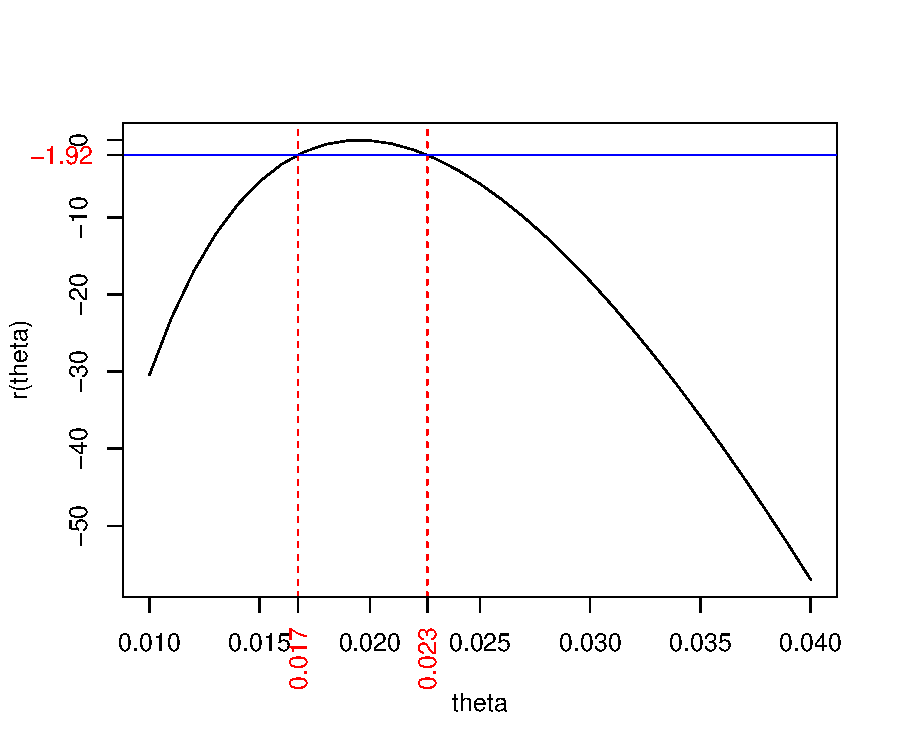
\includegraphics{figures/1bLR.pdf}
            \end{figure}
\end{itemize}
\textcolor{Red}{Wald} based $ \qty{95}{\percent} $ CI: $ \hat{\theta}\pm Z_{0.975}\bigl(I(\hat{\theta})\bigr)^{-1/2} $.
\begin{itemize}
      \item For Binomial distribution $ \hat{\theta}=y/n $ and
            \[ I(\hat{\theta})=\frac{y}{\hat{\theta}^2}+\frac{n-y}{(1-\hat{\theta})^2}=n^2\biggl(\frac{1}{y} +\frac{1}{n-y}\biggr).   \]
      \item So we solve:
            \begin{align*}
                  \hat{\theta}\pm 1.96\bigl(I(\hat{\theta})\bigr)^{-1/2}
                   & =0.0195 \pm 1.96(0.0015) \\
                   & =(0.017, 0.022).
            \end{align*}
      \item The Wald based $ \qty{95}{\percent} $ CI is: $ (0.017, 0.022) $.
\end{itemize}
\subsection*{Hypotheses Test}
Suppose we are interested in testing hypotheses:
\[ \text{$\HN$: $\theta=\theta_0$ vs $\HA$: $\theta\ne \theta_0$.} \]
\begin{itemize}
      \item \textcolor{Red}{Likelihood ratio (LR) test}: $ p\text{-value}=\Prob*{\chi^2_1>-2r(\theta_0)} $.
      \item \textcolor{Red}{Score test}: $ p\text{-value}=\Prob*{\chi^2_1>\bigl(S(\theta)\bigr)^2/I(\theta_0)} $.
      \item \textcolor{Red}{Wald test}:
            \[ p\text{-value}=\Prob*{\chi^2_1>(\hat{\theta}-\theta_0)^2 I(\hat{\theta})}\text{, or }
                  p\text{-value}=\Prob*{\abs{Z}>\abs{\hat{\theta}-\theta_0}\sqrt{I(\hat{\theta})}}. \]
\end{itemize}
\subsection*{Example: Hormone Therapy Data}
Suppose we wish to test if women received EPT would have a risk of breast
cancer same as that of the general population, say about \qty{1.5}{\percent}.
\[ \text{$\HN$: $\theta=0.015$ vs $\HA$: $\theta\ne 0.015$.} \]
\begin{itemize}
      \item \textcolor{Red}{Likelihood Ratio} based test:
            \begin{align*}
                  r(\theta_0=0.015)
                   & =\biggl(y\log{0.015}+(n-y)\log{1-0.15}\biggr)-\biggl(y\log*{\frac{y}{n}}+(n-y)\log*{1-\frac{y}{n} }\biggr) \\
                   & =-5.3637.
            \end{align*}
            Thus, the $ p $-value for the test is given by:
            \[ p=\Prob*{\chi^2_{1}>-2r(0.015)}=\Prob*{\chi^2_{1}>10.7274}=0.001. \]
            Therefore, we \emph{reject} $ \HN $ and conclude that the risk of breast cancer for women received EPT is
            significantly different from \qty{1.5}{\percent}.
\end{itemize}
\subsection*{Notes on Asymptotic Inference}
\begin{itemize}
      \item Asymptotic results: approximation improves as sample size increases.
      \item Results are exact for a Normal linear model if $ \theta $ is the mean parameter and $ \sigma^2 $ is
            known.
      \item \textcolor{Red}{LR approach}:
            \begin{itemize}
                  \item Need to evaluate (log) likelihood at two locations.
                  \item Not always a closed from solution for a CI.
                  \item Usually the best approach.
            \end{itemize}
      \item \textcolor{Red}{Score approach}:
            \begin{itemize}
                  \item Usually the least powerful test.
                  \item Don't actually need to find MLE to use.
            \end{itemize}
      \item \textcolor{Red}{Wald's approach}:
            \begin{itemize}
                  \item Always get a closed form solution for a CI.
                  \item May not behave well for skewed likelihoods (transform?).
            \end{itemize}
      \item All three are asymptotically equivalent!
\end{itemize}
\subsection*{Likelihood Methods for Parameter Vectors}
Suppose $ \Vector{\theta}=(\theta_1,\theta_2,\ldots,\theta_p)^\top\in \Omega $ is a continuous $ p\times 1 $ parameter vector
indexing a probability density (or mass) function $ f(\Vector{y};\Vector{\theta}) $. The likelihood and
log-likelihood functions are defined as before, but
\begin{itemize}
      \item $ \Vector{S}(\Vector{\theta})=\pdv{\ell( \Vector{\theta})}{ \Vector{\theta}} $ is the $ p\times 1 $ \textcolor{Red}{Score vector}, i.e.,
            \[ \Vector{S}(\Vector{\theta})=\begin{bmatrix}
                        \pdv{\ell(\theta)}{\theta_1} \\
                        \vdots                       \\
                        \pdv{\ell(\theta)}{\theta_p}
                  \end{bmatrix}. \]
      \item $ \Matrix{I}(\Vector{\theta})=-\pdv{\ell(\Vector{\theta})}{ \Vector{\theta}^\top,\Vector{\theta}} $ is the $ p\times p $ \textcolor{Red}{Information matrix}, i.e.,
            \[ \Matrix{I}(\Vector{\theta})=\begin{bmatrix}
                        -\pdv[order=2]{\ell(\theta)}{\theta_1} & -\pdv{\ell(\theta)}{\theta_1,\theta_2} & \cdots & \pdv{\ell(\theta)}{\theta_1,\theta_p} \\
                                                               & -\pdv[order=2]{\ell(\theta)}{\theta_2} & \cdots & \pdv{\ell(\theta)}{\theta_1,\theta_p} \\
                                                               &                                        & \ddots & \pdv[order=2]{\ell(\theta)}{\theta_p}
                  \end{bmatrix}. \]

\end{itemize}
\begin{itemize}
      \item The Newton Raphson algorithm applies as before, but with vectors and matrices
            as follows:
            \[ \Vector{\theta}^{(i+1)}=\Vector{\theta}^{(i)}+\Matrix{I}^{-1}(\Vector{\theta}^{(i)})\Vector{S}(\Vector{\theta}^{(i)}). \]
            Again, we apply iteratively until we obtain convergence, but now check to
            see if $ \Matrix{I}(\hat{\Vector{\theta}}) $ is a positive definite matrix.
\end{itemize}
Suppose we want to make inference about a specific parameter in $ \Vector{\theta} $, say we
partition vector $ \Vector{\theta}=(\alpha,\Vector{\beta})^\top $ and \textcolor{Red}{$ \alpha $
      is the parameter of interest}. Analogues to the LR, Score, and Wald results apply, e.g.,
\begin{itemize}
      \item LR statistic: $ -2\bigl[\ell(\alpha,\hat{\Vector{\beta}}_{\alpha})-\ell(\hat{\alpha},\hat{\Vector{\beta}})\bigr]\sim \chi^2_{1} $.
            \begin{itemize}
                  \item $ \hat{\Vector{\beta}}_{\alpha} $ is the MLE of $ \Vector{\beta} $ given $ \alpha $ is fixed.
                  \item $ \hat{\alpha} $ and $ \hat{\Vector{\beta}} $ are the joint MLE of $ \alpha $ and $ \Vector{\beta} $.
            \end{itemize}
      \item Score statistic: $ S_\alpha(\alpha,\hat{\Vector{\beta}}_\alpha)^2 I^{\alpha\alpha}\sim \chi^2_{1} $.
            \begin{itemize}
                  \item $ S_\alpha=\pdv{\ell}{\alpha} $.
                  \item $ I^{\alpha\alpha} $ is the $ (\alpha,\alpha) $ element of $ \Matrix{I}(\alpha,\Vector{\beta})^{-1} $ (inverse of Information matrix).
            \end{itemize}
      \item Wald statistic: $ (\hat{\alpha}-\alpha)^2/I^{\alpha\alpha}\sim \chi^2_{1} $.
\end{itemize}

\chapter{Likelihoods for Generalized Linear Models}
\section*{Topic 2a: Formulation of Generalized Linear Models}
\addcontentsline{toc}{section}{Topic 2a: Formulation of Generalized Linear Models}
\subsection*{The Exponential Family}
\begin{Regular}{Definition (Exponential Family)}
      Consider a random variable $ Y $ with probability density (or mass) function $ f(y;\theta,\phi) $,
      we say that the distribution is a member of the \textcolor{Red}{exponential family} if we can write
      \[ f(y;\theta,\phi)=\exp*{\frac{y\theta-b(\theta)}{a(\phi)}+c(y;\phi)}, \]
      for some functions $ a(\:\cdot\:) $, $ b(\:\cdot\:) $, and $ c(\:\cdot\:) $.
      \begin{itemize}
            \item The parameter $ \theta $ is called the \textcolor{Red}{canonical} parameter, and it is unknown.
            \item The parameter $ \phi $ is called the \textcolor{Red}{scale/dispersion} parameter, is constant, and assumed to be known.
      \end{itemize}
\end{Regular}
Many well known distributions (continuous/discrete) can be shown to be a
member of the exponential family.
\subsection*{Examples}
\begin{itemize}
      \item Poisson Distribution: $ Y \sim \POI{\lambda} $,
            \[ f(y;\lambda)=\frac{\lambda^y \mathrm{e}^{-\lambda}}{y!},\; \lambda>0,\, y=0,1,\ldots.  \]
            Show that Poisson is a member of exponential family and identify the canonical
            parameter and the functions $ a(\:\cdot\:) $, $ b(\:\cdot\:) $, and $ c(\:\cdot\:) $.

            \textbf{Solution.} $ f(y;\lambda)=\exp[\big]{\log{f(y;\lambda)}}=\exp*{\frac{y\log{\lambda}-\lambda}{1} -\log{y!}} $. Therefore,
            \begin{align*}
                  \theta    & =\log{\lambda}\qquad\text{(canonical/natural parameter)}, \\
                  b(\theta) & =\lambda=\mathrm{e}^{\theta},                             \\
                  \phi      & =1,                                                       \\
                  a(\phi)   & =1,                                                       \\
                  c(y;\phi) & =-\log{y!}.
            \end{align*}
      \item Normal Distribution: $ Y \sim \N{\mu,\sigma^2} $ and $ \sigma^2 $ known,
            \[ f(y;\theta,\phi)=\frac{1}{\sqrt{2\pi\sigma^2}}\exp*{-\frac{(y-\mu)^2}{2\sigma^2}}. \]
            Show that this Normal distribution is a member of the exponential family.

            \textbf{Solution.}
            \begin{align*}
                  f(y;\mu,\sigma^2)
                   & =\exp*{-\frac{y^2-2\mu y+\mu^2}{\sigma^2}-\frac{1}{2} \log{2\pi\sigma^2}}                   \\
                   & =\exp*{\frac{y\mu-\mu^2/2}{\sigma^2}-\frac{y^2}{2\sigma^2}-\frac{1}{2} \log{2\pi\sigma^2}}.
            \end{align*}
            Therefore,
            \begin{align*}
                  \theta    & =\mu,                                                   \\
                  \phi      & =\sigma^2,                                              \\
                  a(\phi)   & =\phi=\sigma^2,                                         \\
                  b(\theta) & =\frac{\mu^2}{2}=\frac{\theta^2}{2},                    \\
                  c(y;\phi) & =-\frac{y^2}{2\sigma^2}-\frac{1}{2} \log{2\pi\sigma^2}.
            \end{align*}
\end{itemize}
\subsection*{Properties of Exponential Family}
Consider a single observation $y$ from the exponential family.
\begin{align*}
      L(\theta,\phi;y)    & =f(y;\theta,\phi)=\exp*{\frac{y\theta-b(\theta)}{a(\phi)}+c(y;\phi)}.      \\
      \ell(\theta,\phi;y) & =\log[\big]{f(y;\theta,\phi)}=\frac{y\theta-b(\theta)}{a(\phi)}+c(y;\phi). \\
      S(\theta)           & =\pdv{\ell}{\theta}=\frac{y-b^\prime(\theta)}{a(\phi)}.                    \\
      I(\theta)           & =-\pdv[order=2]{\ell}{\theta}=\frac{b^{\prime\prime}(\theta)}{a(\phi)}.    \\
      \mathcal{I}(\theta) & =\E*{-\pdv[order=2]{\ell}{\theta}}=I(\theta).
\end{align*}
\subsection*{Some General Results for Score and Information}
\begin{Result}{Result \# 1}
      The expectation of the score function is zero.
      \[ \E[\big]{S(\theta)}=0. \]
      \tcblower{}
      \textbf{Proof}:
      \begin{align*}
            \int f(y;\theta,\phi)\odif{y}                                                         & =1                               \\
            \pdv*{\int f(y;\theta,\phi)\odif{y}}{\theta}                                          & =0                               \\
            \int\pdv*{f(y;\theta,\phi)}{\theta} \odif{y}                                          & =0                               \\
            \int\biggl(\pdv*{\log[\big]{f(y;\theta,\phi)}}{\theta}\biggr)f(y;\theta,\phi)\odif{y} & =0 &  & \label{2a:eq1}\tag*{(1)} \\
            \int S(\theta)f(y;\theta,\phi)\odif{y}                                                & =0                               \\
            \E[\big]{S(\theta)}                                                                   & =0
      \end{align*}
\end{Result}
\begin{Result}{Result \# 2}
      The expectation of the score function squared is the expected information.
      \[  \E[\big]{S(\theta;y)^2}=\E[\big]{I(\theta;y)} \]
      \tcblower{}
      \textbf{Proof}: Differentiate~\ref{2a:eq1} again,
      \begin{align*}
            \pdv*{\int\biggl(\pdv*{\log[\big]{f(y;\theta,\phi)}}{\theta}\biggr)f(y;\theta,\phi)\odif{y}}{\theta}                                                                                                 & =0 \\
            \int \biggl(\pdv*[order=2]{\log[\big]{f(y;\theta,\phi)}}{\theta}\biggr)f(y;\theta,\phi)\odif{y}+\int\biggl(\pdv*{\log[\big]{f(y;\theta,\phi)}}{\theta}\biggr)\pdv*{f(y;\theta,\phi)}{\theta}\odif{y} & =0 \\
            \int \pdv*[order=2]{\log[\big]{f(y;\theta,\phi)}}{\theta}f(y;\theta,\phi)\odif{y}+\int\biggl(\pdv*{f(y;\theta,\phi)}{\theta}\biggr)^2 f(y;\theta,\phi)\odif{y}                                       & =0 \\
            \int -I(\theta)f(y;\theta,\phi)\odif{y}+\int S(\theta)^2 f(y;\theta,\phi)\odif{y}                                                                                                                    & =0 \\
            \E[\big]{-I(\theta;y)}+\E[\big]{S(\theta;y)^2}                                                                                                                                                       & =0
      \end{align*}
\end{Result}
Now for the exponential family, we apply above results and obtain:
\begin{align*}
      \E[\big]{S(\theta)}                                          & =0,                                             \\
      \E*{\frac{Y-b^{\prime}(\theta)}{a(\phi)}}                    & =0,                                             \\
      \E{Y}                                                        & =b^\prime(\theta),                              \\\\
      \E[\big]{S(\theta)^2}                                        & =\E[\big]{I(\theta)},                           \\
      \E*{\biggl(\frac{Y-b^\prime(\theta)}{a(\phi)} \biggr)^{\!2}} & =\E*{\frac{b^{\prime\prime}(\theta)}{a(\phi)}}, \\
      \frac{1}{a(\phi)^2}\E*{\bigl(Y-\E{Y}\bigr)^2}                & =\frac{b^{\prime\prime}(\theta)}{a(\phi)},      \\
      \Var{Y}                                                      & =b^{\prime\prime}(\theta)a(\phi).
\end{align*}
\begin{Regular}{Mean and Variance for the Exponential Family}
      \begin{itemize}
            \item Mean: $ \E{Y}=b^\prime(\theta)=\mu $.
            \item Variance: $ \Var{Y}=b^{\prime\prime}(\theta)a(\phi) $.
      \end{itemize}
\end{Regular}
Note that:
\begin{itemize}
      \item $ b^\prime(\theta)=\mu $ tells the relationship between \emph{canonical} parameter $ \theta $ and $ \mu $.
      \item $ b^{\prime\prime}(\theta) $ is a function of $ \theta $ and hence can be also expressed as a function of $ \mu $.
      \item Thus, we write $ b^{\prime\prime}(\theta)=\V{\mu} $ and call \textcolor{Red}{$ \V{\mu} $} the \textcolor{Red}{variance function}.
      \item Subsequently, we have:
            \[ \Var{Y}=b^{\prime\prime}(\theta)a(\phi)=\V{\mu}a(\phi), \]
            which is the \textcolor{Red}{mean-variance relationship} for the exponential family.
\end{itemize}
\subsection*{Link Functions}
\begin{Regular}{Definition (Link Function)}
      The \textcolor{Red}{link function} relates the linear predictor $ \eta=\Vector{x}^\top\Vector{\beta} $ to the expected value $ \mu $ of the random variable $ Y $, i.e.,
      \[ g(\mu)=\eta=\Vector{x}^\top\Vector{\beta}, \]
      where $ g(\:\cdot\:) $ is the link function.
\end{Regular}
\begin{Regular}{Definition (Canonical Link Function)}
      When $Y$ is a member of the exponential family we define the \textcolor{Red}{canonical link function} to be:
      \[ g(\mu)=\theta=\eta=\Vector{x}^\top\Vector{\beta} \]
      (i.e., the choice of $ g(\:\cdot\:) $ that sets canonical parameter = linear predictor).
\end{Regular}
\subsection*{Example}
Recall that $ \POI{\lambda} $ is a member of exponential family,
\[ f(y;\lambda)=\frac{\lambda^y \mathrm{e}^{-\lambda}}{y!}=\exp*{\frac{y\log{\lambda}-\lambda}{1}-\log{y!}}  \]
where $ \theta=\log{\lambda} $, $ \phi=1 $, $ b(\theta)=\lambda=\mathrm{e}^{\theta} $, and $ a(\phi)=1 $. Now to find the mean, variance function, and canonical link function:
\begin{itemize}
      \item \textcolor{Blue}{Mean}: $ \E{Y}=b^\prime(\theta)=\mathrm{e}^{\theta}=\mu\implies \theta=\log{\mu} $.
      \item \textcolor{Blue}{Variance Function}: $ \V{\mu}=b^{\prime\prime}(\theta)=\mathrm{e}^{\theta}\implies \V{\mu}=\mu $.
      \item \textcolor{Blue}{Variance}: $ \Var{Y}=\V{\mu}a(\phi)=\mu $ (mean-variance relationship).
      \item \textcolor{Blue}{Canonical link}: set $ \theta=\eta $ using $ \theta=\log{\mu}=\eta=\Vector{x}^\top \Vector{\beta} $, i.e., $ g(\mu)=\log{\mu} $ where $ \log{\:\cdot\:} $
            is the canonical link.
\end{itemize}
Moving forward, we consider a log-linear model: $ \log{\mu_i}=\Vector{x}_i^\top \Vector{\beta} $.

\subsection*{Remarks on Link Function}
\begin{itemize}
      \item We can choose any function $ g(\:\cdot\:) $ as the link function in theory.
      \item The canonical link is a special link function, we often choose to use
            canonical link for its good statistical properties.
      \item Context and goodness of fit should motivate the choice of link function in
            practice.
\end{itemize}
\subsection*{Generalized Linear Models}
\begin{Regular}{Definition (Generalized Linear Model (GLM))}
      A \textcolor{Red}{Generalized Linear Model (GLM)} is composed of three components:
      \begin{itemize}
            \item \textcolor{Red}{Random Component}: The responses $ Y_1,\ldots,Y_n $ are
                  independent random variables and each $ Y_i $ is assumed to come from a parametric distribution that is a member of the
                  exponential family.
            \item \textcolor{Red}{Systematic Component} (or linear predictor):
                  \[ \eta_i=\Vector{x}_i^\top\Vector{\beta}, \]
                  a linear combination of explanatory variables $ \Vector{x}_i $ and regression parameters $ \Vector{\beta} $.
            \item \textcolor{Red}{Link function}:
                  \[ g(\mu_i)=\eta_i=\Vector{x}_i^\top\Vector{\beta}, \]
                  a function that relates the mean of response to the linear predictor.
      \end{itemize}
\end{Regular}
\subsection*{Topic Summary}
2a Formulation of Generalized Linear Models:
\begin{itemize}
      \item Definition of the \textcolor{Blue}{Exponential Family}.
            \begin{itemize}
                  \item Exponential form of the probability density (or mass) function.
                  \item Derivation of Score and Information.
                  \item Properties of exponential family, mean-variance relationship.
                  \item Definition of canonical link.
            \end{itemize}
      \item Definition of a \textcolor{Blue}{Generalized Linear Model}.
\end{itemize}
Next Topic: 2b Estimation for Generalized Linear Models.
% Week 3

\makeheading{Week 3}{\daterange{2021-09-20}{2021-09-24}}
\section*{Topic 2b: Maximum Likelihood Estimation for Generalized Linear Models}
\addcontentsline{toc}{section}{Topic 2a: Maximum Likelihood Estimation for Generalized Linear Models}
\subsection*{Generalized Linear Models}
Suppose for each subject $ i=1,\ldots,n $ in a random sample:
\begin{itemize}
    \item $ Y_i $ is the response variable.
    \item $ x_{i1},\ldots,x_{ip} $ are explanatory variables associated with $ Y_i $.
\end{itemize}
We consider a \textcolor{Red}{Generalized Linear Model} (GLM) for the data, by definition the GLM
is composed following three components:
\begin{Regular}{}
    \begin{enumerate}[label=\color{Blue}\protect\circled{\arabic*}]
        \item \textcolor{Red}{Random Component}:
              \[ Y_i \sim \text{exponential family,}\qquad Y_1,\ldots,Y_n\text{ are independent.} \]
        \item \textcolor{Red}{Systematic Component} (or linear predictor):
              \[ \eta_i=\Vector{x}_i^\top \Vector{\beta}=\beta_0+\beta_1x_{i1}+\cdots+\beta_p x_{ip}. \]
              \begin{itemize}
                  \item $ \Vector{x}_i=(1,x_{i1},\ldots,x_{ip})^\top $ is a covariate vector.
                  \item $ \Vector{\beta}=(\beta_0,\beta_1,\ldots,\beta_p)^\top $ is a vector of regression coefficients.
              \end{itemize}
        \item \textcolor{Red}{Link function}: a function $ g(\:\cdot\:) $ links $ \E{Y_i}=\mu_i $ to a linear prediction $ \eta_i $:
              \[ g(\mu_i)=\eta_i=\Vector{x}_i^\top\Vector{\beta}. \]
    \end{enumerate}
\end{Regular}
\subsection*{Example: A Poisson Regression Model}
Suppose $ Y_i \ind\POI{\lambda_i} $ with mean $ \E{Y_i}=\lambda_i $, $ i=1,\ldots,n $:
\[ f(y_i)=\frac{\mathrm{e}^{-\lambda_i}\lambda_i^{y_i}}{y_i!}=\exp[\big]{y_i\log{\lambda_i}-\lambda_i-\log{y_i!}}.  \]
Poisson distribution is a member of exponential family with:
\begin{itemize}
    \item Canonical parameter: $ \theta_i=\log{\lambda_i} $.
    \item Canonical link: $ \theta_i=\eta_i\textcolor{Red}{\implies}\log{\lambda_i}=\Vector{x}_i^\top \Vector{\beta} $ (log link).
\end{itemize}
A Poisson regression model with the canonical link takes the form:
\[ \log{\lambda_i}=\Vector{x}_i^\top \Vector{\beta}=\beta_0+\beta_1x_{i1}+\cdots+\beta_p x_{ip}\qquad \text{\textcolor{Red}{(log-linear model)}}. \]
\subsection*{Example: A Normal Regression Model}
Assume $ Y_i \ind \N{\mu_i,\sigma^2} $ and $ \sigma^2 $ is known, $ i=1,\ldots,n $:
\begin{align*}
    f(y_i)
     & =(2\pi\sigma^2)^{-1/2}\exp*{-\frac{(y_i-\mu_i)^2}{2\sigma^2}}                                                   \\
     & =\exp*{\frac{y_i\mu_i-\mu_i^2/2}{\sigma^2}-\frac{1}{2}\biggl(\frac{y_i^2}{\sigma^2}+\log{2\pi\sigma^2}\biggr)}.
\end{align*}
A Normal distribution ($ \sigma^2 $ known) is a member of exponential family with:
\begin{itemize}
    \item Canonical parameter: $ \theta_i=\mu_i $.
    \item Canonical link: $ \theta_i=\eta_i \textcolor{Red}{\implies}\mu_i=\Vector{x}_i^\top \Vector{\beta} $ (identity link).
\end{itemize}
A Normal regression model with the canonical link takes the form:
\[ \mu_i=\Vector{x}_i^\top \Vector{\beta}=\beta_0+\beta_1x_{i1}+\cdots+\beta_p x_{ip}\qquad \text{\textcolor{Red}{(linear model)}}. \]
Linear regression model (STAT 331) is a Normal GLM using the canonical link!
\subsection*{Likelihood for Generalized Linear Models}
We wish to use likelihood methods for the estimation of the regression parameter $ \Vector{\beta} $ from the GLM: $ g(\mu_i)=\Vector{x}_i^\top \Vector{\beta} $.
Consider the log-likelihood for a \emph{single} observation from the exponential family:
\[ \ell(\theta,\phi;y)=\frac{y\theta-b(\theta)}{a(\phi)}+c(y;\phi). \]
\begin{itemize}
    \item $ \ell $ is a function of $ \textcolor{Red}{\theta} $ (assume that $ \phi $ is known).
    \item $ \theta $ is related to $ \mu $ through the result:
          \[ \textcolor{Red}{\mu=b^{\prime}(\theta)}. \]
    \item $ \eta $ can be expressed in terms of $ \mu $ through the link function:
          \[ \textcolor{Red}{g(\mu)=\eta}. \]
    \item $ \Vector{\beta} $ can be expressed in terms of $ \eta $ through the linear predictor:
          \[ \textcolor{Red}{\eta=\Vector{x}^\top \Vector{\beta}}. \]
\end{itemize}
\subsection*{Score Vector}
To find the maximum likelihood estimator for $ \Vector{\beta} $, we must solve $ \Vector{S}(\Vector{\beta})=\pdv{\ell}{\Vector{\beta}}=\Vector{0} $.
Consider taking derivative with respect to $ \beta_j $ using the chain rule:
\[ \pdv{\ell}{\beta_j}=\pdv{\ell}{\theta}\pdv{\theta}{\mu}\pdv{\mu}{\eta}\pdv{\eta}{\beta_j}, \]
where
\begin{align*}
    \pdv{\ell}{\theta}  & =\frac{y-b^{\prime}(\theta)}{a(\phi)},                                                                                                          \\
    \pdv{\theta}{\mu}   & =\pdv{\mu}{\theta}^{\!-1}=\frac{1}{b^{\prime\prime}(\theta)} &  & \text{since $ \mu=b^\prime(\theta) $},                                        \\
    \pdv{\mu}{\eta}     & =\pdv{\mu}{\eta},                                                                                                                               \\
    \pdv{\eta}{\beta_j} & =x_j                                                         &  & \text{since $ \eta=\beta_0+\beta_1x_1+\cdots+\beta_jx_j+\cdots+\beta_px_p $}.
\end{align*}
Hence, we have:
\begin{align*}
    \pdv{\ell}{\beta_j}
     & =\frac{y-b^{\prime}(\theta)}{a(\phi)}\frac{1}{b^{\prime\prime}(\theta)}\pdv{\mu}{\eta}x_j                                                                                           \\
     & =\frac{y-\mu}{\Var{Y}}\pdv{\mu}{\eta}x_j                                                  &  & \text{since $ \mu=b^{\prime}(\theta) $, $ \Var{Y}=a(\phi)b^{\prime\prime}(\theta) $} \\
     & =\frac{y-\mu}{\Var{Y}}\pdv{\mu}{\eta}^{\!2}\pdv{\eta}{\mu}x_j                             &  & \text{since $ \pdv{\mu}{\eta}\pdv{\eta}{\mu}=1 $}                                    \\
     & =(y-\mu)\Biggl(\Var{Y}\pdv{\mu}{\eta}^{\!2}\Biggr)^{\!-1}\pdv{\eta}{\mu}x_j                                                                                                         \\
     & =(y-\mu)W\pdv{\eta}{\mu}x_j,
\end{align*}
where $ W^{-1}=\Var{Y}\pdv{\eta}{\mu}^2 $. Note that generally $ \pdv{\eta}{\mu} $ is easier to calculate
than $ \pdv{\mu}{\eta} $ since we define the link as $ \eta=g(\mu) $.

For a random sample $ Y_1,\ldots,Y_n $ from exponential family and each $ Y_i $ has a probability density function
\[ f(y_i;\theta,\phi)=\exp*{\frac{y_i\theta_i-b(\theta_i)}{a(\phi)}+c(y_i,\phi)}. \]
We write likelihood and log-likelihood functions as:
\begin{align*}
    L    & =\prod_{i=1}^n f(y_i;\theta_i,\phi)=\prod_{i=1}^n\exp*{\frac{y_i\theta_i-b(\theta_i)}{a(\phi)}+c(y_i,\phi)}, \\
    \ell & =\sum_{i=1}^{n} \ell_i=\sum_{i=1}^{n}\frac{y_i\theta_i-b(\theta_i)}{a(\phi)}+c(y_i,\phi).
\end{align*}
The \textcolor{Red}{element of the score vector} is:
\[ \bigl[\Vector{S}(\Vector{\beta})\bigr]_j=\pdv{\ell}{\beta_j}=\sum_{i=1}^{n} \pdv{\ell_i}{\beta_j}=\sum_{i=1}^{n} (y_i-\mu_i)W_i\pdv{\eta_i}{\mu_i}x_{ij} \]
where $  W_i^{-1}=\Var{Y_i}(\pdv{\eta_i}{\mu_i})^2 $, $ g(\mu_i)=\eta_i=\Vector{x}_i^\top \Vector{\beta} $. In vector and matrix form we can write:
\[ \Vector{S}(\Vector{\beta})=\Matrix{X}\MatrixCal{W}\MatrixCal{A}(\Vector{y}-\Vector{\mu}), \]
where
\begin{itemize}
    \item $ \Vector{y}=(y_1,\ldots,y_n)^\top $ and $ \Vector{\mu}=(\mu_1,\ldots,\mu_n)^\top $ are $ n\times 1 $ vectors,
    \item $ \Matrix{X}=(\Vector{x}_1,\ldots,\Vector{x}_n) $ is a $ (p+1)\times n $ matrix,
    \item $ \MatrixCal{W}=\diag{W_1,\ldots,W_n}=\begin{bmatrix}
                  W_1    & 0      & \cdots & 0      \\
                  \vdots & \ddots & \ddots & \vdots \\
                  0      & \cdots & 0      & W_n
              \end{bmatrix} $, and
    \item $ \MatrixCal{A}=\diag*{\pdv{\eta_1}{\mu_1},\ldots,\pdv{\eta_n}{\mu_n}} $.
\end{itemize}
\subsection*{Example: Poisson Regression Model (Problem 1.4)}
For a random sample from Poisson distribution, $ Y_i \sim \POI{\lambda_i} $, $ i=1,\ldots,n $,
\[ \ell_i=\log[\big]{f(y_i;\lambda_i)}=\bigl(y_i\log{\lambda_i}-\lambda_i-\log{y_i!}\bigr). \]
Poisson regression with a log-link:
\[ \log{\lambda_i}=\eta_i=\Vector{x}_i^\top \Vector{\beta}. \]
To write down the score vector for the regression coefficients $ \Vector{\beta} $, we may
calculate the derivative using standard methods, i.e.,
\begin{align*}
    \bigl[\Vector{S}(\Vector{\beta})\bigr]_j
     & =\sum_i \pdv{\ell_i}{\beta_j}                                                                                  \\
     & =\sum_i \pdv*{\bigl(y_i \textcolor{Red}{\log{\lambda_i}}-\textcolor{Red}{\lambda_i}-\log{y_i!}\bigr)}{\beta_j} \\
     & =\sum_i\bigl(y_i x_{ij}-\mathrm{e}^{\Vector{x}_i^\top \Vector{\beta}}x_{ij}\bigr).
\end{align*}
Or we can use the general results derived for the GLMs on the previous slides.
\subsection*{Solving $ \Vector{S}(\Vector{\beta})=\Vector{0} $ for MLE}
\begin{enumerate}[label=\color{Blue}\protect\circled{\arabic*}]
    \item Newton Raphson update equation is:
          \[ \hat{\Vector{\beta}}^{(r+1)}=\hat{\Vector{\beta}}^{(r)}+\Matrix{I}^{-1}(\hat{\Vector{\beta}}^{(r)})\Vector{S}(\hat{\Vector{\beta}}^{(r)}), \]
          where $ \Matrix{I} $ is the observed information matrix.
          \begin{itemize}
              \item This requires us to find and repeatedly evaluate the information $ \Matrix{I} $ (possibly computationally intensive).
              \item Fisher suggested using the expected information matrix $ \MatrixCal{I} $ rather than the observed information matrix.
          \end{itemize}
    \item Fisher Scoring update equation is:
          \[ \hat{\Vector{\beta}}^{(r+1)}=\hat{\Vector{\beta}}^{(r)}+\MatrixCal{I}^{-1}(\hat{\Vector{\beta}}^{(r)})\Vector{S}(\hat{\Vector{\beta}}^{(r)}). \]
\end{enumerate}
\subsection*{Information Matrix}
Consider the $(j, k)$ element of the Information matrix:
\begin{align*}
    \Matrix{I}_{jk} & =-\pdv{\ell}{\beta_j,\beta_k}                                                                                                                                                                                     \\
                    & =-\pdv*{\pdv{\ell}{\beta_j}}{\beta_k}                                                                                                                                                                             \\
                    & =\sum_i -\pdv*{\biggl[(y_i-\mu_i)W_i\biggl(\pdv{\eta_i}{\mu_i}\biggr)x_{ij}\biggr]}{\beta_k}                                                                                                                      \\
                    & =\sum_i -(y_i-\mu_i)\Biggl\{\pdv*{\biggl[W_i\biggl(\pdv{\eta_i}{\mu_i}\biggr)x_{ij}\biggr]}{\beta_k}\Biggr\}-W_i\biggl(\pdv{\eta_i}{\mu_i}\biggr)x_{ij}\biggl(\textcolor{Red}{\pdv*{(y_i-\mu_i)}{\beta_k}}\biggr) \\
                    & =\sum_i -(y_i-\mu_i)\Biggl\{\pdv*{\biggl[W_i\biggl(\pdv{\eta_i}{\mu_i}\biggr)x_{ij}\biggr]}{\beta_k}\Biggr\}+W_i\biggl(\pdv{\eta_i}{\mu_i}\biggr)x_{ij}\textcolor{Red}{\pdv{\mu_i}{\eta_i}\pdv{\eta_i}{\beta_k}}  \\
                    & =\sum_i -(y_i-\mu_i)\pdv*{\biggl[W_i\biggl(\pdv{\eta_i}{\mu_i}\biggr)x_{ij}\biggr]}{\beta_k}+x_{ij}W_i x_{ik}.
\end{align*}
\subsection*{Fisher Information}
To get an element of the Expected/Fisher Information matrix:
\begin{align*}
    \MatrixCal{I}_{jk}
     & =\sum_i\E*{-\pdv{\ell}{\beta_j,\beta_k}}                                                                                                \\
     & =\sum_i\E*{-(Y_i-\mu_i)\pdv*{\biggl[W_i\biggl(\pdv{\eta_i}{\mu_i}\biggr)x_{ij}\biggr]}{\beta_k}+x_{ij}W_i x_{ik}}                       \\
     & =\sum_i-\textcolor{Red}{\E[\big]{(Y_i-\mu_i)}}\pdv*{\biggl[W_i\biggl(\pdv{\eta_i}{\mu_i}\biggr)x_{ij}\biggr]}{\beta_k}+x_{ij}W_i x_{ik} \\
     & =\sum_i x_{ij}W_i x_{ik}.
\end{align*}
Therefore, we can write the $(j, k)$ element of the Fisher information as:
\[ \MatrixCal{I}_{jk}=\sum_{i=1}^{n} x_{ij}W_i x_{ik}=[\Matrix{X}\Matrix{\MatrixCal{W}}\Matrix{X}^\top]_{jk} \]
where again, $ \MatrixCal{W}=\diag{W_1,\ldots,W_n} $ and $ W_i^{-1}=\Var{Y_i}\pdv{\eta_i}{\mu_i}^2 $.
\subsection*{When is Fisher Scoring Equivalent to Newton Raphson?}
Recall information matrix:
\[  \Matrix{I}_{jk}=\sum_i -(y_i-\mu_i)\pdv*{\biggl[\textcolor{Red}{W_i\biggl(\pdv{\eta_i}{\mu_i}\biggr)x_{ij}}\biggr]}{\beta_k}+x_{ij}W_i x_{ik}. \]
Now examine:
\begin{align*}
    W_i\biggl(\pdv{\eta_i}{\mu_i}\biggr)x_{ij}
     & =\Biggl(\Var{Y_i}\biggl(\pdv{\eta_i}{\mu_i}\biggr)^{\!2}\Biggr)^{\!-1}\biggl(\pdv{\eta_i}{\mu_i}\biggr)x_{ij}                                                                                                        \\
     & =\Biggl(a(\phi)b^{\prime\prime}(\theta_i)\pdv{\eta_i}{\mu_i}\Biggr)^{\!-1}x_{ij}                              &  & \text{since $\Var{Y_i}=a_i(\phi)b^{\prime\prime}(\theta_i)$}                                      \\
     & =\Biggl(a(\phi)\pdv{\mu_i}{\theta_i}\pdv{\eta_i}{\mu_i} \Biggr)^{\!-1}x_{ij}                                  &  & \text{since $ b^{\prime}(\theta_i)=\mu_i $, $ b^{\prime\prime}(\theta_i)=\pdv{\mu_i}{\theta_i} $} \\
     & =\bigl(a(\phi)\bigr)^{-1}x_{ij}                                                                               &  & \text{\textcolor{Red}{under the canonical link $\theta_i=\eta_i$.}}
\end{align*}
So under the \textcolor{Red}{canonical link},
\[ \pdv*{\biggl[W_i\biggl(\pdv{\eta_i}{\mu_i}\biggr)x_{ij}\biggr]}{\beta_k}=\pdv*{\Bigl[\textcolor{Red}{\bigl(a(\phi)\bigr)^{-1}x_{ij}}\Bigr]}{\beta_k}=0, \]
therefore information matrix is same as the Fisher information:
\[ \Matrix{I}_{jk}=\sum_{i}x_{ij}W_i x_{ij}=\MatrixCal{I}_{jk}  \]
and Fisher Scoring is equivalent to Newton Raphson.
\subsection*{Iteratively Reweighted Least Squares}
The Fisher Scoring is also called \textcolor{Red}{iteratively reweighted least squares} (IRWLS).
The reason is that the update equation can be rewritten as:
\[ \hat{\Vector{\beta}}^{(r+1)}=\Bigl(\Matrix{X}\MatrixCal{W}\bigl(\hat{\Vector{\beta}}^{(r)}\bigr)\Matrix{X}^\top\Bigr)^{\!-1}\Matrix{X}\MatrixCal{W}\bigl(\hat{\Vector{\beta}}^{(r)}\bigr)\RandomVector{Z}\bigl(\hat{\Vector{\beta}}^{(r)}\bigr) \]
where $ \RandomVector{Z} $ is a transformation of the response vector $ \RandomVector{Y} $ such that:
\[ \RandomVector{Z}=\Vector{\eta}+(\RandomVector{Y}-\Vector{\mu})\ast\pdv{\Vector{\eta}}{\Vector{\mu}} \]
\begin{itemize}
    \item See manipulation in Section 1.2.3 of course notes.
    \item Same form as the weighted LS estimate of $ \Vector{\beta} $ with dependent variable $ \RandomVector{Z} $
          and weight matrix $ \MatrixCal{W} $.
    \item $ \RandomVector{Z} $ and $ \MatrixCal{W} $ are updated at each iteration.
\end{itemize}
\subsection*{Topic Summary}
2b Maximum Likelihood Estimation of Generalized Linear Models:
\begin{itemize}
    \item When $ Y_i $ come from a distribution in the \textcolor{Red}{exponential family}, we can use
          the theory of \textcolor{Red}{Generalized Linear Models} to fit the regression equations of
          the form:
          \[ g(\mu_i)=\Vector{x}_i^\top \Vector{\beta}. \]
    \item The \textcolor{Red}{link function} $ g(\:\cdot\:) $ may be the canonical link, but its choice should
          come from model interpretation and fit.
    \item Can use Fisher Scoring (also known as IRWLS) to estimate the regression parameters $ \Vector{\beta} $ from any GLM based on general forms for $ \Matrix{I}(\Vector{\beta}) $
          and $ \Vector{S}(\Vector{\beta}) $.
    \item \textcolor{Blue}{\textsc{Practice}}: Chapter 1 review problems.
\end{itemize}

\chapter{Basic methods for the Analysis of Binary Data}
\section*{Topic 3a: Binary Data and Odds Ratios}
\addcontentsline{toc}{section}{Topic 3a: Binary Data and Odds Ratios}
\subsection*{Binary Data Set-up}
\begin{itemize}
      \item Consider the simplest case with two \emph{binary} variables:
            \begin{itemize}
                  \item COVID-19: infected or not infected (response).
                  \item Vaccination: yes or no (explanatory variable).
            \end{itemize}
      \item Use a $ 2\times 2 $ table to summarize the data:
            \begin{table}[!htbp]
                  \centering
                  \begin{NiceTabular}{c|cc|c}
                        & \multicolumn{2}{c}{\emph{COVID-19}}                                                 \\
                        Vaccination & infected                            & not infected                                        \\
                        \midrule
                        yes & $ y_1 $                            & $ m_1-y_1 $                 & $ m_1 $         \\
                        no   & $ y_2 $                            & $ m_2-y_2 $                 & $ m_2 $         \\
                        \midrule
                        Total& $ y_{\bullet} $                    & $ m_{\bullet}-y_{\bullet} $ & $ m_{\bullet} $
                  \end{NiceTabular}
            \end{table}
      \item Treat $ m_1 $ and $ m_2 $ as fixed, assume $ Y_1 $ and $ Y_2 $ are independent binomial r.v.'s
            \[ \textcolor{Red}{Y_k \sim \BIN{m_k,\pi_k},\qquad k=1,2,} \]
            where $ \pi_k=\Prob{\text{infection}\given \text{group $ k $}} $.
      \item How do we measure the associate between COVID-19 infection and vaccination?
\end{itemize}

\subsection*{Measures of Association}
\begin{Regular}{Definition (Odds Ratio)}
      The \textcolor{Red}{Odds Ratio} (OR) is the ratio of the odds of an event occurring in one
      group to the odds of the event in another group (e.g., not vaccinated):
      \[ \text{Odds Ratio}=\frac{\pi_1/(1-\pi_1)}{\pi_2/(1-\pi_2)}. \]
\end{Regular}
Interpretation of OR:
\[ \begin{array}{ccccc}
            \pi_1=\pi_2 & \implies & \OR=1   & \implies & \text{equal risk (no association)} \\
            \pi_1>\pi_2 & \implies & \OR>1   & \implies & \text{higher risk in group 1}      \\
            \pi_1<\pi_2 & \implies & 0<\OR<1 & \implies & \text{higher risk in group 2}
      \end{array} \]
\begin{Regular}{Relative Risk (RR)}
      The \textcolor{Red}{Relative Risk} (RR) is the ratio of the probability of an event occurring in one group versus another group:
      \[ \text{Relative Risk}=\frac{\pi_1}{\pi_2} \]
\end{Regular}
In the case of a \textcolor{Red}{rare disease} (i.e., when $ \pi_1 $ and $ \pi_2 $ are very small),
\[ \OR=\frac{\pi_1/(1-\pi_1)}{\pi_2/(1-\pi_2)}=\frac{\pi_1}{\pi_2}\underbrace{\biggl(\frac{1-\pi_2}{1-\pi_1}\biggr)}_{\approx 1}\approx \frac{\pi_1}{\pi_2} =\RR,  \]
then
\[ \OR\approx\RR. \]
\subsection*{Maximum Likelihood Estimation of Odds Ratio}
\begin{itemize}
      \item Goal: Estimate odds ratio $ \psi=\frac{\pi_1/(1-\pi_1)}{\pi_2/(1-\pi_2)} $ using likelihood method. Based
            on ``grouped'' binomial data, $ \textcolor{Red}{Y_k \sim \BIN{m_k,\pi_k},\; k=1,2} $,
            \begin{align*}
                  L(\pi_1,\pi_2)
                   & =\binom{m_1}{y_1}\pi_1^{y_1}(1-\pi_1)^{m_1-y_1}\binom{m_2}{y_2}\pi_2^{y_2}(1-\pi_2)^{m_2-y_2}                                                        \\
                   & \propto\biggl(\frac{\pi_1/(1-\pi_1)}{\pi_2/(1-\pi_2)} \biggr)^{\!y_1}\biggl(\frac{\pi_2}{1-\pi_2}\biggr)^{\! y_2+y_1}(1-\pi_1)^{m_1}(1-\pi_2)^{m_2}.
            \end{align*}
      \item Note that $ \pi_1,\pi_2\in[0,1] $ and odds ratio $ \psi\in(0,\infty) $ are restricted, we consider re-parameterize:
            \[ \theta_1=\log*{\frac{\pi_1/(1-\pi_1)}{\pi_2/(1-\pi_2)}}=\log{\psi},\qquad \theta_2=\log*{\frac{\pi_2}{1-\pi_2}}, \]
            and now $ \theta_1,\theta_2\in(-\infty,\infty) $.
      \item Our re-parameterization implies:
            \[ \pi_1=\frac{\mathrm{e}^{\theta_1+\theta_2}}{1+\mathrm{e}^{\theta_1+\theta_2}},\qquad \pi_2=\frac{\mathrm{e}^{\theta_2}}{1+\mathrm{e}^{\theta_2}}. \]
            Now the likelihood becomes:
            \begin{align*}
                  L(\theta_1,\theta_2)    & =(\mathrm{e}^{\theta_1})^{y_1}(\mathrm{e}^{\theta_2})^{y_1+y_2}(1+\mathrm{e}^{\theta_1+\theta_2})^{m_1}(1+\mathrm{e}^{\theta_2})^{-m_2}, \\
                  \ell(\theta_1,\theta_2) & =y_1\theta_1+(y_1+y_2)\theta_2-m_1\log{1+\mathrm{e}^{\theta_1+\theta_2}}-m_2\log{1+\mathrm{e}^{\theta_2}}.
            \end{align*}
      \item The score vector is:
            \[ S(\theta_1,\theta_2)=\begin{pmatrix}
                        \pdv{\ell}{\theta_1} \\
                        \pdv{\ell}{\theta_2}
                  \end{pmatrix}=\begin{pmatrix}
                        y_1-m_1\biggl(\frac{\mathrm{e}^{\theta_1+\theta_2}}{1+\mathrm{e}^{\theta_1+\theta_2}} \biggr) \\
                        y_1+y_2-m_1\biggl(\frac{\mathrm{e}^{\theta_1+\theta_2}}{1+\mathrm{e}^{\theta_1+\theta_2}} \biggr)-m_2\biggl(\frac{\mathrm{e}^{\theta_2}}{1+\mathrm{e}^{\theta_2}} \biggr)
                  \end{pmatrix}. \]
      \item Solving $ \Vector{S}(\theta_1,\theta_2)=\Vector{0} $ gives us the MLEs:
            \[ \hat{\theta}_1=\log*{\frac{y_1/(m_1-y_1)}{y_2/(m_2-y_2)}},\qquad \hat{\theta}_2=\log*{\frac{y_2}{m_2-y_2}}. \]
      \item So by the invariance property of MLEs, we have:
            \[ \hat{\pi}_1=\frac{y_1}{m_1},\qquad \hat{\pi}_2=\frac{y_2}{m_2},\qquad\hat{\psi}=\frac{\hat{\pi}_1/(1-\hat{\pi}_1)}{\hat{\pi}_2/(1-\hat{\pi}_2)}=\frac{y_1/(m_1-y_1)}{y_2/(m_2-y_2)}.  \]
\end{itemize}
\subsection*{Inference for Odds Ratio}
\begin{itemize}
      \item In order to do inference we will need the Information Matrix:
            \[ \Matrix{I}(\theta_1,\theta_2)=\begin{bmatrix}
                        I_{11} & I_{12} \\
                        I_{21} & I_{22}
                  \end{bmatrix}\qquad\text{where }I_{jk}=-\pdv*{\ell(\theta_1,\theta_2)}{\theta_j,\theta_k}. \]
            Here, we have:
            \begin{align*}
                  I_{11}          & =m_1\biggl(\frac{\mathrm{e}^{\theta_1+\theta_2}}{(1+\mathrm{e}^{\theta_1+\theta_2})^2} \biggr),                                                                             \\
                  I_{12}  =I_{21} & =m_1\biggl(\frac{\mathrm{e}^{\theta_1+\theta_2}}{(1+\mathrm{e}^{\theta_1+\theta_2})^2} \biggr),                                                                             \\
                  I_{22}          & =m_1\biggl(\frac{\mathrm{e}^{\theta_1+\theta_2}}{(1+\mathrm{e}^{\theta_1+\theta_2})^2} \biggr)+m_2\biggl(\frac{\mathrm{e}^{\theta_2}}{(1+\mathrm{e}^{\theta_2})^2} \biggr).
            \end{align*}
      \item We are interested in doing inference on $ \theta_1=\log{\psi} $ (while $ \theta_2 $ is nuisance).
      \item Recall the asymptotic distribution result of a \textcolor{Red}{Wald statistic}:
\end{itemize}
\begin{Regular}{Wald Statistic}
      For a vector $ \Vector{\theta}=(\theta_1,\theta_2)^\top $ where $ \theta_1=\log{\psi} $ is a scalar parameter of interest:
      \[ (\hat{\theta}_1-\theta_1)^2\bigl(I^{11}(\hat{\theta}_1,\hat{\theta}_2)\bigr)^{-1}\sim \chi^2_{1},
            \text{ or }(\hat{\theta}_1-\theta)/\sqrt{I^{11}} \sim \N{0,1}, \]
      where $ I^{11} $ is the $ (1,1) $ element of $ \Matrix{I}^{-1} $ evaluated at MLE $ \hat{\theta}_1 $ and $ \hat{\theta}_2 $.
\end{Regular}
\begin{itemize}
      \item Calculation of $ I^{11} $ by using a general result:
            \[ \Matrix{I}=\begin{pmatrix}
                        I_{11} & I_{12} \\
                        I_{21} & I_{22}
                  \end{pmatrix},\qquad \Matrix{I}^{-1}=\begin{pmatrix}
                        \textcolor{Red}{I^{11}} & I^{12} \\
                        I^{21}                  & I^{22}
                  \end{pmatrix},\qquad \textcolor{Red}{I^{11}}=\bigl(I_{11}-I_{12}I_{22}^{-1}I_{21}\bigr)^{-1}. \]
      \item We can use the Wald result to find a confidence interval for $ \theta_1=\log{\psi} $.
\end{itemize}
\subsection*{Confidence Interval for Odds Ratio}
Here, we obtain:
\[ I^{11}(\hat{\theta}_1,\hat{\theta}_2)=\frac{1}{y_1} +\frac{1}{m_1-y_1}+\frac{1}{y_2}+\frac{1}{m_2-y_2}. \]
Thus, a Wald-based \qty{95}{\percent} confidence interval for $ \theta_1=\log{\psi} $ is:
\[ \hat{\theta}_1\pm 1.96\sqrt{\frac{1}{y_1} +\frac{1}{m_1-y_1} +\frac{1}{y_2} +\frac{1}{m_2-y_2}}=(\hat{\theta}_{1\text{L}},\hat{\theta}_{1\text{U}}). \]
A \qty{95}{\percent} confidence interval for the Odds Ratio $ \psi $ is:
\[ \bigl(\exp{\hat{\theta}_{1\text{L}}},\exp{\hat{\theta}_{1\text{U}}}\bigr). \]
\subsection*{Example: Prenatal Care from Two Clinics}
Consider the data below for the relationship between:
\begin{itemize}
      \item \textcolor{Blue}{Response}: Fetal Mortality.
      \item \textcolor{Blue}{Explanatory variable}: Level of Care.
\end{itemize}
\begin{table}[!htbp]
      \centering
      \begin{NiceTabular}{l|cc|c}
            & \multicolumn{2}{c}{\emph{Fetal Mortality}}                                                 \\
            Level of Care & Died                            & Survived     & Total                                   \\
            \midrule
            Intensive & $ 20 $                            & $ 316 $                 & $ 336 $         \\
            Regular   & $ 46 $                            & $ 373 $                 & $ 419 $         \\
            \midrule
            & $ 66 $                    & $ 689 $ & $ 755 $
      \end{NiceTabular}
\end{table}
\begin{itemize}
      \item Using the above data, we obtain MLE of odds ratio $ \psi $:
            \[ \hat{\psi}=\frac{y_1/(m_1-y_1)}{y_2/(m_2-y_2)}=\frac{20/316}{46/373}=0.51. \]
            $ \hat{\psi}=0.51<1 $, the risk of mortality is lower with intensive care.
      \item A \qty{95}{\percent} CI for $ \theta_1=\log{\psi} $:
            \[ \log{0.51}\pm 1.96\sqrt{\frac{1}{20}+\frac{1}{316}+\frac{1}{46}+\frac{1}{373}}=(-1.219,-0.127). \]
      \item A \qty{95}{\percent} CI for odds ratio $ \psi $:
            \[ \bigl(\exp{-1.219},\exp{-0.127}\bigr)=(0.30,0.89). \]
            Note that the CI does not cover the value $ \psi=1 $ (no association), so we reject the null
            hypothesis of no association between fetal mortality and level of care. In other words,
            there is evidence of association.
\end{itemize}
\subsection*{Example: Prenatal Care from Two Clinics}
There is an \textcolor{Blue}{additional explanatory variable}: Clinic (A vs B).
\begin{Example}{Prenatal Care Data Stratified by Clinic}
      \begin{center}
            \begin{NiceTabular}{l|cc|c|cc|c}
                  & \multicolumn{3}{c}{\emph{Clinic A}} & \multicolumn{3}{c}{\emph{Clinic B}} \\
                  Level of Care & Died                            & Survived & Total    & Died & Survived & Total                                    \\
                  \midrule
                  Intensive & $ 16 $                            & $ 293 $                 & $ 309 $ & $ 4 $ & $ 23 $ & $ 27 $        \\
                  Regular   & $ 12 $                            & $ 176 $                 & $ 188 $ & $ 34 $ & $ 197 $ & $ 231 $        \\
                  \midrule
                  & $ 28 $                    & $ 469 $ & $ 497 $ & $ 38 $ & $ 220 $ & $ 258 $
            \end{NiceTabular}
      \end{center}
\end{Example}
\begin{itemize}
      \item $ \hat{\psi}_\text{A}=0.80\; (0.37,1.73) $ and $ \hat{\psi}_\text{B}=1.01\;(0.33,3.10) $.
            These cover value $ 1 $, different from the results from the pooled analysis on the previous slide.
      \item These results do NOT agree with the results from the pooled analysis on
            the previous slide.
\end{itemize}
\begin{Example}{Association Between Clinic and Level of Care}
      \begin{center}
            \begin{NiceTabular}{l|cc|c}
                  & A                            & B &                                         \\
                  \midrule
                  Intensive & $ 309 $                            & $ 27 $                 & $ 336 $         \\
                  Regular   & $ 118 $                            & $ 231 $                 & $ 419 $         \\
                  \midrule
                  & $ 497 $                    & $ 258 $ & $ 755 $
            \end{NiceTabular}
      \end{center}
\end{Example}
\begin{itemize}
      \item $ \hat{\psi}=14.06\;(9.12,21.76) $.
\end{itemize}
\begin{Example}{Association Between Clinic and Mortality}
      \begin{center}
            \begin{NiceTabular}{l|cc|c}
                  & A                            & B &                                         \\
                  \midrule
                  Died & $ 28 $                            & $ 38 $                 & $ 66 $         \\
                  Survived   & $ 469 $                            & $ 220 $                 & $ 689 $         \\
                  \midrule
                  & $ 497 $                    & $ 258 $ & $ 755 $
            \end{NiceTabular}
      \end{center}
\end{Example}
\begin{itemize}
      \item $ \hat{\psi}=0.35\;(0.21,0.58) $.
\end{itemize}
\begin{itemize}
      \item The initial strong association between Level of Care and Infant Morality
            disappeared when we stratified by clinic.
            \begin{figure}[!htbp]
                  \centering
                  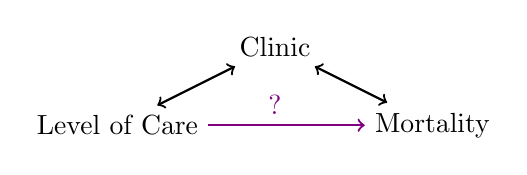
\begin{tikzpicture}[thick]
                        \node (1) at (0,1) {Clinic};
                        \node (2) at (-2,0) {Level of Care};
                        \node (3) at (2,0) {Mortality};
                        \draw[<->] (1) to (2);
                        \draw[<->] (1) to (3);
                        \draw[->,Purple] (2) to (3) node[anchor=south,midway] {$?$};
                  \end{tikzpicture}
            \end{figure}
      \item Instead of having to examine multiple $ 2\times 2 $ tables we'd like to estimate the $ \OR $
            and compute associations using a multiple regression model.
      \item One way to do this is by fitting a Binomial GLM to the data.
\end{itemize}
% Week 4

\makeheading{Week 4}{\daterange{2021-09-27}{2021-10-01}}
\section*{Topic 3b: Binomial Regression Models for Binary Data}
\addcontentsline{toc}{section}{Topic 3b: Binomial Regression Models for Binary Data}
\subsection*{Recall Topic 3a: Binary Data and Odds Ratios}
Last week, we introduce a simple method for association between two binary
variables, \textcolor{Blue}{$ 2\times 2 $ contingency table analysis}:
\begin{table}[!htbp]
      \centering
      \begin{NiceTabular}{l|ccc}
            & \multicolumn{2}{c}{\emph{Mortality}}                                                 \\
            Level of Care & Died                            & Survived                                 \\
            \cmidrule{1-3}
            Intensive & $ y_1 $                            & $ m_1-y_1 $    & $ Y_1 \sim \BIN{m_1,\pi_1} $         \\
            Regular   & $ y_2 $                            & $ m_2-y_2 $    & $ Y_2 \sim \BIN{m_2,\pi_2} $      \\
            \cmidrule{1-3}
      \end{NiceTabular}
\end{table}
Measure of Association: $ \displaystyle \OR = \psi=\frac{\pi_1/(1-\pi_1)}{\pi_2/(1-\pi_2)} $,
\begin{itemize}
      \item $ \OR=1 $ (equal risk).
      \item $ 0<\OR<1 $ (lower risk in group 1).
      \item $ \OR>1 $ (higher risk in group 1).
\end{itemize}
Maximum likelihood estimator for $ \OR $ is:
\[ \hat{\psi}=\frac{y_1/(m_1-y_1)}{y_2/(m_2-y_2)}, \]
and a Wald-based \qty{95}{\percent} CI is:
\[ \exp[\bigg]{\log{\hat{\psi}_1}\pm 1.96\underbrace{\sqrt{\frac{1}{y_1} +\frac{1}{m_1-y_1} +\frac{1}{y_2} +\frac{1}{m_2-y_2}}}_{\se{\log{\hat{\psi}}}}}. \]
\subsection*{Prenatal Care Data Example}
\begin{table}[!htbp]
      \centering
      \begin{tabular}{ccc}
            OR (\textcolor{Blue}{Mortality and Care}) & Est.                   & \qty{95}{\percent} CI             \\
            \midrule
            Intensive vs Regular                      & \textcolor{Blue}{0.51} & \textcolor{Blue}{$ (0.30,0.89) $} \\
            \bottomrule
      \end{tabular}
      \caption{$ 1\notin (0.30,0.89)\implies $ evidence of association between Mortality and Care.}
\end{table}

However, Mortality and Care are also related to another variable, Clinic:
\begin{table}[!htbp]
      \centering
      \begin{tabular}{ccc}
            OR (\textcolor{Blue}{Mortality and Clinic}) & Est.                   & \qty{95}{\percent} CI             \\
            \midrule
            Clinic A vs Clinic B                        & \textcolor{Blue}{0.35} & \textcolor{Blue}{$ (0.12,0.58) $} \\
            \bottomrule
      \end{tabular}
      \caption{Association between Mortality and Clinic.}
\end{table}
\begin{table}[!htbp]
      \centering
      \begin{tabular}{ccc}
            OR (\textcolor{Blue}{Care and Clinic}) & Est.                    & \qty{95}{\percent} CI              \\
            \midrule
            Clinic A vs Clinic B                   & \textcolor{Blue}{14.06} & \textcolor{Blue}{$ (9.12,21.76) $} \\
            \bottomrule
      \end{tabular}
      \caption{Association between Care and Clinic.}
\end{table}
\begin{itemize}
      \item Therefore, we wish to consider how a variable, e.g., Mortality ($ Y $), is related to
            multiple explanatory variables together, e.g., Care ($ x_1 $) and Clinic ($ x_2 $).
      \item This can be done using \textcolor{Blue}{multiple regression methodology} for binary data $ \implies $
            Topic 3b: Binomial Regression Models for Binary Data.
\end{itemize}
\subsection*{Multiple Regression for Binary Data}
\begin{itemize}
      \item Often we need to consider the relationship between a binary outcome and
            multiple explanatory variables, using multiple regression methodology.
      \item This is because we may want to:
            \begin{itemize}
                  \item control for cofounding variables and hence want to examine the effect of
                        several variables simultaneously;
                  \item examine the effect of categorical variables ($ >2 $ levels) or continuous covariates;
                  \item develop sophisticated models that describe complex relationship.
            \end{itemize}
      \item Suppose \textcolor{Blue}{\emph{subject level data}} is binary with a value of 1 indicating that an event
            of interest occurs and a value of 0 indicating that event doesn't occur.
      \item Subjects can be classified according to the values of explanatory
            variables into $n$ groups (i.e., common covariates values within each group), so
            we have \textcolor{Blue}{\emph{grouped data}} such that:
            \begin{itemize}
                  \item $ m_i $ denotes number of subjects in group $i$;
                  \item $Y_i$ denotes number of subjects experienced the event in group $i$;
                  \item $ x_{i1},\ldots,x_{ip} $ denote the covariates values associated with group $i$
                        where $ i=1,\ldots,n $.
            \end{itemize}
\end{itemize}
\subsection*{Set-up of a Binomial Regression Model}
\begin{enumerate}[label=\color{Blue}\protect\circled{\arabic*}]
      \item \textcolor{Blue}{Response Variable}: $ Y_i \sim \BIN{m_i,\pi_i} $, $ i=1,\ldots,n $, and Binomial
            distribution is a member of Exponential family!
            \begin{align*}
                  f(y_i)
                   & =\binom{m_i}{y_i}\pi_i^{y_i}(1-\pi_i)^{m_i-y_i}                                   \\
                   & =\exp*{y_i\log*{\frac{\pi_i}{1-\pi_i}}+m_i\log{1-\pi_i}+\log*{\binom{m_i}{y_i}}},
            \end{align*}
            where
            \begin{align*}
                  \theta_i     & =\log*{\frac{\pi_i}{1-\pi_i}},                       \\
                  a(\phi)=\phi & =1,                                                  \\
                  b(\theta_i)  & =-m_i\log{1-\pi_i}=m_i\log{1+\mathrm{e}^{\theta_i}}. \\
                  c(y_i;\phi)  & =\log*{\binom{m_i}{y_i}}.
            \end{align*}
      \item \textcolor{Blue}{Linear Predictor}:
            \[ \eta_i=\Vector{x}_i^\top \Vector{\beta}=\beta_0+\beta_1x_{i1}+\cdots+\beta_p x_{ip}. \]
      \item \textcolor{Blue}{Link Function}: Recall that for Binomial distribution, we have $ \E{Y_i}=\mu_i=m_i\pi_i $,
            therefore we typically re-write the link function in terms of $ \pi_i $,
            \[ \textcolor{Blue}{g(\pi_i)}=\Vector{x}_i^\top \Vector{\beta}. \]
            As $ \pi_i\in(0,1) $, any function $ g\colon (0,1)\to(-\infty,\infty) $ may work, and here are some link functions we
            can consider:
            \begin{table}[!htbp]
                  \centering
                  \begin{tabular}{cc}
                        \toprule
                        log-log                             & $ g(\pi)=\log[\big]{-\log{\pi}} $                                               \\
                        complementary log-log               & $ g(\pi)=\log[\big]{-\log{1-\pi}} $                                             \\
                        Probit$^a$                          & $ g(\pi)=\Phi^{-1}(\pi) $                                                       \\
                        Logit (\textcolor{Blue}{canonical}) & $ g(\pi)=\log[\big]{\pi/(1-\pi)} $                                              \\
                        \bottomrule
                        \multicolumn{2}{l}{\footnotesize{$ {}^a $For the Probit link, $ \Phi(\:\cdot\:) $ is the \emph{CDF} of $ \N{0,1} $.}} \\
                  \end{tabular}
            \end{table}
\end{enumerate}
\subsection*{Canonical Link and Logistic Regression}
Recall for Binomial distribution $ \theta_i=\log*{\frac{\pi_i}{1-\pi_i} } $, and by setting $ \theta_i=\eta_i $, we have:
\[ \log*{\frac{\pi_i}{1-\pi_i}}=\eta_i. \]
The \textcolor{Blue}{Logit link}, $ g(\pi_i)=\log[\big]{\pi_i/(1-\pi_i)} $, is the canonical link for the Binomial!
% \begin{noindent}
\begin{knitrout}
\definecolor{shadecolor}{rgb}{0.969, 0.969, 0.969}\color{fgcolor}

{\centering \includegraphics[width=\maxwidth]{figure/unnamed-chunk-31-1} 

}


\end{knitrout}
% \end{noindent}
This leads to a Logistic Regression Model:
\[ \log*{\frac{\pi_i}{1-\pi_i}}=\Vector{x}_i^\top \Vector{\beta}=\beta_0+\beta_1x_{i1}+\cdots+\beta_p x_{ip}. \]
\subsection*{Prediction from Logistic Regression}
Aside: The inverse of the logit function is called the expit function:
\[ \logit{\pi_i}=\log*{\frac{\pi_i}{1-\pi_i}}=\Vector{x}_i^\top \Vector{\beta}\iff \pi_i=\frac{\exp{\Vector{x}_i^\top \Vector{\beta}}}{1+\exp{\Vector{x}_i^\top \Vector{\beta}}}=\expit{\Vector{x}_i^\top \Vector{\beta}}.  \]
Suppose we have found MLE $ \hat{\Vector{\beta}} $ using Fisher scoring, then the fitted value for the \textcolor{Blue}{probability of response} $ \pi_i $ given explanatory
variables $ \Vector{x}_i $ is:
\[ \hat{\pi}_i=\frac{\exp{\Vector{x}_i^\top \hat{\Vector{\beta}}}}{1+\exp{\Vector{x}_i^\top \hat{\Vector{\beta}}}}. \]
The predicted number of responses are: $ \hat{Y}_i=m_i\hat{\pi}_i $.

\subsection*{Interpretation of $ \Vector{\beta} $ in Logistic Regression}
\begin{itemize}
      \item Consider a simple logistic model with a single binary explanatory variable:
            \[ \log*{\frac{\pi_i}{1-\pi_i}}=\beta_0+\beta_1x_{i1}, \]
            where $ x_{i1}=0 $ (group 0) and $ x_{i1}=1 $ (group 1).
      \item Let's compare the model when $ x_{i1}=1 $ vs $ x_{i1}=0 $.
            \begin{table}[!htbp]
                  \centering
                  \begin{tabular}{ccrl}
                        Group & $ \Vector{x}_i^\top $ & $ \eta_i $          & $ =\log[\big]{\pi_i/(1-\pi_i)} $                              \\
                        \midrule
                        1     & $ (1,1)^\top $        & $ \beta_0+\beta_1 $ & $ =\log[\big]{\pi_1/(1-\pi_1)} $                              \\
                        0     & $ (1,0)^\top $        & $ \beta_0 $         & $ =\log[\big]{\pi_0/(1-\pi_0)} $                              \\
                        \midrule
                              &                       & $ \beta_1 $         & $ =\log*{\frac{\pi_1/(1-\pi_1)}{\pi_0/(1-\pi_0)}}=\log{\OR} $
                  \end{tabular}
            \end{table}
      \item We subtract line 2 from line 1 to isolate $ \beta_1 $ and find its interpretation.
      \item $ \beta_1= $ log odds ratio of response for subjects with $ x_{i1}=1 $ vs $ x_{i1}=0 $.
      \item Please see Section 2.4.2 for general interpretations of $ \Vector{\beta} $'s in multiple logistic regression models.
\end{itemize}
\subsection*{Logistic Regression for Prenatal Care Example}
\begin{itemize}
      \item \textcolor{Blue}{Response}: Fetal Mortality, that is,
            \[ Y_i \sim \BIN{m_i,\pi_i},\; i=1,2,\ldots. \]
      \item Explanatory Variables:
            \begin{align*}
                  x_{i1} & =\begin{cases*}
                                  1 & Intensive Care \\
                                  0 & Regular Care
                            \end{cases*}                           \\
                  x_{i2} & =\begin{cases*}
                                  1 & Clinic A \\
                                  0 & Clinic B \\
                            \end{cases*}                                \\
                  x_{i3} & =x_{i1}x_{i2}=\begin{cases*}
                                               1 & Intensive care and Clinic A \\
                                               0 & Otherwise
                                         \end{cases*}
            \end{align*}
      \item We will use the context of this example to illustrate how to:
            \begin{itemize}
                  \item fit (simple and multiple) logistic regression models using R, and
                  \item interpret regression parameters.
            \end{itemize}
\end{itemize}
\subsection*{Model 1: Level of Care only model}
\[ \log*{\frac{\pi_i}{1-\pi_i}}=\beta_0+\beta_1x_{i1}. \]
\begin{table}[!htbp]
      \centering
      \begin{tabular}{cccl}
            Level of Care & Clinic & $ \Vector{x}_i^\top $ & $ \log[\big]{\pi_i/(1-\pi_i)} $ \\
            \midrule
            Intensive     & ---    & $ (1,1)^\top $        & $ \beta_0+\beta_1 $             \\
            Regular       & ---    & $ (1,0)^\top $        & $ \beta_0 $                     \\
            \bottomrule
      \end{tabular}
\end{table}
\begin{itemize}
      \item $ \beta_0= $ \textcolor{Blue}{log odds} of mortality for babies born to mothers treated with regular care.
      \item $ \beta_1= $ \textcolor{Blue}{log odds ratio} of mortality for babies born to mothers treated
            with intensive vs regular care.
\end{itemize}
\subsection*{Model 2: Main effects model}
\[ \log*{\frac{\pi_i}{1-\pi_i}}=\beta_0+\beta_1x_{i1}+\beta_2x_{i2}. \]
\begin{table}[!htbp]
      \centering
      \begin{tabular}{cccl}
            Level of Care & Clinic & $ \Vector{x}_i^\top $ & $ \log[\big]{\pi_i/(1-\pi_i)} $ \\
            \midrule
            Intensive     & A      & $ (1,1,1)^\top $      & $ \beta_0+\beta_1+\beta_2 $     \\
            Regular       & A      & $ (1,0,1)^\top $      & $ \beta_0+\beta_2 $             \\
            Intensive     & B      & $ (1,1,0)^\top $      & $ \beta_0+\beta_1 $             \\
            Regular       & B      & $ (1,0,0)^\top $      & $ \beta_0 $                     \\
            \bottomrule
      \end{tabular}
\end{table}
\begin{itemize}
      \item $ \beta_0= $ \textcolor{Blue}{log odds} of mortality with regular care at Clinic B.
      \item $ \beta_1= $ \textcolor{Blue}{log odds ratio} of mortality for babies born to mothers treated with
            \textcolor{Blue}{intensity vs regular} care at the \emph{same clinic}.
      \item $ \beta_2= $ \textcolor{Blue}{log odds ratio} of mortality for babies born to mothers treated at
            \textcolor{Blue}{Clinic A vs Clinic B} at the \emph{same level of care}.
\end{itemize}
\subsection*{Model 3: Interaction model}
\[ \log*{\frac{\pi_i}{1-\pi_i}}=\beta_0+\beta_1x_{i1}+\beta_2x_{i2}+\beta_3x_{i3}. \]
\begin{table}[!htbp]
      \centering
      \begin{tabular}{cccl}
            Level of Care & Clinic & $ \Vector{x}_i^\top $ & $ \log[\big]{\pi_i/(1-\pi_i)} $     \\
            \midrule
            Intensive     & A      & $ (1,1,1)^\top $      & $ \beta_0+\beta_1+\beta_2+\beta_3 $ \\
            Regular       & A      & $ (1,0,1)^\top $      & $ \beta_0+\beta_2 $                 \\
            Intensive     & B      & $ (1,1,0)^\top $      & $ \beta_0+\beta_1 $                 \\
            Regular       & B      & $ (1,0,0)^\top $      & $ \beta_0 $                         \\
            \bottomrule
      \end{tabular}
\end{table}
\begin{itemize}
      \item $ \beta_1= $ \textcolor{Blue}{log odds ratio} of mortality for babies born to mothers treated with
            \textcolor{Blue}{intensity vs regular} care at \emph{Clinic B}.
      \item $ \beta_1+\beta_3= $ \textcolor{Blue}{log odds ratio} of mortality for babies born to mothers treated
            with \textcolor{Blue}{intensity vs regular} care at \emph{Clinic A}.
      \item $ \beta_2= $ \textcolor{Blue}{log odds ratio} of mortality for babies born to mothers treated at
            \textcolor{Blue}{Clinic A vs Clinic B} with \emph{regular} care.
      \item $ \beta_2+\beta_3= $ \textcolor{Blue}{log odds ratio} of mortality for babies born to mothers treated at
            \textcolor{Blue}{Clinic A vs Clinic B} with \emph{intensive} care.
      \item $ \beta_3 $ represents the \textcolor{Blue}{difference in log odds ratios}.
      \item If $ \beta_3=0 $ then association between mortality and level of care does not
            dependent on clinic.
      \item Equivalently, if $ \beta_3=0 $ then the association between mortality and clinic
            does not depend on level of care.
\end{itemize}
\begin{Example}{Data file \texttt{prenatal.dat}}
\begin{knitrout}
\definecolor{shadecolor}{rgb}{0.969, 0.969, 0.969}\color{fgcolor}\begin{kframe}
\begin{verbatim}
  clinic loc  y   m
1      0   0 34 231
2      0   1  4  27
3      1   0 12 188
4      1   1 16 309
\end{verbatim}
\end{kframe}
\end{knitrout}
      \begin{itemize}
            \item The first line contains the variable names/labels.
            \item We are using indicator variables for the explanatory variables:
                  \begin{align*}
                        x_{i1} & =\text{\texttt{loc}}    &  & \text{(1 for Intensive, 0 for Regular)} \\
                        x_{i2} & =\text{\texttt{clinic}} &  & \text{(1 for Clinic A, 0 for Clinic B)}
                  \end{align*}
            \item The variable \texttt{y} records the number of deaths (events).
      \end{itemize}
\end{Example}
\subsection*{Fit GLMs using R}
The \texttt{glm()} function in R is used to fit the generalized linear models:
\[ \text{\texttt{fit = glm(formula, family = (link = ), data = )}}. \]
\begin{itemize}
      \item \texttt{formula}: a linear formula describing the model, e.g.,
            \[ \texttt{resp \textasciitilde{} loc + clinic}. \]
      \item \texttt{family}: a description of the exponential family distribution and link
            function to be used in the model, e.g.,
            \[ \text{\texttt{family = binomial, gaussian, poisson, Gamma, etc.}}. \]
            \[ \text{\texttt{link = logit, log, loglog, cloglog, identity, probit, etc.}}. \]
      \item The default is the canonical link.
\end{itemize}
\subsection*{R Code and Output for Analysis of Prenatal Care data}
For binomial data, we need to construct ``\texttt{resp}'' variable as the pair $ (y_i,m_i-y_i) $.
% \begin{noindent}
\begin{knitrout}
\definecolor{shadecolor}{rgb}{0.969, 0.969, 0.969}\color{fgcolor}\begin{kframe}
\begin{alltt}
\hlcom{# read file prenatal.data}
\hlstd{prenatal.dat} \hlkwb{=} \hlkwd{read.table}\hlstd{(}\hlstr{"prenatal.dat"}\hlstd{,} \hlkwc{header} \hlstd{= T)}
\hlcom{# construct the binomial response for the logistic regression}
\hlcom{# analysis}
\hlstd{prenatal.dat}\hlopt{$}\hlstd{resp} \hlkwb{=} \hlkwd{cbind}\hlstd{(prenatal.dat}\hlopt{$}\hlstd{y, prenatal.dat}\hlopt{$}\hlstd{m} \hlopt{-} \hlstd{prenatal.dat}\hlopt{$}\hlstd{y)}
\hlstd{prenatal.dat}
\end{alltt}
\begin{verbatim}
  clinic loc  y   m resp.1 resp.2
1      0   0 34 231     34    197
2      0   1  4  27      4     23
3      1   0 12 188     12    176
4      1   1 16 309     16    293
\end{verbatim}
\end{kframe}
\end{knitrout}
% \end{noindent}
The logistic regression models are fit using the \texttt{glm()} commands like:
% \begin{noindent}
\begin{knitrout}
\definecolor{shadecolor}{rgb}{0.969, 0.969, 0.969}\color{fgcolor}\begin{kframe}
\begin{alltt}
\hlcom{# fit the logistic model using the glm function}
\hlstd{model1} \hlkwb{=} \hlkwd{glm}\hlstd{(resp} \hlopt{~} \hlstd{loc,} \hlkwc{family} \hlstd{=} \hlkwd{binomial}\hlstd{(}\hlkwc{link} \hlstd{= logit),} \hlkwc{data} \hlstd{= prenatal.dat)}
\hlkwd{summary}\hlstd{(model1)}
\end{alltt}
\end{kframe}
\end{knitrout}
% \end{noindent}
\subsection*{Fit of Model 1: Level of Care Model}
\[ \log*{\frac{\pi_i}{1-\pi_i}}=\beta_0+\beta_1x_{i1}. \]
% \begin{noindent}
\begin{knitrout}
\definecolor{shadecolor}{rgb}{0.969, 0.969, 0.969}\color{fgcolor}\begin{kframe}
\begin{alltt}
\hlcom{# fit the logistic model using the glm function}
\hlstd{model1} \hlkwb{=} \hlkwd{glm}\hlstd{(resp} \hlopt{~} \hlstd{loc,} \hlkwc{family} \hlstd{=} \hlkwd{binomial}\hlstd{(}\hlkwc{link} \hlstd{= logit),} \hlkwc{data} \hlstd{= prenatal.dat)}
\hlkwd{summary}\hlstd{(model1)}\hlopt{$}\hlstd{coefficients}
\end{alltt}
\begin{verbatim}
              Estimate Std. Error    z value     Pr(>|z|)
(Intercept) -2.0929370  0.1562692 -13.393150 6.630754e-41
loc         -0.6670729  0.2785400  -2.394891 1.662530e-02
\end{verbatim}
\end{kframe}
\end{knitrout}
% \end{noindent}
Components of the \texttt{summary()} output for \texttt{glm} objects:
\begin{itemize}
      \item \textcolor{Blue}{\texttt{Estimate}}: the maximum likelihood estimates of the regression coefficients $ \hat{\beta}_0 $
            and $ \hat{\beta}_1 $.
      \item \textcolor{Blue}{\texttt{Std.\ Error}}: estimated standard errors, the square root of the diagonal
            of the inverse of the Information matrix:
            \[ \se{\hat{\beta}_j}=\sqrt{\bigl[\Matrix{I}^{-1}(\hat{\Vector{\beta}})\bigr]_{jj}}=\sqrt{I^{jj}(\hat{\Vector{\beta}})}. \]
      \item \textcolor{Blue}{\texttt{z value}}: Wald-type test statistics for testing the hypotheses:
            \begin{center}
                  $ \HN $: $ \beta_j=0 $ vs $ \HA $: $ \beta_j\ne 0 $.
            \end{center}
      \item \textcolor{Blue}{\texttt{Pr(>|z|)}}: $ p $-value for above Wald test.
\end{itemize}
For this model:
\begin{itemize}
      \item $ \beta_1 $ is the log odds ratio of mortality for infants born to mothers treated
            with intensive versus regular care.
\end{itemize}
\subsection*{Hypothesis test for $ \beta_j $}
\begin{itemize}
      \item We may wish to test:
            \begin{center}
                  $ \HN $: $ \beta_j=\beta^\star $ versus $ \HA $: $ \beta_j\ne \beta^\star $.
            \end{center}
      \item The general \textcolor{Blue}{Wald} result for a single parameter $ \beta_j $ is:
            \[ (\hat{\beta}_j-\beta^\star)^2\bigl(I^{jj}(\hat{\Vector{\beta}})\bigr)^{-1} \sim \chi^2_1, \]
            equivalently
            $ \displaystyle \frac{\hat{\beta}_j-\beta^\star}{\se{\hat{\beta}_j}}\sim \N{0,1} $
            where $ \se{\hat{\beta}_j}=\sqrt{I^{jj}(\hat{\Vector{\beta}})} $.
      \item We can find the $ p $-value of this test using:
            \[ p=2\Prob*{Z>\frac{\abs{\hat{\beta}_j-\beta^\star}}{\se{\hat{\beta}_j}}}. \]
      \item The \texttt{summary()} output gives the test statistics and $p$-values for testing
            \begin{center}
                  $ \HN $: $ \beta_j=0 $ vs $ \HA $: $ \beta_j\ne 0 $.
            \end{center}
\end{itemize}
\subsection*{Hypothesis test for $ \beta_1 $ from Model 1: Level of Care Model}
% \begin{noindent}
\begin{knitrout}
\definecolor{shadecolor}{rgb}{0.969, 0.969, 0.969}\color{fgcolor}\begin{kframe}
\begin{alltt}
\hlkwd{summary}\hlstd{(model1)}\hlopt{$}\hlstd{coefficients}
\end{alltt}
\begin{verbatim}
              Estimate Std. Error    z value     Pr(>|z|)
(Intercept) -2.0929370  0.1562692 -13.393150 6.630754e-41
loc         -0.6670729  0.2785400  -2.394891 1.662530e-02
\end{verbatim}
\end{kframe}
\end{knitrout}
% \end{noindent}
\begin{itemize}
      \item We wish to test:
            \begin{center}
                  $ \HN $: $ \beta_1=0 $ vs $ \HA $: $ \beta_1\ne 0 $
            \end{center}
      \item Wald test:
            \[ z=\frac{\hat{\beta}_1-0}{\se{\hat{\beta}_1}}=\frac{-0.6671}{0.2785}=-2.3949   \]
      \item $ p $-value:
            \[ p=2\Prob{Z>\abs{-2.3949}}=0.0166<0.05 \]
      \item Therefore, we reject the null hypothesis that $ \beta_1=0 $.
\end{itemize}
\begin{itemize}
      \item Estimate of $ \OR $ for Mortality for Intensive vs Regular Care:
            \[ \hat{\psi}=\exp{\hat{\beta}_1}=\exp{-0.6670729}=0.51. \]
      \item Confidence Interval for OR:
            \begin{align*}
                  \exp[\big]{\hat{\beta}_1\pm 1.96\se{\hat{\beta}_1}}
                   & =\exp{-0.6671\pm 1.96(0.2785)} \\
                   & =(\exp{-1.2130},\exp{-0.1211}) \\
                   & =(0.30,0.89)
            \end{align*}
      \item The estimate and Wald \qty{95}{\percent} CI here match those found previously from
            the $ 2\times 2 $ table analysis. That is, the $ 2\times 2 $ table analysis is equivalent to
            a simple logistic regression with a single binary covariate.
\end{itemize}
\subsection*{Fit of Model 2: Main Effects Model}
\[ \log*{\frac{\pi_i}{1-\pi_i}}=\beta_0+\beta_1x_{i1}+\textcolor{Blue}{\beta_2x_{i2}}. \]
% \begin{noindent}
\begin{knitrout}
\definecolor{shadecolor}{rgb}{0.969, 0.969, 0.969}\color{fgcolor}\begin{kframe}
\begin{alltt}
\hlstd{model2} \hlkwb{<-} \hlkwd{glm}\hlstd{(resp} \hlopt{~} \hlstd{loc} \hlopt{+} \hlstd{clinic,} \hlkwc{family} \hlstd{=} \hlkwd{binomial}\hlstd{(}\hlkwc{link} \hlstd{= logit),} \hlkwc{data} \hlstd{= prenatal.dat)}
\hlkwd{summary}\hlstd{(model2)}\hlopt{$}\hlstd{coefficients}
\end{alltt}
\begin{verbatim}
              Estimate Std. Error    z value     Pr(>|z|)
(Intercept) -1.7410476  0.1784691 -9.7554560 1.748132e-22
loc         -0.1503053  0.3301670 -0.4552402 6.489365e-01
clinic      -0.9862793  0.3089322 -3.1925427 1.410261e-03
\end{verbatim}
\end{kframe}
\end{knitrout}
% \end{noindent}
\begin{itemize}
      \item What is the OR for mortality for Intensive vs Regular Care, now controlling for
            Clinic?
            \[ \widehat{\OR}=\hat{\psi}=\exp{-0.1503}=0.86. \]
      \item \qty{95}{\percent} CI:
            \[ \exp{-0.1503\pm 1.96\times 0.3302}=(0.4505,1.6436). \]
\end{itemize}
\subsection*{Fit of Model 3: Interaction Model}
\[ \log*{\frac{\pi_i}{1-\pi_i}}=\beta_0+\beta_1x_{i1}+\beta_2x_{i2}+\textcolor{Blue}{\beta_3x_{i3}}. \]
% \begin{noindent}
\begin{knitrout}
\definecolor{shadecolor}{rgb}{0.969, 0.969, 0.969}\color{fgcolor}\begin{kframe}
\begin{alltt}
\hlstd{model3} \hlkwb{<-} \hlkwd{glm}\hlstd{(resp} \hlopt{~} \hlstd{loc} \hlopt{+} \hlstd{clinic} \hlopt{+} \hlstd{loc} \hlopt{*} \hlstd{clinic,} \hlkwc{family} \hlstd{=} \hlkwd{binomial}\hlstd{(}\hlkwc{link} \hlstd{= logit),}
  \hlkwc{data} \hlstd{= prenatal.dat)}
\hlkwd{summary}\hlstd{(model3)}\hlopt{$}\hlstd{coefficients}
\end{alltt}
\begin{verbatim}
                Estimate Std. Error     z value     Pr(>|z|)
(Intercept) -1.756843204  0.1857092 -9.46018403 3.074017e-21
loc          0.007643349  0.5726827  0.01334657 9.893513e-01
clinic      -0.928734141  0.3514300 -2.64272868 8.224091e-03
loc:clinic  -0.229649891  0.6949054 -0.33047646 7.410400e-01
\end{verbatim}
\end{kframe}
\end{knitrout}
% \end{noindent}
\begin{table}[!htbp]
      \centering
      \begin{tabular}{cccl}
            Level of Care & Clinic & $ \Vector{x}_i^\top $ & $ \log[\big]{\pi_i/(1-\pi_i)} $     \\
            \midrule
            Intensive     & A      & $ (1,1,1)^\top $      & $ \beta_0+\beta_1+\beta_2+\beta_3 $ \\
            Regular       & A      & $ (1,0,1)^\top $      & $ \beta_0+\beta_2 $                 \\
            Intensive     & B      & $ (1,1,0)^\top $      & $ \beta_0+\beta_1 $                 \\
            Regular       & B      & $ (1,0,0)^\top $      & $ \beta_0 $                         \\
            \bottomrule
      \end{tabular}
\end{table}
\begin{itemize}
      \item What is the OR for Mortality for Intensive vs Regular Care at Clinic A?
            \[ \OR=\psi=\exp{\beta_1+\beta_3}\implies \hat{\psi}=\exp{0.0076-0.2296}=0.8. \]
      \item $ \se{\hat{\beta}_1+\hat{\beta}_3} $ is required for calculation of \qty{95}{\percent} CI.
            \begin{itemize}
                  \item Recall $ \Var{\hat{\beta}}=\Matrix{I}^{-1}(\hat{\Vector{\beta}}) $, now for any linear function of $ \Vector{\beta} $'s,
                        e.g., $ \Vector{c}\Vector{\beta} $ where $ \Vector{c} $ is a row vector of constants, then MLE of $ \Vector{c}\Vector{\beta} $
                        is $ \Vector{c}\hat{\Vector{\beta}} $, and $ \se{\hat{\Vector{c}\hat{\Vector{\beta}}}}=\sqrt{\Vector{c}\Matrix{I}^{-1}(\hat{\Vector{\beta}})\Vector{c}^\top} $.
            \end{itemize}
      \item Therefore, $ \log{\psi}=\beta_1+\beta_3=\Vector{c}\Vector{\beta} $, $ \Vector{c}=(0,1,0,1) $. In R, \texttt{vcov(model3)}
            gives $ \Matrix{I}^{-1}(\hat{\Vector{\beta}}) $.
      \item What is OR for Mortality for Intensive vs Regular Care at Clinic B?
            \[ \OR=\psi=\exp{\beta_1}\implies \hat{\psi}=\exp{0.0076}=1.01. \]
\end{itemize}

\section*{Topic 3c: Likelihood Ratio Test for Logistic Regression Models}
\addcontentsline{toc}{section}{Topic 3c: Likelihood Ratio Test for Logistic Regression Models}
\subsection*{Logistic Regression Models}
Recall major developments of Binomial logistic regression from last topic 3b: $ Y_i \sim \BIN{m_i,\pi_i} $,
$ i=1,\ldots,n $ independently, with covariate vector $ \Vector{x}_i $ and
\[ \textcolor{Blue}{\log*{\frac{\pi_i}{1-\pi_i}}}=\Vector{x}_i^\top \Vector{\beta}. \]
\begin{itemize}
      \item Estimation: $ \hat{\Vector{\beta}} $ come from Fisher scoring using R function \texttt{glm()}.
      \item Interpretation: $ \exp{\beta_j} $ has $ \OR $ interpretation.
      \item Hypothesis tests of $ \HN $: $ \beta_j=0 $ using Wald statistic.
      \item Confidence Intervals: $ \hat{\beta}_j\pm z_{1-\alpha/2}\se{\hat{\beta}_j} $.
\end{itemize}
\subsection*{Likelihood for Logistic Regression Models}
\begin{itemize}
      \item Log-likelihood for Binomial Distribution:
            \begin{align*}
                  \ell
                   & =\log[\bigg]{\prod_{i=1}^n \pi_i^{y_i}(1-\pi_i)^{m_i-y_i}}        \\
                   & =\sum_{i=1}^{n} y_i\log*{\frac{\pi_i}{1-\pi_i}}+m_i\log{1-\pi_i}.
            \end{align*}
      \item Using logit link we can re-parameterize the log-likelihood in terms of $ \Vector{\beta} $:
            \[ \log*{\frac{\pi_i}{1-\pi_i}}=\Vector{x}_i^\top \Vector{\beta},\qquad \pi_i=\frac{\exp{\Vector{x}_i^\top \Vector{\beta}}}{1+\exp{\Vector{x}_i^\top \Vector{\beta}}}. \]
      \item Log likelihood for logistic regression:
            \[ \ell=\sum_{i=1}^{n} y_i\Vector{x}_i^\top \Vector{\beta}-m_i\log[\big]{1+\exp{\Vector{x}_i^\top \Vector{\beta}}}. \]
      \item Maximization of log-likelihood $ \ell(\Vector{\beta}) $ gives MLE $ \hat{\Vector{\beta}} $, and
            \begin{itemize}
                  \item estimated probability of response:
                        \[ \hat{\pi}_i=\mathrm{e}^{\Vector{x}_i^\top \hat{\Vector{\beta}}}/(1+\mathrm{e}^{\Vector{x}_i^\top \hat{\Vector{\beta}}})=\expit{\Vector{x}_i^\top \hat{\Vector{\beta}}}, \]
                  \item estimated number of responses: $ \hat{y}_i=m_i\hat{\pi}_i $.
            \end{itemize}
      \item Questions:
            \begin{itemize}
                  \item How good is the model? How well do the estimated number of events $ \hat{y}_i $ approximate the observed data $ y_i $? (\textcolor{Red}{goodness of fit}).
                  \item How much worse is the fit of a model when several of the covariates are excluded? (\textcolor{Red}{nested models}):
                        \begin{center}
                              $ \HN $: $ \beta_k=\beta_{k+1}=0 $ vs $ \HA $: $ \beta_k\ne 0 $ or $ \beta_{k+1}\ne 0 $.
                        \end{center}
            \end{itemize}
\end{itemize}
\subsection*{Likelihood Ratio Test (General Setting)}
\begin{itemize}
      \item Suppose $ \ell(\Vector{\theta}) $ is the likelihood for a $ q $-dimension parameter vector $ \Vector{\theta} $ and let
            \begin{itemize}
                  \item $ \tilde{\Vector{\theta}} $ be the $ q $-dim MLE of $ \Vector{\theta} $ (unconstrained/\textcolor{Blue}{saturated, $ q=n $}),
                  \item $ \hat{\Vector{\theta}} $ be the $ p $-dim MLE of $ \Vector{\theta} $ (constrained/\textcolor{Blue}{unsaturated, $ p<q $}).
            \end{itemize}
      \item Hypotheses:
            \begin{itemize}
                  \item $ \HN $: the constrained model is adequate (i.e., as good as the unconstrained).
                  \item $ \HA $: constrained model is not adequate.
            \end{itemize}
      \item Recall the Likelihood Ratio (LR) result:
            \[ \text{Under $ \HN $:}\quad -2\log*{\frac{L(\hat{\Vector{\theta}})}{L(\tilde{\Vector{\theta}})}}
                  =-2\bigl[\ell(\hat{\Vector{\theta}})-\ell(\tilde{\Vector{\theta}})\bigr]\sim \chi^2_{q-p}. \]
      \item Reject $ \HN $ at $ \theta $ if
            \[ p\text{-value}=\Prob[\Big]{\chi^2_{q-p}>-2\bigl[\ell(\hat{\Vector{\theta}})-\ell(\tilde{\Vector{\theta}})\bigr]}<\alpha. \]
\end{itemize}
\subsection*{Likelihood Ratio Test (Logistic Regression Model)}
\begin{itemize}
      \item \textcolor{Blue}{Saturated} (unconstrained) model MLEs:
            \[ \textcolor{Red}{\tilde{\pi}_i=\frac{y_i}{m_i}},\; i=1,\ldots,n. \]
            \begin{itemize}
                  \item Binomial MLE without imposing any constraint.
                  \item We will have $ \tilde{y}_i=m_i\tilde{\pi}_i=y_i $, \textcolor{Blue}{a perfect fit}!
            \end{itemize}
      \item \textcolor{Blue}{Unsaturated} (constrained) model MLEs:
            \[ \textcolor{Red}{\hat{\pi}_i=\expit{\Vector{x}_i^\top \hat{\Vector{\beta}}}}. \]
            \begin{itemize}
                  \item Regression models are a way of imposing constraints on the estimation of $ \pi_i $ through $ p $-dim regression coefficients $ \Vector{\beta} $.
                  \item We will have fitted number of responses $ \hat{y}_i=m_i\hat{\pi}_i=m_i\expit{\Vector{x}_i^\top \hat{\Vector{\beta}}} $.
            \end{itemize}
      \item \textcolor{Blue}{Hypotheses}:
            \begin{itemize}
                  \item $ \HN $: the $ p $-dim model, e.g., $ \logit{\pi_i}=\Vector{x}_i^\top \Vector{\beta} $ is adequate.
                  \item $ \HA $: the $ p $-dim model, e.g., $ \logit{\pi_i}=\Vector{x}_i^\top \Vector{\beta} $ is not adequate \emph{compared
                              to the $ n $-dim saturated model}.
            \end{itemize}
      \item \textcolor{Blue}{Likelihood Ratio Statistic} (also referred to as the \textcolor{Blue}{Deviance}):
            \begin{align*}
                  \textcolor{Blue}{D}
                   & \textcolor{Blue}{=}\textcolor{Blue}{-2\bigl[\ell(\hat{\Vector{\pi}})-\ell(\tilde{\Vector{\pi}})\bigr]}                     \\
                   & =-2\biggl(\sum_{i=1}^{n}\Bigl(y_i\log{\hat{\pi}_i}+(m_i-y_i)\log{1-\hat{\pi}_i}\Bigr)
                  -\sum_{i=1}^{n}\Bigl(y_i\log{\tilde{\pi}_i}+(m_i-y_i)\log{1-\tilde{\pi}_i}\Bigr)\biggr)                                       \\
                   & =-2 \sum_{i=1}^{n} \biggl(y_i\log*{\frac{y_i}{m_i\hat{\pi}_i}}+(m_i-y_i)\log*{\frac{m_i-y_i}{m_i(1-\hat{\pi}_i)} }\biggr).
            \end{align*}
      \item The \textcolor{Blue}{LR/Deviance} can also be written in a general form as:
            \[ D=2 \sum_{i=1}^{n} \sum_{j=1}^{2} \biggl(O_{ij}\log*{\frac{O_{ij}}{E_{ij}}}\biggr). \]
            \begin{itemize}
                  \item $ O_{i1}=y_i $, $ E_{i1}=m_i\hat{\pi}_i $ (observed and expected \# of events).
                  \item $ O_{i2}=m_i-y_i $, $ E_{i2}=m_i(1-\hat{\pi}_i) $ (observed and expected \# of non-events).
            \end{itemize}
      \item We expect $ D \sim \chi^2_{n-p} $ under $ \HN $, and reject $ \HN $ if $ \Prob{\chi^2_{n-p}>D}<\alpha $.
            \begin{itemize}
                  \item Unfortunately, this is not a great approximation.
                  \item Approximation is much better for testing nested unsaturated models though.
            \end{itemize}
\end{itemize}
\subsection*{Example: Prenatal Care Data}
\begin{itemize}
      \item Model 2: Main Effects Model,
            \[ \logit{\pi_i}=\beta_0+\beta_1x_{i1}+\beta_2x_{i2}. \]
            \begin{itemize}
                  \item $ \HN $: Model 2 is adequate.
                  \item $ \HA $: Model 2 is not adequate compared to the saturated model.
            \end{itemize}
      \item In R, the \texttt{summary()} output $ D $ is reported as the \textcolor{Red}{Residual Deviance}.
            % \begin{noindent}
\begin{knitrout}
\definecolor{shadecolor}{rgb}{0.969, 0.969, 0.969}\color{fgcolor}\begin{kframe}
\begin{alltt}
\hlstd{model2} \hlkwb{=} \hlkwd{glm}\hlstd{(resp} \hlopt{~} \hlstd{loc} \hlopt{+} \hlstd{clinic,} \hlkwc{family} \hlstd{=} \hlkwd{binomial}\hlstd{(}\hlkwc{link} \hlstd{= logit),} \hlkwc{data} \hlstd{= prenatal.dat)}
\hlkwd{summary}\hlstd{(model2)}
\end{alltt}
\begin{verbatim}

Call:
glm(formula = resp ~ loc + clinic, family = binomial(link = logit), 
    data = prenatal.dat)

Deviance Residuals: 
       1         2         3         4  
-0.08521   0.25805   0.13909  -0.11719  

Coefficients:
            Estimate Std. Error z value Pr(>|z|)    
(Intercept)  -1.7410     0.1785  -9.755  < 2e-16 ***
loc          -0.1503     0.3302  -0.455  0.64894    
clinic       -0.9863     0.3089  -3.193  0.00141 ** 
---
Signif. codes:  0 '***' 0.001 '**' 0.01 '*' 0.05 '.' 0.1 ' ' 1

(Dispersion parameter for binomial family taken to be 1)

    Null deviance: 16.91763  on 3  degrees of freedom
Residual deviance:  0.10693  on 1  degrees of freedom
AIC: 23.262

Number of Fisher Scoring iterations: 3
\end{verbatim}
\end{kframe}
\end{knitrout}
      % \end{noindent}
            \begin{itemize}
                  \item Deviance: $ D=0.10693 $.
                  \item $ p $-value: $ \Prob{\chi^2_{n-p}>D}=\Prob{\chi^2_1>D}=0.7436689\gg 0.05 $.
            \end{itemize}
      \item Do not reject the null hypothesis that Model 2 is adequate.
\end{itemize}
\subsection*{Pearson Statistic}
\begin{itemize}
      \item The Pearson statistic is another statistic that can be used for assessing
            ``overall'' fit (or goodness of fit) of a Binomial model:
            \[ \textcolor{Blue}{P=\sum_{i=1}^{n} \frac{(y_i-m_i\hat{\pi}_i)^2}{m_i\hat{\pi}_i(1-\hat{\pi}_i)}}. \]
            \begin{itemize}
                  \item As with LR/Deviance statistic, $ P \sim \chi^2_{n-p} $ under $ \HN $: the model is adequate.
                  \item Note that $ P $ has the general form:
                        \[ P=\sum_{i}\frac{(O_i-E_i)^2}{V_i}.   \]
                  \item The $ \chi^2 $ approximation is a bit better than for deviance statistic $ D $.
                  \item Both are poor if the sample size ($ m_i $) is small though.
            \end{itemize}
\end{itemize}
\subsection*{Testing Nested Non-saturated Models}
\begin{itemize}
      \item The previous LR/Deviance test was for an unsaturated model vs a saturated model.
      \item Now consider two unsaturated models ($ p<q<n $).
            \begin{align*}
                  \logit{\pi_i} & =\beta_0+\beta_1x_{i1}+\cdots+\beta_{p-1}x_{ip-1}\tag*{(1)}\label{2.6M1}                            \\
                  \logit{\pi_i} & =\beta_0+\beta_1x_{i1}+\cdots+\beta_{p-1}x_{ip-1}+\cdots+\beta_{q-1}x_{iq-1}\tag*{(2)}\label{2.6M2}
            \end{align*}
      \item Model~\ref{2.6M1} is \textcolor{Blue}{\emph{nested}} within Model~\ref{2.6M2}.
      \item $ \HN $: Model~\ref{2.6M1} fits the data as well as Model~\ref{2.6M2}.
            \begin{itemize}
                  \item $ \HN $: $ \beta_p=\cdots=\beta_{q-1}=0 $.
            \end{itemize}
      \item $ \HA $: Model~\ref{2.6M1} is inadequate compared to Model~\ref{2.6M2}.
            \begin{itemize}
                  \item $ \HA $: at least one of $ \beta_p,\ldots,\beta_{q-1}\ne 0 $.
            \end{itemize}
\end{itemize}
\begin{table}[!htbp]
      \centering
      \begin{tabular}{lcc}
            \textcolor{Blue}{Model}   & \textcolor{Blue}{Dimension} & \textcolor{Blue}{MLEs}    \\
            \midrule
            \ref{2.6M1} Reduced model & $ p $                       & $ \hat{\pi}_i $           \\
            \ref{2.6M2} Full model    & $ q $                       & $ \tilde{\pi}_i $         \\
            Saturated model           & $ n $                       & $ \tilde{\tilde{\pi}}_i $ \\
            \bottomrule
      \end{tabular}
\end{table}
\begin{itemize}
      \item LR/Deviance test of Model~\ref{2.6M1} vs Saturated Model:
            \[ \textcolor{Blue}{D_0=-2\bigl(\ell(\hat{\Vector{\pi}})-\ell(\tilde{\tilde{\Vector{\pi}}})\bigr)}. \]
      \item LR/Deviance test of Model~\ref{2.6M2} vs Saturated Model:
            \[ \textcolor{Blue}{D_\text{A}=-2\bigl(\ell(\tilde{\Vector{\pi}})-\ell(\tilde{\tilde{\Vector{\pi}}})\bigr)}. \]
      \item Now, we wish to conduct LR test of Model~\ref{2.6M1} vs Model~\ref{2.6M2}:
            \[ \textcolor{Blue}{\Delta D} = \textcolor{Blue}{D_0-D_{\text{A}}}=-2\bigl(\ell(\hat{\Vector{\pi}})-\ell(\tilde{\Vector{\pi}})\bigr). \]
      \item It can be shown that under $ \HN $: Model~\ref{2.6M1} is as adequate as Model~\ref{2.6M2},
            \[ \Delta D \sim \chi^2_{q-p}. \]
            \begin{itemize}
                  \item This approximation is much better than when testing an unsaturated
                        model vs the saturated model.
            \end{itemize}
      \item If $ p=\Prob{\chi^2_{q-p}>\Delta D}<\alpha $, reject $ \HN $.
            \begin{itemize}
                  \item Reduced model does not fit the data as well as Full model.
                  \item One or more of covariates $ x_{ip},\ldots,x_{iq-1} $ is important (i.e., associated with the response).
            \end{itemize}
\end{itemize}
\subsection*{Example: Prenatal Care Data}
\begin{itemize}
      \item Summary of Deviance (``\texttt{residual deviance}'') from R output:
            \begin{table}[!htbp]
                  \centering
                  \begin{tabular}{clccc}
                        \toprule
                        Model & Covariates                         & Deviance  & Parameters & $ n-p $ \\
                        \midrule
                        1     & \texttt{loc}                       & 10.814378 & 2          & 2       \\
                        2     & \texttt{loc + clinic}              & 0.106928  & 3          & 1       \\
                        3     & \texttt{loc + clinic + loc*clinic} & 0         & 4          & 0       \\
                        4     & \texttt{clinic}                    & 0.314841  & 2          & 2       \\
                        \bottomrule
                  \end{tabular}
            \end{table}
      \item Compare nested models:
            \begin{itemize}
                  \item Model 2: $ \logit{\pi_i}=\beta_0+\beta_1x_{i1}+\beta_2x_{i2} $.
                  \item Model 4: $ \logit{\pi_i}=\beta_0+\beta_2x_{i2} $.
            \end{itemize}
      \item Is level of care associated with fetal mortality after accounting for clinic?
            \begin{itemize}
                  \item $ \HN $: Model 4 is as adequate as Model 2 (e.g., $ \beta_1=0 $).
                  \item $ \HA $: Model 4 is inadequate compared to Model 2 (e.g., $ \beta_1\ne 0 $).
            \end{itemize}
      \item LR test for comparing Model 4 vs Model 2, or equivalently testing hypotheses:
            \begin{center}
                  $ \HN $: $ \beta_1=0 $ vs $ \HA $: $ \beta_1\ne 0 $.
            \end{center}
            \begin{itemize}
                  \item We do not reject $ \HN $ of no association between level and care and fetal
                        mortality after controlling for Clinic.
                        % \begin{noindent}
\begin{knitrout}
\definecolor{shadecolor}{rgb}{0.969, 0.969, 0.969}\color{fgcolor}\begin{kframe}
\begin{alltt}
\hlstd{model2} \hlkwb{=} \hlkwd{glm}\hlstd{(resp} \hlopt{~} \hlstd{loc} \hlopt{+} \hlstd{clinic,} \hlkwc{family} \hlstd{= binomial,} \hlkwc{data} \hlstd{= prenatal.dat)}
\hlstd{model4} \hlkwb{=} \hlkwd{glm}\hlstd{(resp} \hlopt{~} \hlstd{clinic,} \hlkwc{family} \hlstd{= binomial,} \hlkwc{data} \hlstd{= prenatal.dat)}
\hlstd{D} \hlkwb{=} \hlstd{model4}\hlopt{$}\hlstd{deviance} \hlopt{-} \hlstd{model2}\hlopt{$}\hlstd{deviance}
\hlnum{1} \hlopt{-} \hlkwd{pchisq}\hlstd{(D,} \hlnum{2} \hlopt{-} \hlnum{1}\hlstd{)}
\end{alltt}
\begin{verbatim}
[1] 0.6484081
\end{verbatim}
\end{kframe}
\end{knitrout}
            % \end{noindent}
                  \item This implies that level of care is no longer important when clinic is
                        included in the model.
                  \item It also implies that Model 4 is as adequate compared to Model 2.
            \end{itemize}
      \item Finally, when testing a single parameter, e.g., $ \HN $: $ \beta_1=0 $, LR/Deviance
            test result is consistent with the Wald test result provided in the R output:
            % \begin{noindent}
\begin{knitrout}
\definecolor{shadecolor}{rgb}{0.969, 0.969, 0.969}\color{fgcolor}\begin{kframe}
\begin{alltt}
\hlstd{model2} \hlkwb{=} \hlkwd{glm}\hlstd{(resp} \hlopt{~} \hlstd{loc} \hlopt{+} \hlstd{clinic,} \hlkwc{family} \hlstd{= binomial,} \hlkwc{data} \hlstd{= prenatal.dat)}
\hlkwd{summary}\hlstd{(model2)}
\end{alltt}
\begin{verbatim}

Call:
glm(formula = resp ~ loc + clinic, family = binomial, data = prenatal.dat)

Deviance Residuals: 
       1         2         3         4  
-0.08521   0.25805   0.13909  -0.11719  

Coefficients:
            Estimate Std. Error z value Pr(>|z|)    
(Intercept)  -1.7410     0.1785  -9.755  < 2e-16 ***
loc          -0.1503     0.3302  -0.455  0.64894    
clinic       -0.9863     0.3089  -3.193  0.00141 ** 
---
Signif. codes:  0 '***' 0.001 '**' 0.01 '*' 0.05 '.' 0.1 ' ' 1

(Dispersion parameter for binomial family taken to be 1)

    Null deviance: 16.91763  on 3  degrees of freedom
Residual deviance:  0.10693  on 1  degrees of freedom
AIC: 23.262

Number of Fisher Scoring iterations: 3
\end{verbatim}
\end{kframe}
\end{knitrout}
            % \end{noindent}
\end{itemize}
\subsection*{Summary of LR/Deviance Test for Logistic Regression}
\begin{itemize}
      \item For Binomial GLM with logit link the LR/Deviance test statistic is:
            \[ D=\sum_{i=1}^{n} 2\biggl(y_i\log*{\frac{y_i}{m_i\hat{\pi}_i}}+(m_i-y_i)\log*{\frac{m_i-y_i}{m_i(1-\hat{\pi}_i)}}\biggr). \]
      \item This is reported as the ``\texttt{Residual Deviance}'' in R \texttt{glm} summary output.
      \item Deviance statistic $ D $ can be used to:
            \begin{itemize}
                  \item Test adequacy/goodness of fit of a non-saturated logistic model:
                        \[ D \stackrel{\HN}{\sim}\chi^2_{n-p}. \]
                  \item Compare the fit of two nested-non saturated logistic models:
                        \[ \Delta D=D_0-D_\text{A} \stackrel{\HN}{\sim}\chi^2_{q-p}. \]
            \end{itemize}
\end{itemize}
% Week 5

\makeheading{Week 5}{\daterange{2021-10-03}{2021-10-08}}
\section*{Topic 3d: Residuals for Binomial Data and Neuroblastoma Example}
\addcontentsline{toc}{section}{Topic 3d: Residuals for Binomial Data and Neuroblastoma Example}
\subsection*{Recall: Residuals in Linear Regression Models}
\begin{itemize}
    \item Normal linear regression models (STAT 331),
          \[ y_i=\Vector{x}_i^\top \Vector{\beta}+\varepsilon_i,\qquad \varepsilon_i\iid\N{0,\sigma^2}. \]
    \item Fitted values:
          \[ \hat{y}_i=\Vector{x}_i^\top \hat{\Vector{\beta}}. \]
    \item Residuals:
          \[ r_i=y_i-\hat{y}_i. \]
    \item The overall fit of the model and validity of the model assumptions are assessed using various \textcolor{Blue}{\emph{residual plots}},
          e.g.,
          \begin{itemize}
              \item Residuals $ r_i $ vs fitted value $ \hat{y}_i $ plot (check normality and constant variance).
              \item QQ plot of residuals $ r_i $'s (check normality).
          \end{itemize}
\end{itemize}
\subsection*{Residuals for Binomial Data}
\begin{itemize}
    \item When fit a logistic regression model to Binomial data, we evaluate the adequacy of the model by using the LR deviance test statistic:
          \begin{align*}
              D
               & =\sum_{i=1}^{n} 2\biggl(y_i\log*{\frac{y_i}{m_i\hat{\pi}_i}}+(m_i-y_i)\log*{\frac{m_i-y_i}{m_i(1-\hat{\pi}_i)}}\biggr) \\
               & =\sum_{i=1}^{n} d_i.
          \end{align*}
    \item \textcolor{Blue}{Deviance Residual}:
          \[ r_i^D=\sign{y_i-m_i\hat{\pi}_i}\sqrt{\abs{d_i}}. \]
    \item Under $ \HN $: the model is adequate:
          \[ D=\sum_{i=1}^{n} d_i\stackrel{\text{approx}}{\sim}\chi^2_{n-p}\implies r_i^D\stackrel{\text{approx}}{\sim}\N{0,1}. \]
    \item We can use the plots of deviance residuals to assess whether $ r_i^D $'s look independent observations from $ \N{0,1} $.
\end{itemize}
\subsection*{Example: Prenatal Care Data}
\[ \logit{\pi_i}=\beta_0+\beta_1\texttt{clinic}_i \]
% \begin{noindent}
\begin{knitrout}
\definecolor{shadecolor}{rgb}{0.969, 0.969, 0.969}\color{fgcolor}\begin{kframe}
\begin{alltt}
\hlstd{model4} \hlkwb{<-} \hlkwd{glm}\hlstd{(resp} \hlopt{~} \hlstd{clinic,} \hlkwc{family} \hlstd{=} \hlkwd{binomial}\hlstd{(}\hlkwc{link} \hlstd{= logit),} \hlkwc{data} \hlstd{= prenatal.dat)}
\hlkwd{summary}\hlstd{(model4)}\hlopt{$}\hlstd{deviance.resid}
\end{alltt}
\begin{verbatim}
           1            2            3            4 
-0.004318004  0.012618764  0.436709170 -0.352063013 
\end{verbatim}
\end{kframe}
\end{knitrout}
% \end{noindent}
\begin{itemize}
    \item \textcolor{Blue}{Pearson Residual}:
          \[ r_i^P=\frac{y_i-m_i\hat{\pi}_i}{\sqrt{m_i\hat{\pi}_i(1-\hat{\pi}_i)}}=\frac{O_i-E_i}{\sqrt{V_i}}.  \]
    \item Under $ \HN $: the model is adequate,
          \[ r_i^P \sim \N{0,1}. \]
    \item Note: if $ m_i\hat{\pi}_i<5 $ (or $ m_i(1-\hat{\pi}_i)<5 $) for one or more cases, we should be concerned about
          the validity of the approximation ($ \chi^2 $ or $ \N{0,1} $) and hence our conclusions.
\end{itemize}
\subsection*{Prognosis for Children with Neuroblastoma}
\begin{itemize}
    \item A study is conducted to investigate the probability of \textcolor{Blue}{\emph{disease-free survival}}
          (surviving 2 years free of disease) following the treatment for neuroblastoma.
    \item Associated risk factors include \textcolor{Blue}{\emph{age at diagnosis}} and \textcolor{Blue}{\emph{stage of disease at diagnosis}}.
          \begin{table}
              \centering
              \begin{tabular}{cccccc}
                  \toprule
                               & \multicolumn{5}{c}{Stage}                                               \\
                  \midrule
                  Age (months) & I                         & II        & III      & IV       & V         \\
                  \midrule
                  0-11         & $ 11/12 $                 & $ 15/16 $ & $ 2/4 $  & $ 5/18 $ & $ 18/19 $ \\
                  12-23        & $ 3/4 $                   & $ 3/7 $   & $ 5/8 $  & $ 0/25 $ & $ 1/3 $   \\
                  24+          & $ 4/5 $                   & $ 4/12 $  & $ 3/15 $ & $ 3/93 $ & $ 2/5 $   \\
                  \bottomrule
              \end{tabular}
          \end{table}
          \begin{itemize}
              \item Cell entries are of the form $y/m$ with $y$ representing the number of patients surviving 2
                    years, and $m$ representing the number of patients in that age-stage combination at the
                    start of the study.
          \end{itemize}
    \item As an initial look at the data, consider the marginal distributions.
          \begin{table}[!htbp]
              \centering
              \begin{NiceTabular}{cccccc|c}
                  \toprule
                  &\multicolumn{5}{c}{Stage}\\
                  \midrule
                  Age (months) & I & II & III & IV & V & Total\\
                  \midrule
                  0-11 & $ 11/12 $ & $ 15/16 $ & $ 2/4 $ & $ 5/18 $ & $ 18/19 $ & $ 51/69 $\\
                  12-23 & $ 3/4 $ & $ 3/7 $ & $ 5/8 $ & $ 0/25 $ & $ 1/3 $ & $ 12/47 $\\
                  24+ & $ 4/5 $ & $ 4/12 $ & $ 3/15 $ & $ 3/93 $ & $ 2/5 $ & $ 16/130 $\\
                  \midrule
                  Total & $ 18/21 $ & $ 22/35 $ & $ 10/27 $ & $ 8/136 $ & $ 21/27 $ & $ 79/246 $\\
                  \bottomrule
              \end{NiceTabular}
          \end{table}
          \begin{itemize}
              \item Higher chance of survival at younger age at diagnosis.
              \item Higher chance of survival with lower stage of disease at diagnosis.
          \end{itemize}
\end{itemize}
\subsection*{Setup Regression Models for Neuroblastoma Data}
\begin{itemize}
    \item Response Variable:
          \begin{itemize}
              \item \textcolor{Blue}{$ Y_i $} is the number of 2-yr disease-free survivors out of $ m_i $ total children in
                    group $ i $, assume $ Y_i \sim \BIN{m_i,\pi_i} $, $ i=1,\ldots,15 $, and
                    \[ \pi_i=\Prob{\text{2-yr disease-free survival in group $ i $}}. \]
          \end{itemize}
    \item Explanatory Variables:
          \begin{itemize}
              \item \textcolor{Blue}{Age} (0-11, 12-23, 24+ months); age 0-11 month is the baseline/reference,
                    \[ x_{i1}  = \begin{cases*}
                            1 & if age 12-23 months \\
                            0 & o.w.
                        \end{cases*} \qquad
                        x_{i2}  = \begin{cases*}
                            1 & if age 24+ months \\
                            0 & o.w.
                        \end{cases*} \]
              \item \textcolor{Blue}{Stage} (I, II, III, IV, V); stage 1 is the baseline/reference,
                    \[ \begin{array}{ll}
                            x_{i3} = \begin{cases*}
                                         1 & stage II \\
                                         0 & o.w.
                                     \end{cases*}  &
                            x_{i4}  = \begin{cases*}
                                          1 & if stage III \\
                                          0 & o.w.
                                      \end{cases*} \\
                            x_{i5}  = \begin{cases*}
                                          1 & if stage IV \\
                                          0 & o.w.
                                      \end{cases*} &
                            x_{i6}  = \begin{cases*}
                                          1 & if stage V \\
                                          0 & o.w.
                                      \end{cases*}
                        \end{array} \]
          \end{itemize}
    \item Consider the following logistic regression models:
          \begin{itemize}
              \item Model 1: Age \& Stage
                    \[ \logit{\pi_i}=\beta_0+\underbrace{\beta_1x_{i1}+\beta_2x_{i2}}_{\text{Age}}+\underbrace{\beta_3x_{i3}+\beta_4x_{i4}+\beta_5x_{i5}+\beta_6x_{i6}}_{\text{Stage}}. \]
              \item Model 2: Age only
                    \[ \logit{\pi_i}=\beta_0+\beta_1x_{i1}+\beta_2x_{i2}. \]
              \item Model 3: Stage only
                    \[ \logit{\pi_i}=\beta_0+\beta_3x_{i3}+\beta_4x_{i4}+\beta_5x_{i5}+\beta_6x_{i6}. \]
          \end{itemize}
\end{itemize}
\subsection*{Fitting Logistic Regression Models Using R}
% \begin{noindent}
\begin{knitrout}
\definecolor{shadecolor}{rgb}{0.969, 0.969, 0.969}\color{fgcolor}\begin{kframe}
\begin{alltt}
\hlstd{neuro.dat} \hlkwb{=} \hlkwd{read.table}\hlstd{(}\hlstr{"neuro.dat"}\hlstd{,} \hlkwc{header} \hlstd{= T)}
\hlstd{neuro.dat}
\end{alltt}
\begin{verbatim}
   age stage  y  m
1    1     1 11 12
2    1     2 15 16
3    1     3  2  4
4    1     4  5 18
5    1     5 18 19
6    2     1  3  4
7    2     2  3  7
8    2     3  5  8
9    2     4  0 25
10   2     5  1  3
11   3     1  4  5
12   3     2  4 12
13   3     3  3 15
14   3     4  3 93
15   3     5  2  5
\end{verbatim}
\begin{alltt}
\hlcom{# here we construct the response variable for logistic regression}
\hlstd{neuro.dat}\hlopt{$}\hlstd{resp} \hlkwb{=} \hlkwd{cbind}\hlstd{(neuro.dat}\hlopt{$}\hlstd{y, neuro.dat}\hlopt{$}\hlstd{m} \hlopt{-} \hlstd{neuro.dat}\hlopt{$}\hlstd{y)}
\hlstd{neuro.dat}
\end{alltt}
\begin{verbatim}
   age stage  y  m resp.1 resp.2
1    1     1 11 12     11      1
2    1     2 15 16     15      1
3    1     3  2  4      2      2
4    1     4  5 18      5     13
5    1     5 18 19     18      1
6    2     1  3  4      3      1
7    2     2  3  7      3      4
8    2     3  5  8      5      3
9    2     4  0 25      0     25
10   2     5  1  3      1      2
11   3     1  4  5      4      1
12   3     2  4 12      4      8
13   3     3  3 15      3     12
14   3     4  3 93      3     90
15   3     5  2  5      2      3
\end{verbatim}
\begin{alltt}
\hlstd{neuro.dat}\hlopt{$}\hlstd{age} \hlkwb{<-} \hlkwd{factor}\hlstd{(neuro.dat}\hlopt{$}\hlstd{age,} \hlkwc{levels} \hlstd{=} \hlkwd{c}\hlstd{(}\hlnum{1}\hlstd{,} \hlnum{2}\hlstd{,} \hlnum{3}\hlstd{),} \hlkwc{labels} \hlstd{=} \hlkwd{c}\hlstd{(}\hlstr{"0-11"}\hlstd{,}
  \hlstr{"12-23"}\hlstd{,} \hlstr{"24+"}\hlstd{))}
\hlstd{neuro.dat}\hlopt{$}\hlstd{stage} \hlkwb{<-} \hlkwd{factor}\hlstd{(neuro.dat}\hlopt{$}\hlstd{stage,} \hlkwc{levels} \hlstd{=} \hlkwd{c}\hlstd{(}\hlnum{1}\hlstd{,} \hlnum{2}\hlstd{,} \hlnum{3}\hlstd{,} \hlnum{4}\hlstd{,} \hlnum{5}\hlstd{),} \hlkwc{labels} \hlstd{=} \hlkwd{c}\hlstd{(}\hlstr{"I"}\hlstd{,}
  \hlstr{"II"}\hlstd{,} \hlstr{"III"}\hlstd{,} \hlstr{"IV"}\hlstd{,} \hlstr{"V"}\hlstd{))}
\end{alltt}
\end{kframe}
\end{knitrout}
% \end{noindent}
\subsection*{Summary of Model 1: Age \& Stage}
\[ \logit{\pi_i}=\beta_0+\underbrace{\beta_1x_{i1}+\beta_2x_{i2}}_{\text{Age}}+\underbrace{\beta_3x_{i3}+\beta_4x_{i4}+\beta_5x_{i5}+\beta_6x_{i6}}_{\text{Stage}}. \]
% \begin{noindent}
\begin{knitrout}
\definecolor{shadecolor}{rgb}{0.969, 0.969, 0.969}\color{fgcolor}\begin{kframe}
\begin{verbatim}

Call:
glm(formula = resp ~ age + stage, family = binomial(link = logit), 
    data = neuro.dat)

Deviance Residuals: 
     Min        1Q    Median        3Q       Max  
-1.47408  -0.61913  -0.09643   0.53163   1.52114  

Coefficients:
            Estimate Std. Error z value Pr(>|z|)    
(Intercept)   3.3175     0.7721   4.297 1.73e-05 ***
age12-23     -2.1181     0.5736  -3.693 0.000222 ***
age24+       -2.6130     0.5017  -5.208 1.91e-07 ***
stageII      -1.2529     0.7837  -1.599 0.109860    
stageIII     -1.7759     0.8003  -2.219 0.026478 *  
stageIV      -4.3678     0.7902  -5.528 3.25e-08 ***
stageV       -1.0222     0.8644  -1.183 0.236980    
---
Signif. codes:  0 '***' 0.001 '**' 0.01 '*' 0.05 '.' 0.1 ' ' 1

(Dispersion parameter for binomial family taken to be 1)

    Null deviance: 162.832  on 14  degrees of freedom
Residual deviance:   9.625  on  8  degrees of freedom
AIC: 55.382

Number of Fisher Scoring iterations: 4
\end{verbatim}
\end{kframe}
\end{knitrout}
% \end{noindent}
\begin{itemize}
    \item Before interpreting these results too much, we should look to see how good the
          fit is to the data.
          \begin{itemize}
              \item \texttt{fv1}: $ \hat{\pi}_i=\expit{\Vector{x}_i^\top \hat{\Vector{\beta}}} $.
              \item \texttt{yhat}: $ \hat{y}_i=m_i\hat{\pi}_i $.
              \item \texttt{rd1}: $ r_i^D $ (deviance residual).
              \item \texttt{rp1}: $ r_i^P $ (Pearson residual).
          \end{itemize}
          % \begin{noindent}
\begin{knitrout}
\definecolor{shadecolor}{rgb}{0.969, 0.969, 0.969}\color{fgcolor}\begin{kframe}
\begin{alltt}
\hlstd{y} \hlkwb{=} \hlstd{neuro.dat}\hlopt{$}\hlstd{y}
\hlstd{m} \hlkwb{=} \hlstd{neuro.dat}\hlopt{$}\hlstd{m}
\hlstd{fv1} \hlkwb{=} \hlstd{model1}\hlopt{$}\hlstd{fitted.values}
\hlstd{yhat} \hlkwb{=} \hlstd{m} \hlopt{*} \hlstd{fv1}
\hlstd{rd1} \hlkwb{=} \hlkwd{residuals.glm}\hlstd{(model1,} \hlstr{"deviance"}\hlstd{)}
\hlstd{rp1} \hlkwb{=} \hlstd{(y} \hlopt{-} \hlstd{m} \hlopt{*} \hlstd{fv1)}\hlopt{/}\hlkwd{sqrt}\hlstd{(m} \hlopt{*} \hlstd{fv1} \hlopt{*} \hlstd{(}\hlnum{1} \hlopt{-} \hlstd{fv1))}
\hlkwd{cbind}\hlstd{(rd1, rp1, yhat, y)}
\end{alltt}
\begin{verbatim}
           rd1         rp1      yhat  y
1  -0.77808711 -0.91184050 11.580304 11
2   0.68559153  0.63381666 14.198641 15
3  -1.47407847 -1.69888561  3.294804  2
4   0.17884403  0.18019371  4.665014  5
5   0.63431439  0.58779486 17.261237 18
6  -0.08658336 -0.08736144  3.073705  3
7  -0.30801258 -0.30734393  3.406432  3
8   1.52114028  1.56325351  2.877982  5
9  -1.43545385 -1.02556686  1.009324  0
10 -0.73520283 -0.73328264  1.632557  1
11  0.64949774  0.62163765  3.345991  4
12 -0.23825133 -0.23663531  4.394927  4
13 -0.50305728 -0.48993834  3.827214  3
14  0.42894854  0.44782015  2.325662  3
15 -0.09643089 -0.09619454  2.106206  2
\end{verbatim}
\end{kframe}
\end{knitrout}
    % \end{noindent}
          % \begin{noindent}
\begin{knitrout}
\definecolor{shadecolor}{rgb}{0.969, 0.969, 0.969}\color{fgcolor}\begin{figure}

{\centering \includegraphics[width=\maxwidth]{figure/unnamed-chunk-46-1} 

}

\caption[Plot of Residuals by Fitted Values for Neuroblastoma Data based on Logistic Regression Model with main effects of Age and Stage]{Plot of Residuals by Fitted Values for Neuroblastoma Data based on Logistic Regression Model with main effects of Age and Stage.}\label{fig:unnamed-chunk-46}
\end{figure}

\end{knitrout}
    % \end{noindent}
    \item Residuals are a random scatter around $ 0 $ and $ \in(-2,2) $ therefore $ r_i^D $ (or $ r_i^P $) $ \sim \N{0,1} $. Therefore,
          model 1 is adequate.
    \item We can test $ \HN $: model 1 is adequate using LR/D statistic $ p\text{-value}=\Prob{\chi^2_8>9.625}>0.05 $, do not reject $ \HN $.
\end{itemize}
\subsection*{Summary of Model 2: Age only}
\begin{itemize}
    \item Now we consider simplifying the model further by examining the decrease in
          the quality of the fit that results from dropping the stage variable(s).
          \[ \logit{\pi_i}=\beta_0+\beta_1x_{i1}+\beta_2x_{i2}. \]
          % \begin{noindent}
\begin{knitrout}
\definecolor{shadecolor}{rgb}{0.969, 0.969, 0.969}\color{fgcolor}\begin{kframe}
\begin{alltt}
\hlstd{model3} \hlkwb{=} \hlkwd{glm}\hlstd{(resp} \hlopt{~} \hlstd{age,} \hlkwc{family} \hlstd{=} \hlkwd{binomial}\hlstd{(}\hlkwc{link} \hlstd{= logit),} \hlkwc{data} \hlstd{= neuro.dat)}
\hlkwd{summary}\hlstd{(model3)}
\end{alltt}
\begin{verbatim}

Call:
glm(formula = resp ~ age, family = binomial(link = logit), data = neuro.dat)

Deviance Residuals: 
    Min       1Q   Median       3Q      Max  
-4.0853  -0.3591   1.5613   2.0684   3.4667  

Coefficients:
            Estimate Std. Error z value Pr(>|z|)    
(Intercept)   1.0415     0.2742   3.799 0.000145 ***
age12-23     -2.1119     0.4325  -4.883 1.05e-06 ***
age24+       -3.0051     0.3827  -7.853 4.06e-15 ***
---
Signif. codes:  0 '***' 0.001 '**' 0.01 '*' 0.05 '.' 0.1 ' ' 1

(Dispersion parameter for binomial family taken to be 1)

    Null deviance: 162.832  on 14  degrees of freedom
Residual deviance:  83.583  on 12  degrees of freedom
AIC: 121.34

Number of Fisher Scoring iterations: 5
\end{verbatim}
\end{kframe}
\end{knitrout}
    % \end{noindent}
\end{itemize}
\subsection*{Summary of Model 3: Stage only}
\begin{itemize}
    \item Now we fit the model excluding the age variable to examine the drop in the
          quality of fit from model 1.
          \[ \logit{\pi_i}=\beta_0+\beta_3x_{i3}+\beta_4x_{i4}+\beta_5x_{i5}+\beta_6x_{i6}. \]
          % \begin{noindent}
\begin{knitrout}
\definecolor{shadecolor}{rgb}{0.969, 0.969, 0.969}\color{fgcolor}\begin{kframe}
\begin{alltt}
\hlstd{model2} \hlkwb{=} \hlkwd{glm}\hlstd{(resp} \hlopt{~} \hlstd{stage,} \hlkwc{family} \hlstd{=} \hlkwd{binomial}\hlstd{(}\hlkwc{link} \hlstd{= logit),} \hlkwc{data} \hlstd{= neuro.dat)}
\hlkwd{summary}\hlstd{(model2)}
\end{alltt}
\begin{verbatim}

Call:
glm(formula = resp ~ stage, family = binomial(link = logit), 
    data = neuro.dat)

Deviance Residuals: 
    Min       1Q   Median       3Q      Max  
-2.0699  -1.5375  -0.5639   1.0444   2.9391  

Coefficients:
            Estimate Std. Error z value Pr(>|z|)    
(Intercept)   1.7918     0.6236   2.873  0.00406 ** 
stageII      -1.2657     0.7150  -1.770  0.07671 .  
stageIII     -2.3224     0.7401  -3.138  0.00170 ** 
stageIV      -4.5643     0.7223  -6.319 2.63e-10 ***
stageV       -0.5390     0.7766  -0.694  0.48768    
---
Signif. codes:  0 '***' 0.001 '**' 0.01 '*' 0.05 '.' 0.1 ' ' 1

(Dispersion parameter for binomial family taken to be 1)

    Null deviance: 162.832  on 14  degrees of freedom
Residual deviance:  42.446  on 10  degrees of freedom
AIC: 84.203

Number of Fisher Scoring iterations: 5
\end{verbatim}
\end{kframe}
\end{knitrout}
    % \end{noindent}
\end{itemize}
\subsection*{Testing Nested Models}
\begin{itemize}
    \item Now we can compare nested models using \textcolor{Blue}{LR/Deviance} Tests:
          \begin{table}[!htbp]
              \centering
              \begin{tabular}{cllcc}
                  \toprule
                  Model & Covariates   & Deviance ($ D $) & Parameters ($ p $) & DF ($ n-p $) \\
                  \midrule
                  M1    & Age \& Stage & $9.625$          & $ 7 $              & $ 8 $        \\
                  M2    & Age          & $83.583$         & $ 3 $              & $ 12 $       \\
                  M3    & Stage        & $42.446$         & $ 5 $              & $ 10 $       \\
                  \bottomrule
              \end{tabular}
          \end{table}
    \item Recall:
          \[ \Delta D=D_0-D_\text{A}=-2\bigl(\ell(\hat{\Vector{\pi}})-\ell(\tilde{\Vector{\pi}})\bigr) \sim \chi^2_{q-p} \]
          \begin{itemize}
              \item $ D_0 $ and $ D_\text{A} $ are deviances from the \textcolor{Blue}{reduced} and \textcolor{Blue}{full} models respectively.
              \item $ \hat{\Vector{\pi}} $ and $ \tilde{\Vector{\pi}} $ represents the MLEs from the \textcolor{Blue}{reduced} and \textcolor{Blue}{full} models respectively.
          \end{itemize}
\end{itemize}
\begin{Example}{}
    \textcolor{Blue}{Objective}: Pick the model that best represents the important associations between the
    outcome and explanatory variables.
\end{Example}
\begin{enumerate}[1.]
    \item \textcolor{Blue}{Is Stage important?}
          \begin{align*}
              \HN & \colon \beta_3=\cdots=\beta_6=0             &  & \text{(Model 2 is as adequate as Model 1)} \\
              \HA & \colon \text{at least one of them is not 0} &  & \text{(Model 2 is not adequate)}
          \end{align*}
          \[ \Delta D=D_2-D_1=83.583-9.625=73.958 \]
          \[ p=\Prob{\chi^2_{7-3}>73.958}<0.001 \]
          % \begin{noindent}
\begin{knitrout}
\definecolor{shadecolor}{rgb}{0.969, 0.969, 0.969}\color{fgcolor}\begin{kframe}
\begin{alltt}
\hlnum{1} \hlopt{-} \hlkwd{pchisq}\hlstd{(}\hlnum{83.583} \hlopt{-} \hlnum{9.625}\hlstd{,} \hlnum{7} \hlopt{-} \hlnum{3}\hlstd{)}
\end{alltt}
\begin{verbatim}
[1] 3.330669e-15
\end{verbatim}
\end{kframe}
\end{knitrout}
        % \end{noindent}
          We reject $ \HN $ and conclude that there is evidence that Stage is important.
    \item \textcolor{Blue}{Is Age important?}
          \begin{align*}
              \HN & \colon \beta_1=\beta_2=0                    &  & \text{(Model 3 is as adequate as Model 1)} \\
              \HA & \colon \text{at least one of them is not 0} &  & \text{(Model 3 is not adequate)}
          \end{align*}
          \[ \Delta D=D_3-D_1=42.446 - 9.625 = 32.821 \]
          \[ p=\Prob{\chi^2_{7-5}>32.821}<0.001 \]
          % \begin{noindent}
\begin{knitrout}
\definecolor{shadecolor}{rgb}{0.969, 0.969, 0.969}\color{fgcolor}\begin{kframe}
\begin{alltt}
\hlnum{1} \hlopt{-} \hlkwd{pchisq}\hlstd{(}\hlnum{42.446} \hlopt{-} \hlnum{9.625}\hlstd{,} \hlnum{7} \hlopt{-} \hlnum{5}\hlstd{)}
\end{alltt}
\begin{verbatim}
[1] 7.464666e-08
\end{verbatim}
\end{kframe}
\end{knitrout}
      % \end{noindent}
          We reject $ \HN $ and conclude that there is evidence that Age is important.
    \item \textcolor{Blue}{Do we need an Age$*$Stage interaction?}
          % \begin{noindent}
\begin{knitrout}
\definecolor{shadecolor}{rgb}{0.969, 0.969, 0.969}\color{fgcolor}\begin{kframe}
\begin{alltt}
\hlnum{1} \hlopt{-} \hlkwd{pchisq}\hlstd{(model1}\hlopt{$}\hlstd{deviance, model1}\hlopt{$}\hlstd{df.residual)}
\end{alltt}
\begin{verbatim}
[1] 0.292341
\end{verbatim}
\end{kframe}
\end{knitrout}
        % \end{noindent}
          \[ p\text{-value}=\Prob{\chi^2_8>9.625}=0.292>0.05 \]
          \begin{itemize}
              \item Model with age, stage, and age$*$stage is the saturated model!
              \item Do not reject $ \HN $: model 1 is as adequate as the saturated model (interaction model).
              \item Do not need to consider age$*$stage.
          \end{itemize}
\end{enumerate}
\subsection*{Interpret the Selected Model}
So we select \textcolor{Blue}{Model 1} for interpretation.
% \begin{noindent}
\begin{knitrout}
\definecolor{shadecolor}{rgb}{0.969, 0.969, 0.969}\color{fgcolor}\begin{kframe}
\begin{alltt}
\hlstd{model1} \hlkwb{=} \hlkwd{glm}\hlstd{(resp} \hlopt{~} \hlstd{age} \hlopt{+} \hlstd{stage,} \hlkwc{family} \hlstd{=} \hlkwd{binomial}\hlstd{(}\hlkwc{link} \hlstd{= logit),} \hlkwc{data} \hlstd{= neuro.dat)}
\hlkwd{summary}\hlstd{(model1)}
\end{alltt}
\begin{verbatim}

Call:
glm(formula = resp ~ age + stage, family = binomial(link = logit), 
    data = neuro.dat)

Deviance Residuals: 
     Min        1Q    Median        3Q       Max  
-1.47408  -0.61913  -0.09643   0.53163   1.52114  

Coefficients:
            Estimate Std. Error z value Pr(>|z|)    
(Intercept)   3.3175     0.7721   4.297 1.73e-05 ***
age12-23     -2.1181     0.5736  -3.693 0.000222 ***
age24+       -2.6130     0.5017  -5.208 1.91e-07 ***
stageII      -1.2529     0.7837  -1.599 0.109860    
stageIII     -1.7759     0.8003  -2.219 0.026478 *  
stageIV      -4.3678     0.7902  -5.528 3.25e-08 ***
stageV       -1.0222     0.8644  -1.183 0.236980    
---
Signif. codes:  0 '***' 0.001 '**' 0.01 '*' 0.05 '.' 0.1 ' ' 1

(Dispersion parameter for binomial family taken to be 1)

    Null deviance: 162.832  on 14  degrees of freedom
Residual deviance:   9.625  on  8  degrees of freedom
AIC: 55.382

Number of Fisher Scoring iterations: 4
\end{verbatim}
\end{kframe}
\end{knitrout}
% \end{noindent}
\begin{enumerate}[label={Q\arabic*:}]
    \item What is the \textcolor{Blue}{odds ratio} of 2 yr disease-free survival for a child \textcolor{Blue}{aged 24+ months}
          versus \textcolor{Blue}{aged $<12$ months}?
          \begin{table}[!htbp]
              \centering
              \begin{tabular}{cccl}
                  Age  & Stage & $ \Vector{x}_i^\top $                        & $ \log[\big]{\pi_i/(1-\pi_i)} $                                            \\
                  \midrule
                  0-11 & ---   & $ (1,0,0,x_{i3},x_{i4},x_{i5},x_{i6})^\top $ & $ \beta_0+\beta_3x_{i3}+\beta_4x_{i4}+\beta_5x_{i5}+\beta_6x_{i6} $        \\
                  24+  & ---   & $ (1,0,1,x_{i3},x_{i4},x_{i5},x_{i6})^\top $ & $ \beta_0+\beta_2+\beta_3x_{i3}+\beta_4x_{i4}+\beta_5x_{i5}+\beta_6x_{i6}$ \\
                  \bottomrule
              \end{tabular}
          \end{table}
          \begin{itemize}
              \item The odds ratio is therefore $ \psi=\exp{\beta_2} $, its MLE is:
                    \[ \hat{\psi}=\exp{\hat{\beta}_2}=\exp{-2.614}=0.0733. \]
              \item The \textcolor{Blue}{\qty{95}{\percent} CI} for this odds ratio is:
                    \[ \exp{\hat{\beta}_2\pm 1.96\se{\hat{\beta}_2}}=\exp{-2.613\pm 1.96\times 0.5017}=(0.0274,0.1960). \]
              \item \emph{When controlling for stage at the diagnosis, the odds of 2-yr DFS for children aged 24+ months
                        is only about \qty{7}{\percent} [\qty{95}{\percent} CI\@: (0.0274,0.1960)] of that for those aged less than 12 months}.
          \end{itemize}
    \item What is the \textcolor{Blue}{odds ratio} of 2 yr disease-free survival for a child with
          \textcolor{Blue}{stage V} versus \textcolor{Blue}{stage II} cancer?
          \begin{table}[!htbp]
              \centering
              \begin{tabular}{cccl}
                  Age & Stage & $ \Vector{x}_i^\top $              & $ \log[\big]{\pi_i/(1-\pi_i)} $                 \\
                  \midrule
                  --- & V     & $ (1,x_{i1},x_{i2},0,0,0,1)^\top $ & $ \beta_0+\beta_1x_{i1}+\beta_2x_{i2}+\beta_6 $ \\
                  --- & II    & $ (1,x_{i1},x_{i2},1,0,0,0)^\top $ & $ \beta_0+\beta_1x_{i1}+\beta_2x_{i2}+\beta_3 $ \\
                  \bottomrule
              \end{tabular}
          \end{table}
          \begin{itemize}
              \item The odds ratio is therefore $ \psi=\exp{\beta_6-\beta_3} $, its MLE is:
                    \[ \hat{\psi}=\exp{\hat{\beta}_6-\hat{\beta}_3}=\exp{-1.022+1.253}=1.26. \]
              \item \emph{When controlling for age at the diagnosis, the odds of a 2-yr DFS for those
                        diagnosed in stage V is 1.26 times of that for those diagnosed in stage II}.
          \end{itemize}
    \item What is the \textcolor{Blue}{\qty{95}{\percent} CI for OR $ \psi=\exp{\beta_6-\beta_3} $}?
          \begin{enumerate}[1.]
              \item Finding the \qty{95}{\percent} CI for $ \eta=\beta_6-\beta_3=C \Vector{\beta} $, where
                    \[ C=\begin{bmatrix}
                            0 & 0 & 0 & -1 & 0 & 0 & 1
                        \end{bmatrix},\qquad \Vector{\beta}=\begin{bmatrix}
                            \beta_0 \\
                            \beta_1 \\
                            \vdots  \\
                            \beta_6
                        \end{bmatrix}. \]
                    Standard error for $ \hat{\eta}=\hat{\beta}_6-\hat{\beta}_3=C^\top\hat{\Vector{\beta}} $:
                    \begin{align*}
                        \estVar{\hat{\Vector{\beta}}} & =\Matrix{I}^{-1}(\hat{\Vector{\beta}})                \\
                        \se{C\Vector{\beta}}          & =\sqrt{C\Matrix{I}^{-1}(\hat{\Vector{\beta}})C^\top}.
                    \end{align*}
                    % \begin{noindent}
\begin{knitrout}
\definecolor{shadecolor}{rgb}{0.969, 0.969, 0.969}\color{fgcolor}\begin{kframe}
\begin{alltt}
\hlstd{C} \hlkwb{=} \hlkwd{c}\hlstd{(}\hlnum{0}\hlstd{,} \hlnum{0}\hlstd{,} \hlnum{0}\hlstd{,} \hlopt{-}\hlnum{1}\hlstd{,} \hlnum{0}\hlstd{,} \hlnum{0}\hlstd{,} \hlnum{1}\hlstd{)}
\hlstd{se} \hlkwb{=} \hlkwd{sqrt}\hlstd{(C} \hlopt \hlkwd{vcov}\hlstd{(model1)} \hlopt \hlstd{C)}
\hlstd{se}
\end{alltt}
\begin{verbatim}
          [,1]
[1,] 0.6729361
\end{verbatim}
\end{kframe}
\end{knitrout}
        % \end{noindent}
                    The \qty{95}{\percent} CI for $ \eta=\beta_6-\beta_3 $ is:
                    \[ \hat{\eta}\pm 1.96\se{\hat{\eta}}=(-1.0222+1.2529)\pm 1.96\times 0.6729=(-1.0882,1.5496). \]
              \item Exponentiate it to obtain the \qty{95}{\percent} CI for $ \psi=\exp{\eta}=\exp{\beta_6-\beta_3} $:
                    \[ \exp{\hat{\eta}\pm 1.96\se{\hat{\eta}}}=(0.3368,4.7098). \]
          \end{enumerate}
\end{enumerate}

\section*{Topic 3e: Dose-Response Models}
\addcontentsline{toc}{section}{Topic 3e: Dose-Response Models}
\subsection*{Bioassay Experiments}
\begin{itemize}
      \item \textcolor{Blue}{Bioassay experiment}: Several groups of subjects are exposed to varying levels
            of a drug/toxin to determine how many responses within a fixed period of time.
      \item \textcolor{Blue}{Stimulus}: Each group is subjected to a particular dose of the drug/toxin:
            \[ \textcolor{Blue}{\text{dose}=\log{\text{concentration}}} \]
      \item \textcolor{Blue}{Response}: As a result of the stimulus, subjects will often manifest a binary
            response indicating the occurrence of an adverse event (e.g., death).
      \item \textcolor{Blue}{Tolerance}: We assume that for each subject there is a certain dose level above
            which the response will always occur.
            \begin{itemize}
                  \item This level is called the tolerance or threshold.
                  \item The tolerance varies from one individual to another in the population and therefore
                        from subject to subject in the sample.
                  \item We can therefore ascribe a distribution to it.
            \end{itemize}
\end{itemize}
\subsection*{The Tolerance Distribution}
\begin{itemize}
      \item $ z =$ concentration of the stimulus (toxin/drug).
      \item $ x=\log{z} =$ dose/intensity of the stimulus.
      \item $ f(x)= $ pdf for the distribution of the tolerance in the population (\emph{i.e., the
                  distribution for the stimulus/dose at which response occurs}).
      \item Suppose a dose of $ x_0 $ were applied to the population. What proportion would
            respond?
            \[ \pi_0=\int_{-\infty}^{x_0}f(s)\odif{s}=F(x_0) \]
      \item If $ x_0<x_1 $, then $ \pi_0<\pi_1 $.
\end{itemize}
\subsection*{Modelling the Dose-Response Relationship}
For each group $ i=1,\ldots,n $ let:
\begin{itemize}
      \item $ x_i= $ dose applied to subjects in group $ i $,
      \item $ m_i= $ number of subjects in group $ i $,
      \item $ y_i= $ the number of subjects with response in group $ i $.
            \begin{table}[!htbp]
                  \centering
                  \begin{tabular}{cccc}
                        \toprule
                        Dose       & Responders & Total                  \\
                        $ x_i $    & $ y_i $    & $ m_i $  & $ y_i/m_i $ \\
                        \midrule
                        $ 1.6907 $ & $ 6 $      & $ 59 $   & $ 0.10 $    \\
                        $ 1.7242 $ & $ 13 $     & $ 60 $   & $ 0.22 $    \\
                        $ 1.7552 $ & $ 18 $     & $ 62 $   & $ 0.29 $    \\
                        $\vdots$   & $\vdots$   & $\vdots$ & $\vdots$    \\
                        \bottomrule
                  \end{tabular}
            \end{table}
      \item Assume
            \[ \textcolor{Blue}{Y_i \sim \BIN{m_i,\pi_i},\; i=1,\ldots,n}, \]
            \[ \textcolor{Blue}{\pi_i} = \text{probability of response in group $ i $ with dose $ x_i $}. \]
      \item \textcolor{Red}{Objective}: To model probability of response $ \pi_i $ as a function of dose $ x_i $.
      \item Binomial Regression Models:
            \[ g(\pi_i)=\eta_i=\beta_0+\beta_1x_i, \]
            where $ g(\:\cdot\:) $ is a choice of link function.
      \item Then we have:
            \[ \pi_i=g^{-1}(\beta_0+\beta_1x_i), \]
            that is, the probability of response as a function of dose $ x_i $ via $ g^{-1}(\:\cdot\:) $.
      \item Question: What link function should we select?
      \item Realize that:
            \begin{itemize}
                  \item If we assume a tolerance distribution $ f(x) $, the probability of response to dose $ x_i $ is:
                        \[ \pi_i=\int_{-\infty}^{x_i}f(x)\odif{x} =F(x_i). \]
                  \item With a Binomial regression model and a link function $ g(\:\cdot\:) $, we have:
                        \[ \pi_i=g^{-1}(\beta_0+\beta_1x_i). \]
            \end{itemize}
      \item These suggest that the choice of the tolerance distribution determines the form of the link function, i.e., selecting
            $ g(\:\cdot\:) $ such that $ g^{-1}(\:\cdot\:) $ is a cdf:
            \[ \pi_i=g^{-1}(\beta_0+\beta_1x_i)=F^\star(\beta_0+\beta_1x_i). \]
\end{itemize}
\subsection*{Some Choices for the Tolerance Distribution}
\begin{enumerate}[label=\color{Blue}\protect\circled{\arabic*}]
      \item \textcolor{Blue}{Normal Tolerance Distribution}:
            \begin{align*}
                  \pi(x)
                   & =\int_{-\infty}^{x}f(s)\odif{s}                                                                                        \\
                   & =\int_{-\infty}^{x}\frac{1}{\sqrt{2\pi\sigma^2}} \exp*{-\frac{1}{2} \biggl(\frac{s-\mu}{\sigma} \biggr)^{\!2}}\odif{s} \\
                   & =\Phi\biggl(\frac{x-\mu}{\sigma}\biggr)
            \end{align*}
            where $ \Phi $ is the $ \N{0,1} $ cdf. This implies that
            \[ \Phi^{-1}(\pi)=\frac{x-\mu}{\sigma},  \]
            i.e., the \textcolor{Blue}{Probit link} s.t.,
            \[ g(\pi)=\Phi^{-1}(\pi)=-\frac{\mu}{\sigma} +\frac{1}{\sigma} x=\beta_0+\beta_1x. \]
            A Binomial Probit Model:
            \[ \Phi^{-1}(\pi)=\beta_0+\beta_1x. \]
            How do we interpret $ \beta_0 $ and $ \beta_1 $?
            \begin{itemize}
                  \item They are no longer log odds ratios (as with logistic link)
                  \item Interpretation is in terms of $ \mu $ and $ \sigma $ the parameters of the Normal
                        distribution for tolerance, i.e.,
                        \[ \beta_0=-\frac{\mu}{\sigma} ,\qquad\beta_1=\frac{1}{\sigma} . \]
            \end{itemize}
      \item \textcolor{Blue}{Logistic Distribution}:
            \[ f(x;\mu,s)=\frac{\exp*{-\frac{x-\mu}{s}}}{s\biggl[1+\exp*{-\frac{x-\mu}{s}}\biggr]^2},\; s>0,\,\E{X}=\mu.  \]
            The probability of response:
            \begin{align*}
                  \pi(x)                         & =\int_{-\infty}^{x}f(x;\mu,s)\odif{s}=\biggl[1+\exp*{-\frac{x-\mu}{s} }\biggr]^{-1} \\
                  1-\pi(x)                       & =\frac{\exp*{-\frac{x-\mu}{s}}}{1+\exp*{-\frac{x-\mu}{s}}}                          \\
                  \log*{\frac{\pi(x)}{1-\pi(x)}} & =\frac{x-\mu}{s}.
            \end{align*}
            This implies the \textcolor{Blue}{Logit link} s.t.,
            \[ g(\pi)=\logit{\pi}=-\frac{\mu}{s}+\frac{1}{s} x=\beta_0+\beta_1x. \]
      \item \textcolor{Blue}{Extreme Value Distribution}:
            \[ f(x;\mu,s)=\frac{1}{s} \exp*{\frac{x-\mu}{s}-\exp*{\frac{x-\mu}{s}}},\;s>0. \]
            The probability of response:
            \begin{align*}
                  \pi(x)
                                                    & =\int_{-\infty}^{x}f(x;\mu,s)\odif{s} \\
                                                    & =1-\exp*{-\exp*{-\frac{x-\mu}{s}}}    \\
                  \log[\Big]{-\log[\big]{1-\pi(x)}} & =\frac{x-\mu}{s}.
            \end{align*}
            This implies the \textcolor{Blue}{Complementary log-log link} s.t.,
            \[ g(\pi)=\log[\big]{-\log{1-\pi}}=-\frac{\mu}{s} +\frac{1}{s} x=\beta_0+\beta_1x. \]
\end{enumerate}
\begin{table}[!htbp]
      \centering
      \begin{tabular}{ccc}
            \toprule
            \textcolor{Blue}{Tolerance Distribution} & \textcolor{Blue}{Link Function} & \textcolor{Blue}{Dose-Response Model}         \\
            \midrule
            Normal                                   & Probit                          & $ \Phi^{-1}(\pi)=\beta_0+\beta_1x $           \\
            Logistic                                 & Logit                           & $ \logit{\pi}=\beta_0+\beta_1x $              \\
            Extreme Value                            & Complementary log-log           & $ \log[\big]{-\log{1-\pi}}=\beta_0+\beta_1x $ \\
            \bottomrule
      \end{tabular}
\end{table}
\subsection*{Median Lethal/Effective Dose}
\begin{itemize}
      \item The \textcolor{Blue}{median lethal/effective dose} (ED50) is the dose at which \qty{50}{\percent} of the
            population has the response.
      \item That is, if we let $ \delta $ be the ED50, then by definition:
            \[ \pi(\delta)=\int_{-\infty}^{\delta}f(x)\odif{x} =0.50. \]
      \item How do we find the expression of $ \delta $ given a Dose-Response model? Suppose we fit a Binomial Probit model (i.e., Normal tolerance distribution):
            \[ \Phi^{-1}(\pi)=\beta_0+\beta_1x. \]
            Note that at dose $ \delta $ (ED50), $ \pi=0.50 $.
            \begin{align*}
                  \Phi^{-1}(0.50) & =\beta_0+\beta_1\delta    \\
                  0               & =\beta_0+\beta_1\delta    \\
                  \delta          & =-\frac{\beta_0}{\beta_1}
            \end{align*}
\end{itemize}
\subsection*{A Dose-Response Example --- Beetle Mortality}
\begin{Example}{Beetle Mortality}
      Consider an experiment by Bliss (Annals of Applied Biology, 1935) in which groups of
      beetles were exposed to varying concentrations of carbon disulphide ($\text{CS}_2$) gas.
      \begin{center}
            \begin{tabular}{cccc}
                  \toprule
                                 & \text{\# of insects} & \text{\# of insects}               \\
                  Dose ($ x_i $) & killed ($ x_i $)     & $ m_i $              & $ y_i/m_i $ \\
                  \midrule
                  $ 1.6907 $     & $ 6 $                & $ 59 $               & $ 0.10 $    \\
                  $ 1.7242 $     & $ 13 $               & $ 60 $               & $ 0.22 $    \\
                  $ 1.7552 $     & $ 18 $               & $ 62 $               & $ 0.29 $    \\
                  $1.7842$       & $28$                 & $56$                 & $0.50$      \\
                  $1.8113$       & $52$                 & $63$                 & $0.83$      \\
                  $1.8369$       & $53$                 & $59$                 & $0.89$      \\
                  $1.8610$       & $61$                 & $62$                 & $0.98$      \\
                  $1.8839$       & $60$                 & $60$                 & $1.00$      \\
                  \bottomrule
            \end{tabular}
      \end{center}
\end{Example}
\begin{itemize}
      \item \textcolor{Blue}{Objective}: modelling the dose-response relationship.
      \item We will fit several binomial regression models to this data:
            \[ g(\pi_i)=\beta_0+\beta_1x_i, \]
            where $ x_i= $ dose in group $ i $, $ i=1,\ldots,8 $.
      \item Various link functions will be used to find the best fitted model:
            \begin{itemize}
                  \item \texttt{Logistic} link.
                  \item \texttt{Probit} link.
                  \item \texttt{Cloglog} link.
            \end{itemize}
\end{itemize}
\subsection*{Dose-Response Analysis using R}
% \begin{noindent}

% \end{noindent}
% \begin{noindent}
\begin{knitrout}
\definecolor{shadecolor}{rgb}{0.969, 0.969, 0.969}\color{fgcolor}\begin{kframe}
\begin{alltt}
\hlcom{# read beetle data}
\hlstd{beetle.dat} \hlkwb{=} \hlkwd{read.table}\hlstd{(}\hlstr{"beetle.dat"}\hlstd{,} \hlkwc{header} \hlstd{= T)}
\hlcom{# here we construct the response variable for Binomial regression}
\hlstd{beetle.dat}\hlopt{$}\hlstd{resp} \hlkwb{<-} \hlkwd{cbind}\hlstd{(beetle.dat}\hlopt{$}\hlstd{y, beetle.dat}\hlopt{$}\hlstd{m} \hlopt{-} \hlstd{beetle.dat}\hlopt{$}\hlstd{y)}
\hlstd{beetle.dat}
\end{alltt}
\begin{verbatim}
    dose  y  m resp.1 resp.2
1 1.6907  6 59      6     53
2 1.7242 13 60     13     47
3 1.7552 18 62     18     44
4 1.7842 28 56     28     28
5 1.8113 52 63     52     11
6 1.8369 53 59     53      6
7 1.8610 61 62     61      1
8 1.8839 60 60     60      0
\end{verbatim}
\end{kframe}
\end{knitrout}
% \end{noindent}
\subsection*{Fit of the Logistic Model}
% \begin{noindent}
\begin{knitrout}
\definecolor{shadecolor}{rgb}{0.969, 0.969, 0.969}\color{fgcolor}\begin{kframe}
\begin{alltt}
\hlstd{model1} \hlkwb{=} \hlkwd{glm}\hlstd{(resp} \hlopt{~} \hlstd{dose,} \hlkwc{family} \hlstd{=} \hlkwd{binomial}\hlstd{(}\hlkwc{link} \hlstd{= logit),} \hlkwc{data} \hlstd{= beetle.dat)}
\hlkwd{summary}\hlstd{(model1)}
\end{alltt}
\begin{verbatim}

Call:
glm(formula = resp ~ dose, family = binomial(link = logit), data = beetle.dat)

Deviance Residuals: 
    Min       1Q   Median       3Q      Max  
-1.5941  -0.3944   0.8329   1.2592   1.5940  

Coefficients:
            Estimate Std. Error z value Pr(>|z|)    
(Intercept)  -60.717      5.181  -11.72   <2e-16 ***
dose          34.270      2.912   11.77   <2e-16 ***
---
Signif. codes:  0 '***' 0.001 '**' 0.01 '*' 0.05 '.' 0.1 ' ' 1

(Dispersion parameter for binomial family taken to be 1)

    Null deviance: 284.202  on 7  degrees of freedom
Residual deviance:  11.232  on 6  degrees of freedom
AIC: 41.43

Number of Fisher Scoring iterations: 4
\end{verbatim}
\end{kframe}
\end{knitrout}
% \end{noindent}
\subsection*{Fit of the Probit Model}
% \begin{noindent}
\begin{knitrout}
\definecolor{shadecolor}{rgb}{0.969, 0.969, 0.969}\color{fgcolor}\begin{kframe}
\begin{alltt}
\hlstd{model2} \hlkwb{=} \hlkwd{glm}\hlstd{(resp} \hlopt{~} \hlstd{dose,} \hlkwc{family} \hlstd{=} \hlkwd{binomial}\hlstd{(}\hlkwc{link} \hlstd{= probit),} \hlkwc{data} \hlstd{= beetle.dat)}
\hlkwd{summary}\hlstd{(model2)}
\end{alltt}
\begin{verbatim}

Call:
glm(formula = resp ~ dose, family = binomial(link = probit), 
    data = beetle.dat)

Deviance Residuals: 
    Min       1Q   Median       3Q      Max  
-1.5714  -0.4703   0.7501   1.0632   1.3449  

Coefficients:
            Estimate Std. Error z value Pr(>|z|)    
(Intercept)  -34.935      2.648  -13.19   <2e-16 ***
dose          19.728      1.487   13.27   <2e-16 ***
---
Signif. codes:  0 '***' 0.001 '**' 0.01 '*' 0.05 '.' 0.1 ' ' 1

(Dispersion parameter for binomial family taken to be 1)

    Null deviance: 284.20  on 7  degrees of freedom
Residual deviance:  10.12  on 6  degrees of freedom
AIC: 40.318

Number of Fisher Scoring iterations: 4
\end{verbatim}
\end{kframe}
\end{knitrout}
% \end{noindent}
\subsection*{Fit of the Complementary Log-log Model}
% \begin{noindent}
\begin{knitrout}
\definecolor{shadecolor}{rgb}{0.969, 0.969, 0.969}\color{fgcolor}\begin{kframe}
\begin{alltt}
\hlstd{model3} \hlkwb{=} \hlkwd{glm}\hlstd{(resp} \hlopt{~} \hlstd{dose,} \hlkwc{family} \hlstd{=} \hlkwd{binomial}\hlstd{(}\hlkwc{link} \hlstd{= cloglog),} \hlkwc{data} \hlstd{= beetle.dat)}
\hlkwd{summary}\hlstd{(model3)}
\end{alltt}
\begin{verbatim}

Call:
glm(formula = resp ~ dose, family = binomial(link = cloglog), 
    data = beetle.dat)

Deviance Residuals: 
     Min        1Q    Median        3Q       Max  
-0.80329  -0.55135   0.03089   0.38315   1.28883  

Coefficients:
            Estimate Std. Error z value Pr(>|z|)    
(Intercept)  -39.572      3.240  -12.21   <2e-16 ***
dose          22.041      1.799   12.25   <2e-16 ***
---
Signif. codes:  0 '***' 0.001 '**' 0.01 '*' 0.05 '.' 0.1 ' ' 1

(Dispersion parameter for binomial family taken to be 1)

    Null deviance: 284.2024  on 7  degrees of freedom
Residual deviance:   3.4464  on 6  degrees of freedom
AIC: 33.644

Number of Fisher Scoring iterations: 4
\end{verbatim}
\end{kframe}
\end{knitrout}
% \end{noindent}
\subsection*{Deviance Residual Plots}
% \begin{noindent}
\begin{knitrout}
\definecolor{shadecolor}{rgb}{0.969, 0.969, 0.969}\color{fgcolor}

{\centering \includegraphics[width=\maxwidth]{figure/unnamed-chunk-59-1} 

}


\end{knitrout}
% \end{noindent}
\subsection*{Choice of Tolerance Distribution or Binomial Model}
\begin{itemize}
      \item Observed probability of response:
            \[ \tilde{\pi}_i=\frac{y_i}{m_i}. \]
      \item Fitted probability of response:
            \[ \hat{\pi}_i=g^{-1}(\hat{\beta}_0+\hat{\beta}_1x_i). \]
      \item The tolerance distribution (or the Binomial model) that provides the ``best''
            agreement between the observed and fitted probability of response is the one that fits the data the ``best.''
      \item We can check this by plotting the observed and fitted probability of response $ \tilde{\pi}_i $ and $ \hat{\pi}_i $,
            against dose $ x_i $.
\end{itemize}
\subsection*{Fitted Dose-Response Curves}
% \begin{noindent}
\begin{knitrout}
\definecolor{shadecolor}{rgb}{0.969, 0.969, 0.969}\color{fgcolor}

{\centering \includegraphics[width=\maxwidth]{figure/unnamed-chunk-60-1} 

}


\end{knitrout}
% \end{noindent}
\begin{itemize}
      \item Note that the curve for the complementary log-log link fits the data better than
            the other two, as expect from the residual plots and the deviance statistics.
      \item (The R code for generating above plot see course notes, 2.10.3, page 47).
\end{itemize}
\subsection*{Interpretation of Dose-Response Models}
\begin{itemize}
      \item Interpretation of regression parameter $ \beta_1 $ will depend on the link function.
            \begin{itemize}
                  \item Logistic model: $ \logit{\pi}=\beta_0+\beta_1x $.
                        \begin{itemize}
                              \item $ \beta_1= $ log odds ratio for response associated with a one unit increase in dose.
                        \end{itemize}
                  \item Probit model: $ \Phi^{-1}(\pi)=\beta_0+\beta_1x $, or Complementary log-log model $ \log[\big]{-\log{1-\pi}}=\beta_0+\beta_1x $,
                        interpretation of $ \beta $ parameters is not as natural as in logistic models.
            \end{itemize}
      \item Estimation of $ \delta $ (ED50) from a Binomial model $ g(\pi)=\beta_0+\beta_1x $:
            \[ g(\pi=0.5)=\beta_0+\beta_1\delta\implies \hat{\delta}=\frac{g(0.5)-\hat{\beta}_0}{\hat{\beta}_1}.  \]
      \item \textcolor{Blue}{Exercise}: What is $ \delta_{0.25} $, the dose at which \qty{25}{\percent} of the population has the response?
\end{itemize}
% Week 6 (Reading Week), Week 7

\makeheading{Week 6}{\daterange{2021-10-11}{2021-10-15}}
Reading week.
\makeheading{Week 7}{\daterange{2021-10-18}{2021-10-22}}
\section*{Topic 3f: Summary of Binomial Regression Models}
\addcontentsline{toc}{section}{Topic 3f: Summary of Binomial Regression Models}
\subsection*{Binomial GLM Specification}
\begin{itemize}
      \item $ Y_i \sim \BIN{m_i,\pi_i} $, $ i=1,\ldots,n $ independently and
            \[ g(\pi_i)=\Vector{x}_i^\top \Vector{\beta}, \]
            where
            \begin{itemize}
                  \item $ \Vector{x}_i $ is a vector of explanatory variables,
                  \item $ \pi_i $ is the probability of event of interest,
                  \item $ g(\:\cdot\:) $ is a link function that relates explanatory variables $ \Vector{x}_i $
                        to probability $ \pi_i $, and
                  \item $ \Vector{\beta} $ is a vector of regression parameters.
            \end{itemize}
      \item When using the canonical link of Binomial distribution, i.e., $ g(\:\cdot\:)=\logit{\:\cdot\:} $, we
            have
            \[ \logit{\pi_i}=\log*{\frac{\pi_i}{1-\pi_i}}=\Vector{x}_i^\top \Vector{\beta}, \]
            which is called a \emph{\textcolor{Red}{logistic regression model}} which is commonly used in practice.
\end{itemize}
\subsection*{Parameters Estimation}
\begin{itemize}
      \item Likelihood methods are used for parameter estimating and inference.
      \item MLE $ \hat{\Vector{\beta}} $ come from Fisher Scoring using R function \textcolor{Red}{\texttt{glm()}}.
      \item Interpretation: $ \beta_k $ has a \textcolor{Red}{log OR interpretation} for logistic models.
      \item Variance covariance estimate for $ \hat{\Vector{\beta}}=\estVar{\hat{\Vector{\beta}}}=\Matrix{I}^{-1}(\hat{\Vector{\beta}}) $,
            where $ \Matrix{I}^{-1} $ is the inverse of the information matrix evaluated at MLE $ \hat{\Vector{\beta}} $.
      \item Standard error: $ \se{\hat{\beta}_k}=\sqrt{\bigl[\Matrix{I}^{-1}(\hat{\Vector{\beta}})\bigr]_{kk}}=\sqrt{I^{kk}(\hat{\Vector{\beta}})} $.
      \item Wald-test of a single parameter: $ \HN $: $ \beta_k=\beta^\star $ vs $ \HA $: $ \beta_k\ne \beta^\star $:
            \[ \frac{(\hat{\beta}_k-\beta^\star)^2}{I^{kk}(\hat{\beta}_k)}\stackrel{\HN}{\sim}\chi^2_1,  \]
            or
            \[ \frac{\hat{\beta}_k-\beta^\star}{\se{\hat{\beta}_k}}\sim \N{0,1}\text{ under $ \HN $}.  \]
            For testing $ \HN $: $ \beta_k=0 $, we have $ \frac{\hat{\beta_k}}{\se{\hat{\beta}_k}} $, reported as ``\texttt{z-value}'' in \texttt{glm()} summary.
      \item Confidence interval for a single $ \beta_k $:
            \[ \hat{\beta}_k\pm Z_{1-\alpha/2}\se{\hat{\beta}_k}. \]
      \item Confidence interval for $ \eta_i=\Vector{x}_i^\top \Vector{\beta} $:
            \[ \Vector{x}_i^\top \hat{\Vector{\beta}}\pm Z_{1-\alpha/2}\sqrt{\Vector{x}_i^\top \Matrix{I}^{-1}(\hat{\Vector{\beta}})\Vector{x}_i}, \]
            or equivalently
            \[ \Vector{x}_i^\top \hat{\Vector{\beta}}\pm Z_{1-\alpha/2}\sqrt{\Vector{x}_i^\top \estVar{\Vector{x}_i^\top \hat{\Vector{\beta}}}\Vector{x}_i}. \]
            How about CI for $ \pi_i=\expit{\Vector{x}_i^\top \Vector{\beta}} $?
\end{itemize}
\subsection*{Model Checking and Selection}
\begin{itemize}
      \item LR/Deviance: Recall $ \text{LR}=-2\log*{\frac{L(\hat{\Vector{\pi}})}{L(\tilde{\Vector{\pi}})}}=
                  -2\bigl(\ell(\hat{\Vector{\pi}})-\ell(\tilde{\Vector{\pi}})\bigr) $.
            \begin{align*}
                  D
                   & =-2\bigl[\ell(\hat{\Vector{\pi}})-\ell(\tilde{\Vector{\pi}})\bigr]                                                        \\
                   & =-2 \sum_{i=1}^{n} \biggl(y_i\log*{\frac{y_i}{m_i\hat{\pi}_i}}+(m_i-y_i)\log*{\frac{m_i-y_i}{m_i(1-\hat{\pi}_i)} }\biggr) \\
                   & =\sum_{i=1}^{n} d_i.
            \end{align*}
      \item LR/Deviance test for \textcolor{Red}{\emph{adequacy of a model}} ($ \HN $: fitted model is as adequate as the saturated model):
            \[ D \sim \chi^2_{n-p}\text{ under $\HN$}. \]
      \item LR/Difference in Deviance test for \textcolor{Red}{\emph{comparing nested models}} ($ \HN $: reduced/simpler model is as adequate as the fitted model):
            \[ \Delta D=D_0-D_\text{A} \sim \chi^2_{p-q}\text{ under $ \HN $}. \]
      \item Deviance Residuals:
            \[ r_i^D = \sign{y_i-m_i\hat{\pi}_i}\sqrt{\abs{d}}, \]
            where $ r_i^D $'s should behave like an iid sample from $ \N{0,1} $ for a well-fitted model.
      \item Residuals plots:
            \begin{itemize}
                  \item \textcolor{Red}{\emph{deviance residual vs fitted value}} (i.e., $ r_i^D $ vs $ \hat{\pi}_i $),
                  \item \textcolor{Red}{\emph{deviance residual vs covariate}} (i.e., $ r_i^D $ vs $ \Vector{x}_i $).
                  \item In both cases, we expect a pattern of random scatter around $ 0 $, within $ (-2,2) $.
            \end{itemize}
      \item Residual plots can be used to evaluate the fit of a model or compare multiple models in general.
            \begin{itemize}
                  \item For example, non-nested models, using different link functions.
            \end{itemize}
\end{itemize}
\subsection*{Binomial Model for Dose-Response Relationship}
\begin{itemize}
      \item Dose: $ X=\log{\text{concentration}} $.
      \item Tolerance distribution is $ f(x) $ and probability of responding to dose $ x $ is:
            \[ \pi(x)=\Prob{X\le x}=\int_{-\infty}^{x}f(x)\odif{x}=F(x). \]
      \item Binomial GLMs can be utilized to evaluate the dose-response relationship:
            \[ g(\pi)=\beta_0+\beta_1x \]
            \begin{table}[!htbp]
                  \centering
                  \begin{tabular}{cc}
                        \toprule
                        \textcolor{Red}{Link} & \textcolor{Red}{Tolerance Distribution} \\
                        \midrule
                        Logit                 & Logistic$(\mu,s)$                       \\
                        Probit                & Normal$(\mu,s)$                         \\
                        Cloglog               & Extreme Value$(\mu,s)$                  \\
                        \bottomrule
                  \end{tabular}
            \end{table}
            In every case,
            \[ \beta_0=-\frac{\mu}{s},\qquad \beta_1=\frac{1}{s}. \]
      \item Estimation of the \textcolor{Red}{\emph{median lethal/effective dose}} ($ \delta_{0.5} $):
            \[ g(0.5)=\hat{\beta}_0+\hat{\beta}_1\delta_{0.5}\implies \delta_{0.5}=\frac{g(0.5)-\hat{\beta}_0}{\hat{\beta}_1}.  \]
      \item Calculation of dose related to $ q\textsuperscript{th} $ percentile of response.
\end{itemize}

\chapter{Log Linear Models/Poisson GLM}
\section*{Topic 4a: Introduction to Poisson GLMs}
\addcontentsline{toc}{section}{Topic 4a: Introduction to Poisson GLMs}
\begin{enumerate}[1.]
      \item \textcolor{Blue}{Setting up a Poisson GLM for Counts}.
            \begin{itemize}
                  \item Review of the Poisson distribution as a member of the exponential family.
                  \item Specification of a Poisson GLM (i.e., Log Linear Regression Model).
                  \item Derivation of Poisson deviance and deviance residuals.
            \end{itemize}
      \item \textcolor{Blue}{Regression for Poisson Processes}.
            \begin{itemize}
                  \item Definition of a Poisson Process.
                  \item Log Linear Regression Model for a Time Homogeneous Poisson Process.
                  \item Introduction of the offset term.
            \end{itemize}
\end{enumerate}
\subsection*{The Poisson Distribution}
\addcontentsline{toc}{subsection}{Setting up a Poisson GLM}
\begin{itemize}
      \item Recall for $ Y \sim \POI{\mu} $:
            \[ f(y)=\frac{\mu^y e^{-\mu}}{y!}=\exp[\big]{y\log{\mu}-\mu-\log{y!}}\qquad y=0,1,2,\ldots  \]
      \item The Poisson is a member of the exponential family with:
            \[ \theta=\log{\mu},\qquad \phi=1,\qquad b(\theta)=e^{\theta}=\mu \]
            \[ a(\phi)=1,\qquad c(y;\phi)=-\log{y!} \]
      \item With mean and variance:
            \begin{align*}
                  \E{Y}   & =b^\prime(\theta)=e^{\theta}=\mu        \\
                  \Var{Y} & =b^{\prime\prime}a(\phi)=e^{\theta}=\mu
            \end{align*}
      \item And \textcolor{Blue}{Canonical link}:
            \[ \theta=\eta=g(\mu)\implies g(\mu)=\log{\mu} \]
\end{itemize}
\subsubsection*{Poisson Likelihood}
\begin{itemize}
      \item Now suppose we have a random sample of size $ n $:
            \[ Y_i \sim \POI{\mu_i},\qquad i=1,2,\ldots,n \]
      \item \textcolor{Blue}{Response vector}: $ \Vector{y}=(y_1,y_2,\ldots,y_n)^\top $.
      \item \textcolor{Blue}{Mean vector}: $ \Vector{\mu}=(\mu_1,\mu_2,\ldots,\mu_n)^\top $.
      \item The likelihood and log-likelihood are:
            \[ L(\Vector{\mu})=\prod_{i=1}^n \frac{\mu_i^{y_i}e^{-\mu_i}}{y_i!}  \]
            \[ \ell(\Vector{\mu},\Vector{y})=\sum_{i=1}^{n} \bigl(y_i\log{\mu_i}-\mu_i-\log{y_i!}\bigr) \]
\end{itemize}
\subsubsection*{Log Linear Regression}
\begin{itemize}
      \item \textcolor{Blue}{Explanatory variables}: $ \Vector{x}_i=(1,x_{i1},\ldots,x_{ip-1})^\top $, $ i=1,\ldots,n $.
      \item \textcolor{Blue}{Regression parameters}: $ \Vector{\beta}=(\beta_0,\beta_1,\ldots,\beta_{p-1})^\top $.
      \item Using the \textcolor{Blue}{Canonical link} (i.e., log link):
            \[ \log{\mu_i}=\Vector{x}_i^\top \Vector{\beta}=\sum_{j=0}^{p-1} x_{ij}\beta_j \]
      \item The use of the log link gives the term \textcolor{Red}{log linear regression}.
      \item We can obtain the log-likelihood in terms of $ \Vector{\beta} $ by substitution:
            \begin{align*}
                  \ell(\Vector{\beta};\Vector{y})
                   & =\sum_{i=1}^{n} \bigl(y_i\log{\mu}_i-\mu_i-\log{y_i!}\bigr)                                                        \\
                   & =\sum_{i=1}^{n} \bigl(y_i \Vector{x}_i^\top \Vector{\beta}-\exp{\Vector{x_i}^\top \Vector{\beta}}-\log{y_i!}\bigr)
            \end{align*}
\end{itemize}
\subsubsection*{Estimation of $ \Vector{\beta} $ from log linear regression}
\begin{itemize}
      \item The $ j^{\text{th}} $ contribution to the Score vector is:
            \[ \pdv{\ell}{\beta_j}=\sum_{i=1}^{n}\bigl(y_i x_{ij}-x_{ij}\exp{\Vector{x}_i^\top \Vector{\beta}}\bigr) \]
      \item The $ (j,k) $ element of the Information Matrix is:
            \[ -\pdv{\ell}{\beta_j,\beta_k}=\sum_{i=1}^{n} \bigl(x_{ij}x_{ik}\exp{\Vector{x}_i^\top \Vector{\beta}}\bigr) \]
      \item These can also be found using general exponential family results.
      \item Use the above to estimate $ \hat{\Vector{\beta}} $ via Fisher Scoring.
      \item Use \texttt{glm()} function in R with \texttt{family=poisson(link=log)}.
\end{itemize}
\subsubsection*{Inference for $ \Vector{\beta} $ from log linear regression: Wald Tests}
\begin{center}
      $ \HN $: $ \beta_k=\beta_{k0} $ versus $ \HA $: $ \beta_k\ne \beta_{k0} $
\end{center}
\begin{itemize}
      \item The general \textcolor{Blue}{Wald Result} for scalar $ \beta_k $ is:
            \[ (\hat{\beta}_k-\beta_{k0})^2\bigl(I^{kk}(\hat{\Vector{\beta}})\bigr)^{-1} \sim \chi^2_{(1)} \]
            equivalently $ \dfrac{\hat{\beta}_k-\beta_{k0}}{\se{\hat{\beta}_k}}\sim \N{0,1} $ where $ \se{\hat{\beta}_k}=\sqrt{I^{kk}(\hat{\Vector{\beta}})} $.
      \item And we can find the $ p $-value of the test using:
            \[ p=2\Prob*{U>\frac{\abs{\hat{\beta}_k}-\beta_{k0}}{\se{\hat{\beta}_k}}}\qquad\text{where $U \sim \N{0,1}$} \]
      \item The \texttt{summary()} output gives the test statistics and $p$-values for testing $ \HN $: $ \beta_k=0 $ vs $ \HA $: $ \beta_k\ne 0 $.
\end{itemize}
\subsubsection*{Poisson Deviance/Likelihood Ratio Tests}
\begin{itemize}
      \item Let $ \tilde{\mu}_i $ be the MLE under the \textcolor{Blue}{saturated model} (i.e., $ \tilde{\mu}_i=y_i $).
      \item Let $ \hat{\mu}_i $ be the MLE under a $ p $-dimensional \textcolor{Blue}{constrained model}.
      \item Recall the Likelihood Ratio or Deviance Statistic has the form:
            \[ D=-2\log*{\frac{\mathcal{L}(\hat{\mu})}{\mathcal{L}(\tilde{\mu})}}=2\bigl(\ell(\tilde{\mu})-\ell(\hat{\mu})\bigr)\sim \chi^2_{(n-p)} \]
            asymptotically under the assumption that the constrained model is appropriate.
      \item For the Poisson we have:
            \begin{align*}
                  D
                   & =2\bigl(\ell(\tilde{\mu})-\ell(\hat{\mu})\bigr)                                                                                                                   \\
                   & =2\biggl(\sum_{i=1}^{n} \bigl(y_i\log{\tilde{\mu}_i}-\tilde{\mu}_i-\log{y_i!}\bigr)-\sum_{i=1}^{n} \bigl(y_i\log{\hat{\mu}_i}-\hat{\mu}_i-\log{y_i!}\bigr)\biggr) \\
                   & =2 \sum_{i=1}^{n}\biggl(y_i\log*{\frac{y_i}{\hat{\mu}_i}}-(y_i-\hat{\mu}_i)\biggr)
            \end{align*}
      \item Note that the Deviance Statistic has the same form as in the Binomial case:
            \[ D=2\sum O_i\log*{\frac{O_i}{E_i}} \]
            provided an intercept is included in the model so that $ \sum (y_i-\hat{\mu}_i)=0 $.
\end{itemize}
\subsubsection*{Poisson Deviance/Likelihood Ratio Tests}
\begin{itemize}
      \item Use the Deviance to test nested models:
            \begin{itemize}
                  \item $ \HN $: the null model with $ p $ parameters is adequate versus
                        \[ \log{\mu_i}=\beta_0+\beta_1x_{1i}+\cdots+\beta_{p-1}x_{1p-1} \]
                  \item $ \HA $: the alternative model with $ q $ parameters ($ p<q $)
                        \[ \log{\mu_i}=\beta_0+\beta_1x_{1i}+\cdots+\beta_{p-1}x_{1p-1}+\cdots+\beta_{q-1}x_{1q-1} \]
                  \item With test statistic:
                        \[ \Delta D=D_0-D_\text{A} \sim \chi^2_{(q-p)}\qquad\text{under $ \HN $} \]
                  \item The $p$-value for the test is given by:
                        \[ p\text{-value}=\Prob*{\chi^2_{(q-p)}>\Delta D} \]
            \end{itemize}
\end{itemize}
\subsubsection*{Deviance Residuals}
\begin{itemize}
      \item We can write the Deviance as a sum:
            \[ D=2 \sum_{i=1}^{n}\biggl(y_i\log*{\frac{y_i}{\hat{\mu}_i}}-(y_i-\hat{\mu}_i)\biggr)=\sum_{i=1}^{n} d_i \]
      \item The \textcolor{Blue}{Deviance Residuals} are given by:
            \[ r_i^D=\sign{y_i-\hat{\mu}_i}\sqrt{\abs{d_i}} \]
            and are approximately $ \N{0,1} $ if $ \HN $ holds.
\end{itemize}
\subsection*{Regression for Poisson Processes}
\addcontentsline{toc}{subsection}{Regression for Poisson Processes}
\begin{Regular}{Counting Process $ N(t) $}
      A counting process $ N(t) $ is any non-decreasing integer function of time such that
      $ N(0)=0 $ and $ N(t) $ is the number of events occurring in $ (0,t] $.
\end{Regular}
\begin{itemize}
      \item \textcolor{Green}{Example}: Suppose events occurred at times $ (2,4,5,7) $:
\begin{knitrout}
\definecolor{shadecolor}{rgb}{0.969, 0.969, 0.969}\color{fgcolor}

{\centering \includegraphics[width=\maxwidth]{figure/unnamed-chunk-61-1} 

}


\end{knitrout}
\end{itemize}
\begin{Regular}{Poisson Process $ N(t) $}
      A counting process $ N(t) $ is a Poisson process if it satisfies:
      \begin{enumerate}[1.]
            \item \textcolor{Blue}{Independent increments}: For $ s_1<t_1<s_2<t_2 $:
                  \[ N(t_1)-N(s_1)=\text{\# events in $(s_1,t_1]$} \]
                  is independent of
                  \[ N(t_2)-N(s_2)=\text{\# events in $(s_2,t_2]$} \]
            \item The distribution of $ N(t) $ the number of events occurring over $ (0,t] $ is given by:
                  \[ \Prob[\big]{N(t)=n;\lambda}=\frac{(\lambda t)^n e^{-\lambda t}}{n!},\qquad (n=0,1,2,\ldots)  \]
      \end{enumerate}
\end{Regular}
\subsubsection*{Regression for Poisson Processes $ N(t) $}
\begin{itemize}
      \item $ N(t) $ is a special kind of Poisson random variable with:
            \[ \E[\big]{N(t)}=\mu(t)=\lambda t \]
      \item Use the log link to do regression:
            \[ \log[\big]{\mu(t)}=\log{\lambda t}=\log{\lambda}+\log{t} \]
      \item $ \lambda= $ \textcolor{Blue}{Rate parameter}.
      \item $ t= $ \textcolor{Blue}{Length of observation} (data).
      \item Since $ \lambda $ is constant (not a function of $t$), we call this a \textcolor{Red}{time homogeneous Poisson process}.
\end{itemize}
For each subject $ i=1,\ldots, n $ we observe:
\begin{itemize}
      \item $ N_i(t_i)= $ the number of events observed over $ (0,t_i] $.
      \item Explanatory variables: $ \Vector{x}_i=(1,x_{i1},\ldots,x_{ip-1})^\top $.
\end{itemize}
\begin{Regular}{Log Linear Regression Model for a Time Homogeneous Poisson Process}
      \begin{align*}
            \log[\big]{\mu_i(t_i)}
             & =\log{\lambda_i}+\log{t_i}                  \\
             & =\Vector{x}_i^\top \Vector{\beta}+\log{t_i}
      \end{align*}
\end{Regular}
\begin{itemize}
      \item The term $ \log{t_i} $ is called an \textcolor{Red}{offset term}.
      \item It \emph{explains} some variation in the event counts $ N_i $ across subjects due to differing lengths of observation $ t_i $.
\end{itemize}
% Week 8

\makeheading{Week 8}{\daterange{2021-10-25}{2021-10-29}}
\section*{Topic 4b: Ship Damage Example}
\addcontentsline{toc}{section}{Topic 4b: Ship Damage Example}
\begin{enumerate}[1.]
      \item Fitting the main effects log linear model:
            \begin{itemize}
                  \item Introduction of the data set.
                  \item Model 1: main effects + offset(log(months)).
            \end{itemize}
      \item Model selection:
            \begin{itemize}
                  \item Use Deviance tests of nested non-saturated models.
            \end{itemize}
      \item Model interpretation:
            \begin{itemize}
                  \item Show that $ \beta_k $ has log relative rate interpretation.
                  \item Wald based confidence intervals and hypothesis tests.
            \end{itemize}
\end{enumerate}
\subsection*{Example: Ship Damage Incidents}
\addcontentsline{toc}{subsection}{Main Effects Model}
\begin{Example}{Example: Ship Damage Incidents}
      \begin{itemize}
            \item McCullagh and Nelder (1989) discuss the analysis of a data set which records the
                  number of times a certain type of damage incident occurs in cargo ships.
            \item Damage is caused by waves and occurs in the forward section of various cargo
                  carrying vessels
            \item In order to prevent this type of damage from occurring in the future, the
                  investigators want to identify risk factors including:
                  \begin{itemize}
                        \item \textbf{Ship type} (A-E),
                        \item \textbf{Year of construction} (1960-1964; 1965-1969; 1970-1974; 1975-1979),
                        \item \textbf{Period of operation} (1960-1974; 1975-1979).
                  \end{itemize}
      \end{itemize}
\end{Example}
\subsubsection*{Ship Damage Data Set}
In the dataset we have adopted the following coding conventions:
\begin{itemize}
      \item \texttt{type}: The ship type variable is (1, 2, 3, 4, 5) for ship types A, B, C, D, and E,
            respectively
      \item \texttt{cyr}: The year of construction variable is (1, 2, 3, 4) for eras 1960-1964,
            1965-1969, 1970-1974, and 1975-1979, respectively
      \item \texttt{oyr}: The year of operation variable is 1 for 1960-74 and 2 for 1975-1979
      \item \texttt{months}: The total number of months of operation for ships of that type and
            construction year during the period of operation
      \item \texttt{y}: The number of damage incidents for ships of that type and construction
            year during the period of operation
\end{itemize}
\subsubsection*{Ship Damage Data Set (\texttt{ship.dat})}
\begin{Example}{}
      First ten rows of \texttt{ship.dat}:
      % \begin{noindent}
\begin{knitrout}
\definecolor{shadecolor}{rgb}{0.969, 0.969, 0.969}\color{fgcolor}\begin{kframe}
\begin{verbatim}
   type cyr oyr months  y
1     1   1   1    127  0
2     1   1   2     63  0
3     1   2   1   1095  3
4     1   2   2   1095  4
5     1   3   1   1512  6
6     1   3   2   3353 18
7     1   4   2   2244 11
8     2   1   1  44882 39
9     2   1   2  17176 29
10    2   2   1  28609 58
\end{verbatim}
\end{kframe}
\end{knitrout}
      % \end{noindent}
\end{Example}
\subsubsection*{R Code \& Output (Models 1 and 2)}
% \begin{noindent}
\begin{knitrout}
\definecolor{shadecolor}{rgb}{0.969, 0.969, 0.969}\color{fgcolor}\begin{kframe}
\begin{alltt}
\hlcom{# input dataset and create factor variables}
\hlstd{ship.dat} \hlkwb{<-} \hlkwd{read.table}\hlstd{(}\hlstr{"ship.dat"}\hlstd{,} \hlkwc{header} \hlstd{= T)}
\hlstd{ship.dat}\hlopt{$}\hlstd{typef} \hlkwb{<-} \hlkwd{factor}\hlstd{(ship.dat}\hlopt{$}\hlstd{type)}
\hlstd{ship.dat}\hlopt{$}\hlstd{cyrf} \hlkwb{<-} \hlkwd{factor}\hlstd{(ship.dat}\hlopt{$}\hlstd{cyr)}
\hlstd{ship.dat}\hlopt{$}\hlstd{oyrf} \hlkwb{<-} \hlkwd{factor}\hlstd{(ship.dat}\hlopt{$}\hlstd{oyr)}
\hlstd{ship.dat}
\hlcom{# fitting the main effects with the offset term}
\hlstd{model1} \hlkwb{<-} \hlkwd{glm}\hlstd{(y} \hlopt{~} \hlstd{typef} \hlopt{+} \hlstd{cyrf} \hlopt{+} \hlstd{oyrf} \hlopt{+} \hlkwd{offset}\hlstd{(}\hlkwd{log}\hlstd{(months)),} \hlkwc{family} \hlstd{= poisson,}
  \hlkwc{data} \hlstd{= ship.dat)}
\hlkwd{summary}\hlstd{(model1)}
\hlcom{# fitting all main effects (treating offset as a covariate for}
\hlcom{# diagnostics)}
\hlstd{model2} \hlkwb{<-} \hlkwd{glm}\hlstd{(y} \hlopt{~} \hlstd{typef} \hlopt{+} \hlstd{cyrf} \hlopt{+} \hlstd{oyrf} \hlopt{+} \hlkwd{log}\hlstd{(months),} \hlkwc{family} \hlstd{= poisson,}
  \hlkwc{data} \hlstd{= ship.dat)}
\hlkwd{summary}\hlstd{(model2)}
\end{alltt}
\end{kframe}
\end{knitrout}
% \end{noindent}
\subsubsection*{Model 1: Main effects + offset(log(months))}
\begin{itemize}
      \item Time homogenous Poisson process: $ \E[\big]{N_i(t_i)}=\mu_t(t_i)=\lambda t_i $.
      \item Log linear regression model:
            \[ \log[\big]{\mu_i(t_i)}=\log{\lambda_i}+\log{t_i}=\Vector{x}_i^\top \Vector{\beta}+\log{t_i}. \]
      \item Ship Damage main effects model:
            \begin{align*}
                  \log[\big]{\mu_i(t_i)}
                   & =\beta_0+\overbrace{\beta_1x_{i1}+\beta_2x_{i2}+\beta_3x_{i3}+\beta_4x_{i4}}^{\text{ship type}}+ \\
                   & \quad \underbrace{\beta_5x_{i5}+\beta_6x_{i6}+\beta_7x_{i7}}_{\text{year of construction}}+
                  \underbrace{\beta_8x_{i8}}_{\text{operation year}}+\underbrace{\log{t_i}}_{\text{offset}},
            \end{align*}
            where
            \[ \begin{array}{cc}
                        x_{i1}=\Ind{\text{type B}}, & x_{i5}=\Ind{\text{1965-1969}}, \\
                        x_{i2}=\Ind{\text{type C}}, & x_{i6}=\Ind{\text{1970-1974}}, \\
                        x_{i3}=\Ind{\text{type D}}, & x_{i7}=\Ind{\text{1975-1979}}, \\
                        x_{i4}=\Ind{\text{type E}}, & x_{i8}=\Ind{\text{1975-1979}}. \\
                  \end{array} \]
\end{itemize}
\subsubsection*{Model 1: Main effects + offset(log(months))}
%\begin{noindent}
\begin{knitrout}
\definecolor{shadecolor}{rgb}{0.969, 0.969, 0.969}\color{fgcolor}\begin{kframe}
\begin{alltt}
\hlkwd{summary}\hlstd{(model1)}
\end{alltt}
\begin{verbatim}

Call:
glm(formula = y ~ typef + cyrf + oyrf + offset(log(months)), 
    family = poisson, data = ship.dat)

Deviance Residuals: 
    Min       1Q   Median       3Q      Max  
-1.6768  -0.8293  -0.4370   0.5058   2.7912  

Coefficients:
            Estimate Std. Error z value Pr(>|z|)    
(Intercept) -6.40590    0.21744 -29.460  < 2e-16 ***
typef2      -0.54334    0.17759  -3.060  0.00222 ** 
typef3      -0.68740    0.32904  -2.089  0.03670 *  
typef4      -0.07596    0.29058  -0.261  0.79377    
typef5       0.32558    0.23588   1.380  0.16750    
cyrf2        0.69714    0.14964   4.659 3.18e-06 ***
cyrf3        0.81843    0.16977   4.821 1.43e-06 ***
cyrf4        0.45343    0.23317   1.945  0.05182 .  
oyrf2        0.38447    0.11827   3.251  0.00115 ** 
---
Signif. codes:  0 '***' 0.001 '**' 0.01 '*' 0.05 '.' 0.1 ' ' 1

(Dispersion parameter for poisson family taken to be 1)

    Null deviance: 146.328  on 33  degrees of freedom
Residual deviance:  38.695  on 25  degrees of freedom
AIC: 154.56

Number of Fisher Scoring iterations: 5
\end{verbatim}
\end{kframe}
\end{knitrout}
%\end{noindent}
\subsubsection*{Model 2: Main effects + log(months)}
%\begin{noindent}
\begin{knitrout}
\definecolor{shadecolor}{rgb}{0.969, 0.969, 0.969}\color{fgcolor}\begin{kframe}
\begin{alltt}
\hlkwd{summary}\hlstd{(model2)}
\end{alltt}
\begin{verbatim}

Call:
glm(formula = y ~ typef + cyrf + oyrf + log(months), family = poisson, 
    data = ship.dat)

Deviance Residuals: 
    Min       1Q   Median       3Q      Max  
-1.6580  -0.8939  -0.4900   0.4676   2.7435  

Coefficients:
            Estimate Std. Error z value Pr(>|z|)    
(Intercept)  -5.5940     0.8724  -6.412 1.43e-10 ***
typef2       -0.3499     0.2702  -1.295  0.19539    
typef3       -0.7631     0.3382  -2.257  0.02404 *  
typef4       -0.1355     0.2971  -0.456  0.64842    
typef5        0.2739     0.2418   1.133  0.25719    
cyrf2         0.6625     0.1536   4.312 1.61e-05 ***
cyrf3         0.7597     0.1777   4.276 1.90e-05 ***
cyrf4         0.3697     0.2458   1.504  0.13259    
oyrf2         0.3703     0.1181   3.134  0.00172 ** 
log(months)   0.9027     0.1018   8.867  < 2e-16 ***
---
Signif. codes:  0 '***' 0.001 '**' 0.01 '*' 0.05 '.' 0.1 ' ' 1

(Dispersion parameter for poisson family taken to be 1)

    Null deviance: 614.539  on 33  degrees of freedom
Residual deviance:  37.804  on 24  degrees of freedom
AIC: 155.67

Number of Fisher Scoring iterations: 5
\end{verbatim}
\end{kframe}
\end{knitrout}
%\end{noindent}
\subsubsection*{Summary of Model 1 versus Model 2}
\begin{itemize}
      \item $ \log{\:\cdot\:} $ is the canonical link for the Poisson, so it is the default when \texttt{family=poisson}.
      \item \textcolor{Blue}{Model 1}: main effects + \texttt{offset(log(months))}: $ \Vector{x}^\top \Vector{\beta}=\log{t_i} $.
            \begin{itemize}
                  \item The offset explains some variation in the number of damage incidents due to
                        different amounts of time at risk.
            \end{itemize}
      \item \textcolor{Blue}{Model 2}: main effects + \texttt{log(months)}: $ \Vector{x}^\top \Vector{\beta}\log{t_i} $.
            \begin{itemize}
                  \item Examine $ \hat{\beta}_9 $ the coefficient for \texttt{log(months)}.
                  \item Conduct a Wald-based test of $ \HN $: $ \beta_9=1 $ versus $ \HA $: $ \beta_9\ne 1 $:
                        \[ p=2\Prob*{Z>\frac{\abs{\hat{\beta}_9-1}}{\se{\hat{\beta}_9}}}=2\Prob{Z>\frac{\abs{0.9027-1}}{0.1018}}=2\Prob{Z>\abs{-0.9558}}=0.34. \]
                        Therefore, do not reject $ \HN $: $ \beta_9=1 $.
            \end{itemize}
      \item We will not typically do this check and just use \texttt{offset(log(ti))} since it's implied
            through the assumption of a time homogenous Poisson Process.
\end{itemize}
\subsection*{R Code (Models 3a, 3b, 3c)}
\addcontentsline{toc}{subsection}{Model Selection}
Now, consider various models nested within model 1 to see if any of the main effects
are not significant.
%\begin{noindent}
\begin{knitrout}
\definecolor{shadecolor}{rgb}{0.969, 0.969, 0.969}\color{fgcolor}\begin{kframe}
\begin{alltt}
\hlcom{# testing for the association between ship type and frequency of}
\hlcom{# events}
\hlstd{model3a} \hlkwb{<-} \hlkwd{glm}\hlstd{(y} \hlopt{~} \hlstd{cyrf} \hlopt{+} \hlstd{oyrf} \hlopt{+} \hlkwd{offset}\hlstd{(}\hlkwd{log}\hlstd{(months)),} \hlkwc{family} \hlstd{= poisson,}
  \hlkwc{data} \hlstd{= ship.dat)}
\hlstd{model3a}\hlopt{$}\hlstd{deviance}
\hlstd{model3a}\hlopt{$}\hlstd{df.residual}
\hlnum{1} \hlopt{-} \hlkwd{pchisq}\hlstd{(model3a}\hlopt{$}\hlstd{deviance} \hlopt{-} \hlstd{model1}\hlopt{$}\hlstd{deviance, model3a}\hlopt{$}\hlstd{df.residual} \hlopt{-} \hlstd{model1}\hlopt{$}\hlstd{df.residual)}
\hlcom{# testing for association between year of construction and event}
\hlcom{# frequency}
\hlstd{model3b} \hlkwb{<-} \hlkwd{glm}\hlstd{(y} \hlopt{~} \hlstd{typef} \hlopt{+} \hlstd{oyrf} \hlopt{+} \hlkwd{offset}\hlstd{(}\hlkwd{log}\hlstd{(months)),} \hlkwc{family} \hlstd{= poisson,}
  \hlkwc{data} \hlstd{= ship.dat)}
\hlstd{model3b}\hlopt{$}\hlstd{deviance}
\hlstd{model3b}\hlopt{$}\hlstd{df.residual}
\hlnum{1} \hlopt{-} \hlkwd{pchisq}\hlstd{(model3b}\hlopt{$}\hlstd{deviance} \hlopt{-} \hlstd{model1}\hlopt{$}\hlstd{deviance, model3b}\hlopt{$}\hlstd{df.residual} \hlopt{-} \hlstd{model1}\hlopt{$}\hlstd{df.residual)}
\hlcom{# testing for the association between year of operation and event}
\hlcom{# frequency}
\hlstd{model3c} \hlkwb{<-} \hlkwd{glm}\hlstd{(y} \hlopt{~} \hlstd{typef} \hlopt{+} \hlstd{cyrf} \hlopt{+} \hlkwd{offset}\hlstd{(}\hlkwd{log}\hlstd{(months)),} \hlkwc{family} \hlstd{= poisson,}
  \hlkwc{data} \hlstd{= ship.dat)}
\hlstd{model3c}\hlopt{$}\hlstd{deviance}
\hlstd{model3c}\hlopt{$}\hlstd{df.residual}
\hlnum{1} \hlopt{-} \hlkwd{pchisq}\hlstd{(model3c}\hlopt{$}\hlstd{deviance} \hlopt{-} \hlstd{model1}\hlopt{$}\hlstd{deviance, model3c}\hlopt{$}\hlstd{df.residual} \hlopt{-} \hlstd{model1}\hlopt{$}\hlstd{df.residual)}
\end{alltt}
\end{kframe}
\end{knitrout}
%\end{noindent}
\subsubsection*{Model 3a: \texttt{cyrf + oyrf + offset(log(months))}}
\begin{itemize}
      \item Use this model to test:
            \begin{itemize}
                  \item $ \HN $: Type of Ship is unimportant (i.e., $ \beta_1=\beta_2=\beta_3=\beta_4=0 $).
                  \item $ \HA $: $ \beta_1\ne 0 $ or $ \cdots $ or $ \beta_4\ne 0 $.
            \end{itemize}
            %\begin{noindent}
\begin{knitrout}
\definecolor{shadecolor}{rgb}{0.969, 0.969, 0.969}\color{fgcolor}\begin{kframe}
\begin{alltt}
\hlstd{model3a} \hlkwb{<-} \hlkwd{glm}\hlstd{(y} \hlopt{~} \hlstd{cyrf} \hlopt{+} \hlstd{oyrf} \hlopt{+} \hlkwd{offset}\hlstd{(}\hlkwd{log}\hlstd{(months)),} \hlkwc{family} \hlstd{= poisson,}
  \hlkwc{data} \hlstd{= ship.dat)}
\hlstd{model3a}\hlopt{$}\hlstd{deviance}
\end{alltt}
\begin{verbatim}
[1] 62.36534
\end{verbatim}
\begin{alltt}
\hlstd{model3a}\hlopt{$}\hlstd{df.residual}
\end{alltt}
\begin{verbatim}
[1] 29
\end{verbatim}
\begin{alltt}
\hlnum{1} \hlopt{-} \hlkwd{pchisq}\hlstd{(model3a}\hlopt{$}\hlstd{deviance} \hlopt{-} \hlstd{model1}\hlopt{$}\hlstd{deviance, model3a}\hlopt{$}\hlstd{df.residual} \hlopt{-} \hlstd{model1}\hlopt{$}\hlstd{df.residual)}
\end{alltt}
\begin{verbatim}
[1] 9.299568e-05
\end{verbatim}
\end{kframe}
\end{knitrout}
      %\end{noindent}
            \[ \Delta D=D_0-D_A \sim \chi^2_{4}\text{ under $\HN$}. \]
            \[ p=\Prob*{\chi^2_{4}>(62.365-38.695)}<0.001. \]
      \item Reject the null hypothesis of no variation in the accident rate across ships of
            different types.
      \item This is strong evidence of a need to adjust for the difference in the accident rates
            between ship types.
\end{itemize}
\subsubsection*{Model 3b: \texttt{typef + oyrf + offset(log(months))}}
\begin{itemize}
      \item Use this model to test:
            \begin{itemize}
                  \item $ \HN $: Construction year is unimportant (i.e., $ \beta_5=\beta_6=\beta_7=0 $).
                  \item $ \HA $: $ \beta_5\ne 0 $ or $ \cdots $ or $ \beta_7\ne 0 $.
            \end{itemize}
            %\begin{noindent}
\begin{knitrout}
\definecolor{shadecolor}{rgb}{0.969, 0.969, 0.969}\color{fgcolor}\begin{kframe}
\begin{alltt}
\hlstd{model3b} \hlkwb{<-} \hlkwd{glm}\hlstd{(y} \hlopt{~} \hlstd{typef} \hlopt{+} \hlstd{oyrf} \hlopt{+} \hlkwd{offset}\hlstd{(}\hlkwd{log}\hlstd{(months)),} \hlkwc{family} \hlstd{= poisson,}
  \hlkwc{data} \hlstd{= ship.dat)}
\hlstd{model3b}\hlopt{$}\hlstd{deviance}
\end{alltt}
\begin{verbatim}
[1] 70.10294
\end{verbatim}
\begin{alltt}
\hlstd{model3b}\hlopt{$}\hlstd{df.residual}
\end{alltt}
\begin{verbatim}
[1] 28
\end{verbatim}
\begin{alltt}
\hlnum{1} \hlopt{-} \hlkwd{pchisq}\hlstd{(model3b}\hlopt{$}\hlstd{deviance} \hlopt{-} \hlstd{model1}\hlopt{$}\hlstd{deviance, model3b}\hlopt{$}\hlstd{df.residual} \hlopt{-} \hlstd{model1}\hlopt{$}\hlstd{df.residual)}
\end{alltt}
\begin{verbatim}
[1] 6.974977e-07
\end{verbatim}
\end{kframe}
\end{knitrout}
      %\end{noindent}
      \item Reject the null hypothesis of no variation in the accident rate across ships of
            different construction years.
\end{itemize}
\subsubsection*{Model 3c: \texttt{typef + cyrf + offset(log(months))}}
\begin{itemize}
      \item Use this model to test:
            \begin{itemize}
                  \item $ \HN $: Operation year is unimportant (i.e., $ \beta_8=0 $).
                  \item $ \HA $: $ \beta_8\ne 0 $.
            \end{itemize}
            %\begin{noindent}
\begin{knitrout}
\definecolor{shadecolor}{rgb}{0.969, 0.969, 0.969}\color{fgcolor}\begin{kframe}
\begin{alltt}
\hlstd{model3c} \hlkwb{<-} \hlkwd{glm}\hlstd{(y} \hlopt{~} \hlstd{typef} \hlopt{+} \hlstd{cyrf} \hlopt{+} \hlkwd{offset}\hlstd{(}\hlkwd{log}\hlstd{(months)),} \hlkwc{family} \hlstd{= poisson,}
  \hlkwc{data} \hlstd{= ship.dat)}
\hlstd{model3c}\hlopt{$}\hlstd{deviance}
\end{alltt}
\begin{verbatim}
[1] 49.35519
\end{verbatim}
\begin{alltt}
\hlstd{model3c}\hlopt{$}\hlstd{df.residual}
\end{alltt}
\begin{verbatim}
[1] 26
\end{verbatim}
\begin{alltt}
\hlnum{1} \hlopt{-} \hlkwd{pchisq}\hlstd{(model3c}\hlopt{$}\hlstd{deviance} \hlopt{-} \hlstd{model1}\hlopt{$}\hlstd{deviance, model3c}\hlopt{$}\hlstd{df.residual} \hlopt{-} \hlstd{model1}\hlopt{$}\hlstd{df.residual)}
\end{alltt}
\begin{verbatim}
[1] 0.001094692
\end{verbatim}
\end{kframe}
\end{knitrout}
      %\end{noindent}
      \item Reject the null hypothesis of no variation in the accident rate across ships of
            different periods of operation.
      \item We are unable to remove any of the main effects from the model (all are
            statistically significant).
      \item Next, consider adding interaction effects.
\end{itemize}
\subsubsection*{R Code (Models 4, 5, 6)}
%\begin{noindent}
\begin{knitrout}
\definecolor{shadecolor}{rgb}{0.969, 0.969, 0.969}\color{fgcolor}\begin{kframe}
\begin{alltt}
\hlcom{# testing for the interaction between type of ship and year of}
\hlcom{# construction}
\hlstd{model4} \hlkwb{<-} \hlkwd{glm}\hlstd{(y} \hlopt{~} \hlstd{typef} \hlopt{+} \hlstd{cyrf} \hlopt{+} \hlstd{oyrf} \hlopt{+} \hlstd{typef} \hlopt{*} \hlstd{cyrf} \hlopt{+} \hlkwd{offset}\hlstd{(}\hlkwd{log}\hlstd{(months)),}
  \hlkwc{family} \hlstd{= poisson,} \hlkwc{data} \hlstd{= ship.dat)}
\hlstd{model4}\hlopt{$}\hlstd{deviance}
\hlstd{model4}\hlopt{$}\hlstd{df.residual}
\hlnum{1} \hlopt{-} \hlkwd{pchisq}\hlstd{(model1}\hlopt{$}\hlstd{deviance} \hlopt{-} \hlstd{model4}\hlopt{$}\hlstd{deviance, model1}\hlopt{$}\hlstd{df.residual} \hlopt{-} \hlstd{model4}\hlopt{$}\hlstd{df.residual)}
\hlkwd{summary}\hlstd{(model4)}
\hlstd{mrho} \hlkwb{<-} \hlkwd{summary}\hlstd{(model4,} \hlkwc{corr} \hlstd{= T)}\hlopt{$}\hlstd{correlation}
\hlstd{mrho}
\hlcom{# testing for the interaction between type of ship and year of}
\hlcom{# operation}
\hlstd{model5} \hlkwb{<-} \hlkwd{glm}\hlstd{(y} \hlopt{~} \hlstd{typef} \hlopt{+} \hlstd{cyrf} \hlopt{+} \hlstd{oyrf} \hlopt{+} \hlstd{typef} \hlopt{*} \hlstd{oyrf} \hlopt{+} \hlkwd{offset}\hlstd{(}\hlkwd{log}\hlstd{(months)),}
  \hlkwc{family} \hlstd{= poisson,} \hlkwc{data} \hlstd{= ship.dat)}
\hlnum{1} \hlopt{-} \hlkwd{pchisq}\hlstd{(model1}\hlopt{$}\hlstd{deviance} \hlopt{-} \hlstd{model5}\hlopt{$}\hlstd{deviance, model1}\hlopt{$}\hlstd{df.residual} \hlopt{-} \hlstd{model5}\hlopt{$}\hlstd{df.residual)}
\hlcom{# testing for the interaction between year of construction and}
\hlcom{# operation}
\hlstd{model6} \hlkwb{<-} \hlkwd{glm}\hlstd{(y} \hlopt{~} \hlstd{typef} \hlopt{+} \hlstd{cyrf} \hlopt{+} \hlstd{oyrf} \hlopt{+} \hlstd{cyrf} \hlopt{*} \hlstd{oyrf} \hlopt{+} \hlkwd{offset}\hlstd{(}\hlkwd{log}\hlstd{(months)),}
  \hlkwc{family} \hlstd{= poisson,} \hlkwc{data} \hlstd{= ship.dat)}
\hlnum{1} \hlopt{-} \hlkwd{pchisq}\hlstd{(model1}\hlopt{$}\hlstd{deviance} \hlopt{-} \hlstd{model6}\hlopt{$}\hlstd{deviance, model1}\hlopt{$}\hlstd{df.residual} \hlopt{-} \hlstd{model6}\hlopt{$}\hlstd{df.residual)}
\hlcom{# plot the residuals}
\hlstd{ship.dat}\hlopt{$}\hlstd{rdeviance} \hlkwb{<-} \hlkwd{residuals.glm}\hlstd{(model1,} \hlkwc{type} \hlstd{=} \hlstr{"deviance"}\hlstd{)}
\hlkwd{plot}\hlstd{(model1}\hlopt{$}\hlstd{fitted.values, ship.dat}\hlopt{$}\hlstd{rdeviance,} \hlkwc{ylim} \hlstd{=} \hlkwd{c}\hlstd{(}\hlopt{-}\hlnum{4}\hlstd{,} \hlnum{4}\hlstd{),} \hlkwc{xlab} \hlstd{=} \hlstr{"FITTED VALUES"}\hlstd{,}
  \hlkwc{ylab} \hlstd{=} \hlstr{"DEVIANCE RESIDUALS"}\hlstd{)}
\hlkwd{abline}\hlstd{(}\hlkwc{h} \hlstd{=} \hlopt{-}\hlnum{2}\hlstd{)}
\hlkwd{abline}\hlstd{(}\hlkwc{h} \hlstd{=} \hlnum{2}\hlstd{)}
\end{alltt}
\end{kframe}

{\centering \includegraphics[width=\maxwidth]{figure/unnamed-chunk-70-1} 

}


\end{knitrout}
%\end{noindent}
\subsubsection*{Model 4: \texttt{typef + cyrf + oyrf + typef*cyrf + offset(log(months))}}
\begin{itemize}
      \item Use this model to test:
            \begin{itemize}
                  \item $ \HN $: the \texttt{typef*cyrf} interaction is unimportant (Model 1).
                  \item $ \HA $: (model 4).
            \end{itemize}
            %\begin{noindent}
\begin{knitrout}
\definecolor{shadecolor}{rgb}{0.969, 0.969, 0.969}\color{fgcolor}\begin{kframe}
\begin{alltt}
\hlstd{model4} \hlkwb{<-} \hlkwd{glm}\hlstd{(y} \hlopt{~} \hlstd{typef} \hlopt{+} \hlstd{cyrf} \hlopt{+} \hlstd{oyrf} \hlopt{+} \hlstd{typef} \hlopt{*} \hlstd{cyrf} \hlopt{+} \hlkwd{offset}\hlstd{(}\hlkwd{log}\hlstd{(months)),}
  \hlkwc{family} \hlstd{= poisson,} \hlkwc{data} \hlstd{= ship.dat)}
\hlstd{model4}\hlopt{$}\hlstd{deviance}
\end{alltt}
\begin{verbatim}
[1] 14.58688
\end{verbatim}
\begin{alltt}
\hlstd{model4}\hlopt{$}\hlstd{df.residual}
\end{alltt}
\begin{verbatim}
[1] 13
\end{verbatim}
\begin{alltt}
\hlnum{1} \hlopt{-} \hlkwd{pchisq}\hlstd{(model1}\hlopt{$}\hlstd{deviance} \hlopt{-} \hlstd{model4}\hlopt{$}\hlstd{deviance, model1}\hlopt{$}\hlstd{df.residual} \hlopt{-} \hlstd{model4}\hlopt{$}\hlstd{df.residual)}
\end{alltt}
\begin{verbatim}
[1] 0.01966268
\end{verbatim}
\end{kframe}
\end{knitrout}
      %\end{noindent}
            \[ \Delta D=D_0-D_A \sim \chi^2_{12}\text{ under $\HN$}. \]
            \[ p=\Prob*{\chi^2_{12}>(38.695-14.587)}<0.0197. \]
            \begin{itemize}
                  \item Reject the null hypothesis that the main effects model is adequate.
                  \item That is, we would choose model 4 over model 1.
            \end{itemize}
\end{itemize}
%\begin{noindent}
\begin{knitrout}
\definecolor{shadecolor}{rgb}{0.969, 0.969, 0.969}\color{fgcolor}\begin{kframe}
\begin{alltt}
\hlkwd{summary}\hlstd{(model4)}
\end{alltt}
\begin{verbatim}

Call:
glm(formula = y ~ typef + cyrf + oyrf + typef * cyrf + offset(log(months)), 
    family = poisson, data = ship.dat)

Deviance Residuals: 
     Min        1Q    Median        3Q       Max  
-1.99643  -0.09176  -0.00008   0.13849   2.53827  

Coefficients:
               Estimate Std. Error z value Pr(>|z|)   
(Intercept)    -23.9891  6625.5245  -0.004  0.99711   
typef2          17.0506  6625.5245   0.003  0.99795   
typef3          17.0863  6625.5245   0.003  0.99794   
typef4          -0.5962  9331.1044   0.000  0.99995   
typef5           0.8799 11522.0954   0.000  0.99994   
cyrf2           18.0324  6625.5245   0.003  0.99783   
cyrf3           18.3969  6625.5245   0.003  0.99778   
cyrf4           18.2860  6625.5245   0.003  0.99780   
oyrf2            0.3850     0.1186   3.246  0.00117 **
typef2:cyrf2   -17.3620  6625.5245  -0.003  0.99791   
typef3:cyrf2   -18.6108  6625.5246  -0.003  0.99776   
typef4:cyrf2   -18.4024 11467.2826  -0.002  0.99872   
typef5:cyrf2     0.4496 11522.0955   0.000  0.99997   
typef2:cyrf3   -17.6110  6625.5245  -0.003  0.99788   
typef3:cyrf3   -17.6160  6625.5246  -0.003  0.99788   
typef4:cyrf3     1.0922  9331.1044   0.000  0.99991   
typef5:cyrf3    -0.8285 11522.0954   0.000  0.99994   
typef2:cyrf4   -17.7124  6625.5245  -0.003  0.99787   
typef3:cyrf4   -17.3813  6625.5246  -0.003  0.99791   
typef4:cyrf4    -0.3254  9331.1044   0.000  0.99997   
typef5:cyrf4    -1.8570 11522.0955   0.000  0.99987   
---
Signif. codes:  0 '***' 0.001 '**' 0.01 '*' 0.05 '.' 0.1 ' ' 1

(Dispersion parameter for poisson family taken to be 1)

    Null deviance: 146.328  on 33  degrees of freedom
Residual deviance:  14.587  on 13  degrees of freedom
AIC: 154.45

Number of Fisher Scoring iterations: 17
\end{verbatim}
\end{kframe}
\end{knitrout}
%\end{noindent}
\begin{itemize}
      \item Huge standard errors!
      \item This model is overparameterized!
      \item Twelve interaction terms.
      \item Type 4: no events for \texttt{cyr} 1 or 2.
\end{itemize}
\subsubsection*{Model 5: \texttt{typef + cyrf + oyrf + typef*oyrf + offset(log(months))}}
\begin{itemize}
      \item Use this model to test:
            \begin{itemize}
                  \item $ \HN $: the \texttt{typef*oyrf} interaction is unimportant (Model 1).
                  \item $ \HA $: (model 5).
            \end{itemize}
            %\begin{noindent}
\begin{knitrout}
\definecolor{shadecolor}{rgb}{0.969, 0.969, 0.969}\color{fgcolor}\begin{kframe}
\begin{alltt}
\hlstd{model5} \hlkwb{<-} \hlkwd{glm}\hlstd{(y} \hlopt{~} \hlstd{typef} \hlopt{+} \hlstd{cyrf} \hlopt{+} \hlstd{oyrf} \hlopt{+} \hlstd{typef} \hlopt{*} \hlstd{oyrf} \hlopt{+} \hlkwd{offset}\hlstd{(}\hlkwd{log}\hlstd{(months)),}
  \hlkwc{family} \hlstd{= poisson,} \hlkwc{data} \hlstd{= ship.dat)}
\hlnum{1} \hlopt{-} \hlkwd{pchisq}\hlstd{(model1}\hlopt{$}\hlstd{deviance} \hlopt{-} \hlstd{model5}\hlopt{$}\hlstd{deviance, model1}\hlopt{$}\hlstd{df.residual} \hlopt{-} \hlstd{model5}\hlopt{$}\hlstd{df.residual)}
\end{alltt}
\begin{verbatim}
[1] 0.2936317
\end{verbatim}
\end{kframe}
\end{knitrout}
      %\end{noindent}
            \begin{itemize}
                  \item Do not reject the null hypothesis that the main effects model is adequate.
                  \item The interaction between ship type and year of operation is not significant.
            \end{itemize}
\end{itemize}
\subsubsection*{Model 6: \texttt{typef + cyrf + oyrf + cyrf*oyrf + offset(log(months))}}
\begin{itemize}
      \item Use this model to test:
            \begin{itemize}
                  \item $ \HN $: the \texttt{cyrf*oyrf} interaction is unimportant (Model 1).
                  \item $ \HA $: (model 6).
            \end{itemize}
            %\begin{noindent}
\begin{knitrout}
\definecolor{shadecolor}{rgb}{0.969, 0.969, 0.969}\color{fgcolor}\begin{kframe}
\begin{alltt}
\hlstd{model6} \hlkwb{<-} \hlkwd{glm}\hlstd{(y} \hlopt{~} \hlstd{typef} \hlopt{+} \hlstd{cyrf} \hlopt{+} \hlstd{oyrf} \hlopt{+} \hlstd{cyrf} \hlopt{*} \hlstd{oyrf} \hlopt{+} \hlkwd{offset}\hlstd{(}\hlkwd{log}\hlstd{(months)),}
  \hlkwc{family} \hlstd{= poisson,} \hlkwc{data} \hlstd{= ship.dat)}
\hlnum{1} \hlopt{-} \hlkwd{pchisq}\hlstd{(model1}\hlopt{$}\hlstd{deviance} \hlopt{-} \hlstd{model6}\hlopt{$}\hlstd{deviance, model1}\hlopt{$}\hlstd{df.residual} \hlopt{-} \hlstd{model6}\hlopt{$}\hlstd{df.residual)}
\end{alltt}
\begin{verbatim}
[1] 0.4091268
\end{verbatim}
\end{kframe}
\end{knitrout}
      %\end{noindent}
            \begin{itemize}
                  \item Do not reject the null hypothesis that the main effects model is adequate.
                  \item The interaction between year of construction and year of operation is not
                        significant.
            \end{itemize}
\end{itemize}
\subsubsection*{Model 1: \texttt{typef + cyrf + oyrf +offset(log(months))}}
\begin{itemize}
      \item Conclude that the best fitting model is the main effects model.
      \item Check the residual plot:
            %\begin{noindent}
\begin{knitrout}
\definecolor{shadecolor}{rgb}{0.969, 0.969, 0.969}\color{fgcolor}

{\centering \includegraphics[width=\maxwidth]{figure/unnamed-chunk-75-1} 

}


\end{knitrout}
      %\end{noindent}
            \begin{itemize}
                  \item $ \hat{\mu}_i=\exp*{\Vector{x}_i^\top \hat{\beta}+\log{t_i}} $.
                  \item $ D=\sum_{i}2\log*{\frac{y_i}{\hat{\mu}_i}}=\sum_i d_i $.
                  \item $ r_i^d=\sign{y_i-\hat{\mu}_i}\sqrt{\abs{d_i}} $.
            \end{itemize}
\end{itemize}
\subsection*{Interpretation of Model 1: Main effects + \texttt{offset(log(months))}}
\addcontentsline{toc}{subsection}{Model Interpretation}
%\begin{noindent}
\begin{knitrout}
\definecolor{shadecolor}{rgb}{0.969, 0.969, 0.969}\color{fgcolor}\begin{kframe}
\begin{alltt}
\hlstd{model1} \hlkwb{<-} \hlkwd{glm}\hlstd{(y} \hlopt{~} \hlstd{typef} \hlopt{+} \hlstd{cyrf} \hlopt{+} \hlstd{oyrf} \hlopt{+} \hlkwd{offset}\hlstd{(}\hlkwd{log}\hlstd{(months)),} \hlkwc{family} \hlstd{= poisson,}
  \hlkwc{data} \hlstd{= ship.dat)}
\hlkwd{summary}\hlstd{(model1)}
\end{alltt}
\begin{verbatim}

Call:
glm(formula = y ~ typef + cyrf + oyrf + offset(log(months)), 
    family = poisson, data = ship.dat)

Deviance Residuals: 
    Min       1Q   Median       3Q      Max  
-1.6768  -0.8293  -0.4370   0.5058   2.7912  

Coefficients:
            Estimate Std. Error z value Pr(>|z|)    
(Intercept) -6.40590    0.21744 -29.460  < 2e-16 ***
typef2      -0.54334    0.17759  -3.060  0.00222 ** 
typef3      -0.68740    0.32904  -2.089  0.03670 *  
typef4      -0.07596    0.29058  -0.261  0.79377    
typef5       0.32558    0.23588   1.380  0.16750    
cyrf2        0.69714    0.14964   4.659 3.18e-06 ***
cyrf3        0.81843    0.16977   4.821 1.43e-06 ***
cyrf4        0.45343    0.23317   1.945  0.05182 .  
oyrf2        0.38447    0.11827   3.251  0.00115 ** 
---
Signif. codes:  0 '***' 0.001 '**' 0.01 '*' 0.05 '.' 0.1 ' ' 1

(Dispersion parameter for poisson family taken to be 1)

    Null deviance: 146.328  on 33  degrees of freedom
Residual deviance:  38.695  on 25  degrees of freedom
AIC: 154.56

Number of Fisher Scoring iterations: 5
\end{verbatim}
\begin{alltt}
\hlkwd{summary}\hlstd{(model1)}\hlopt{$}\hlstd{cov.unscaled}
\end{alltt}
\begin{verbatim}
             (Intercept)        typef2        typef3       typef4        typef5
(Intercept)  0.047281921 -0.0313338453 -0.0270722494 -0.023415086 -0.0241001095
typef2      -0.031333845  0.0315381717  0.0253121856  0.023057691  0.0239048348
typef3      -0.027072249  0.0253121856  0.1082700615  0.022710437  0.0243415185
typef4      -0.023415086  0.0230576907  0.0227104372  0.084435953  0.0228773141
typef5      -0.024100109  0.0239048348  0.0243415185  0.022877314  0.0556390922
cyrf2       -0.015756834  0.0022749529  0.0017647174  0.001203482 -0.0001442043
cyrf3       -0.020308913  0.0081833789  0.0025425848  0.001410245 -0.0014853352
cyrf4       -0.020358789  0.0094600451  0.0074478910 -0.006543921  0.0029036746
oyrf2       -0.005558091  0.0005331834 -0.0001195467 -0.000162536  0.0007514856
                    cyrf2        cyrf3        cyrf4         oyrf2
(Intercept) -0.0157568339 -0.020308913 -0.020358789 -0.0055580913
typef2       0.0022749529  0.008183379  0.009460045  0.0005331834
typef3       0.0017647174  0.002542585  0.007447891 -0.0001195467
typef4       0.0012034818  0.001410245 -0.006543921 -0.0001625360
typef5      -0.0001442043 -0.001485335  0.002903675  0.0007514856
cyrf2        0.0223925335  0.016093453  0.016591557 -0.0021248406
cyrf3        0.0160934529  0.028823065  0.021702485 -0.0052926926
cyrf4        0.0165915573  0.021702485  0.054368442 -0.0086966553
oyrf2       -0.0021248406 -0.005292693 -0.008696655  0.0139882936
\end{verbatim}
\end{kframe}
\end{knitrout}
%\end{noindent}
\subsubsection*{Interpretation of Log Linear Models for Poisson Processes}
\begin{itemize}
      \item Focus on interpretation of Model 1, the main effects model.
      \item Recall the form of the model
            \[ \log[\big]{\mu_i(t_i)}=\log{\lambda_i}+\log{t_i}=\Vector{x}_i^\top \Vector{\beta}+\log{t_i}. \]
      \item This is based on the Poisson distribution with the expected number of events
            occurring over $ (0,t] $ given by
            \[ \E[\big]{N_i(t_i)}=\mu_i(t_i)=\lambda_i t_i. \]
      \item $ \lambda= $ rate parameter (expected number of events per unit time).
      \item The regression parameters of this log linear model will have a log \textcolor{Red}{Relative Rate (RR)} interpretation:
            \begin{Regular}{}
                  \[ \RR = \frac{\lambda_1}{\lambda_2}=\frac{\text{Number of events in group 1 per unit time}}{\text{Number of events in group 2 per unit time}}. \]
            \end{Regular}
\end{itemize}
\subsubsection*{Interpretation of Model 1: RR for A vs C}
\begin{Example}{}
      \textbf{Task 1}: Controlling for periods of construction and operation estimate the relative rate of
      accidents for ships of type A versus type C.
\end{Example}
\begin{table}[H]
      \centering
      \begin{tabular}{ccccl}
            \texttt{type} & \texttt{cyr} & \texttt{oyr} & $ \Vector{x}_i $                & $ \log{\lambda_i} $                                             \\
            \midrule
            A             & ---          & ---          & $ (1,0,0,0,0,x_5,x_6,x_7,x_8) $ & $ \beta_0+\beta_5x_5+\beta_6x_6+\beta_7x_7+\beta_8x_8 $         \\
            C             & ---          & ---          & $ (1,0,1,0,0,x_5,x_6,x_7,x_8) $ & $ \beta_0+\beta_2+\beta_5x_5+\beta_6x_6+\beta_7x_7+\beta_8x_8 $ \\
            \midrule
                          &              &              & $ \log{\lambda_A/\lambda_C}= $  & $ -\beta_2 $
      \end{tabular}
\end{table}
\begin{table}[H]
      \centering
      \begin{tabular}{lll}
                      & $ \beta_2 $                                 & $ \exp{-\beta_2} $                      \\
            \midrule
            MLE       & $ -0.6874 $                                 & $ 1.990 $                               \\
            95\,\% CI & $ -0.6874\pm 1.96(0.329)=(-1.332,-0.0426) $ & $ (e^{0.0426},e^{1.332})=(1.04,3.79) $.
      \end{tabular}
\end{table}
For ships constructed in the same period and operated in the same period the rate of
accidents for ships of type A is $1.99$ times higher than the rate of accidents for ships of
type C. A 95\% confidence interval for this relative rate is $(1.04, 3.79)$.
\begin{itemize}
      \item Note that the null hypothesis of no effect is equivalent to $ \RR=1 $ or $ \log{\RR}=0 $:
            \[ \HN\colon \beta_2=0\text{ versus }\HA\colon \beta_2\ne 0. \]
      \item The R output includes the $ p $-value for this test:
            \[ 2\Prob*{Z>\frac{\abs{\hat{\beta}_2-0}}{\se{\hat{\beta}_2}}}=2\Prob{Z>2.089}=0.0367. \]
      \item Therefore, we reject the null hypothesis that the rate of accidents is the same for
            ships of types A and C (controlling for periods of construction and operation).
\end{itemize}
\subsection*{Interpretation of Model 1: RR for E vs B}
\begin{Example}{}
      \textbf{Task 2}: Controlling for periods of construction and operation estimate the relative rate of
      accidents for ships of type E versus type B.
\end{Example}
\begin{table}[H]
      \centering
      \begin{tabular}{ccccl}
            \texttt{type} & \texttt{cyr} & \texttt{oyr} & $ \Vector{x}_i $                & $ \log{\lambda_i} $                                             \\
            \midrule
            E             & ---          & ---          & $ (1,0,0,0,1,x_5,x_6,x_7,x_8) $ & $ \beta_0+\beta_4+\beta_5x_5+\beta_6x_6+\beta_7x_7+\beta_8x_8 $ \\
            B             & ---          & ---          & $ (1,1,0,0,0,x_5,x_6,x_7,x_8) $ & $ \beta_0+\beta_1+\beta_5x_5+\beta_6x_6+\beta_7x_7+\beta_8x_8 $ \\
            \midrule
                          &              &              & $ \log{\lambda_E/\lambda_B}= $  & $ \beta_4-\beta_1 $
      \end{tabular}
\end{table}
\begin{itemize}
      \item Note that the log relative risk is a linear combination of two regression parameters.
      \item Recall that since $ \hat{\Vector{\beta}} $ is an MLE, $ \hat{\Vector{\beta}}\sim \MVN*{\Vector{\beta},I^{-1}(\hat{\Vector{\beta}})} $
            \[ \Vector{x}^\top \hat{\Vector{\beta}} \sim \N*{\Vector{x}^\top \Vector{\beta},\Vector{x}^\top I^{-1}(\hat{\Vector{\beta}})\Vector{x}}. \]
      \item In order to estimate $ \se{\beta_4-\beta_1} $:
            \begin{enumerate}[(i)]
                  \item If working in R, we can define the contrast $ \Vector{c}=(0,-1,0,0,1,0,0,0,0)^\top $ and
                        \[ \se{\hat{\beta}_4-\hat{\beta}_1}=\sqrt{\Vector{c}^\top \Matrix{I}^{-1}(\hat{\Vector{\beta}})\Vector{c}}. \]
                        %\begin{noindent}
\begin{knitrout}
\definecolor{shadecolor}{rgb}{0.969, 0.969, 0.969}\color{fgcolor}\begin{kframe}
\begin{alltt}
\hlstd{x} \hlkwb{=} \hlkwd{as.matrix}\hlstd{(}\hlkwd{c}\hlstd{(}\hlnum{0}\hlstd{,} \hlopt{-}\hlnum{1}\hlstd{,} \hlnum{0}\hlstd{,} \hlnum{0}\hlstd{,} \hlnum{1}\hlstd{,} \hlnum{0}\hlstd{,} \hlnum{0}\hlstd{,} \hlnum{0}\hlstd{,} \hlnum{0}\hlstd{),} \hlkwc{ncol} \hlstd{=} \hlnum{1}\hlstd{)}
\hlstd{v} \hlkwb{=} \hlkwd{summary}\hlstd{(model1)}\hlopt{$}\hlstd{cov.unscaled}
\hlkwd{sqrt}\hlstd{(}\hlkwd{t}\hlstd{(x)} \hlopt \hlstd{v} \hlopt \hlstd{x)}
\end{alltt}
\begin{verbatim}
          [,1]
[1,] 0.1984127
\end{verbatim}
\end{kframe}
\end{knitrout}
                                    %\end{noindent}
                  \item If working by hand with the R covariance or correlation matrix:
                        \begin{align*}
                              \se{\hat{\beta}_4-\hat{\beta}_1}
                               & =\sqrt{\Var{\hat{\beta}_4}+\Var{\hat{\beta}_1}-2\Cov{\hat{\beta}_4,\hat{\beta}_1}} \\
                               & =\sqrt{(0.05564)+(0.03154)-2(0.02390)}                                             \\
                               & =0.198.
                        \end{align*}
            \end{enumerate}
      \item Now to estimate the relative rate $ \exp{\beta_4-\beta_1} $:
            \begin{table}[H]
                  \centering
                  \begin{tabular}{lll}
                                  & $ \beta_4-\beta_1 $                     & $ \exp{\beta_4-\beta_1} $             \\
                        \midrule
                        MLE       & $ -0.3256-(-0.5433)=0.8689 $            & $ \exp{0.08689}=2.38 $                \\
                        95\,\% CI & $ 0.8669\pm 1.96(0.198)=(0.481,1.257) $ & $ (e^{0.481},e^{1.257})=(1.62,3.51) $
                  \end{tabular}
            \end{table}
      \item \emph{For ships constructed and operated in the same periods those of type E had an
                  estimated $2.38$, 95\,\% CI $(1.62, 3.51)$, times higher accident rate than those of type
                  B.}
      \item Here the null hypothesis of no effect is that ships of types E and B have the same
            accident rate. That is,
            \[ \HN\colon \beta_4-\beta_1=0\text{ vs }\HA\colon \beta_4-\beta_1\ne 0. \]
      \item We test this using a Wald test. Since $ \Vector{x}^\top \hat{\Vector{\beta}} \sim \N*{\Vector{x}^\top \Vector{\beta},\Vector{x}^\top I^{-1}(\hat{\Vector{\beta}})\Vector{x}} $.
            Then
            \[ \frac{\Vector{x}^\top \hat{\Vector{\beta}}}{\sqrt{\Vector{x}^\top I^{-1}(\hat{\Vector{\beta}})\Vector{x}}}\sim \N{0,1}. \]
      \item The $ p $-value for this test is:
            \[ 2\Prob*{Z>\frac{ \Vector{x}^\top \hat{\Vector{\beta}} }{ \sqrt{\Vector{x}^\top I^{-1}(\hat{\Vector{\beta}})\Vector{x}} }}=2\Prob*{Z>\frac{0.8689}{0.198}}<0.001. \]
      \item Therefore, we reject the null hypothesis that the accident rate is the same for ships
            of types E and B (controlling for periods of contraction and operation).
\end{itemize}
\subsection*{Interpretation of Model 1: Expected Number Events}
\begin{Example}{}
      \textbf{Task 3}: Estimate the expected number of accidents for a group of 10 type B ships built in
      1970 and operated during the entire period 1975-1979.
\end{Example}
\[ \log[\big]{\mu_i(t_i)}=\log{\lambda_i}+\log{t_i}=\Vector{x}_i^\top \Vector{\beta}+\log{t_i}. \]
\begin{itemize}
      \item Estimate $ \log{\lambda_i} $ the log of the event rate and its CI:
            \begin{table}[H]
                  \centering
                  \begin{tabular}{ccccl}
                        \texttt{type} & \texttt{cyr} & \texttt{oyr} & $ \Vector{x}_i $        & $ \log{\lambda_i} $                 \\
                        \midrule
                        B             & 70-74        & 75-79        & $ (1,1,0,0,0,0,1,0,1) $ & $ \beta_0+\beta_1+\beta_6+\beta_8 $ \\
                        \bottomrule
                  \end{tabular}
            \end{table}
            %\begin{noindent}
\begin{knitrout}
\definecolor{shadecolor}{rgb}{0.969, 0.969, 0.969}\color{fgcolor}\begin{kframe}
\begin{alltt}
\hlstd{x} \hlkwb{=} \hlkwd{as.matrix}\hlstd{(}\hlkwd{c}\hlstd{(}\hlnum{1}\hlstd{,} \hlnum{1}\hlstd{,} \hlnum{0}\hlstd{,} \hlnum{0}\hlstd{,} \hlnum{0}\hlstd{,} \hlnum{0}\hlstd{,} \hlnum{1}\hlstd{,} \hlnum{0}\hlstd{,} \hlnum{1}\hlstd{),} \hlkwc{ncol} \hlstd{=} \hlnum{1}\hlstd{)}
\hlstd{v} \hlkwb{=} \hlkwd{summary}\hlstd{(model1)}\hlopt{$}\hlstd{cov.unscaled}
\hlkwd{t}\hlstd{(x)} \hlopt \hlstd{model1}\hlopt{$}\hlstd{coeff}
\end{alltt}
\begin{verbatim}
          [,1]
[1,] -5.746352
\end{verbatim}
\begin{alltt}
\hlkwd{sqrt}\hlstd{(}\hlkwd{t}\hlstd{(x)} \hlopt \hlstd{v} \hlopt \hlstd{x)}
\end{alltt}
\begin{verbatim}
          [,1]
[1,] 0.1186486
\end{verbatim}
\begin{alltt}
\hlkwd{t}\hlstd{(x)} \hlopt \hlstd{model1}\hlopt{$}\hlstd{coef} \hlopt{+} \hlkwd{c}\hlstd{(}\hlopt{-}\hlnum{1}\hlstd{,} \hlnum{1}\hlstd{)} \hlopt{*} \hlkwd{qnorm}\hlstd{(}\hlnum{0.975}\hlstd{)} \hlopt{*} \hlkwd{sqrt}\hlstd{(}\hlkwd{t}\hlstd{(x)} \hlopt \hlstd{v} \hlopt \hlstd{x)}
\end{alltt}
\begin{verbatim}
[1] -5.978899 -5.513805
\end{verbatim}
\end{kframe}
\end{knitrout}
      %\end{noindent}
\end{itemize}
\subsubsection*{Interpretation of Model 1: Expected Number Events}
\begin{itemize}
      \item Determine the offset $ t_i= $ months:
            \begin{align*}
                  t_i
                   & =\text{total amount of time at risk of an accident} \\
                   & =(\text{\# ships})(\text{length of operation})      \\
                   & =(10)(5\times 12)                                   \\
                   & =600.
            \end{align*}
      \item Calculate the expected number of accidents $ \hat{\mu}_i $:
            \begin{align*}
                  \log{\hat{\mu}_i}
                              & =\log{\hat{\lambda}_i}+\log{t_i} \\
                  \hat{\mu}_i & =\hat{\lambda}_i t_i             \\
                              & =\exp{-5.7463}\times 600         \\
                              & =1.92.
            \end{align*}
      \item With 95\,\% CI: $ (600 e^{-5.5138},600 e^{-5.9789})=(1.52,2.42) $.
      \item \emph{The estimated number of accidents for a group of 10 type B ships built in 1970
                  and operated during the entire period 1975-1979 is $1.92$ with a 95\,\% CI of $(1.52,2.42)$.}
\end{itemize}
% Week 9

\makeheading{Week 9}{\daterange{2021-11-01}{2021-11-05}}
\section*{Topic 4c: Poisson Approximation to the Binomial Distribution}
\addcontentsline{toc}{section}{Topic 4c: Poisson Approximation to the Binomial Distribution}
\subsection*{Log Linear Models}
Previously we used a Poisson GLM to model count data arising from a \textcolor{Blue}{time
    homogeneous Poisson process}:
\begin{itemize}
    \item $ N_i(t_i)= $ the number of events observed over $ (0,t_i] $:
          \[ \E[\big]{N_i(t_i)}=\mu_i(t_i)=\lambda_i t_i \]
    \item Explanatory variables: $ \Vector{x}_i=(1,x_{i1},\ldots,x_{ip-1})^\top $.
          \[ \log[\big]{\mu_i(t_i)}=\log{\lambda_i}+\log{t_i}=\Vector{x}_i^\top \Vector{\beta}+\log{t_i}. \]
\end{itemize}
We will consider three other types of data we can analyse with a Poisson GLM:
\begin{enumerate}[1.]
    \item Approximating binomial data (topic 4c).
    \item Time non-homogeneous Poisson processes (topic 4d).
    \item Contingency tables/Multinomial data (topic 4e).
\end{enumerate}
\subsection*{Poisson Approximation to the Binomial}
\addcontentsline{toc}{subsection}{Poisson Approx to Binomial}
\begin{itemize}
    \item Suppose: \textcolor{Red}{$Y \sim \BIN{m,\pi}$} so that $ \E{Y}=m\pi $.
    \item Set $ \mu=m\pi $ and examine pmf of $ Y $ in terms of $ \mu $:
          \begin{align*}
              f(y)
               & =\begin{aligned}
                      f(y) & =\binom{m}{y} \pi^{y}(1-\pi)^{m-y}                                                                                           \\
                           & =\frac{(m)(m-1) \cdots(m-y)(m-y-1) \cdots(1)}{(m-y) ! y !}\biggl(\frac{\mu}{m}\biggr)^{y}\biggl(1-\frac{\mu}{m}\biggr)^{m-y} \\
                           & =\underbrace{\frac{(m)(m-1) \cdots(m-(y-1))}{(m)(m) \cdots(m)}}_{\to 1 \text{ as } m \to \infty} \frac{\mu^{y}}{y !}
                      \underbrace{\biggr(1-\frac{\mu}{m}\biggr)^{m}}_{\to e^{-\mu}} \underbrace{\biggl(1-\frac{\mu}{m}\biggr)^{-y}}_{\to 1}.
                  \end{aligned}
          \end{align*}
    \item Recall:
          \[ \lim\limits_{{n} \to {\infty}}\biggl(1+\frac{a}{n}\biggr)^{\!n}=e^a. \]
    \item Therefore, as $ m\to\infty $ with $ \mu=m\pi $ fixed:
          \[ f(y)\to \frac{\mu^y e^{-\mu}}{y!}\text{ the pmf of the Poisson.} \]
    \item So for $ Y \sim \BIN{m,\pi} $, as $ m\to\infty $, $ \pi\to 0 $ with $ \E{Y}=\mu=m\pi $ fixed we have:
          \[ \textcolor{Red}{Y \sim \POI{\mu=m\pi}}. \]
    \item Using a Poisson GLM (with log link):
          \[ \log{\mu}=\log{\pi}+\log{m}=\Vector{x}^\top \Vector{\beta}+\underbrace{\log{m}}_\text{offset}. \]
    \item Use the Poisson distribution to model Binomial data.
    \item Use with large population ($m$ large) and low event rate ($ \pi $).
    \item Example: Today and Problem 3.1 in course notes.
\end{itemize}
\subsection*{Example: Poisson Approximation to the Binomial}
\addcontentsline{toc}{subsection}{Example: Skin Cancer}
\begin{Example}{Non Melanoma Skin Cancer}
    Schwarz (2015) gives the incidence of non melanoma skin cancer among women in the early
    1970s in Minneapolis-St Paul and Dallas-Fort Worth.
    \begin{center}
        \begin{tabular}{lllrr}
            \toprule
            City         & Age   & Count & Pop. Size \\
            \midrule
            \texttt{msp} & 15-25 & 1     & 172675    \\
            \texttt{msp} & 25-34 & 16    & 123065    \\
            \texttt{msp} & 35-44 & 30    & 96216     \\
            \texttt{msp} & 45-54 & 71    & 92051     \\
            \texttt{msp} & 55-64 & 102   & 72159     \\
            \texttt{msp} & 65-74 & 130   & 54722     \\
            \texttt{msp} & 75-84 & 133   & 32185     \\
            \texttt{msp} & 85+   & 40    & 8328      \\
            \texttt{dfw} & 15-25 & 4     & 181343    \\
            \texttt{dfw} & 25-34 & 38    & 146207    \\
            \texttt{dfw} & 35-44 & 119   & 121374    \\
            \texttt{dfw} & 45-54 & 221   & 111353    \\
            \texttt{dfw} & 55-64 & 259   & 83004     \\
            \texttt{dfw} & 65-74 & 310   & 55932     \\
            \texttt{dfw} & 75-84 & 226   & 29007     \\
            \texttt{dfw} & 85+   & 65    & 7538      \\
            \bottomrule
        \end{tabular}
    \end{center}
\end{Example}
\subsubsection*{Binomial and Poisson Models}
\begin{itemize}
    \item Binomial model:
          \[ \textcolor{Green}{\log*{\frac{\pi_i}{1-\pi_i}}=\beta_0+\beta_1x_{i1}+\beta_jx_{ij}}, \]
          where $ x_{i1}=\Ind{\texttt{city=msp}} $, $ x_{i2}=\Ind{\texttt{agegroup }j} $, $ j=2,3,\ldots,8 $. $ \beta_1 $ and $ \beta_j $
          have $ \log{\OR} $ interpretations.
    \item Poisson model:
          \[ \textcolor{Green}{\log{\mu_i}=\alpha_0+\alpha_1x_{i1}+\alpha_jx_{ij}+\log{m_i}}. \]
          $ \alpha_1 $ and $ \alpha_j $ have $ \log{\RR} $ interpretations.
\end{itemize}
\subsubsection*{Binomial Model}
\[ \textcolor{Green}{\log*{\frac{\pi_i}{1-\pi_i}}=\beta_0+\beta_1x_{i1}+\beta_jx_{ij}},\; j=2,3,\ldots,8. \]
%\begin{noindent}
\begin{knitrout}
\definecolor{shadecolor}{rgb}{0.969, 0.969, 0.969}\color{fgcolor}\begin{kframe}
\begin{alltt}
\hlstd{melanoma} \hlkwb{<-} \hlkwd{read.table}\hlstd{(}\hlstr{"melanoma.txt"}\hlstd{,} \hlkwc{header} \hlstd{= T)}
\hlstd{melanoma}\hlopt{$}\hlstd{resp} \hlkwb{=} \hlkwd{cbind}\hlstd{(melanoma}\hlopt{$}\hlstd{Count, melanoma}\hlopt{$}\hlstd{Population} \hlopt{-} \hlstd{melanoma}\hlopt{$}\hlstd{Count)}
\hlstd{fit.binomial} \hlkwb{=} \hlkwd{glm}\hlstd{(resp} \hlopt{~} \hlkwd{factor}\hlstd{(City)} \hlopt{+} \hlkwd{factor}\hlstd{(Age),} \hlkwc{family} \hlstd{= binomial,}
  \hlkwc{data} \hlstd{= melanoma)}
\hlkwd{summary}\hlstd{(fit.binomial)}
\end{alltt}
\begin{verbatim}

Call:
glm(formula = resp ~ factor(City) + factor(Age), family = binomial, 
    data = melanoma)

Deviance Residuals: 
     Min        1Q    Median        3Q       Max  
-1.49511  -0.47903   0.01814   0.37356   1.23840  

Coefficients:
                  Estimate Std. Error z value Pr(>|z|)    
(Intercept)      -10.85279    0.44749 -24.253  < 2e-16 ***
factor(City)msp   -0.80692    0.05228 -15.433  < 2e-16 ***
factor(Age)25-34   2.63034    0.46747   5.627 1.84e-08 ***
factor(Age)35-44   3.84801    0.45467   8.463  < 2e-16 ***
factor(Age)45-54   4.59672    0.45104  10.191  < 2e-16 ***
factor(Age)55-64   5.08987    0.45031  11.303  < 2e-16 ***
factor(Age)65-74   5.64998    0.44976  12.562  < 2e-16 ***
factor(Age)75-84   6.06540    0.45035  13.468  < 2e-16 ***
factor(Age)85+     6.18590    0.45782  13.512  < 2e-16 ***
---
Signif. codes:  0 '***' 0.001 '**' 0.01 '*' 0.05 '.' 0.1 ' ' 1

(Dispersion parameter for binomial family taken to be 1)

    Null deviance: 2794.7794  on 15  degrees of freedom
Residual deviance:    8.0828  on  7  degrees of freedom
AIC: 120.29

Number of Fisher Scoring iterations: 4
\end{verbatim}
\end{kframe}
\end{knitrout}
%\end{noindent}
\subsubsection*{Poisson Model}
\[ \textcolor{Green}{\log{\mu_i}=\alpha_0+\alpha_1x_{i1}+\alpha_jx_{ij}+\log{m_i}},\; j=2,3,\ldots,8. \]
%\begin{noindent}
\begin{knitrout}
\definecolor{shadecolor}{rgb}{0.969, 0.969, 0.969}\color{fgcolor}\begin{kframe}
\begin{alltt}
\hlstd{fit.poisson} \hlkwb{=} \hlkwd{glm}\hlstd{(Count} \hlopt{~} \hlkwd{factor}\hlstd{(City)} \hlopt{+} \hlkwd{factor}\hlstd{(Age)} \hlopt{+} \hlkwd{offset}\hlstd{(}\hlkwd{log}\hlstd{(Population)),}
  \hlkwc{family} \hlstd{= poisson,} \hlkwc{data} \hlstd{= melanoma)}
\hlkwd{summary}\hlstd{(fit.poisson)}
\end{alltt}
\begin{verbatim}

Call:
glm(formula = Count ~ factor(City) + factor(Age) + offset(log(Population)), 
    family = poisson, data = melanoma)

Deviance Residuals: 
    Min       1Q   Median       3Q      Max  
-1.5043  -0.4816   0.0169   0.3697   1.2504  

Coefficients:
                  Estimate Std. Error z value Pr(>|z|)    
(Intercept)      -10.85360    0.44749 -24.255  < 2e-16 ***
factor(City)msp   -0.80428    0.05221 -15.406  < 2e-16 ***
factor(Age)25-34   2.63019    0.46746   5.627 1.84e-08 ***
factor(Age)35-44   3.84735    0.45466   8.462  < 2e-16 ***
factor(Age)45-54   4.59519    0.45103  10.188  < 2e-16 ***
factor(Age)55-64   5.08728    0.45030  11.298  < 2e-16 ***
factor(Age)65-74   5.64541    0.44975  12.552  < 2e-16 ***
factor(Age)75-84   6.05855    0.45032  13.454  < 2e-16 ***
factor(Age)85+     6.17819    0.45774  13.497  < 2e-16 ***
---
Signif. codes:  0 '***' 0.001 '**' 0.01 '*' 0.05 '.' 0.1 ' ' 1

(Dispersion parameter for poisson family taken to be 1)

    Null deviance: 2790.340  on 15  degrees of freedom
Residual deviance:    8.195  on  7  degrees of freedom
AIC: 120.44

Number of Fisher Scoring iterations: 4
\end{verbatim}
\end{kframe}
\end{knitrout}
%\end{noindent}
\subsubsection*{Example: Non Melanoma Skin Cancer}
\begin{enumerate}[1.]
    \item \textcolor{Green}{What is the OR and RR for developing non melanoma skin cancer for women in
              Dallas-Forth Worth versus those in Minneapolis-St Paul, controlling for age?}
          \[ \widehat{\OR}=\exp{-\hat{\beta}_1}=\exp{0.80692}=2.2410. \]
          \[ \widehat{\RR}=\exp{-\hat{\alpha}_1}=\exp{0.80428}=2.2351. \]
    \item \textcolor{Green}{What is the predicted number of skin cancer cases in Dallas-Fort Worth among
              women age 25-34?}
          \[ \hat{Y}_i=m_i\hat{\pi}_i=(146207)\expit{\hat{\beta}_0+\hat{\beta}_2}=39.25427. \]
          \[ \hat{\mu}_i=m_i\hat{\pi}_i=(146207)\exp{\hat{\alpha}_0+\hat{\alpha}_2}=39.22713. \]
\end{enumerate}
\begin{itemize}
    \item $m$ (population size) is very large and $ \pi $ (probability of getting non melanoma skin
          cancer) is very small so the Poisson approximation holds.
    \item Inference from the two models is nearly identical.
    \item We might prefer the RR interpretation over the OR interpretation.
\end{itemize}

\section*{Topic 4d: Time Non-homogeneous Poisson Processes}
\addcontentsline{toc}{section}{Topic 4d: Time Non-homogeneous Poisson Processes}
\subsection*{Time Non-Homogeneous Poisson Processes}
\addcontentsline{toc}{subsection}{Time Non-Homogeneous Poisson Processes}
\begin{itemize}
      \item Now consider
            \[ \E[\big]{N(t)}=\mu(t)=\lambda(t)\qquad\text{(not $=\lambda t$)}. \]
      \item The rate is now a \emph{\textcolor{Blue}{function}} of time.
      \item Lots of possible ways to model the rate $ \lambda(t) $.
            \begin{itemize}
                  \item Piecewise constant:
                        \[ \lambda(t)=b_1\Ind{0<t<t_1}+b_2\Ind{t_1\le t<t_2}+\cdots. \]
                  \item Piecewise linear:
                        \[ \lambda(t)=(m_1 t+b_1)\Ind{0<t<t_1}+(m_2 t+b_2)\Ind{t_1\le t<t_2}+\cdots. \]
                  \item Quadratic:
                        \[ \lambda(t)=at^2+bt+c. \]
                  \item Splines, etc.
            \end{itemize}
\end{itemize}
\subsection*{Example: Rat Tumour Data}
\addcontentsline{toc}{subsection}{Example: Rat Tumours}
\begin{Example}{Rat Tumour Data}
      \begin{itemize}
            \item Here we consider data from a study of the development of mammary tumours in
                  rats reported in Gail et al. (1980).
            \item This study was a carcinogenicity experiment in which 48 rats were exposed to a
                  carcinogen,
                  \begin{itemize}
                        \item 23 were then assigned to a treatment group where the treatment was designed to
                              reduce the development of tumours,
                        \item 25 were assigned to the control group.
                  \end{itemize}
            \item The rats were carefully examined over 122 days for the development of new
                  tumours (multiple tumours could develop).
            \item The day (time) of each tumour was recorded.
            \item Our aim here is to estimate the expected number of tumours in the two groups and
                  make treatment comparisons.
      \end{itemize}
      We show the first 5 IDs for each group.
      \begin{center}
            $\text{Times to tumours in days}^{(\text{number of tumours detected})}$\\
            \begin{NiceTabular}{clcl}
                  \toprule
                  \Block{1-2}{Treatment Group} &                          & \Block{1-2}{Control Group}                                               \\
                  \midrule
                  ID                           & Days of Tumour Detection & ID                         & Days of Tumour Detection                    \\
                  \midrule
                  1                            & $122$                    & 1                          & $3, 42, 59, 61^{(2)}, 112, 119$             \\
                  2                            & ---                      & 2                          & $28, 31, 35, 45, 52, 59^{(2)} , 77, 85, 107, 112$ \\
                  3                            & $3,88$                   & 3                          & $31, 38, 48, 52, 74, 77, 101^{(2)} , 119$         \\
                  4                            & $92$                     & 4                          & $ 11, 114  $                                \\
                  5                            & $70,74,85,92$            & 5                          & $35,45,74^{(2)},77,80,85,90^{(2)}$              \\
                  \bottomrule
            \end{NiceTabular}
      \end{center}
\end{Example}
\subsubsection*{Timeline plots for data from Gail et al. (1980)}

\subsubsection*{R Code \& Rat Tumour Data Structure}
%\begin{noindent}
\begin{knitrout}
\definecolor{shadecolor}{rgb}{0.969, 0.969, 0.969}\color{fgcolor}\begin{kframe}
\begin{alltt}
\hlstd{rats} \hlkwb{<-} \hlkwd{read.table}\hlstd{(}\hlstr{"rats.dat"}\hlstd{,} \hlkwc{header} \hlstd{= F)}
\hlkwd{dimnames}\hlstd{(rats)[[}\hlnum{2}\hlstd{]]} \hlkwb{<-} \hlkwd{c}\hlstd{(}\hlstr{"id"}\hlstd{,} \hlstr{"start"}\hlstd{,} \hlstr{"stop"}\hlstd{,} \hlstr{"status"}\hlstd{,} \hlstr{"enum"}\hlstd{,} \hlstr{"trt"}\hlstd{)}
\hlcom{# function to covert data to the structure of one line per interval}
\hlcom{# per subject}
\hlstd{gd.pw.f} \hlkwb{<-} \hlkwa{function}\hlstd{(}\hlkwc{indata}\hlstd{) \{}
  \hlstd{pid} \hlkwb{<-} \hlkwd{sort}\hlstd{(}\hlkwd{unique}\hlstd{(indata}\hlopt{$}\hlstd{id))}
  \hlstd{data} \hlkwb{<-} \hlkwd{matrix}\hlstd{(}\hlnum{0}\hlstd{,} \hlkwc{nrow} \hlstd{= (}\hlkwd{length}\hlstd{(pid)} \hlopt{*} \hlnum{4}\hlstd{),} \hlkwc{ncol} \hlstd{=} \hlnum{5}\hlstd{)}
  \hlkwa{for} \hlstd{(i} \hlkwa{in} \hlnum{1}\hlopt{:}\hlkwd{length}\hlstd{(pid)) \{}
    \hlstd{tmp} \hlkwb{<-} \hlstd{indata[indata}\hlopt{$}\hlstd{id} \hlopt{==} \hlstd{pid[i], ]}
    \hlstd{etime} \hlkwb{<-} \hlkwd{floor}\hlstd{(tmp}\hlopt{$}\hlstd{stop[tmp}\hlopt{$}\hlstd{status} \hlopt{==} \hlnum{1}\hlstd{])}
    \hlstd{startpos} \hlkwb{<-} \hlnum{4} \hlopt{*} \hlstd{(i} \hlopt{-} \hlnum{1}\hlstd{)} \hlopt{+} \hlnum{1}
    \hlstd{stoppos} \hlkwb{<-} \hlnum{4} \hlopt{*} \hlstd{i}
    \hlstd{data[startpos}\hlopt{:}\hlstd{stoppos,} \hlnum{1}\hlstd{]} \hlkwb{<-} \hlkwd{rep}\hlstd{(pid[i],} \hlnum{4}\hlstd{)}
    \hlstd{data[startpos}\hlopt{:}\hlstd{stoppos,} \hlnum{2}\hlstd{]} \hlkwb{<-} \hlkwd{c}\hlstd{(}\hlnum{1}\hlstd{,} \hlnum{2}\hlstd{,} \hlnum{3}\hlstd{,} \hlnum{4}\hlstd{)}
    \hlstd{data[startpos}\hlopt{:}\hlstd{stoppos,} \hlnum{3}\hlstd{]} \hlkwb{<-} \hlkwd{c}\hlstd{(}\hlkwd{sum}\hlstd{((etime} \hlopt{>} \hlnum{0}\hlstd{)} \hlopt{&} \hlstd{(etime} \hlopt{<=} \hlnum{30}\hlstd{)),}
      \hlkwd{sum}\hlstd{((etime} \hlopt{>} \hlnum{30}\hlstd{)} \hlopt{&} \hlstd{(etime} \hlopt{<=} \hlnum{60}\hlstd{)),} \hlkwd{sum}\hlstd{((etime} \hlopt{>} \hlnum{60}\hlstd{)} \hlopt{&} \hlstd{(etime} \hlopt{<=}
        \hlnum{90}\hlstd{)),} \hlkwd{sum}\hlstd{((etime} \hlopt{>} \hlnum{90}\hlstd{)} \hlopt{&} \hlstd{(etime} \hlopt{<=} \hlnum{122}\hlstd{)))}
    \hlstd{data[startpos}\hlopt{:}\hlstd{stoppos,} \hlnum{4}\hlstd{]} \hlkwb{<-} \hlkwd{c}\hlstd{(}\hlnum{30}\hlstd{,} \hlnum{30}\hlstd{,} \hlnum{30}\hlstd{,} \hlnum{32}\hlstd{)}
    \hlstd{data[startpos}\hlopt{:}\hlstd{stoppos,} \hlnum{5}\hlstd{]} \hlkwb{<-} \hlkwd{rep}\hlstd{(}\hlkwd{unique}\hlstd{(tmp}\hlopt{$}\hlstd{trt),} \hlnum{4}\hlstd{)}
  \hlstd{\}}
  \hlstd{data} \hlkwb{<-} \hlkwd{data.frame}\hlstd{(data)}
  \hlkwd{dimnames}\hlstd{(data)[[}\hlnum{2}\hlstd{]]} \hlkwb{<-} \hlkwd{c}\hlstd{(}\hlstr{"id"}\hlstd{,} \hlstr{"interval"}\hlstd{,} \hlstr{"count"}\hlstd{,} \hlstr{"len"}\hlstd{,} \hlstr{"trt"}\hlstd{)}
  \hlkwd{return}\hlstd{(data)}
\hlstd{\}}
\hlstd{rats.pw} \hlkwb{<-} \hlkwd{gd.pw.f}\hlstd{(rats)}
\hlstd{rats.pw[}\hlnum{1}\hlopt{:}\hlnum{20}\hlstd{, ]}
\end{alltt}
\end{kframe}
\end{knitrout}
\begin{knitrout}
\definecolor{shadecolor}{rgb}{0.969, 0.969, 0.969}\color{fgcolor}\begin{kframe}
\begin{alltt}
\hlstd{rats.pw[}\hlnum{1}\hlopt{:}\hlnum{20}\hlstd{, ]}
\end{alltt}
\begin{verbatim}
   id interval count len trt
1   1        1     0  30   1
2   1        2     0  30   1
3   1        3     0  30   1
4   1        4     1  32   1
5   2        1     0  30   1
6   2        2     0  30   1
7   2        3     0  30   1
8   2        4     0  32   1
9   3        1     1  30   1
10  3        2     0  30   1
11  3        3     1  30   1
12  3        4     0  32   1
13  4        1     0  30   1
14  4        2     0  30   1
15  4        3     0  30   1
16  4        4     1  32   1
17  5        1     0  30   1
18  5        2     0  30   1
19  5        3     3  30   1
20  5        4     1  32   1
\end{verbatim}
\end{kframe}
\end{knitrout}
%\end{noindent}
\begin{itemize}
      \item Consider four time intervals.
      \item One line of data per interval.
      \item \texttt{count} = number events in interval.
      \item \texttt{len} = days spent in interval.
      \item \texttt{trt} = treatment group.
\end{itemize}
\subsubsection*{1. Model Control Group Only (\texttt{pfitC})}
\[ \log{\mu_{ik}}=\beta_0+\underbrace{\beta_1x_{i1}+\beta_2x_{i2}+\beta_3x_{i3}}_{\text{interval}}+\texttt{offset}(\log{\texttt{len}_{ik}}). \]
\begin{itemize}
      \item To start, we fit a \textcolor{Blue}{piecewise constant model} for control rats:
            \[ \log{\mu_i}=\Vector{x}_i^\top \Vector{\beta}+\log{t_i}. \]
      \item \texttt{interval} is a categorical variable at 4 levels:
            \[ x_{i1}=\Ind{\text{interval 2}},\quad x_{i2}=\Ind{\text{interval 3}},\quad x_{i3}=\Ind{\text{interval 4}}. \]
      \item Include \texttt{offset(log(len))} to account for the fact that different intervals are of
            different durations.
\end{itemize}
%\begin{noindent}
\begin{knitrout}
\definecolor{shadecolor}{rgb}{0.969, 0.969, 0.969}\color{fgcolor}\begin{kframe}
\begin{alltt}
\hlstd{pfitC} \hlkwb{<-} \hlkwd{glm}\hlstd{(count} \hlopt{~} \hlkwd{factor}\hlstd{(interval)} \hlopt{+} \hlkwd{offset}\hlstd{(}\hlkwd{log}\hlstd{(len)),} \hlkwc{family} \hlstd{=} \hlkwd{poisson}\hlstd{(}\hlkwc{link} \hlstd{= log),}
  \hlkwc{data} \hlstd{= rats.pw,} \hlkwc{subset} \hlstd{= (trt} \hlopt{==} \hlnum{0}\hlstd{))}
\hlkwd{summary}\hlstd{(pfitC)}
\end{alltt}
\begin{verbatim}

Call:
glm(formula = count ~ factor(interval) + offset(log(len)), family = poisson(link = log), 
    data = rats.pw, subset = (trt == 0))

Deviance Residuals: 
    Min       1Q   Median       3Q      Max  
-1.9183  -1.5748  -0.2736   0.6262   2.8959  

Coefficients:
                  Estimate Std. Error z value Pr(>|z|)    
(Intercept)        -3.0937     0.1715 -18.039   <2e-16 ***
factor(interval)2   0.1625     0.2333   0.697    0.486    
factor(interval)3   0.3023     0.2262   1.337    0.181    
factor(interval)4  -0.1569     0.2483  -0.632    0.527    
---
Signif. codes:  0 '***' 0.001 '**' 0.01 '*' 0.05 '.' 0.1 ' ' 1

(Dispersion parameter for poisson family taken to be 1)

    Null deviance: 167.79  on 99  degrees of freedom
Residual deviance: 163.31  on 96  degrees of freedom
AIC: 345.25

Number of Fisher Scoring iterations: 5
\end{verbatim}
\end{kframe}
\end{knitrout}
%\end{noindent}
\subsubsection*{Plot of $\log[\big]{\lambda(t)}$ for \texttt{pfitC}}
\begin{center}
      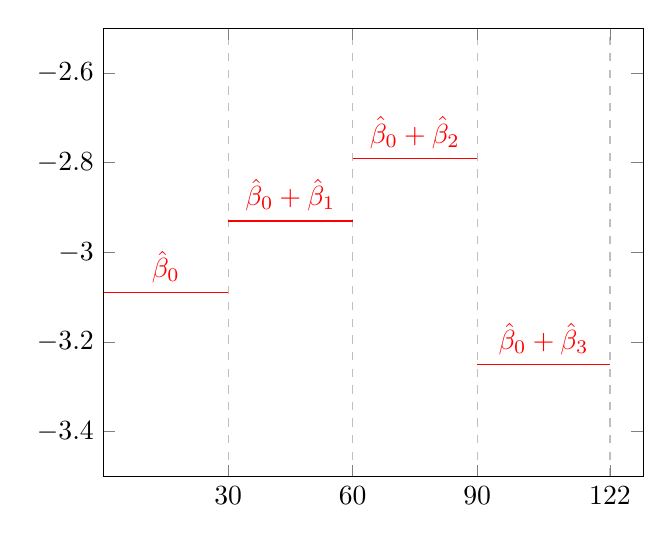
\begin{tikzpicture}
            \begin{axis}[
                        xmin=0, xmax=130,
                        ymin=-3.5, ymax=-2.5,
                        xtick={30,60,90,122},
                        legend pos=north west,
                        ymajorgrids=false,
                        xmajorgrids=true,
                        grid style=dashed,
                  ]
                  \addplot[color=red] coordinates {(0,-3.09)(30,-3.09)} node [anchor=south,midway] (beta){$\hat{\beta}_0$} ;
                  \addplot[color=red] coordinates {(30,-2.93)(60,-2.93)} node [anchor=south,midway] (beta){$\hat{\beta}_0+\hat{\beta}_1$};
                  \addplot[color=red] coordinates {(60,-2.79)(90,-2.79)} node [anchor=south,midway] (beta){$\hat{\beta}_0+\hat{\beta}_2$};
                  \addplot[color=red] coordinates {(90,-3.25)(122,-3.25)} node [anchor=south,midway] (beta){$\hat{\beta}_0+\hat{\beta}_3$};
            \end{axis}
      \end{tikzpicture}
\end{center}
\begin{itemize}
      \item $ \log{\hat{\lambda}_1}=\hat{\beta}_0=-3.09 $.
      \item $ \log{\hat{\lambda}_2}=\hat{\beta}_0+\hat{\beta}_1=-3.09+0.16=-2.93 $.
      \item $ \log{\hat{\lambda}_3}=\hat{\beta}_0+\hat{\beta}_2=-3.09+0.3=-2.79 $.
      \item $ \log{\hat{\lambda}_4}=\hat{\beta}_0+\hat{\beta}_3=-3.09-0.16=-3.25 $.
\end{itemize}
\subsubsection*{Interpretation of \texttt{pfitC}}
\[ \textcolor{Green}{\log{\mu_i}=\beta_0+\underbrace{\beta_1x_{i1}+\beta_2x_{i2}+\beta_3x_{i3}}_{\text{interval}}+\log{t_i}} \]
\begin{itemize}
      \item Relative Rate of events in interval 2 versus interval 1:
            \[ \exp{\beta_1}=\frac{\lambda(\text{interval 2})}{\lambda(\text{interval 1})}=\exp{0.16254}=1.176. \]
      \item Notice none of $ \beta_1,\beta_2,\beta_3 $ are statistically significant.
      \item There is a trend of a slightly higher rate in intervals 2 and 3 (versus interval 1) but
            the event rate does not differ significantly across follow-up time in the control rats.
\end{itemize}
\subsubsection*{2. Model Control and Treatment Groups (\texttt{pfit})}
\begin{itemize}
      \item Now, fit a model to both the treatment and control groups.
      \item $ x_{i4}=\Ind{\text{treatment group}} $.
      \item Assume a piecewise constant baseline rate function.
      \item Model is now:
            \[ \textcolor{Green}{\log{\mu_i}=\beta_0+\underbrace{\beta_1x_{i1}+\beta_2x_{i2}+\beta_3x_{i3}}_{\text{interval}}+\beta_4x_{i4}+\texttt{offset}(\log{t_i})}. \]
      \item $ \exp{\beta_1} $ is now RR of events for interval 2 versus interval 1, for two rats of the
            same treatment group.
\end{itemize}
%\begin{noindent}
\begin{knitrout}
\definecolor{shadecolor}{rgb}{0.969, 0.969, 0.969}\color{fgcolor}\begin{kframe}
\begin{alltt}
\hlstd{pfit} \hlkwb{<-} \hlkwd{glm}\hlstd{(count} \hlopt{~} \hlkwd{factor}\hlstd{(interval)} \hlopt{+} \hlstd{trt} \hlopt{+} \hlkwd{offset}\hlstd{(}\hlkwd{log}\hlstd{(len)),} \hlkwc{family} \hlstd{=} \hlkwd{poisson}\hlstd{(}\hlkwc{link} \hlstd{= log),}
  \hlkwc{data} \hlstd{= rats.pw)}
\hlkwd{summary}\hlstd{(pfit)}
\end{alltt}
\begin{verbatim}

Call:
glm(formula = count ~ factor(interval) + trt + offset(log(len)), 
    family = poisson(link = log), data = rats.pw)

Deviance Residuals: 
    Min       1Q   Median       3Q      Max  
-1.8335  -1.1994  -0.3302   0.4701   3.0551  

Coefficients:
                  Estimate Std. Error z value Pr(>|z|)    
(Intercept)       -3.08818    0.15079 -20.480  < 2e-16 ***
factor(interval)2  0.17185    0.19590   0.877    0.380    
factor(interval)3  0.20634    0.19438   1.062    0.288    
factor(interval)4 -0.06454    0.20412  -0.316    0.752    
trt               -0.82302    0.15171  -5.425 5.79e-08 ***
---
Signif. codes:  0 '***' 0.001 '**' 0.01 '*' 0.05 '.' 0.1 ' ' 1

(Dispersion parameter for poisson family taken to be 1)

    Null deviance: 301.37  on 191  degrees of freedom
Residual deviance: 266.32  on 187  degrees of freedom
AIC: 547.75

Number of Fisher Scoring iterations: 5
\end{verbatim}
\end{kframe}
\end{knitrout}
%\end{noindent}
\subsubsection*{Interpretation of \texttt{pfit}}
\begin{itemize}
      \item Relative Rate of events for treatment versus control rats:
            \[ \exp{\beta_4}=\frac{\lambda(\text{treatment})}{\lambda(\text{control})}=\exp{-0.8230}=0.44. \]
      \item Controlling for interval of follow-up, the rate of tumour development in treated rats
            in $0.44$ times that of control rats.
      \item That is, treatment looks beneficial.
      \item Notice that $ \beta_4 $ is statistically significant.
      \item $ \beta_1,\beta_2,\beta_3 $ are still not statistically significant.
      \item Consider do we really need to use a time non-homogeneous model for this data?
\end{itemize}
\subsubsection*{3. Time Homogeneous Model (\texttt{fit})}
\[ \textcolor{Green}{\log{\mu_i}=\beta_0+\beta_4x_{i4}+\log{t_i}}. \]
\begin{itemize}
      \item $ \beta_0= $ log rate of tumour development, per day, control group.
      \item $ \beta_4= $ log Relative Rate (RR) of tumour development in treated vs control rats.
      \item This model is nested within the time non-homogeneous model.
      \item Consider \texttt{pfit} model with $ \beta_1=\beta_2=\beta_3=0 $.
      \item We can carry out a likelihood ratio test
\end{itemize}
%\begin{noindent}
\begin{knitrout}
\definecolor{shadecolor}{rgb}{0.969, 0.969, 0.969}\color{fgcolor}\begin{kframe}
\begin{alltt}
\hlstd{fit} \hlkwb{<-} \hlkwd{glm}\hlstd{(count} \hlopt{~} \hlstd{trt} \hlopt{+} \hlkwd{offset}\hlstd{(}\hlkwd{log}\hlstd{(len)),} \hlkwc{family} \hlstd{=} \hlkwd{poisson}\hlstd{(}\hlkwc{link} \hlstd{= log),}
  \hlkwc{data} \hlstd{= rats.pw)}
\hlkwd{summary}\hlstd{(fit)}
\end{alltt}
\begin{verbatim}

Call:
glm(formula = count ~ trt + offset(log(len)), family = poisson(link = log), 
    data = rats.pw)

Deviance Residuals: 
    Min       1Q   Median       3Q      Max  
-1.7800  -1.1421  -0.4235   0.4009   3.2673  

Coefficients:
            Estimate Std. Error z value Pr(>|z|)    
(Intercept) -3.00562    0.08138 -36.934  < 2e-16 ***
trt         -0.82302    0.15171  -5.425 5.79e-08 ***
---
Signif. codes:  0 '***' 0.001 '**' 0.01 '*' 0.05 '.' 0.1 ' ' 1

(Dispersion parameter for poisson family taken to be 1)

    Null deviance: 301.37  on 191  degrees of freedom
Residual deviance: 269.06  on 190  degrees of freedom
AIC: 544.49

Number of Fisher Scoring iterations: 5
\end{verbatim}
\end{kframe}
\end{knitrout}
%\end{noindent}
\subsubsection*{Interpretation of \texttt{fit}}
\begin{itemize}
      \item Note $ \hat{\beta}_4=-0.8230 $ is almost unchanged versus model \texttt{fit}.
      \item Likelihood Ratio/Deviance test of $ \HN $: $ \beta_1=\beta_2=\beta_3=0 $:
            \[ \Delta D=D_0-D_A=269.060-266.323 \sim \chi^2_{3}\text{ under $\HN$}. \]
            %\begin{noindent}
\begin{knitrout}
\definecolor{shadecolor}{rgb}{0.969, 0.969, 0.969}\color{fgcolor}\begin{kframe}
\begin{alltt}
\hlnum{1} \hlopt{-} \hlkwd{pchisq}\hlstd{(fit}\hlopt{$}\hlstd{deviance} \hlopt{-} \hlstd{pfit}\hlopt{$}\hlstd{deviance, fit}\hlopt{$}\hlstd{df.residual} \hlopt{-} \hlstd{pfit}\hlopt{$}\hlstd{df.residual)}
\end{alltt}
\begin{verbatim}
[1] 0.4340077
\end{verbatim}
\end{kframe}
\end{knitrout}
    %\end{noindent}
      \item Do not reject $ \HN $.
      \item Conclude that the time homogeneous model (model 3) is probably OK in this case.
      \item However, we retain it for generality and for the following analysis.
\end{itemize}
\subsubsection*{4. Time Non-Homogeneous Model with Treatment Interaction (\texttt{ifit})}
\begin{itemize}
      \item Q: Is the treatment effect constant over time?
      \item Model with interaction:
            \textcolor{Green}{\begin{align*}
                        \log{\mu_i}
                         & =\beta_0+\overbrace{\beta_1x_{i1}+\beta_2x_{i2}+\beta_3x_{i3}}^{\text{interval}}+\overbrace{\beta_4x_{i4}}^{\text{treatment}}+ \\
                         & \quad +\underbrace{\beta_5x_{i1}x_{i4}+\beta_6x_{i2}x_{i4}+\beta_7x_{i3}x_{i4}}_{\text{interval$*$treatment}}+\log{t_i}
                  \end{align*}}
      \item Model \texttt{pfit} (time non-homogeneous, without interaction) is nested within this
            model (consider \texttt{ifit} with $ \beta_5=\beta_6=\beta_7=0 $).
\end{itemize}
%\begin{noindent}
\begin{knitrout}
\definecolor{shadecolor}{rgb}{0.969, 0.969, 0.969}\color{fgcolor}\begin{kframe}
\begin{alltt}
\hlstd{ifit} \hlkwb{<-} \hlkwd{glm}\hlstd{(count} \hlopt{~} \hlkwd{offset}\hlstd{(}\hlkwd{log}\hlstd{(len))} \hlopt{+} \hlkwd{factor}\hlstd{(interval)} \hlopt{*} \hlstd{trt,} \hlkwc{family} \hlstd{=} \hlkwd{poisson}\hlstd{(}\hlkwc{link} \hlstd{= log),}
  \hlkwc{data} \hlstd{= rats.pw)}
\hlkwd{summary}\hlstd{(ifit)}
\end{alltt}
\begin{verbatim}

Call:
glm(formula = count ~ offset(log(len)) + factor(interval) * trt, 
    family = poisson(link = log), data = rats.pw)

Deviance Residuals: 
    Min       1Q   Median       3Q      Max  
-1.9183  -1.2158  -0.3241   0.5125   2.8959  

Coefficients:
                      Estimate Std. Error z value Pr(>|z|)    
(Intercept)           -3.09371    0.17150 -18.039   <2e-16 ***
factor(interval)2      0.16252    0.23326   0.697   0.4860    
factor(interval)3      0.30228    0.22617   1.337   0.1814    
factor(interval)4     -0.15691    0.24833  -0.632   0.5275    
trt                   -0.80392    0.31755  -2.532   0.0114 *  
factor(interval)2:trt  0.03164    0.42972   0.074   0.9413    
factor(interval)3:trt -0.37639    0.44663  -0.843   0.3994    
factor(interval)4:trt  0.28653    0.43808   0.654   0.5131    
---
Signif. codes:  0 '***' 0.001 '**' 0.01 '*' 0.05 '.' 0.1 ' ' 1

(Dispersion parameter for poisson family taken to be 1)

    Null deviance: 301.37  on 191  degrees of freedom
Residual deviance: 263.92  on 184  degrees of freedom
AIC: 551.35

Number of Fisher Scoring iterations: 5
\end{verbatim}
\end{kframe}
\end{knitrout}
%\end{noindent}
\subsubsection*{Interpretation of \texttt{ifit}}
\begin{itemize}
      \item Note $ \hat{\beta}_4=-0.8038 $ is very similar to \texttt{pfit}.
      \item Likelihood Ratio/Deviance test of $ \HN $: $ \beta_5=\beta_6=\beta_7=0 $:
            \[ \Delta D=D_0-D_A=266.323-263.917 \sim \chi^2_{3}\text{ under $\HN$}. \]
            %\begin{noindent}
\begin{knitrout}
\definecolor{shadecolor}{rgb}{0.969, 0.969, 0.969}\color{fgcolor}\begin{kframe}
\begin{alltt}
\hlnum{1} \hlopt{-} \hlkwd{pchisq}\hlstd{(pfit}\hlopt{$}\hlstd{deviance} \hlopt{-} \hlstd{ifit}\hlopt{$}\hlstd{deviance, pfit}\hlopt{$}\hlstd{df.residual} \hlopt{-} \hlstd{ifit}\hlopt{$}\hlstd{df.residual)}
\end{alltt}
\begin{verbatim}
[1] 0.4926145
\end{verbatim}
\end{kframe}
\end{knitrout}
            %\end{noindent}
      \item Do not reject $ \HN $.
      \item We do not have evidence that the treatment effect varies across the time intervals.
\end{itemize}
\subsubsection*{Summary of Rat Tumour Data Analysis}
\begin{itemize}
      \item Looks like a piecewise constant rate function is not necessary.
      \item The best model (of the ones we examined) is \texttt{fit}:
            \[ \textcolor{Green}{\log{\mu_i}=\beta_0+\beta_4x_{i4}+\log{t_i}}. \]
      \item \textcolor{Blue}{Interpretation}: The relative rate for tumour development in treated versus control
            rats is:
            \[ \exp{\hat{\beta}_4}=\exp{-0.822995}=0.439. \]
      \item That is, treatment is beneficial (treated rates get fewer tumours).
      \item \textcolor{Blue}{Prediction}: Expected number of tumours for a treated rat observed for 70 days?
            \[ \log{\hat{\mu}}=\hat{\beta}_0+\hat{\beta}_4+\log{70}=-3.00562-0.82302+\log{70}=0.41986. \]
            \[ \hat{\mu}=\exp{0.41986}=1.5217. \]
\end{itemize}

\section*{Topic 4e: Introduction of Contingency Tables}
\addcontentsline{toc}{section}{Topic 4e: Introduction of Contingency Tables}
\subsection*{Analysis of Contingency Tables}
\addcontentsline{toc}{subsection}{Analysis of Contingency Tables}
\begin{itemize}
    \item Contingency tables can be formed to display data when all variables are categorical.
    \item Below is a two-dimensional $ I\times J $ contingency table.
          \[ \begin{NiceArray}{c|ccccccc|c}[first-row,first-col]
                                                 &        & \Block{1-7}{\text{Factor $ W $}}                                                                                                        \\
                                                 &        & 1                                & 2             & 3             & \cdots & j             & \cdots & J                                  \\
                  \midrule
                  \Block{7-1}{\text{Factor $V$}} & 1      & y_{11}                           & y_{12}        & y_{13}        & \cdots & y_{1j}        & \cdots & y_{1J}        & y_{1\bullet}       \\
                                                 & 2      & y_{21}                           & y_{22}        & y_{23}        & \cdots & y_{2j}        & \cdots & y_{2J}        & y_{2\bullet}       \\
                                                 & 3      & y_{31}                           & y_{32}        & y_{33}        & \cdots & y_{3j}        & \cdots & y_{3J}        & y_{3\bullet}       \\
                                                 & \vdots & \vdots                           & \vdots        & \vdots        & \ddots & \vdots        & \ddots & \vdots        & \vdots             \\
                                                 & i      & y_{i1}                           & y_{i2}        & y_{i3}        & \cdots & y_{ij}        & \cdots & y_{iJ}        & y_{i\bullet}       \\
                                                 & \vdots & \vdots                           & \vdots        & \vdots        & \ddots & \vdots        & \ddots & \vdots        & \vdots             \\
                                                 & I      & y_{I1}                           & y_{I2}        & y_{I3}        & \cdots & y_{Ij}        & \cdots & y_{IJ}        & y_{I\bullet}       \\
                  \midrule
                                                 &        & y_{\bullet 1}                    & y_{\bullet 2} & y_{\bullet 3} & \cdots & y_{\bullet j} & \cdots & y_{\bullet J} & y_{\bullet\bullet}
              \end{NiceArray}. \]
    \item $ I= $ Number of rows; $ J= $ Number of columns.
    \item \textcolor{Blue}{Row Totals}: $ y_{i\bullet}=\sum_{j=1}^{J}y_{ij} $.
    \item \textcolor{Blue}{Column Totals}: $ y_{\bullet j}=\sum_{i=1}^{I}y_{ij} $.
    \item \textcolor{Blue}{Grand Total}: $ y_{\bullet\bullet}=\sum_{i=1}^{I}\sum_{j=1}^{J}y_{ij} $.
    \item Want to assess the nature/significance of ANY associations between the variables.
    \item No special response variable --- all factors are of equal importance.
    \item Contingency tables are a cross-classification of units with respect to the factors of
          interest.
    \item The observations $ y_{ij} $ consist of all the cell counts of the contingency table --- these will be our ``responses.''
\end{itemize}
\subsubsection*{Example: 2-way Contingency Table}
\begin{Example}{Breast Self-Examination Contingency Table}
    \begin{itemize}
        \item Senie \emph{et al}. (1981) investigated the relationship between age and frequency of
              breast self-examination in a sample of women.
        \item Two factors: Age (at 3 levels) and Frequency (at 3 levels).
              \begin{center}
                  \begin{NiceTabular}{c|ccc|c}[first-row,first-col]
                      &&\Block{1-3}{Frequency of breast self-examination}\\
                      && Monthly & Occasionally & Never & Total\\
                      \midrule
                      \Block{3-1}{Age} & $<$45 & $ 91 $ & $ 90 $ & $ 51 $ & $ 232 $\\
                      & 45--59 & $ 150 $ & $ 200 $ & $ 155 $ & $ 505 $\\
                      & $ \ge $60 & $ 109 $ & $ 198 $ & $ 172 $ & $ 479 $\\
                      \midrule
                      & Total & $ 350 $ & $ 488 $ & $ 378 $ & $ 1216 $
                  \end{NiceTabular}
              \end{center}
        \item Is than an association between age and exam frequency?
    \end{itemize}
\end{Example}
\subsubsection*{Basic Assumption in Contingency Tables}
\begin{itemize}
    \item \textcolor{Blue}{Basic Assumption}: Each cell count has an independent Poisson distribution with
          mean $ \mu_{ij} $ for the $ (i,j) $ cell
          \[ \Prob{Y_{ij}=y_{ij}}=\frac{\mu_{ij}^{y_{ij}}e^{-\mu_{ij}}}{y_{ij}!},\;y_{ij}=0,1,2,\ldots. \]
    \item The joint distribution is
          \[ \Prob{Y_{i j}=y_{i j}, i=1, \ldots, I, j=1, \ldots, J}=
              \prod_{i=1}^{I} \prod_{j=1}^{J}\biggl(\frac{\mu_{i j}^{y_{i j}} e^{-\mu_{i j}}}{y_{i j} !}\biggr) \]
    \item We will condition on the relevant fixed totals (row, column, or grand) (possibly
          fixed by design) to get a multinomial or product multinomial distribution.
    \item Will show that these can all by analysed using Poisson GLMs.
\end{itemize}
\subsection*{The Multinomial Distribution}
\addcontentsline{toc}{subsection}{The Multinomial Distribution}
\begin{itemize}
    \item Assume the total number of units is fixed $ Y_{\bullet\bullet}=y_{\bullet\bullet} $ ($ =n $).
    \item Units are then cross-classified by $ 2 $ factors $ V $ and $ W $.
    \item Our assumption of $ Y_{ij}\sim \POI{\mu_{ij}} $ independently implies
          \[ Y_{\bullet\bullet}\sim \POI{\mu_{\bullet\bullet}},\text{ where }\mu_{\bullet\bullet}=\sum\sum \mu_{ij}. \]
    \item To get the joint distribution of the $ Y_{ij} $'s, we must condition on the grand total $ Y_{\bullet\bullet}=y_{\bullet\bullet} $
          since this is a fixed design:
          \begin{align*}
              \Prob{Y_{ij}=y_{ij}\forall i,j\given Y_{\bullet\bullet}=y_{\bullet\bullet}}
               & =\frac{\Prob{Y_{ij}=y_{ij}\forall i,j,Y_{\bullet\bullet}=y_{\bullet\bullet}}}{\Prob{Y_{\bullet\bullet}=y_{\bullet\bullet}}}                                           \\
               & =\frac{\prod_{i=1}^{I} \prod_{j=1}^{J}\biggl(\frac{\mu_{i j}^{y_{i j}} \exp{-\mu_{i j}}}{y_{i j} !}\biggr)}{
              \mu_{\bullet\bullet}^{y_{\bullet\bullet}}\exp{-\mu_{\bullet\bullet}}/y_{\bullet\bullet}!
              }                                                                                                                                                                        \\
               & =\biggl(\frac{y_{\bullet\bullet}!}{\prod\prod y_{ij}!}\biggr)\biggl(\frac{\prod\prod \mu_{ij}^{y_{ij}}}{\mu_{\bullet\bullet}^{y_{\bullet\bullet}}}\biggr)
              \underbrace{\biggl(\frac{\exp*{-\sum\sum \mu_{ij}}}{\exp{-\mu_{\bullet\bullet}}}\biggr)}_{\textcolor{Green}{\text{$=1$ since $\mu_{\bullet\bullet}=\sum\sum \mu_{ij}$}}} \\
               & =\biggl(\frac{y_{\bullet\bullet}!}{\prod\prod y_{ij}!}\biggr)
              \underbrace{\prod_{i=1}^I \prod_{j=1}^J \biggl(\frac{\mu_{ij}}{\mu_{\bullet\bullet}}\biggr)^{\! y_{ij}}}_{\textcolor{Green}{\text{since $\mu_{\bullet\bullet}^{y_{\bullet\bullet}}=\mu_{\bullet\bullet}^{\sum\sum y_{ij}}=\prod\prod \mu_{\bullet\bullet}^{y_{ij}}$}}}
          \end{align*}
    \item Recall the standard \textcolor{Blue}{Multinomial distribution}:
          \[ f(x_1,\ldots,x_k;n,\pi_1,\ldots,\pi_k)=\Prob{X_1=x_1,\ldots,X_k=x_k}=\frac{n!}{x_1!\cdots x_k!}\pi_1^{x_1}\cdots \pi_k^{x_k}, \]
          where $ \sum \pi_i=1 $ and $ \sum x_i=n $.
    \item The pmf on the previous slide is a multinomial distribution with
          \[ \pi_{ij}=\mu_{ij}/\mu_{\bullet\bullet}=\Prob{\text{level $i$ of factor $V$ and level $j$ of factor $W$}}. \]
    \item Note that $\sum\sum \pi_{ij}=1$
          \[ \textcolor{Blue}{\Prob{Y_{ij}=y_{ij}\forall i,j\given Y_{\bullet\bullet}=y_{\bullet\bullet}}
              =\biggl(\frac{y_{\bullet\bullet}!}{\prod\prod y_{ij}!}\biggr)\prod_{i=1}^I \prod_{j=1}^J \pi_{ij}^{y_{ij}}}. \]
\end{itemize}
\subsubsection*{Multinomial Likelihood}
\[ \Prob{Y_{ij}=y_{ij}\forall i,j\given Y_{\bullet\bullet}=y_{\bullet\bullet}}
    =\biggl(\frac{y_{\bullet\bullet}!}{\prod\prod y_{ij}!}\biggr)\prod_{i=1}^I \prod_{j=1}^J \pi_{ij}^{y_{ij}}. \]
\begin{itemize}
    \item $ \Vector{\pi}=(\pi_{11},\ldots,\pi_{IJ})^\top $ be the parameter vector.
    \item The likelihood and log-likelihood are given by:
          \[ L(\Vector{\pi})=\prod_i\prod_j \pi_{ij}^{y_{ij}},\text{ where }\sum\sum \pi_{ij}=1 \]
          \[ \ell(\Vector{\pi})=\sum_i\sum_j y_{ij}\log{\pi_{ij}}. \]
\end{itemize}
\subsubsection*{Testing for Independence in a 2-way Table}
\begin{itemize}
    \item Thinking back to the contingency table, we might be interested in testing the
          hypothesis that the two methods of classification are \textcolor{Blue}{independent}:
          \[ \HN\colon \pi_{ij}=\pi_{i\bullet}\pi_{\bullet j}\;\forall i,j \]
          \[ \HA\colon \pi_{ij}\ne \pi_{i\bullet}\pi_{\bullet j}\;\text{for some } i,j, \]
          where $ \pi_{i\bullet}=\sum_{j=1}^{J}\pi_{ij} $ and $ \pi_{\bullet j}=\sum_{i=1}^{I}\pi_{ij} $.
    \item Consider the log-likelihood \textcolor{Blue}{under $ \HN $ (independence)}:
          \begin{align*}
              \ell(\Vector{\pi})
               & =\sum_{i} \sum_{j} y_{i j} \log{\pi_{i\bullet} \pi_{\bullet j}}                             \\
               & =\sum_{i} \sum_{j} y_{i j}\bigl(\log{\pi_{i\bullet}} +\log{\pi_{\bullet j}} \bigr)          \\
               & =\sum_{i} y_{i \bullet} \log{\pi_{i \bullet}}+\sum_{j} y_{\bullet j} \log{\pi_{\bullet j}}.
          \end{align*}
    \item The parameters are constrained by $ \sum \pi_{i\bullet}=1 $ and $ \sum \pi_{\bullet j}=1 $.
    \item The MLEs of $ \pi_{i\bullet} $ and $ \pi_{\bullet j}  $ under $ \HN $ are:
          \[ \hat{\pi}_{i\bullet}=\frac{y_{i\bullet}}{y_{\bullet\bullet}},\qquad \hat{\pi}_{\bullet j}=\frac{y_{\bullet j}}{y_{\bullet\bullet}}. \]
    \item And the log-likelihood evaluated at the MLE is:
          \[ \ell(\hat{\Vector{\pi}})=\sum_{i} \sum_{j} y_{i j} \log*{\frac{y_{i \bullet} y_{\bullet j}}{y_{\bullet\bullet}^{2}}}. \]
    \item Next consider working \textcolor{Blue}{under $ \HA $ (unconstrained)}.
    \item The unconstrained MLEs are: $ \tilde{\pi}_{ij}=\frac{y_{ij}}{y_{\bullet\bullet}} $.
    \item And the log-likelihood evaluated at the unconstrained MLE is:
          \[ \ell(\tilde{\Vector{\pi}})=\sum_{i} \sum_{j} y_{i j} \log*{\frac{y_{ij}}{y_{\bullet\bullet}}}. \]
    \item To test for independence we could use a \textcolor{Blue}{Likelihood Ratio/Deviance} test for the
          multinomial:
          \begin{align*}
              D
               & =2\bigl(\ell(\tilde{\Vector{\pi}})-\ell(\hat{\Vector{\pi}})\bigr)                                                             \\
               & =2\sum_i\sum_j y_{ij}\log*{\frac{y_{ij}}{y_{\bullet\bullet}}\bigg/\frac{y_{i \bullet} y_{\bullet j}}{y_{\bullet\bullet}^{2}}} \\
               & =2\sum_i\sum_j y_{ij}\log*{\frac{y_{ij}}{y_{i\bullet}y_{\bullet j}/y_{\bullet\bullet}}}                                       \\
               & =2\sum_i\sum_j O_{ij}\log*{\frac{O_{ij}}{E_{ij}}}.
          \end{align*}
    \item Note this has the usual form of a Deviance Statistic with
          \[ O_{ij}=y_{ij}\quad\text{ and }\quad E_{ij}=y_{\bullet\bullet}\hat{\pi}_{ij}\text{ under $ \HN $}. \]
    \item We know $ D \sim \chi^2_{n-p)} $, but what are the degrees of freedom here?
          \begin{align*}
              n-p
               & =(\text{\# parameters saturated})-(\text{\# parameters unsaturated}) \\
               & =(IJ-1)-\bigl((I-1)+(J-1)\bigr)                                      \\
               & =IJ-I-J+1                                                            \\
               & =(I-1)(J-1).
          \end{align*}
\end{itemize}
\subsubsection*{Example: Breast Self-Examination Data ($ \tilde{\mu}_{ij} $ vs $ \hat{\mu}_{ij} $)}
\begin{itemize}
    \item \textcolor{Blue}{Observed Data}: $ y_{ij}=\tilde{\mu}_{ij}=\tilde{\pi}_{ij}y_{\bullet\bullet} $:
          \begin{table}[H]
              \centering
              \begin{NiceTabular}{c|ccc|c}[first-row,first-col]
                  &           & \Block{1-3}{Frequency of breast self-examination}                                     \\
                  &           & Monthly                                           & Occasionally & Never   & Total    \\
                  \midrule
                  \Block{3-1}{Age} & $<$45     & $ 91 $                                            & $ 90 $       & $ 51 $  & $ 232 $  \\
                  & 45--59    & $ 150 $                                           & $ 200 $      & $ 155 $ & $ 505 $  \\
                  & $ \ge $60 & $ 109 $                                           & $ 198 $      & $ 172 $ & $ 479 $  \\
                  \midrule
                  & Total     & $ 350 $                                           & $ 488 $      & $ 378 $ & $ 1216 $
              \end{NiceTabular}
          \end{table}
    \item \textcolor{Blue}{Expected Data under $ \HN $}: $ \hat{\mu}_{ij}=\hat{\pi}_{ij}y_{\bullet\bullet}=y_{i\bullet}y_{\bullet j}/y_{\bullet\bullet} $:
          \begin{table}[H]
              \centering
              \begin{NiceTabular}{c|ccc|c}[first-row,first-col]
                  &           & \Block{1-3}{Frequency of breast self-examination}                                        \\
                  &           & Monthly                                           & Occasionally & Never      & Total    \\
                  \midrule
                  \Block{3-1}{Age} & $<$45     & $ 66.78 $                                         & $ 93.11 $    & $ 72.12 $  & $ 232 $  \\
                  & 45--59    & $ 145.35 $                                        & $ 202.66 $   & $ 156.98 $ & $ 505 $  \\
                  & $ \ge $60 & $ 137.87 $                                        & $ 192.23 $   & $ 148.90 $ & $ 479 $  \\
                  \midrule
                  & Total     & $ 350 $                                           & $ 488 $      & $ 378 $    & $ 1216 $
              \end{NiceTabular}
          \end{table}
\end{itemize}
\subsubsection*{Example: Breast Self-Examination Data: ($ \tilde{\pi}_{ij} $ vs $ \hat{\pi}_{ij} $)}
\begin{itemize}
    \item \textcolor{Blue}{Unconstrained MLEs}: $ \tilde{\pi}_{ij}=y_{ij}/y_{\bullet\bullet} $ (as percentages):
          \begin{table}[H]
              \centering
              \begin{NiceTabular}{c|ccc|c}[first-row,first-col]
                  &           & \Block{1-3}{Frequency of breast self-examination}                                        \\
                  &           & Monthly                                           & Occasionally & Never      & Row \%    \\
                  \midrule
                  \Block{3-1}{Age} & $<$45     & $ 7.48 $                         & $ 7.40 $    & $ 4.19 $  & $ 19.07 $  \\
                  & 45--59                     & $ 12.34 $                       & $ 16.45 $   & $ 12.75 $ & $ 41.54 $  \\
                  & $ \ge $60                  & $ 8.96 $                       & $ 16.28 $   & $ 14.14 $ & $ 39.38 $  \\
                  \midrule
                  & Column \%                       & $ 28.78 $                         & $ 40.13 $      & $ 31.08 $    & $ 100 $
              \end{NiceTabular}
          \end{table}
    \item \textcolor{Blue}{Constrained MLEs under $ \HN $}: $ \hat{\pi}_{ij}=\hat{\pi}_{i\bullet}\hat{\pi}_{\bullet j}=y_{i\bullet}y_{\bullet j}/y_{\bullet\bullet}^2 $:
          \begin{table}[H]
              \centering
              \begin{NiceTabular}{c|ccc|c}[first-row,first-col]
                  &           & \Block{1-3}{Frequency of breast self-examination}                                        \\
                  &           & Monthly                                           & Occasionally & Never      & Row \%    \\
                  \midrule
                  \Block{3-1}{Age} & $<$45     & $ 5.49 $                         & $ 7.66 $    & $ 5.93 $  & $ 19.08 $  \\
                  & 45--59                     & $ 11.95 $                       & $ 16.67 $   & $ 12.91 $ & $ 41.53 $  \\
                  & $ \ge $60                  & $ 11.34 $                       & $ 15.81 $   & $ 12.25 $ & $ 39.40 $  \\
                  \midrule
                  & Column \%                       & $ 28.78 $                         & $ 40.14  $      & $ 31.09 $    & $ 100 $
              \end{NiceTabular}
          \end{table}
\end{itemize}
\subsubsection*{Example: Breast Self-Examination Data (Testing Independence)}
\begin{itemize}
    \item Use the Likelihood Ratio/Deviance test derived for the Multinomial Distribution
          \[ D=2\sum_i\sum_j y_{ij}\log*{\frac{y_{ij}}{y_{i\bullet}y_{\bullet j}/y_{\bullet\bullet}}}=25.19226. \]
    \item Compare to a $ \chi^2_{4} $ distribution:
          \[ p=\Prob*{\chi^2_{4}>25.19226}<0.001. \]
    \item So we reject the null hypothesis that age and frequency of breast self-examination
          are independent.
\end{itemize}
\subsection*{The Product Multinomial Distribution}
\addcontentsline{toc}{subsection}{The Product Multinomial Distribution}
\begin{itemize}
    \item Previously, we assumed the grand total $ Y_{\bullet\bullet}=y_{\bullet\bullet} $ was fixed.
    \item Now assume that the \textcolor{Blue}{row totals} $ Y_{i\bullet}=y_{i\bullet} $ are fixed.
          \begin{itemize}
              \item Choose a sample of fixed size from populations $ i=1,\ldots,I $ and then classify the
                    units with response to Factor $W$.
          \end{itemize}
    \item Our assumption of $ Y_{ij}\sim \POI{\mu_{ij}} $ independently implies
          \[ Y_{i\bullet}\sim \POI{\mu_{i\bullet}},\text{ where }\mu_{i\bullet}=\sum_{j}\mu_{ij}. \]
    \item To get the joint distribution of the $ Y_{ij} $'s we now condition on the row totals
          $ Y_{i\bullet}=y_{i\bullet} $, $ i=1,\ldots,I $
          \[ \Prob{Y_{ij}=y_{ij}\forall i,j\given Y_{i\bullet}=y_{i\bullet}\forall i}
              =\frac{\Prob{Y_{ij}=y_{ij}\forall i,j,Y_{i\bullet}=y_{i\bullet}\forall i}}{\Prob{Y_{i\bullet}=y_{i\bullet}\forall i}}.     \]
\end{itemize}
\subsubsection*{Example: Another Breast Self-Examination Study}
\begin{itemize}
    \item Imagine this time the investigators decided study a fixed number of women of
          each age group.
    \item The (hypothetical) 2-way contingency table is now:
          \begin{Example}{Breast Self-Examination Contingency Table (Hypothetical)}
              \begin{center}
                  \begin{NiceTabular}{c|ccc|c}[first-row,first-col]
                      &&\Block{1-3}{Frequency of breast self-examination}\\
                      && Monthly & Occasionally & Never & Total\\
                      \midrule
                      \Block{3-1}{Age} & $<$45 & $ 78 $ & $ 78 $ & $ 44 $ & $ 200 $\\
                      & 45--59 & $ 178 $ & $ 238 $ & $ 184 $ & $ 600 $\\
                      & $ \ge $60 & $ 91 $ & $ 165 $ & $ 144 $ & $ 400 $\\
                      \midrule
                      & Total & $ 347 $ & $ 481 $ & $ 372 $ & $ 1200 $
                  \end{NiceTabular}
              \end{center}
          \end{Example}
    \item We need to take this method of sampling into account in the analysis.
\end{itemize}
\begin{align*}
    \Prob{Y_{ij}=y_{ij}\forall i,j\given Y_{i\bullet}=y_{i\bullet}\forall i}
     & =\biggl(\prod_i \prod_j \biggl(\frac{\mu_{ij}^{y_{ij}} \exp{-\mu_{ij}}}{y_{ij}!}\biggr)\biggr)\Bigg/\biggl(\prod_i \frac{\mu_{i\bullet}^{y_{i\bullet}}\exp{-\mu_{i\bullet}}}{y_{i\bullet}!}\biggr)             \\
     & =\biggl(\frac{\prod_i y_{i\bullet}!}{\prod\prod y_{ij}!}\biggr)\biggl(\frac{\prod\prod \mu_{ij}^{y_{ij}}}{\prod_i \mu_{i\bullet}^{y_{i\bullet}}}\biggr)
    \underbrace{\biggl(\frac{\exp{-\sum\sum \mu_{ij}}}{\exp{-\sum_i \mu_i}}\biggr)}_{\textcolor{Green}{\text{$=1$ since $\mu_{i j}=\sum_i \mu_{i\bullet}=\mu_{\bullet\bullet}$ }}}                                    \\
     & =\prod_{i=1}^I \underbrace{\biggl(\frac{y_{i\bullet}!}{\prod_j y_{ij}!}\prod_{j=1}^J \biggl(\frac{\mu_{ij}}{\mu_{i\bullet}}\biggr)^{\!y_{ij}}\biggr)}_{\textcolor{Green}{\text{Multinomial pmf for row $i$}}}.
\end{align*}
\begin{itemize}
    \item This is the \textcolor{Blue}{product multinomial distribution} with $ \pi_{ij}=\mu_{ij}/\mu_{i\bullet} $.
    \item Here, $ \pi_{ij}= $ probability of being level $j$ given population level $i$.
    \item Note that $ \sum_j \pi_{ij}=1 $ for all $ i $.
\end{itemize}
\subsubsection*{Product Multinomial Likelihood}
\[ \Prob{Y_{ij}=y_{ij}\forall i,j\given Y_{i\bullet}=y_{i\bullet}\forall i}=
    \prod_{i=1}^I\biggl(\frac{y_{i\bullet}!}{\prod_j y_{ij}!}\prod_{j=1}^J \pi_{ij}^{y_{ij}}\biggr). \]
\begin{itemize}
    \item Again, let $ \Vector{\pi}=(\pi_{11},\ldots,\pi_{IJ})^\top $ be the parameter vector.
    \item Note the $ \pi_{ij} $ have different interpretations here versus the multinomial case.
    \item The log-likelihood is given by:
          \[ \ell(\Vector{\pi})=\sum_i\sum_j y_{ij}\log{\pi_{ij}},\text{ where }\sum_j \pi_{ij}=1\;\forall i. \]
\end{itemize}
\subsubsection*{Testing for Independence with the Product Multinomial}
\begin{itemize}
    \item In this case we might be interested in testing where the probability of being at
          factor level $j$ is the same across all stratum/populations $ i=1,\ldots,I $
          \[ \HN\colon \pi_{1j}=\pi_{2j}=\cdots=\pi_{Ij}=\pi_j,\;j=1,2,\ldots,J, \]
          \[ \HA\colon \text{at least one }\pi_{ij}\ne \pi_{i^\prime j}. \]
    \item The log likelihood \textcolor{Blue}{under $ \HN $ (independence)} is
          \[ \ell(\Vector{\pi})=\sum_i\sum_j y_{ij}\log{\pi_{j}}=\sum_j y_{\bullet j}\log{\pi_{j}}. \]
    \item The parameters are constrained by $ \sum_{j}\pi_j=1 $.
    \item The MLEs under $ \HN $ are
          \[ \hat{\pi}_{ij}=\hat{\pi}_j=\frac{y_{\bullet j}}{y_{\bullet\bullet}}. \]
    \item \textcolor{Blue}{Under $ \HA $ (unconstrained)} the MLEs are
          \[ \tilde{\pi}_{ij}=\frac{y_{ij}}{y_{i\bullet}}. \]
    \item The \textcolor{Blue}{Likelihood Ratio/Deviance} test statistic is:
          \begin{align*}
              D
               & =2\bigl(\ell(\tilde{\Vector{\pi}})-\ell(\hat{\Vector{\pi}})\bigr)                                     \\
               & =2\sum_i\sum_j y_{ij}\log*{\frac{y_{ij}}{y_{i\bullet}}\bigg/\frac{y_{\bullet j}}{y_{\bullet\bullet}}} \\
               & =2\sum_i\sum_j y_{ij}\log*{\frac{y_{ij}}{y_{i\bullet}y_{\bullet j}/y_{\bullet\bullet}}}.
          \end{align*}
    \item Which is identical to the Deviance statistic for testing independence under a
          multinomial distribution.
    \item Here, $ D \sim \chi^2_{(I-1)(J-1)} $ since
          \[ n-p=I(J-1)-(J-1)=IJ-I-J+1=(I-1)(J-1). \]
\end{itemize}
\subsubsection*{Example: Another Breast Self-Examination Study}
\begin{itemize}
    \item \textcolor{Blue}{Observed Data}: $ y_{ij} $:
          \begin{table}[H]
              \centering
              \begin{NiceTabular}{c|ccc|c}[first-row,first-col]
                  &&\Block{1-3}{Frequency of breast self-examination}\\
                  && Monthly & Occasionally & Never & Total\\
                  \midrule
                  \Block{3-1}{Age} & $<$45 & $ 78 $ & $ 78 $ & $ 44 $ & $ 200 $\\
                  & 45--59 & $ 178 $ & $ 238 $ & $ 184 $ & $ 600 $\\
                  & $ \ge $60 & $ 91 $ & $ 165 $ & $ 144 $ & $ 400 $\\
                  \midrule
                  & Total & $ 347 $ & $ 481 $ & $ 372 $ & $ 1200 $
              \end{NiceTabular}
          \end{table}
    \item \textcolor{Blue}{Expected Data under $ \HN $}: $ \hat{\mu}_{ij}=y_{i\bullet}\hat{\pi}_j=y_{i\bullet}y_{\bullet j}/y_{\bullet\bullet} $
          \begin{table}[H]
              \centering
              \begin{NiceTabular}{c|ccc|c}[first-row,first-col]
                  &&\Block{1-3}{Frequency of breast self-examination}\\
                  && Monthly & Occasionally & Never & Total\\
                  \midrule
                  \Block{3-1}{Age} & $<$45 & $ 57.83 $ & $ 80.17 $ & $ 62.00 $ & $ 200 $\\
                  & 45--59 & $ 173.50 $ & $ 240.50 $ & $ 186.00 $ & $ 600 $\\
                  & $ \ge $60 & $ 115.67 $ & $ 160.33 $ & $ 124.00 $ & $ 400 $\\
                  \midrule
                  & Total & $ 347 $ & $ 481 $ & $ 372 $ & $ 1200 $
              \end{NiceTabular}
          \end{table}
    \item \textcolor{Blue}{Unconstrained MLEs}: $ \tilde{\pi}_{ij}=y_{ij}/y_{i\bullet} $ (as percentages):
          \begin{table}[H]
              \centering
              \begin{NiceTabular}{c|ccc|c}[first-row,first-col]
                  &&\Block{1-3}{Frequency of breast self-examination}\\
                  && Monthly & Occasionally & Never & Total\\
                  \midrule
                  \Block{3-1}{Age} & $<$45 & $ 39.00 $ & $ 39.00 $ & $ 22.00 $ & $ 100 $\\
                  & 45--59 & $ 29.67 $ & $ 39.67 $ & $ 30.67 $ & $ 100 $\\
                  & $ \ge $60 & $ 22.75 $ & $ 41.25 $ & $ 36.00 $ & $ 100 $\\
                  \bottomrule
              \end{NiceTabular}
          \end{table}
    \item \textcolor{Blue}{Constrained MLEs}: $ \hat{\pi}_{ij}=\hat{\pi}_j=y_{\bullet j}/y_{\bullet\bullet} $ (as percentages):
          \begin{table}[H]
              \centering
              \begin{NiceTabular}{c|ccc|c}[first-row,first-col]
                  &&\Block{1-3}{Frequency of breast self-examination}\\
                  && Monthly & Occasionally & Never & Total\\
                  \midrule
                  \Block{3-1}{Age} & $<$45 & $ 28.92 $ & $ 40.08 $ & $ 31.00 $ & $ 100 $\\
                  & 45--59 & $ 28.92 $ & $ 40.08 $ & $ 31.00 $ & $ 100 $\\
                  & $ \ge $60 & $ 28.92 $ & $ 40.08 $ & $ 31.00 $ & $ 100 $\\
                  \bottomrule
              \end{NiceTabular}
          \end{table}
\end{itemize}
\subsubsection*{Example: Another Breast Self-Examination Study (Testing Independence)}
\begin{itemize}
    \item Use the Likelihood Ratio/Deviance test derived for the Multinomial Distribution
          \[ D=2\sum_i\sum_j y_{ij}\log*{\frac{y_{ij}}{y_{i\bullet}y_{\bullet j}/y_{\bullet\bullet}}}=21.25615. \]
    \item Compare to a $ \chi^2_{4} $ distribution:
          \[ p=\Prob*{\chi^2_{4}>21.25615}<0.001. \]
    \item So we reject the null hypothesis that age and frequency of breast self-examination
          are independent.
\end{itemize}
\subsubsection*{Summary}
\begin{itemize}
    \item Today we considered simple 2-way contingency tables.
    \item With the basic Poisson assumption for the cell counts, depending on the type of
          sampling used, we can test for independence using:
          \begin{enumerate}[1.]
              \item Multinomial distribution (condition on $ y_{\bullet\bullet} $).
              \item Product multinomial (condition on $ y_{i\bullet} $, $ i=1,2,\ldots,I $).
          \end{enumerate}
    \item Both yield the same Likelihood Ratio/Deviance test statistic.
    \item Interestingly we can also use log-linear models to assess these independence
          hypotheses (next week).
    \item Easily generalizable to 3-way (and more) contingency tables.
\end{itemize}
% Week 10

\makeheading{Week 10}{\daterange{2021-11-08}{2021-11-12}}
\section*{Topic 4f: Log Linear Models for Two-way Tables}
\addcontentsline{toc}{section}{Topic 4f: Log Linear Models for Two-way Tables}
\subsubsection*{Likelihood Based Analysis of 2-way Contingency Tables}
\[ \begin{NiceArray}{c|ccccccc|c}[first-row,first-col]
                                       &        & \Block{1-7}{\text{Factor $ W $}}                                                                                                        \\
                                       &        & 1                                & 2             & 3             & \cdots & j             & \cdots & J                                  \\
        \midrule
        \Block{7-1}{\text{Factor $V$}} & 1      & y_{11}                           & y_{12}        & y_{13}        & \cdots & y_{1j}        & \cdots & y_{1J}        & y_{1\bullet}       \\
                                       & 2      & y_{21}                           & y_{22}        & y_{23}        & \cdots & y_{2j}        & \cdots & y_{2J}        & y_{2\bullet}       \\
                                       & 3      & y_{31}                           & y_{32}        & y_{33}        & \cdots & y_{3j}        & \cdots & y_{3J}        & y_{3\bullet}       \\
                                       & \vdots & \vdots                           & \vdots        & \vdots        & \ddots & \vdots        & \ddots & \vdots        & \vdots             \\
                                       & i      & y_{i1}                           & y_{i2}        & y_{i3}        & \cdots & y_{ij}        & \cdots & y_{iJ}        & y_{i\bullet}       \\
                                       & \vdots & \vdots                           & \vdots        & \vdots        & \ddots & \vdots        & \ddots & \vdots        & \vdots             \\
                                       & I      & y_{I1}                           & y_{I2}        & y_{I3}        & \cdots & y_{Ij}        & \cdots & y_{IJ}        & y_{I\bullet}       \\
        \midrule
                                       &        & y_{\bullet 1}                    & y_{\bullet 2} & y_{\bullet 3} & \cdots & y_{\bullet j} & \cdots & y_{\bullet J} & y_{\bullet\bullet}
    \end{NiceArray}. \]
\begin{itemize}
    \item Previously: Previously: Derived Likelihood Ratio/Deviance tests for testing for \textcolor{Blue}{independence}
          between Factor $V$ and Factor $W$.
    \item \textcolor{Blue}{Basic Assumption}: $ Y_{ij} \sim \POI{\mu_{ij}} $, $ \forall i,j $.
    \item When we condition on the Grand Total the joint distribution becomes Multinomial,
          and we want to test:
          \[ \HN\colon \pi_{ij}=\pi_{i\bullet}\pi_{\bullet j}\;\forall i,j \]
          \[ \HA\colon \pi_{ij}\ne \pi_{i\bullet}\pi_{\bullet j}\;\text{for some } i,j. \]
    \item When we condition on the Row Totals the joint distribution becomes \textcolor{Blue}{Product
              Multinomial}, and we want to test:
          \[ \HN\colon \pi_{1j}=\pi_{2j}=\cdots=\pi_{Ij}=\pi_j,\;j=1,2,\ldots,J, \]
          \[ \HA\colon \text{at least one }\pi_{ij}\ne \pi_{i^\prime j}. \]
    \item In either case, the \textcolor{Blue}{Likelihood Ratio/Deviance Test} statistic is:
          \[ D=2\sum_i\sum_j y_{ij}\log*{\frac{y_{ij}}{y_{i\bullet}y_{\bullet j}/y_{\bullet\bullet}}} \sim \chi^2_{(I-1)(J-1)}\text{ under $ \HN $}.\]
\end{itemize}
\subsection*{Log Linear Models for 2-way Contingency Tables}
\addcontentsline{toc}{subsection}{Log Linear Models for 2-way Tables}
\begin{itemize}
    \item \textcolor{Blue}{Basic Assumption}: $ Y_{ij} \sim \POI{\mu_{ij}} $, $ \forall i,j $.
    \item \textcolor{Blue}{Explanatory Variables}: Factor $V$ and $W$:
          \[ \begin{array}{cc}
                  \begin{aligned}
                      x_1     & =\Ind{\text{Factor $V$ at level 2}}, \\
                      x_2     & =\Ind{\text{Factor $V$ at level 3}}, \\
                              & \vdotswithin{=}                      \\
                      x_{I-1} & =\Ind{\text{Factor $V$ at level I}}, \\
                  \end{aligned} &
                  \begin{aligned}
                      x_I       & =\Ind{\text{Factor $W$ at level 2}}, \\
                      x_{I+1}   & =\Ind{\text{Factor $W$ at level 3}}, \\
                                & \vdotswithin{=}                      \\
                      x_{I+J-2} & =\Ind{\text{Factor $W$ at level J}}. \\
                  \end{aligned}
              \end{array} \]
    \item The main effects log-linear model would be:
          \begin{align*}
              \log{\mu_\ell}
               & =\beta_0+\overbrace{\beta_1x_{1\ell}+\beta_2x_{2\ell}+\cdots+\beta_{I-1}x_{I-1\ell}}^{\text{Factor $V$}}+                               \\
               & \quad+\underbrace{\beta_Ix_{I\ell}+\beta_{I+1}x_{I+1\ell}+\cdots+\beta_{I+J-2}x_{I+J-2\ell}}_{\text{Factor $W$}} &  & \ell=1,\ldots,IJ.
          \end{align*}
    \item Note: $ \text{\# parameters}=1+(I-1)+(J-1)=I+J-1 $.
    \item The $ \Vector{x}^\top \Vector{\beta} $ is quite cumbersome when $ I $ and $ J $ are large.
    \item Consider the following expression for the model:
          \[ \log{\mu_{ij}}=u+u_i^V+u_j^W,\;i=1,\ldots,I,\,j=1,\ldots,J, \]
          where $ u_1^V+u_1^W=0 $.
    \item Note: $ \text{\# parameters}=1+(I-1)+(J-1)=I+J-1 $.
    \item This notation suppresses the binary $ x $ variables.
    \item The relationship between the $ \beta $ and $ u $ is as follows:
          \[ \begin{array}{ccc}
                  u=\beta_0,                 &
                  \begin{aligned}
                      u_2^V & =\beta_1,       \\
                      u_3^V & =\beta_2,       \\
                            & \vdotswithin{=} \\
                      u_I^V & =\beta_{I-1},
                  \end{aligned} &
                  \begin{aligned}
                      u_2^W & =\beta_I,       \\
                      u_3^W & =\beta_{I+1},   \\
                            & \vdotswithin{=} \\
                      u_J^W & =\beta_{I+J-2}.
                  \end{aligned}
              \end{array} \]
    \item Testing independence in a 2-way table:
          \[ \HN\colon \pi_{ij}=\pi_{i\bullet}\pi_{\bullet j}\;\forall i,j \]
          \[ \HA\colon \pi_{ij}\ne \pi_{i\bullet}\pi_{\bullet j}\;\text{for some } i,j. \]
    \item The corresponding log-linear models are:
          \[ \HN\colon \log{\mu_{ij}}=u+u_i^V+u_j^W \]
          \[ \HA\colon\log{\mu_{ij}}=u+u_i^V+u_j^W+u_{ij}^{VW}. \]
    \item Using \textcolor{Blue}{corner-point constraints} we require:
          \[ u_1^V=0,\qquad u_1^W=0,\qquad u_{1j}^{VW}=0\;\forall j,\qquad u_{i1}^{VW}\;\forall i. \]
    \item The interaction model has $ 1+(I-1)+(J-1)+(I-1)(J-1)=IJ $ parameters.
    \item \textcolor{Red}{Wait}: We're using a \textcolor{Blue}{Poisson} model to fit data/test hypotheses from a \textcolor{Blue}{Multinomial} distribution?
    \item Examine the log-likelihood from the Poisson:
          \[ \ell(\Vector{\mu})=\sum_i\sum_j\bigl[y_{ij}\log{\mu_{ij}}-\mu_{ij}-\log{y_{ij}!}\bigr]. \]
    \item Substitute in the log linear model \textcolor{Blue}{$ \HN\colon \log{\mu_{ij}}=u+u_i^V+u_j^W $}:
          \begin{align*}
              \ell(\Vector{u})
                            & =\sum\sum\bigl(y_{ij}(\textcolor{Blue}{u+u_i^V+u_j^W})-\exp{\textcolor{Blue}{u+u_i^V+u_j^W}}-\log{y_{ij}!}\bigr)          \\
              \pdv{\ell}{u} & =\sum\sum\bigl(y_{ij}-\exp{u+u_i^V+u_j^W}\bigr)                                                                           \\
                            & =\sum\sum(y_{ij}-\mu_{ij})                                                                                                \\
                            & =y_{\bullet\bullet}-\mu_{\bullet\bullet}\qquad \text{(set $=0$)}\implies \hat{\mu}_{\bullet\bullet}=y_{\bullet\bullet}.   \\
              \pdv{\ell}{u_{i^\star}^V}
                            & =\sum\sum\bigl(y_{i^\star j}-\exp{u+u_{i^\star}^V+u_j^W}\bigr)                                                            \\
                            & =y_{i^\star\bullet}-\mu_{i^\star\bullet}\qquad \text{(set $=0$)}\implies\hat{\mu}_{i\bullet}=y_{i\bullet}\;\forall i.     \\
              \pdv{\ell}{u_{j^\star}^W}
                            & =\sum\sum\bigl(y_{ij^\star}-\exp{u+u_{i}^V+u_{j^\star}^W}\bigr)                                                           \\
                            & =y_{\bullet j^\star}-\mu_{\bullet j^\star}\qquad \text{(set $=0$)}\implies\hat{\mu}_{\bullet j}=y_{\bullet j}\;\forall j.
          \end{align*}
    \item So the main effects log linear model reproduces the row, column and grand totals.
    \item If we do the same with the saturated model
          \[ \HA\colon\log{\mu_{ij}}=u+u_i^V+u_j^W+u_{ij}^{VW}, \]
          we find it provides a perfect fit to the data: $ \tilde{\mu}_{ij}=y_{ij} $ for all $ i,j $.
    \item Recall the Deviance Test for the Poisson Distribution
          \begin{align*}
              D
               & =2\bigl(\ell(\tilde{\Vector{\mu}})-\ell(\hat{\Vector{\mu}})\bigr)                                                                                                   \\
               & =2\sum\sum\Bigl(\bigl(y_{ij}-\log{\tilde{\mu}_{ij}}-\tilde{\mu}_{ij}-\log{y_{ij}!}\bigr)-\bigl(y_{ij}-\log{\hat{\mu}_{ij}}-\hat{\mu}_{ij}-\log{y_{ij}!}\bigr)\Bigr) \\
               & =2\sum\sum\biggl(y_{ij}\log*{\frac{\tilde{\mu}_{ij}}{\hat{\mu}_{ij}}}-(\tilde{\mu}_{ij}-\hat{\mu}_{ij})\biggr)                                                      \\
               & =2\sum\sum y_{ij}\log*{\frac{y_{ij}}{y_{i\bullet}y_{\bullet j}/y_{\bullet\bullet}}},
          \end{align*}
          since
          \begin{align*}
              \hat{\mu}_{ij}
               & =y_{\bullet\bullet}\hat{\pi}_{i\bullet}\hat{\pi}_{\bullet j}                                                                                                   \\
               & =y_{\bullet\bullet}\biggl(\frac{\hat{\mu}_{i\bullet}}{\hat{\mu}_{\bullet\bullet}}\biggr)\biggl(\frac{\hat{\mu}_{\bullet j}}{\hat{\mu}_{\bullet\bullet}}\biggr) \\
               & =y_{i\bullet}y_{\bullet j}/y_{\bullet\bullet},
          \end{align*}
          and
          \begin{align*}
              \sum\sum\tilde{\mu}_{ij} & =\sum\sum u_{ij}=y_{\bullet\bullet},            \\
              \sum\sum\hat{\mu}_{ij}   & =\hat{\mu}_{\bullet\bullet}=y_{\bullet\bullet}.
          \end{align*}
          \[ D=2\sum\sum y_{ij}\log*{\frac{y_{ij}}{y_{i\bullet}y_{\bullet j}/y_{\bullet\bullet}}}. \]
    \item We know $ D \sim \chi^2_{n-p} $ under $ \HN $. Here,
          \[ n-p=(I-J)-\bigl(1+(I-1)+(J-1)\bigr)=(I-1)(J-1). \]
    \item Same as the Likelihood Ratio/Deviance Test statistic from the \textcolor{Blue}{Multinomial} and
          \textcolor{Blue}{Product Multinomial} last section.
    \item Use the Deviance Test from fitting \textcolor{Blue}{Poisson} models to conduct hypotheses tests
          for data from 2-way contingency tables!
\end{itemize}
\subsection*{Example: A Melanoma Study}
\addcontentsline{toc}{subsection}{Example: A Melanoma Study}
\begin{itemize}
    \item A cross-sectional study was conducted in which 400 patients with malignant
          melanoma were classified according to two factors: the \textcolor{Blue}{site of the tumour} and the
          \textcolor{Blue}{histological type}.
          \begin{Example}{Melanoma Study Data}
              \begin{center}
                  \begin{tabular}{lcccc}
                      Tumour Type           & Head and Neck & Trunk & Extremities & Total \\
                      \midrule
                      Hutchinson's freckle  & 22            & 2     & 10          & 34    \\
                      Superficial Spreading & 16            & 54    & 115         & 185   \\
                      Nodular               & 19            & 33    & 73          & 125   \\
                      Indeterminate         & 11            & 17    & 28          & 56    \\
                      Total                 & 68            & 106   & 226         & 400
                  \end{tabular}
              \end{center}
          \end{Example}
    \item Here we wish to investigate whether the different types of tumour appear equally
          likely in the different sites.
    \item That is, we are assessing \textcolor{Green}{whether there is an association between
              histological type and tumour site}.
    \item We wish to test for \textcolor{Blue}{independence}:
          \[ \HN\colon \pi_{ij}=\pi_{i\bullet}\pi_{\bullet j}\;\forall i,j \]
          \[ \HA\colon \pi_{ij}\ne \pi_{i\bullet}\pi_{\bullet j}\;\text{for some } i,j. \]
    \item Under $ \HN $: $ \mu_{ij}=\E{Y_{ij}}=y_{\bullet\bullet}\pi_{i\bullet}\pi_{\bullet j} $, meaning we will have to fit the row and
          column totals to allow estimation of $ \pi_{i\bullet} $ and $ \pi_{\bullet j} $.
    \item Thus, our log linear model under the null hypothesis is
          \[ \log{\mu_{ij}}=u+u_i^V+u_j^W,\; i=1,2,3,4,\,j=1,2,3 \]
    \item $V$ corresponds to tumour type variable ($i$ indicating the level).
    \item $W$ corresponds to tumour site variable ($j$ indicating the level).
    \item \textcolor{Blue}{If the model fits the data well, then there's no evidence against the assumption
              that tumour type and site are independent}.
    \item If the model does not fit the data well, then some tumour types appear more
          frequently in certain locations.
\end{itemize}
\subsubsection*{R Dataset}
\begin{Example}{Melanoma Data Set}
    % \begin{noindent}
\begin{knitrout}
\definecolor{shadecolor}{rgb}{0.969, 0.969, 0.969}\color{fgcolor}\begin{kframe}
\begin{verbatim}
   type locat   y
1     1     1  22
2     1     2   2
3     1     3  10
4     2     1  16
5     2     2  54
6     2     3 115
7     3     1  19
8     3     2  33
9     3     3  73
10    4     1  11
11    4     2  17
12    4     3  28
\end{verbatim}
\end{kframe}
\end{knitrout}
% \end{noindent}
\end{Example}
\subsubsection*{R Code}
%\begin{noindent}
\begin{knitrout}
\definecolor{shadecolor}{rgb}{0.969, 0.969, 0.969}\color{fgcolor}\begin{kframe}
\begin{alltt}
\hlstd{derm.dat} \hlkwb{=} \hlkwd{read.table}\hlstd{(}\hlstr{"derm.dat"}\hlstd{,} \hlkwc{header} \hlstd{= T)}
\hlstd{derm.dat}\hlopt{$}\hlstd{typef} \hlkwb{=} \hlkwd{factor}\hlstd{(derm.dat}\hlopt{$}\hlstd{type)}
\hlstd{derm.dat}\hlopt{$}\hlstd{sitef} \hlkwb{=} \hlkwd{factor}\hlstd{(derm.dat}\hlopt{$}\hlstd{locat)}
\hlstd{derm.dat}
\hlcom{# fitting the model with both main effects}
\hlstd{model1} \hlkwb{=} \hlkwd{glm}\hlstd{(y} \hlopt{~} \hlstd{typef} \hlopt{+} \hlstd{sitef,} \hlkwc{family} \hlstd{= poisson,} \hlkwc{data} \hlstd{= derm.dat)}
\hlkwd{summary}\hlstd{(model1)}
\hlcom{# creating deviance residuals for diagnostic plots}
\hlstd{derm.dat}\hlopt{$}\hlstd{fitted.values} \hlkwb{=} \hlstd{model1}\hlopt{$}\hlstd{fitted.values}
\hlstd{derm.dat}\hlopt{$}\hlstd{rdeviance} \hlkwb{=} \hlkwd{residuals.glm}\hlstd{(model1,} \hlkwc{type} \hlstd{=} \hlstr{"deviance"}\hlstd{)}
\hlstd{derm.dat}
\hlcom{# fitting the model with only the 'histological type' main effect}
\hlstd{model2} \hlkwb{=} \hlkwd{glm}\hlstd{(y} \hlopt{~} \hlstd{typef,} \hlkwc{family} \hlstd{= poisson,} \hlkwc{data} \hlstd{= derm.dat)}
\hlnum{1} \hlopt{-} \hlkwd{pchisq}\hlstd{(model2}\hlopt{$}\hlstd{deviance} \hlopt{-} \hlstd{model1}\hlopt{$}\hlstd{deviance, model2}\hlopt{$}\hlstd{df.residual} \hlopt{-} \hlstd{model1}\hlopt{$}\hlstd{df.residual)}
\hlcom{# fitting the model with only the 'site' main effect}
\hlstd{model3} \hlkwb{=} \hlkwd{glm}\hlstd{(y} \hlopt{~} \hlstd{sitef,} \hlkwc{family} \hlstd{= poisson,} \hlkwc{data} \hlstd{= derm.dat)}
\hlnum{1} \hlopt{-} \hlkwd{pchisq}\hlstd{(model3}\hlopt{$}\hlstd{deviance} \hlopt{-} \hlstd{model1}\hlopt{$}\hlstd{deviance, model3}\hlopt{$}\hlstd{df.residual} \hlopt{-} \hlstd{model1}\hlopt{$}\hlstd{df.residual)}
\end{alltt}
\end{kframe}
\end{knitrout}
%\end{noindent}
\begin{itemize}
    \item One line per cell in the contingency table.
    \item $IJ = 12$ observations.
    \item \texttt{type} is tumour type (4 levels).
    \item \texttt{locat} is tumour location (3 levels).
    \item \texttt{y} is the count in the contingency table.
\end{itemize}
\subsubsection*{R output for Model 1: \texttt{type + site}}
%\begin{noindent}
\begin{knitrout}
\definecolor{shadecolor}{rgb}{0.969, 0.969, 0.969}\color{fgcolor}\begin{kframe}
\begin{alltt}
\hlstd{model1} \hlkwb{=} \hlkwd{glm}\hlstd{(y} \hlopt{~} \hlstd{typef} \hlopt{+} \hlstd{sitef,} \hlkwc{family} \hlstd{= poisson,} \hlkwc{data} \hlstd{= derm.dat)}
\hlkwd{summary}\hlstd{(model1)}
\end{alltt}
\begin{verbatim}

Call:
glm(formula = y ~ typef + sitef, family = poisson, data = derm.dat)

Deviance Residuals: 
    Min       1Q   Median       3Q      Max  
-3.0453  -1.0741   0.1297   0.5857   5.1354  

Coefficients:
            Estimate Std. Error z value Pr(>|z|)    
(Intercept)   1.7544     0.2040   8.600  < 2e-16 ***
typef2        1.6940     0.1866   9.079  < 2e-16 ***
typef3        1.3020     0.1934   6.731 1.68e-11 ***
typef4        0.4990     0.2174   2.295  0.02173 *  
sitef2        0.4439     0.1554   2.857  0.00427 ** 
sitef3        1.2010     0.1383   8.683  < 2e-16 ***
---
Signif. codes:  0 '***' 0.001 '**' 0.01 '*' 0.05 '.' 0.1 ' ' 1

(Dispersion parameter for poisson family taken to be 1)

    Null deviance: 295.203  on 11  degrees of freedom
Residual deviance:  51.795  on  6  degrees of freedom
AIC: 122.91

Number of Fisher Scoring iterations: 5
\end{verbatim}
\end{kframe}
\end{knitrout}
%\end{noindent}
\begin{itemize}
    \item Recall we are testing for \textcolor{Blue}{independence}
          \[ \HN\colon \pi_{ij}=\pi_{i\bullet}\pi_{\bullet j}\;\forall i,j \]
          \[ \HA\colon \pi_{ij}\ne \pi_{i\bullet}\pi_{\bullet j}\;\text{for some } i,j. \]
    \item The Deviance test statistic $ \chi^2_{12-6} $ under $ \HN $.
    \item Here $ D=51.795 $ which corresponds to a $ p $-value of
          \[ p=\Prob*{\chi^2_{6}>51.795}<0.001. \]
          Therefore, we reject the null hypothesis of independence.
          %\begin{noindent}
\begin{knitrout}
\definecolor{shadecolor}{rgb}{0.969, 0.969, 0.969}\color{fgcolor}\begin{kframe}
\begin{alltt}
\hlnum{1} \hlopt{-} \hlkwd{pchisq}\hlstd{(model1}\hlopt{$}\hlstd{deviance, model1}\hlopt{$}\hlstd{df.residual)}
\end{alltt}
\begin{verbatim}
[1] 2.050453e-09
\end{verbatim}
\end{kframe}
\end{knitrout}
    %\end{noindent}
    \item Examine the fitted values and residuals.
          %\begin{noindent}
\begin{knitrout}
\definecolor{shadecolor}{rgb}{0.969, 0.969, 0.969}\color{fgcolor}\begin{kframe}
\begin{alltt}
\hlstd{derm.dat}
\end{alltt}
\begin{verbatim}
   type locat   y typef sitef fitted.values   rdeviance
1     1     1  22     1     1         5.780  5.13537787
2     1     2   2     1     2         9.010 -2.82829426
3     1     3  10     1     3        19.210 -2.31583297
4     2     1  16     2     1        31.450 -3.04533605
5     2     2  54     2     2        49.025  0.69899703
6     2     3 115     2     3       104.525  1.00813975
7     3     1  19     3     1        21.250 -0.49711084
8     3     2  33     3     2        33.125 -0.02173229
9     3     3  73     3     3        70.625  0.28104581
10    4     1  11     4     1         9.520  0.46798432
11    4     2  17     4     2        14.840  0.54787007
12    4     3  28     4     3        31.640 -0.66016102
\end{verbatim}
\end{kframe}
\end{knitrout}
    %\end{noindent}
    \item Can verify that the row and column totals are fit exactly.
    \item For example, sum the first three observations corresponding to the total number of
          Hutchinson freckle cases, and sum the corresponding fitted values.
    \item We conclude that the model does not provide a very good fit to the data since
          there are some rather large deviance residuals corresponding to the first two rows
          of the table.
    \item Therefore, our hypothesis that tumour type and site are independent does not
          seem plausible.
    \item Specifically, based on the fitted values and residuals we see that Hutchinson's
          freckle occurs more often on the head and neck than we would expect under the
          independence assumption, and less often on the trunk and extremities.
    \item Furthermore, superficial spreading melanoma occurs less often on the head and
          neck than we would expect.
    \item Can we use a smaller model?
\end{itemize}
\subsubsection*{R output for Model 2: \texttt{type}}
%\begin{noindent}
\begin{knitrout}
\definecolor{shadecolor}{rgb}{0.969, 0.969, 0.969}\color{fgcolor}\begin{kframe}
\begin{alltt}
\hlstd{model2} \hlkwb{=} \hlkwd{glm}\hlstd{(y} \hlopt{~} \hlstd{typef,} \hlkwc{family} \hlstd{= poisson,} \hlkwc{data} \hlstd{= derm.dat)}
\hlkwd{summary}\hlstd{(model2)}
\end{alltt}
\begin{verbatim}

Call:
glm(formula = y ~ typef, family = poisson, data = derm.dat)

Deviance Residuals: 
    Min       1Q   Median       3Q      Max  
-6.9398  -2.2986  -0.7009   2.2079   6.0553  

Coefficients:
            Estimate Std. Error z value Pr(>|z|)    
(Intercept)   2.4277     0.1715  14.156  < 2e-16 ***
typef2        1.6940     0.1866   9.079  < 2e-16 ***
typef3        1.3020     0.1934   6.731 1.68e-11 ***
typef4        0.4990     0.2174   2.295   0.0217 *  
---
Signif. codes:  0 '***' 0.001 '**' 0.01 '*' 0.05 '.' 0.1 ' ' 1

(Dispersion parameter for poisson family taken to be 1)

    Null deviance: 295.2  on 11  degrees of freedom
Residual deviance: 150.1  on  8  degrees of freedom
AIC: 217.21

Number of Fisher Scoring iterations: 5
\end{verbatim}
\end{kframe}
\end{knitrout}
%\end{noindent}
\begin{itemize}
    \item Model 2: $ \log{\mu_{ij}}=u+u_i^V $ for $ i=1,2,3,4 $ and $ j=1,2,3 $ with $ u_1^V=0 $.
    \item Now we are testing
          \[ \HN\colon \pi_{ij}=\pi_{i\bullet}/J\;\forall i, \]
          \[ \HA\colon \exists i\text{ such that }\pi_{ij}\ne \pi_{i\bullet}/J \]
    \item The Deviance test statistic $ \Delta D=D_0-D_A \sim \chi^2_{J-1} $ under $ \HN $.
    \item Here $ \Delta D=150.1-51.795 $ which corresponds to a $ p $-value of
          \[ p=\Prob*{\chi^2_{2}>98.305}<0.001 \]
          Therefore, we reject the null hypothesis that all location occur with equal frequency.
          %\begin{noindent}
\begin{knitrout}
\definecolor{shadecolor}{rgb}{0.969, 0.969, 0.969}\color{fgcolor}\begin{kframe}
\begin{alltt}
\hlnum{1} \hlopt{-} \hlkwd{pchisq}\hlstd{(model2}\hlopt{$}\hlstd{deviance} \hlopt{-} \hlstd{model1}\hlopt{$}\hlstd{deviance, model2}\hlopt{$}\hlstd{df.residual} \hlopt{-} \hlstd{model1}\hlopt{$}\hlstd{df.residual)}
\end{alltt}
\begin{verbatim}
[1] 0
\end{verbatim}
\end{kframe}
\end{knitrout}
    %\end{noindent}
\end{itemize}
\subsubsection*{R output for Model 3: \texttt{site}}
%\begin{noindent}
\begin{knitrout}
\definecolor{shadecolor}{rgb}{0.969, 0.969, 0.969}\color{fgcolor}\begin{kframe}
\begin{alltt}
\hlstd{model3} \hlkwb{=} \hlkwd{glm}\hlstd{(y} \hlopt{~} \hlstd{sitef,} \hlkwc{family} \hlstd{= poisson,} \hlkwc{data} \hlstd{= derm.dat)}
\hlkwd{summary}\hlstd{(model3)}
\end{alltt}
\begin{verbatim}

Call:
glm(formula = y ~ sitef, family = poisson, data = derm.dat)

Deviance Residuals: 
    Min       1Q   Median       3Q      Max  
-7.6398  -2.5337   0.1155   1.4367   6.8161  

Coefficients:
            Estimate Std. Error z value Pr(>|z|)    
(Intercept)   2.8332     0.1213  23.363  < 2e-16 ***
sitef2        0.4439     0.1554   2.857  0.00427 ** 
sitef3        1.2010     0.1383   8.683  < 2e-16 ***
---
Signif. codes:  0 '***' 0.001 '**' 0.01 '*' 0.05 '.' 0.1 ' ' 1

(Dispersion parameter for poisson family taken to be 1)

    Null deviance: 295.2  on 11  degrees of freedom
Residual deviance: 196.9  on  9  degrees of freedom
AIC: 262.01

Number of Fisher Scoring iterations: 5
\end{verbatim}
\begin{alltt}
\hlnum{1} \hlopt{-} \hlkwd{pchisq}\hlstd{(model3}\hlopt{$}\hlstd{deviance} \hlopt{-} \hlstd{model1}\hlopt{$}\hlstd{deviance, model3}\hlopt{$}\hlstd{df.residual} \hlopt{-} \hlstd{model1}\hlopt{$}\hlstd{df.residual)}
\end{alltt}
\begin{verbatim}
[1] 0
\end{verbatim}
\end{kframe}
\end{knitrout}
%\end{noindent}
\begin{itemize}
    \item Therefore, we reject the null hypothesis that different tumour types occur equally often when controlled for sites.
\end{itemize}
\subsubsection*{Summary: A Melanoma Study}
\begin{itemize}
    \item Row Percentages:
          \begin{table}[H]
              \centering
              \begin{tabular}{lcccc}
                  Tumour Type           & Head and Neck & Trunk & Extremities & Total \\
                  \midrule
                  Hutchinson's freckle  & 64.7          & 5.9   & 29.4        & 100   \\
                  Superficial Spreading & 8.6           & 29.2  & 62.2        & 100   \\
                  Nodular               & 15.2          & 26.4  & 58.4        & 100   \\
                  Indeterminate         & 19.6          & 30.4  & 50.0        & 100   \\
                  Total                 & 17.0          & 26.5  & 56.5        & 100
              \end{tabular}
          \end{table}
    \item Column Percentages:
          \begin{table}[H]
              \centering
              \begin{tabular}{lcccc}
                  Tumour Type           & Head and Neck & Trunk & Extremities & Total \\
                  \midrule
                  Hutchinson's freckle  & 32.4          & 1.9   & 4.4         & 8.5   \\
                  Superficial Spreading & 23.5          & 50.9  & 50.9        & 46.25 \\
                  Nodular               & 27.9          & 31.1  & 32.3        & 31.25 \\
                  Indeterminate         & 16.2          & 16.0  & 12.4        & 14.00 \\
                  Total                 & 100           & 100   & 100         & 100
              \end{tabular}
          \end{table}
    \item We rejected the null hypothesis that tumour type and site are independent.
    \item In addition, further investigation indicates that the different tumour types do not
          occur equally often, and melanoma does not occur equally often at the different
          sites of the body.
    \item See Course Notes for example of fitting model 1 with ANOVA constraints
          ($ \sum_i u_i^V=0 $ and $ \sum_j u_j^W =0$) instead of corner-point constraints ($ u_1^V=u_1^W=0 $).
    \item Coefficient estimates and correlation matrix change.
    \item Deviance, deviance residuals, and fitted values are unchanged.
\end{itemize}
\subsection*{Revisit the example from last section}
\addcontentsline{toc}{subsection}{Example: Self-Examination Data}
\begin{Example}{Breast Self-Examination Contingency Table}
    \begin{center}
        \begin{NiceTabular}{c|ccc|c}[first-row,first-col]
            &&\Block{1-3}{Frequency of breast self-examination}\\
            && Monthly & Occasionally & Never & Total\\
            \midrule
            \Block{3-1}{Age} & $<$45 & $ 91 $ & $ 90 $ & $ 51 $ & $ 232 $\\
            & 45--59 & $ 150 $ & $ 200 $ & $ 155 $ & $ 505 $\\
            & $ \ge $60 & $ 109 $ & $ 198 $ & $ 172 $ & $ 479 $\\
            \midrule
            & Total & $ 350 $ & $ 488 $ & $ 378 $ & $ 1216 $
        \end{NiceTabular}
    \end{center}
\end{Example}
\begin{itemize}
    \item Last class we rejected the null hypothesis that Age and Frequency of breast
          self-examination are independent:
          \[ D=2\sum_i\sum_j y_{ij}\log*{\frac{y_{ij}}{y_{i\bullet}y_{\bullet j}/y_{\bullet\bullet}}}=25.19226. \]
          \[ p=\Prob*{\chi^2_{4}>25.19226}<0.001. \]
\end{itemize}
\subsubsection*{R Code}
%\begin{noindent}
\begin{knitrout}
\definecolor{shadecolor}{rgb}{0.969, 0.969, 0.969}\color{fgcolor}\begin{kframe}
\begin{alltt}
\hlcom{# Breast Self-Examination Contingency Table Analysis}
\hlstd{y} \hlkwb{=} \hlkwd{c}\hlstd{(}\hlnum{91}\hlstd{,} \hlnum{90}\hlstd{,} \hlnum{51}\hlstd{,} \hlnum{150}\hlstd{,} \hlnum{200}\hlstd{,} \hlnum{155}\hlstd{,} \hlnum{109}\hlstd{,} \hlnum{198}\hlstd{,} \hlnum{172}\hlstd{)}
\hlstd{Age} \hlkwb{=} \hlkwd{as.factor}\hlstd{(}\hlkwd{c}\hlstd{(}\hlnum{1}\hlstd{,} \hlnum{1}\hlstd{,} \hlnum{1}\hlstd{,} \hlnum{2}\hlstd{,} \hlnum{2}\hlstd{,} \hlnum{2}\hlstd{,} \hlnum{3}\hlstd{,} \hlnum{3}\hlstd{,} \hlnum{3}\hlstd{))}
\hlstd{Freq} \hlkwb{=} \hlkwd{as.factor}\hlstd{(}\hlkwd{c}\hlstd{(}\hlnum{1}\hlstd{,} \hlnum{2}\hlstd{,} \hlnum{3}\hlstd{,} \hlnum{1}\hlstd{,} \hlnum{2}\hlstd{,} \hlnum{3}\hlstd{,} \hlnum{1}\hlstd{,} \hlnum{2}\hlstd{,} \hlnum{3}\hlstd{))}
\hlstd{Exam} \hlkwb{=} \hlkwd{data.frame}\hlstd{(Age, Freq, y)}
\hlcom{# Fit main effects log linear model}
\hlstd{model1} \hlkwb{=} \hlkwd{glm}\hlstd{(y} \hlopt{~} \hlstd{Age} \hlopt{+} \hlstd{Freq,} \hlkwc{family} \hlstd{= poisson)}
\hlkwd{summary}\hlstd{(model1)}
\hlnum{1} \hlopt{-} \hlkwd{pchisq}\hlstd{(model1}\hlopt{$}\hlstd{deviance, model1}\hlopt{$}\hlstd{df.residual)}
\hlcom{# Examine fitted values and deviance residuals}
\hlstd{Exam}\hlopt{$}\hlstd{fv} \hlkwb{=} \hlstd{model1}\hlopt{$}\hlstd{fitted.values}
\hlstd{Exam}\hlopt{$}\hlstd{rd} \hlkwb{=} \hlkwd{residuals.glm}\hlstd{(model1,} \hlkwc{type} \hlstd{=} \hlstr{"deviance"}\hlstd{)}
\hlstd{Exam}
\end{alltt}
\end{kframe}
\end{knitrout}
%\end{noindent}
\subsubsection*{R Output for Main Effects Model}
%\begin{noindent}
\begin{knitrout}
\definecolor{shadecolor}{rgb}{0.969, 0.969, 0.969}\color{fgcolor}\begin{kframe}
\begin{alltt}
\hlcom{# Fit main effects log linear model}
\hlstd{model1} \hlkwb{=} \hlkwd{glm}\hlstd{(y} \hlopt{~} \hlstd{Age} \hlopt{+} \hlstd{Freq,} \hlkwc{family} \hlstd{= poisson)}
\hlkwd{summary}\hlstd{(model1)}
\end{alltt}
\begin{verbatim}

Call:
glm(formula = y ~ Age + Freq, family = poisson)

Deviance Residuals: 
      1        2        3        4        5        6        7        8  
 2.8078  -0.3236  -2.6259   0.3834  -0.1876  -0.1585  -2.5530   0.4141  
      9  
 1.8471  

Coefficients:
            Estimate Std. Error z value Pr(>|z|)    
(Intercept)  4.20135    0.07966  52.743  < 2e-16 ***
Age2         0.77782    0.07931   9.807  < 2e-16 ***
Age3         0.72496    0.07999   9.063  < 2e-16 ***
Freq2        0.33238    0.07005   4.745 2.08e-06 ***
Freq3        0.07696    0.07418   1.037      0.3    
---
Signif. codes:  0 '***' 0.001 '**' 0.01 '*' 0.05 '.' 0.1 ' ' 1

(Dispersion parameter for poisson family taken to be 1)

    Null deviance: 173.944  on 8  degrees of freedom
Residual deviance:  25.192  on 4  degrees of freedom
AIC: 95.168

Number of Fisher Scoring iterations: 4
\end{verbatim}
\begin{alltt}
\hlnum{1} \hlopt{-} \hlkwd{pchisq}\hlstd{(model1}\hlopt{$}\hlstd{deviance, model1}\hlopt{$}\hlstd{df.residual)}
\end{alltt}
\begin{verbatim}
[1] 4.602407e-05
\end{verbatim}
\begin{alltt}
\hlstd{Exam}\hlopt{$}\hlstd{fv} \hlkwb{=} \hlstd{model1}\hlopt{$}\hlstd{fitted.values}
\hlstd{Exam}\hlopt{$}\hlstd{rd} \hlkwb{=} \hlkwd{residuals.glm}\hlstd{(model1,} \hlkwc{type} \hlstd{=} \hlstr{"deviance"}\hlstd{)}
\hlstd{Exam}
\end{alltt}
\begin{verbatim}
  Age Freq   y        fv         rd
1   1    1  91  66.77632  2.8077823
2   1    2  90  93.10526 -0.3236329
3   1    3  51  72.11842 -2.6259260
4   2    1 150 145.35362  0.3833650
5   2    2 200 202.66447 -0.1875765
6   2    3 155 156.98191 -0.1585172
7   3    1 109 137.87007 -2.5530416
8   3    2 198 192.23026  0.4140893
9   3    3 172 148.89967  1.8470579
\end{verbatim}
\end{kframe}
\end{knitrout}
%\end{noindent}
\begin{itemize}
    \item Reject $ \HN $ that main effects model is adequate, that is, we reject $ \HN $
          that age and frequency are independent.
    \item Same Deviance Test statistic as what we calculated based on the multinomial
          distribution.
    \item Compare the above fitted values to the expected data under $ \HN $ (last lecture).
\end{itemize}

\section*{Topic 4g: A Generalization to Three-way Tables}
\addcontentsline{toc}{section}{Topic 4g: A Generalization to Three-way Tables}
\subsubsection*{Log Linear Models for 2-Way Tables}
\begin{itemize}
    \item Subjects are classified with respect to tow factor variables denoted $V$ and $W$ with
          $I$ and $J$ levels respectively.
    \item We are interested in testing for \textcolor{Blue}{independence}
          \[ \HN\colon \pi_{ij}=\pi_{i\bullet}\pi_{\bullet j}. \]
    \item The corresponding log linear model is:
          \[ \textcolor{Blue}{\log{\mu_{ij}}=u+u_i^V+u_j^W} \]
          with $ u_1^V=u_1^W=0 $ (corner-point constraints).
    \item $ \text{Number of model parameters}=1+(I-1)+(J-1)=I+J-1 $.
    \item Deviance test statistic:
          \[ D=2\sum_i\sum_j y_{ij}\log*{\frac{y_{ij}}{y_{i\bullet}y_{\bullet j}/y_{\bullet\bullet}}} \sim \chi^2_{(I-1)(J-1)}\text{ under $ \HN $}. \]
    \item $ \text{Residual df}=IJ-I-J-1=(I-1)(J-1) $.
\end{itemize}
\subsection*{3-way Contingency Tables}
\addcontentsline{toc}{subsection}{3-way Contingency Tables}
\begin{itemize}
    \item Consider the general problem in which subjects are classified with respect to three
          factor variables denoted $V$, $W$, and $Z$ with $I$, $J$, and $K$ levels respectively.
    \item As with two-way tables, we initially assume
          \[ \textcolor{Blue}{Y_{ijk}\sim \POI{\mu_{ijk}}}, \]
          $ i=1,2,\ldots,I $, $ j=1,2,\ldots,J $, $ k=1,2,\ldots,K $.
    \item As before, if $ Y_{\bullet\bullet\bullet}=y_{\bullet\bullet\bullet} $ is fixed by design (as it usually would be),
          we condition on this to give the multinomial distribution:
          \[ \textcolor{Blue}{ \Prob{Y_{ijk}=y_{ijk}\forall (i,j,k)\given Y_{\bullet\bullet\bullet}=y_{\bullet\bullet\bullet} }
              =\frac{y_{\bullet\bullet\bullet}!}{\prod_i\prod_j\prod_k y_{ijk}!}\prod_i\prod_j\prod_k \pi_{ijk}^{y_{ijk}}}. \]
    \item $ \pi_{ijk}=\mu_{ijk}/\mu_{\bullet\bullet\bullet}=\Prob{V=i,W=j,Z=k} $ are the parameters of interest ($ \sum\sum\sum \pi_{ijk}=1 $).
    \item In the case of 2-way contingency tables we discussed the connection between
          log-linear models and questions about the association between the two factors.
    \item Main effects accommodated non-uniform distributions of the row and column
          totals, and the interaction terms allowed for association between the two factors
          of interest.
    \item In terms of an association, it was either present or absent.
    \item As we will see in what follows, with 3-way tables (contingency tables involving 3
          factor variables) the nature of the associations present may be somewhat more
          complicated.
          \begin{enumerate}[1.]
              \item Mutual Independence.
              \item Joint Independence.
              \item Conditional Independence.
              \item Homogeneous Association.
          \end{enumerate}
    \item The \textcolor{Blue}{saturated} model for a 3-way contingency table is:
          \[ \textcolor{Blue}{
              \log{\mu_{ijk}}=u+u_i^V+u_j^W+u_k^Z+u_{ij}^{VW}+u_{ik}^{VZ}+u_{jk}^{WZ}+u_{ijk}^{VWZ}
              } \]
          with corner-point constraints:
          \begin{itemize}
              \item $ u_1^V=u_1^W=u_1^Z=0 $.
              \item $ u_{1j}^{VW}=u_{i1}^{VW}=u_{1k}^{VZ}=u_{i1}^{VZ}=u_{1k}^{WZ}+u_{j1}^{WZ}=0 $ for all $ i,j,k $.
              \item $ u_{1jk}^{VWZ}=u_{i1k}^{VWZ}=u_{ij1}^{VWZ} $ for all $ i,j,k $.
          \end{itemize}
    \item Shorthand notation: This model is denoted $ \textcolor{Blue}{(VWZ)} $ where we list the highest order terms involving each of the factors.
    \item It provides a perfect fit to the data
          \begin{align*}
              \tilde{\pi}_{ijk} & =y_{ijk}/y_{\bullet\bullet\bullet},                  \\
              \tilde{\mu}_{ijk} & =y_{\bullet\bullet\bullet}\tilde{\pi}_{ijk}=y_{ijk}.
          \end{align*}
    \item To investigate the relationship between factors $ V $, $ W $, and $ Z $ we will consider simpler log-linear models.
\end{itemize}
\subsubsection*{1. Mutual Independence $\HN\colon \pi_{ijk}=\pi_{i\bullet\bullet}\pi_{\bullet j\bullet}\pi_{\bullet\bullet k}$}
\begin{itemize}
    \item $ \HN $: All 3 factors $V$, $W$, and $Z$ are independent of each other.
          \[ \textcolor{HotPink}{\pi_{ijk}=\pi_{i\bullet\bullet}\pi_{\bullet j\bullet}\pi_{\bullet\bullet k}}, \]
          \[ \textcolor{HotPink}{\Prob{V=i,W=j,Z=k}=\Prob{V=i}\Prob{W=j}\Prob{Z=k}}. \]
    \item The corresponding log-linear model is $ \textcolor{Blue}{(V,W,Z)} $
          \[ \textcolor{Blue}{\log{\mu}_{ijk}=u+u_i^V+u_j^W+u_k^Z} \]
          with $ u_1^V=u_1^W=u_1^Z=0 $ (with corner-point constraints).
    \item This model will fit the marginal totals exactly.
    \item The fitted values are:
          \[ \hat{\mu}_{i j k
              }=y_{\bullet\bullet\bullet} \hat{\pi}_{ijk}
              =y_{\bullet\bullet\bullet} \hat{\pi}_{i\bullet k} \hat{\pi}_{\bullet j\bullet}
              =y_{\bullet\bullet\bullet}\biggl(\frac{y_{i\bullet k}}{y_{\bullet\bullet\bullet}}\biggr)
              \biggl(\frac{y_{\bullet j\bullet}}{y_{\bullet\bullet\bullet}}\biggr) \]
    \item $ \text{Number of model parameters}=1+(I-1)+(J-1)+(K-1)+(I-1)(K-1) $.
    \item $ \text{Residual df}=IJK-(IK+J-1) $.
    \item Similar to ordinary 2-way independence between $W$ and a new variable with $IK$
          levels of $V$ and $Z$ combined.
    \item The joint distribution of $(V,Z)$ is the same at any level of $W$.
    \item For 3-way tables there are 3 possible joint independence hypotheses and models:
          $(V,WZ)$, $(VZ,W)$, and $(VW,Z)$.
\end{itemize}
\subsubsection*{2. Joint Independence $ \HN\colon \pi_{ijk}=\pi_{i\bullet k}\pi_{\bullet j\bullet} $}
\begin{itemize}
    \item $ \HN $: Factor $ W $ is jointly independent of $ V $ and $ Z $
          \[ \textcolor{HotPink}{\pi_{ijk}=\pi_{i\bullet k}\pi_{\bullet j\bullet}}, \]
          \[ \textcolor{HotPink}{\Prob{V=i,W=j,Z=k}=\Prob{V=i,Z=k}\Prob{W=j}}. \]
    \item The nature of the association between $ V $ and $ Z $ does not depend on the level of $ W $.
    \item The corresponding log-linear model is $ \textcolor{Blue}{(VZ,W)} $
          \[ \log{\mu_{ijk}}=u+u_i^V+u_j^W+u_k^Z+u_{ik}^{VZ} \]
          with $ u_1^V=u_1^W=u_1^Z $, $ u_{1k}^{VZ}=u_{i1}^{VZ}=0 $ for all $ i,k $.
    \item This model will fit the marginal totals and $ VZ $ combination totals ($ y_{i\bullet k} $) exactly.
    \item The fitted values are:
          \[ \hat{\mu}_{ijk}=y_{\bullet\bullet\bullet}\hat{\pi}_{ijk}=y_{\bullet\bullet\bullet}\hat{\pi}_{i\bullet k}\hat{\pi}_{\bullet j\bullet}=y_{\bullet\bullet\bullet}\biggl(\frac{y_{i\bullet k}}{y_{\bullet\bullet\bullet}}\biggr)\biggl(\frac{y_{\bullet j\bullet}}{y_{\bullet\bullet\bullet}}\biggr). \]
    \item $ \text{Number of model parameters}=1 + (I - 1) + (J - 1) + (K - 1) + (I - 1)(K - 1) $.
    \item $ \text{Residual df}=IJK-(IK+J-1) $.
    \item Similar to ordinary 2-way independence between W and a new variable with $IK$
          levels of $V$ and $Z$ combined.
    \item The joint distribution of $(V,Z)$ is the same at any level of $W$.
    \item For 3-way tables there are 3 possible joint independence hypotheses and models:
          $(V,WZ)$, $(VZ,W)$, and $(VW,Z)$.
\end{itemize}
\subsubsection*{3. Conditional Independence $ \HN\colon \pi_{ij\mid k}=\pi_{i\bullet\mid k}\pi_{\bullet j\mid k} $}
\begin{itemize}
    \item Conditional probability notation: $ \pi_{ij\mid k}=\pi_{ijk}/\pi_{\bullet\bullet k} $
          \[ \pi_{ijk}=\pi_{ij\mid k}\pi_{\bullet\bullet k}, \]
          \[ \Prob{V=i,W=j,Z=k}=\Prob{V=i,W=j\given Z=k}\Prob{Z=k}. \]
    \item $ \HN $: Factors $ V $ and $ W $ are conditionally independent given $ Z $.
          \[ \textcolor{HotPink}{
                  \pi_{ijk}=\pi_{ij\mid k}\pi_{\bullet\bullet k}=\pi_{i\bullet\mid k}\pi_{\bullet j\mid k}
              }, \]
          \[ \textcolor{HotPink}{
                  \Prob{V=i,W=j,Z=k}=\Prob{V=i\given Z=k}\Prob{W=j\given Z=k}\Prob{Z=k}
              }. \]
    \item That is, the association between $ V $ and $ W $ can be \emph{fully explained} by $ Z $.
    \item The corresponding log-linear model is $ \textcolor{Blue}{(VZ,WZ)} $
          \[ \textcolor{Blue}{\log{\mu}_{ijk}=u_i^V+u_j^W+u_k^Z+u_k^Z+u_{ik}^{VZ}+u_{jk}^{WZ}}. \]
    \item This model will fit all marginal totals and $ VWZ $ and $ WZ $ combination totals ($ y_{i\bullet k} $
          and $ y_{\bullet jk} $ exactly).
    \item The fitted values are:
          \[ \hat{\mu}_{ijk}=y_{\bullet\bullet\bullet}\hat{\pi}_{ijk}=y_{\bullet\bullet\bullet}\frac{\hat{\pi}_{i\bullet k}\hat{\pi}_{\bullet jk}}{\hat{\pi}_{\bullet\bullet k}}=\frac{y_{i\bullet k}y_{\bullet jk}}{y_{\bullet\bullet k}}. \]
    \item $ \text{Number of model parameters}=1 + (I - 1) + (J - 1) + (K - 1) + (I - 1)(K - 1) + (J - 1)(K - 1) $.
    \item $ \text{Residual df}=IJK - (IK + JK - K) $.
    \item Similar to ordinary 2-way independence between $V$ and $W$ at each level of $Z$.
    \item That is, make $K$ 2-way tables $ (I\times J) $ and test independence of each table.
    \item For 3-way tables there are 3 possible conditional independence hypotheses and
          models: $(VZ,WZ)$, $(VW,VZ)$, and $(VW,WZ)$.
\end{itemize}
\subsubsection*{4. Homogeneous Association}
\begin{itemize}
    \item The remaining log-linear model is $ \textcolor{Blue}{(VW,VZ,WZ)} $
          \[ \textcolor{Blue}{\log{\mu_{ijk}}=u+u_i^V+u_j^W+u_k^Z+u_{ij}^{VW}+u_{ik}^{VZ}+u_{jk}^{WZ}}. \]
    \item Let's examine the model at $ k^\star $ an arbitrary fixed level of factor $ Z $:
          \begin{align*}
              \log \mu_{i j k^{\star}} & =u+u_{i}^{V}+u_{j}^{W}+u_{k^{\star}}^{Z}+u_{i j}^{V W}+u_{i k^{\star}}^{V Z}+u_{j k^{\star}}^{W Z}                                        \\
                                       & =\left(u+u_{k^{\star}}^{Z}\right)+\left(u_{i}^{V}+u_{i k^{\star}}^{V Z}\right)+\left(u_{j}^{W}+u_{j k^{\star}}^{W Z}\right)+u_{i j}^{V W} \\
                                       & =u^{\star}+u_{i}^{\star V}+u_{j}^{\star W}+u_{i j}^{V W}.
          \end{align*}
          \begin{itemize}
              \item This is a saturated model for the 2-way table of $ V $ and $ W $ at $ Z=k^\star $.
              \item $ V $ and $ W $ are not independent at level $ Z=k^\star $.
              \item However, at a different level $ Z=k^\dagger $, the parameter $ u_{ij}^{VW} $ representing the association between $ V $ and $ W $
                    does not change.
          \end{itemize}
    \item \textcolor{Blue}{Homogeneous Association}: There is a relationship between all pairs of factors, but
          the nature of the association is the same (i.e., homogeneous) for all levels of the
          third factor.
    \item The fitted values are not given by simple, intuitive formulas.
    \item $ \text{Number of model parameters}=1 + (I- 1) + (J- 1) + (K- 1) + (I- 1)(J- 1) + (I- 1)(K- 1) + (J- 1)(K- 1) $.
    \item $ \text{Residual df}=(I- 1)(J- 1)(K- 1) $.
    \item For 3-way tables there is only one homogeneous association hypothesis and model
          $(UW, VZ, WZ)$.
    \item The relationship implied by this model is also sometimes referred to as All Pairs
          Conditionally Independent.
\end{itemize}
\subsubsection*{Testing Nested Models for 3-way Contingency Tables}
These are called \textcolor{Blue}{hierarchical} log-linear models:
\begin{table}[H]
    \centering
    \begin{tabular}{llc}
        \textcolor{Blue}{Type of Independence} & \textcolor{Blue}{Null Hypothesis}                                               & \textcolor{Blue}{Log Linear Model}    \\
        \midrule
        None                                   & ---                                                                             & $ (VWZ) $                             \\
        Homogeneous Association                & 3x Conditional Independence $ \HN $                                             & $ (VW,VZ,WZ) $                        \\
        Conditional Independence               & $ \pi_{ij\mid k}=\pi_{i\bullet k}\pi_{\bullet j\mid k} $                        & $ (VZ,WZ) $, $ (VW,WZ) $, $ (VW,VZ) $ \\
        Joint Independence                     & $ \pi_{ijk}=\pi_{i\bullet k}\pi_{\bullet j\bullet} $                            & $ (VZ,W) $, $ (V,WZ) $, $ (VW,Z) $    \\
        Mutual Independence                    & $ \pi_{ijk}=\pi_{i\bullet\bullet}\pi_{\bullet j\bullet}\pi_{\bullet\bullet k} $ & $ (V,W,Z) $                           \\
        \bottomrule
    \end{tabular}
\end{table}
\subsubsection*{Goodness of Fit Statistics for Log Linear Models}
\begin{itemize}
    \item The fit of a log linear model can be judged based on the deviance assuming an
          underlying Poisson distribution for the cell counts.
    \item We know from before that the deviance statistic has the form
          \[ D=2\sum_i\sum_j\sum_k O_{ijk}\log*{\frac{O_{ijk}}{E_{ijk}}}. \]
    \item $ D \sim \chi^2_{(IJK)-q} $ under $ \HN $ where $ q $ is the number of parameters in the model under $ \HN $.
    \item For nested models:
          \[ \Delta D=D_0-D_A \sim \chi^2_{p-q}. \]
\end{itemize}
\subsection*{Application 1: General Social Survey}
\addcontentsline{toc}{subsection}{Application 1: General Social Survey}
\begin{Example}{2008 US General Social Survey ($ 2\times 5\times 7 $)}
    \begin{center}
        \begin{NiceTabular}{crrrrrrrr}
            Gender ($ G $)     & Highest Degree ($ D $) & \Block{1-7}{Political Party Affiliation ($ P $)} \\
            &                        & 1  & 2  & 3  & 4  & 5  & 6  & 7 \\
            \midrule
            \Block{5-1}{Males}   &
            $<$ High school      & 32                     & 20 & 18 & 29 & 11 & 12 & 9      \\
            &$<$ High school      & 67                     & 85 & 63 & 68 & 48 & 65 & 44     \\
            &Junior college       & 12                     & 14 & 6  & 9  & 13 & 17 & 6      \\
            &Bachelor             & 23                     & 21 & 29 & 20 & 19 & 32 & 20     \\
            &Graduate             & 16                     & 9  & 12 & 13 & 7  & 14 & 13     \\
            \midrule
            \Block{5-1}{Females} &
            $<$ High school      & 31                     & 25 & 16 & 58 & 8  & 8  & 16     \\
            &High school          & 118                    & 98 & 69 & 88 & 30 & 82 & 54     \\
            &Junior college       & 20                     & 16 & 13 & 13 & 7  & 16 & 7      \\
            &Bachelor             & 33                     & 23 & 28 & 11 & 16 & 44 & 23     \\
            &Graduate             & 38                     & 20 & 8  & 13 & 3  & 13 & 9      \\
            \bottomrule
        \end{NiceTabular}
    \end{center}
\end{Example}
\begin{itemize}
    \item Note that there is no obvious response variable.
    \item Since we are interested in the association among all three variables, we consider
          methods based on log-linear models.
    \item Let $G$ denote gender, $D$ denote highest degree obtained, and $P$ denote political
          party affiliation.
    \item We know the log linear model
          \[ \textcolor{Blue}{
              \log{\mu_{ijk}}
              =u+u_i^G+u_j^D+u_k^P+u_{ij}^{GD}+u_{ik}^{GP}+u_{jk}^{DP}+u_{ijk}^{GDP}
              } \]
          will provide a perfect fit to the data (since it is saturated).
    \item We seek to find a simpler model which describes the data well.
    \item In other words, we are looking for a simpler representation of the relationship
          between the gender, highest degree, and political party affiliation.
\end{itemize}
\subsubsection*{R Code}
%\begin{noindent}
\begin{knitrout}
\definecolor{shadecolor}{rgb}{0.969, 0.969, 0.969}\color{fgcolor}\begin{kframe}
\begin{alltt}
\hlcom{## Input the data for the 5 x 7 x 2 contingency table}
\hlstd{freq} \hlkwb{=} \hlkwd{c}\hlstd{(}\hlnum{32}\hlstd{,} \hlnum{67}\hlstd{,} \hlnum{12}\hlstd{,} \hlnum{23}\hlstd{,} \hlnum{16}\hlstd{,} \hlnum{20}\hlstd{,} \hlnum{85}\hlstd{,} \hlnum{14}\hlstd{,} \hlnum{21}\hlstd{,} \hlnum{9}\hlstd{,} \hlnum{18}\hlstd{,} \hlnum{63}\hlstd{,} \hlnum{6}\hlstd{,} \hlnum{29}\hlstd{,} \hlnum{12}\hlstd{,} \hlnum{29}\hlstd{,}
  \hlnum{68}\hlstd{,} \hlnum{9}\hlstd{,} \hlnum{20}\hlstd{,} \hlnum{13}\hlstd{,} \hlnum{11}\hlstd{,} \hlnum{48}\hlstd{,} \hlnum{13}\hlstd{,} \hlnum{19}\hlstd{,} \hlnum{7}\hlstd{,} \hlnum{12}\hlstd{,} \hlnum{65}\hlstd{,} \hlnum{17}\hlstd{,} \hlnum{32}\hlstd{,} \hlnum{14}\hlstd{,} \hlnum{9}\hlstd{,} \hlnum{44}\hlstd{,} \hlnum{6}\hlstd{,} \hlnum{20}\hlstd{,}
  \hlnum{13}\hlstd{,} \hlnum{31}\hlstd{,} \hlnum{118}\hlstd{,} \hlnum{20}\hlstd{,} \hlnum{33}\hlstd{,} \hlnum{38}\hlstd{,} \hlnum{25}\hlstd{,} \hlnum{98}\hlstd{,} \hlnum{16}\hlstd{,} \hlnum{23}\hlstd{,} \hlnum{20}\hlstd{,} \hlnum{16}\hlstd{,} \hlnum{69}\hlstd{,} \hlnum{13}\hlstd{,} \hlnum{28}\hlstd{,} \hlnum{8}\hlstd{,} \hlnum{58}\hlstd{,}
  \hlnum{88}\hlstd{,} \hlnum{13}\hlstd{,} \hlnum{11}\hlstd{,} \hlnum{13}\hlstd{,} \hlnum{8}\hlstd{,} \hlnum{30}\hlstd{,} \hlnum{7}\hlstd{,} \hlnum{16}\hlstd{,} \hlnum{3}\hlstd{,} \hlnum{8}\hlstd{,} \hlnum{82}\hlstd{,} \hlnum{16}\hlstd{,} \hlnum{44}\hlstd{,} \hlnum{13}\hlstd{,} \hlnum{16}\hlstd{,} \hlnum{54}\hlstd{,} \hlnum{7}\hlstd{,} \hlnum{23}\hlstd{,}
  \hlnum{9}\hlstd{)}
\hlstd{names} \hlkwb{=} \hlkwd{list}\hlstd{(}\hlkwc{D} \hlstd{=} \hlkwd{c}\hlstd{(}\hlstr{"LT HSc"}\hlstd{,} \hlstr{"HSc"}\hlstd{,} \hlstr{"JunCol"}\hlstd{,} \hlstr{"Bachelor"}\hlstd{,} \hlstr{"Graduate"}\hlstd{),}
  \hlkwc{P} \hlstd{=} \hlkwd{c}\hlstd{(}\hlstr{"1"}\hlstd{,} \hlstr{"2"}\hlstd{,} \hlstr{"3"}\hlstd{,} \hlstr{"4"}\hlstd{,} \hlstr{"5"}\hlstd{,} \hlstr{"6"}\hlstd{,} \hlstr{"7"}\hlstd{),} \hlkwc{G} \hlstd{=} \hlkwd{c}\hlstd{(}\hlstr{"male"}\hlstd{,} \hlstr{"female"}\hlstd{))}
\hlstd{party.3D} \hlkwb{=} \hlkwd{array}\hlstd{(freq,} \hlkwd{c}\hlstd{(}\hlnum{5}\hlstd{,} \hlnum{7}\hlstd{,} \hlnum{2}\hlstd{),} \hlkwc{dimnames} \hlstd{= names)}
\hlcom{## Flattened contingency table}
\hlkwd{library}\hlstd{(plyr)}
\hlstd{party} \hlkwb{=} \hlkwd{count}\hlstd{(}\hlkwd{as.table}\hlstd{(party.3D))}
\hlstd{party} \hlkwb{=} \hlstd{party[,} \hlnum{1}\hlopt{:}\hlnum{4}\hlstd{]}
\hlkwd{names}\hlstd{(party)} \hlkwb{=} \hlkwd{c}\hlstd{(}\hlstr{"D"}\hlstd{,} \hlstr{"P"}\hlstd{,} \hlstr{"G"}\hlstd{,} \hlstr{"Y"}\hlstd{)}
\hlcom{# Fit the saturated model}
\hlstd{model1} \hlkwb{=} \hlkwd{glm}\hlstd{(Y} \hlopt{~} \hlstd{G} \hlopt{*} \hlstd{D} \hlopt{*} \hlstd{P,} \hlkwc{family} \hlstd{= poisson,} \hlkwc{data} \hlstd{= party)}
\hlstd{model1}\hlopt{$}\hlstd{df.residual}
\hlstd{model1}\hlopt{$}\hlstd{deviance}
\hlcom{# Fit the homogeneous association model}
\hlstd{model2} \hlkwb{<-} \hlkwd{glm}\hlstd{(Y} \hlopt{~} \hlstd{G} \hlopt{*} \hlstd{D} \hlopt{+} \hlstd{G} \hlopt{*} \hlstd{P} \hlopt{+} \hlstd{D} \hlopt{*} \hlstd{P,} \hlkwc{family} \hlstd{= poisson,} \hlkwc{data} \hlstd{= party)}
\hlstd{model2}\hlopt{$}\hlstd{df.residual}
\hlstd{model2}\hlopt{$}\hlstd{deviance}
\hlnum{1} \hlopt{-} \hlkwd{pchisq}\hlstd{(model2}\hlopt{$}\hlstd{deviance} \hlopt{-} \hlstd{model1}\hlopt{$}\hlstd{deviance, model2}\hlopt{$}\hlstd{df.residual} \hlopt{-} \hlstd{model1}\hlopt{$}\hlstd{df.residual)}
\hlcom{# Fit the three conditional independence models}
\hlstd{model3} \hlkwb{<-} \hlkwd{glm}\hlstd{(Y} \hlopt{~} \hlstd{G} \hlopt{*} \hlstd{D} \hlopt{+} \hlstd{G} \hlopt{*} \hlstd{P,} \hlkwc{family} \hlstd{= poisson,} \hlkwc{data} \hlstd{= party)}
\hlstd{model3}\hlopt{$}\hlstd{df.residual}
\hlstd{model3}\hlopt{$}\hlstd{deviance}
\hlnum{1} \hlopt{-} \hlkwd{pchisq}\hlstd{(model3}\hlopt{$}\hlstd{deviance} \hlopt{-} \hlstd{model2}\hlopt{$}\hlstd{deviance, model3}\hlopt{$}\hlstd{df.residual} \hlopt{-} \hlstd{model2}\hlopt{$}\hlstd{df.residual)}
\hlstd{model4} \hlkwb{<-} \hlkwd{glm}\hlstd{(Y} \hlopt{~} \hlstd{G} \hlopt{*} \hlstd{D} \hlopt{+} \hlstd{D} \hlopt{*} \hlstd{P,} \hlkwc{family} \hlstd{= poisson,} \hlkwc{data} \hlstd{= party)}
\hlstd{model4}\hlopt{$}\hlstd{df.residual}
\hlstd{model4}\hlopt{$}\hlstd{deviance}
\hlnum{1} \hlopt{-} \hlkwd{pchisq}\hlstd{(model4}\hlopt{$}\hlstd{deviance} \hlopt{-} \hlstd{model2}\hlopt{$}\hlstd{deviance, model4}\hlopt{$}\hlstd{df.residual} \hlopt{-} \hlstd{model2}\hlopt{$}\hlstd{df.residual)}
\hlstd{model5} \hlkwb{<-} \hlkwd{glm}\hlstd{(Y} \hlopt{~} \hlstd{G} \hlopt{*} \hlstd{P} \hlopt{+} \hlstd{D} \hlopt{*} \hlstd{P,} \hlkwc{family} \hlstd{= poisson,} \hlkwc{data} \hlstd{= party)}
\hlstd{model5}\hlopt{$}\hlstd{df.residual}
\hlstd{model5}\hlopt{$}\hlstd{deviance}
\hlnum{1} \hlopt{-} \hlkwd{pchisq}\hlstd{(model5}\hlopt{$}\hlstd{deviance} \hlopt{-} \hlstd{model2}\hlopt{$}\hlstd{deviance, model5}\hlopt{$}\hlstd{df.residual} \hlopt{-} \hlstd{model2}\hlopt{$}\hlstd{df.residual)}
\hlcom{# Fit the two joint independence models nested within model5}
\hlstd{model6} \hlkwb{<-} \hlkwd{glm}\hlstd{(Y} \hlopt{~} \hlstd{G} \hlopt{+} \hlstd{D} \hlopt{*} \hlstd{P,} \hlkwc{family} \hlstd{= poisson,} \hlkwc{data} \hlstd{= party)}
\hlstd{model6}\hlopt{$}\hlstd{df.residual}
\hlstd{model6}\hlopt{$}\hlstd{deviance}
\hlnum{1} \hlopt{-} \hlkwd{pchisq}\hlstd{(model6}\hlopt{$}\hlstd{deviance} \hlopt{-} \hlstd{model5}\hlopt{$}\hlstd{deviance, model6}\hlopt{$}\hlstd{df.residual} \hlopt{-} \hlstd{model5}\hlopt{$}\hlstd{df.residual)}
\hlstd{model7} \hlkwb{<-} \hlkwd{glm}\hlstd{(Y} \hlopt{~} \hlstd{G} \hlopt{*} \hlstd{P} \hlopt{+} \hlstd{D,} \hlkwc{family} \hlstd{= poisson,} \hlkwc{data} \hlstd{= party)}
\hlstd{model7}\hlopt{$}\hlstd{df.residual}
\hlstd{model7}\hlopt{$}\hlstd{deviance}
\hlnum{1} \hlopt{-} \hlkwd{pchisq}\hlstd{(model7}\hlopt{$}\hlstd{deviance} \hlopt{-} \hlstd{model5}\hlopt{$}\hlstd{deviance, model7}\hlopt{$}\hlstd{df.residual} \hlopt{-} \hlstd{model5}\hlopt{$}\hlstd{df.residual)}
\end{alltt}
\end{kframe}
\end{knitrout}
%\end{noindent}
\subsubsection*{R Output: Models 1 $(GDP)$ and 2 $(GD, GP, DP)$}
%\begin{noindent}
\begin{knitrout}
\definecolor{shadecolor}{rgb}{0.969, 0.969, 0.969}\color{fgcolor}\begin{kframe}
\begin{alltt}
\hlcom{# Fit the saturated model}
\hlstd{model1} \hlkwb{=} \hlkwd{glm}\hlstd{(Y} \hlopt{~} \hlstd{G} \hlopt{*} \hlstd{D} \hlopt{*} \hlstd{P,} \hlkwc{family} \hlstd{= poisson,} \hlkwc{data} \hlstd{= party)}
\hlstd{model1}\hlopt{$}\hlstd{df.residual}
\end{alltt}
\begin{verbatim}
[1] 0
\end{verbatim}
\begin{alltt}
\hlstd{model1}\hlopt{$}\hlstd{deviance}
\end{alltt}
\begin{verbatim}
[1] -9.547918e-15
\end{verbatim}
\begin{alltt}
\hlcom{# Fit the homogeneous association model}
\hlstd{model2} \hlkwb{<-} \hlkwd{glm}\hlstd{(Y} \hlopt{~} \hlstd{G} \hlopt{*} \hlstd{D} \hlopt{+} \hlstd{G} \hlopt{*} \hlstd{P} \hlopt{+} \hlstd{D} \hlopt{*} \hlstd{P,} \hlkwc{family} \hlstd{= poisson,} \hlkwc{data} \hlstd{= party)}
\hlstd{model2}\hlopt{$}\hlstd{df.residual}
\end{alltt}
\begin{verbatim}
[1] 24
\end{verbatim}
\begin{alltt}
\hlstd{model2}\hlopt{$}\hlstd{deviance}
\end{alltt}
\begin{verbatim}
[1] 28.81808
\end{verbatim}
\begin{alltt}
\hlnum{1} \hlopt{-} \hlkwd{pchisq}\hlstd{(model2}\hlopt{$}\hlstd{deviance} \hlopt{-} \hlstd{model1}\hlopt{$}\hlstd{deviance, model2}\hlopt{$}\hlstd{df.residual} \hlopt{-} \hlstd{model1}\hlopt{$}\hlstd{df.residual)}
\end{alltt}
\begin{verbatim}
[1] 0.2270527
\end{verbatim}
\end{kframe}
\end{knitrout}
%\end{noindent}
\begin{itemize}
    \item $ \HN $: Homogeneous association model (2) is adequate
          \[ \HN\colon u_{ijk}^{GDP}=0\;\forall i,j,k\text{ versus }\HA\colon \exists i,j,k\text{ s.t. }u_{ijk}^{GDP}\ne 0. \]
          \[ \Delta D=D_0-D_A=28.818-0 \sim \chi^2_{24}\text{ under $ \HN $}. \]
          \[ p=\Prob*{\chi^2_{24}>28.818}=0.227. \]
    \item \textcolor{Blue}{Do not reject} $ \HN $ that the fit of model 2 is adequate, as compared to model 1.
\end{itemize}
\subsubsection*{R Output: Models 3 $(GD, GP)$, 4 $(GD, DP)$, 5 $(GP, DP)$}
%\begin{noindent}
\begin{knitrout}
\definecolor{shadecolor}{rgb}{0.969, 0.969, 0.969}\color{fgcolor}\begin{kframe}
\begin{alltt}
\hlstd{model3} \hlkwb{<-} \hlkwd{glm}\hlstd{(Y} \hlopt{~} \hlstd{G} \hlopt{*} \hlstd{D} \hlopt{+} \hlstd{G} \hlopt{*} \hlstd{P,} \hlkwc{family} \hlstd{= poisson,} \hlkwc{data} \hlstd{= party)}
\hlstd{model3}\hlopt{$}\hlstd{df.residual}
\end{alltt}
\begin{verbatim}
[1] 48
\end{verbatim}
\begin{alltt}
\hlstd{model3}\hlopt{$}\hlstd{deviance}
\end{alltt}
\begin{verbatim}
[1] 130.3407
\end{verbatim}
\begin{alltt}
\hlnum{1} \hlopt{-} \hlkwd{pchisq}\hlstd{(model3}\hlopt{$}\hlstd{deviance} \hlopt{-} \hlstd{model2}\hlopt{$}\hlstd{deviance, model3}\hlopt{$}\hlstd{df.residual} \hlopt{-} \hlstd{model2}\hlopt{$}\hlstd{df.residual)}
\end{alltt}
\begin{verbatim}
[1] 1.650369e-11
\end{verbatim}
\begin{alltt}
\hlstd{model4} \hlkwb{<-} \hlkwd{glm}\hlstd{(Y} \hlopt{~} \hlstd{G} \hlopt{*} \hlstd{D} \hlopt{+} \hlstd{D} \hlopt{*} \hlstd{P,} \hlkwc{family} \hlstd{= poisson,} \hlkwc{data} \hlstd{= party)}
\hlstd{model4}\hlopt{$}\hlstd{df.residual}
\end{alltt}
\begin{verbatim}
[1] 30
\end{verbatim}
\begin{alltt}
\hlstd{model4}\hlopt{$}\hlstd{deviance}
\end{alltt}
\begin{verbatim}
[1] 52.76878
\end{verbatim}
\begin{alltt}
\hlnum{1} \hlopt{-} \hlkwd{pchisq}\hlstd{(model4}\hlopt{$}\hlstd{deviance} \hlopt{-} \hlstd{model2}\hlopt{$}\hlstd{deviance, model4}\hlopt{$}\hlstd{df.residual} \hlopt{-} \hlstd{model2}\hlopt{$}\hlstd{df.residual)}
\end{alltt}
\begin{verbatim}
[1] 0.0005332749
\end{verbatim}
\begin{alltt}
\hlstd{model5} \hlkwb{<-} \hlkwd{glm}\hlstd{(Y} \hlopt{~} \hlstd{G} \hlopt{*} \hlstd{P} \hlopt{+} \hlstd{D} \hlopt{*} \hlstd{P,} \hlkwc{family} \hlstd{= poisson,} \hlkwc{data} \hlstd{= party)}
\hlstd{model5}\hlopt{$}\hlstd{df.residual}
\end{alltt}
\begin{verbatim}
[1] 28
\end{verbatim}
\begin{alltt}
\hlstd{model5}\hlopt{$}\hlstd{deviance}
\end{alltt}
\begin{verbatim}
[1] 29.3232
\end{verbatim}
\begin{alltt}
\hlnum{1} \hlopt{-} \hlkwd{pchisq}\hlstd{(model5}\hlopt{$}\hlstd{deviance} \hlopt{-} \hlstd{model2}\hlopt{$}\hlstd{deviance, model5}\hlopt{$}\hlstd{df.residual} \hlopt{-} \hlstd{model2}\hlopt{$}\hlstd{df.residual)}
\end{alltt}
\begin{verbatim}
[1] 0.9730008
\end{verbatim}
\end{kframe}
\end{knitrout}
%\end{noindent}
\begin{itemize}
    \item \textcolor{Blue}{Reject} $ \HN $ that the fit of models 3 and 4 are adequate, as compared to model 2.
    \item \textcolor{Blue}{Do no reject} $ \HN $ that the fit of model 5 is adequate, as compared to model 2.
\end{itemize}
\subsubsection*{R Output: Models 6 $(G,DP)$ and 7 $(D, GP)$}
%\begin{noindent}
\begin{knitrout}
\definecolor{shadecolor}{rgb}{0.969, 0.969, 0.969}\color{fgcolor}\begin{kframe}
\begin{alltt}
\hlcom{# Fit the two joint independence models nested within model5}
\hlstd{model6} \hlkwb{<-} \hlkwd{glm}\hlstd{(Y} \hlopt{~} \hlstd{G} \hlopt{+} \hlstd{D} \hlopt{*} \hlstd{P,} \hlkwc{family} \hlstd{= poisson,} \hlkwc{data} \hlstd{= party)}
\hlstd{model6}\hlopt{$}\hlstd{df.residual}
\end{alltt}
\begin{verbatim}
[1] 34
\end{verbatim}
\begin{alltt}
\hlstd{model6}\hlopt{$}\hlstd{deviance}
\end{alltt}
\begin{verbatim}
[1] 53.84259
\end{verbatim}
\begin{alltt}
\hlnum{1} \hlopt{-} \hlkwd{pchisq}\hlstd{(model6}\hlopt{$}\hlstd{deviance} \hlopt{-} \hlstd{model5}\hlopt{$}\hlstd{deviance, model6}\hlopt{$}\hlstd{df.residual} \hlopt{-} \hlstd{model5}\hlopt{$}\hlstd{df.residual)}
\end{alltt}
\begin{verbatim}
[1] 0.0004189688
\end{verbatim}
\begin{alltt}
\hlstd{model7} \hlkwb{<-} \hlkwd{glm}\hlstd{(Y} \hlopt{~} \hlstd{G} \hlopt{*} \hlstd{P} \hlopt{+} \hlstd{D,} \hlkwc{family} \hlstd{= poisson,} \hlkwc{data} \hlstd{= party)}
\hlstd{model7}\hlopt{$}\hlstd{df.residual}
\end{alltt}
\begin{verbatim}
[1] 52
\end{verbatim}
\begin{alltt}
\hlstd{model7}\hlopt{$}\hlstd{deviance}
\end{alltt}
\begin{verbatim}
[1] 131.4145
\end{verbatim}
\begin{alltt}
\hlnum{1} \hlopt{-} \hlkwd{pchisq}\hlstd{(model7}\hlopt{$}\hlstd{deviance} \hlopt{-} \hlstd{model5}\hlopt{$}\hlstd{deviance, model7}\hlopt{$}\hlstd{df.residual} \hlopt{-} \hlstd{model5}\hlopt{$}\hlstd{df.residual)}
\end{alltt}
\begin{verbatim}
[1] 1.318701e-11
\end{verbatim}
\end{kframe}
\end{knitrout}
%\end{noindent}
\begin{itemize}
    \item \textcolor{Blue}{Reject} $ \HN $ that the fit of models 6 and 7 are adequate, as compared to model 5. That is,
          we can conclude that model 5 is the ``best'' model.
\end{itemize}
%\begin{noindent}
\begin{knitrout}
\definecolor{shadecolor}{rgb}{0.969, 0.969, 0.969}\color{fgcolor}

{\centering \includegraphics[width=\maxwidth]{figure/unnamed-chunk-103-1} 

}


\end{knitrout}
%\end{noindent}
\subsubsection*{Summary of Fitted Models}
The following analysis of deviance table summarizes our findings.
\begin{table}[H]
    \centering
    \begin{tabular}{ccccc}
        \toprule
        \textcolor{Blue}{Model} & \textcolor{Blue}{Form} & \textcolor{Blue}{Residual Deviance} & \textcolor{Blue}{Residual d.f.} & \textcolor{Blue}{$ p $-value} \\
        \midrule
        1                       & $ (GDP) $              & 0                                   & 0                               & NA                            \\
        \midrule
        2                       & $(GD, GP, DP)$         & $28.82$                             & $24$                            & $0.228$ (vs 1)                \\
        \midrule
        3                       & $(GD, GP)$             & $130.34$                            & $48$                            & $0.000$ (vs 2)                \\
        4                       & $(GD, DP)$             & $52.77$                             & $30$                            & $0.001$ (vs 2)                \\
        5                       & $(GP, DP)$             & $29.32$                             & $28$                            & $0.973$ (vs 2)                \\
        \midrule
        6                       & $(G, DP)$              & $53.84$                             & $34$                            & $0.000$ (vs 5)                \\
        7                       & $(D, GP)$              & $131.41$                            & $52$                            & $0.000$ (vs 5)                \\
        \bottomrule
    \end{tabular}
\end{table}
\begin{itemize}
    \item \textcolor{Green}{Conclude that Model 5 $(GP, DP)$ is most appropriate}.
    \item \textcolor{Blue}{Conditional Independence}: The responders educational level ($D$) is conditionally
          independent of his/her gender ($G$), given his/her party affiliation ($P$).
    \item We will return to this analysis in the next topic to discuss interpretation of the
          regression parameters.
\end{itemize}
% Week 11

\makeheading{Week 11}{\daterange{2021-11-15}{2021-11-19}}
\section*{Topic 4h: Log Linear Model Applications Wrap-Up}
\addcontentsline{toc}{section}{Topic 4h: Log Linear Model Applications Wrap-Up}
\subsection*{Application 2: Seatbelt Use and Fatality of Accidents}
\addcontentsline{toc}{subsection}{Application 2: Accidents}
We now consider the special case of a $ 2\times 2\times 2 $ table.
\begin{Example}{Florida Department of Highway Safety and Motor vehicles (Bishop \emph{et al} 1975)}
    \begin{center}
        \begin{NiceTabular}{ccrr}
            \toprule
            &                 &           \Block{1-2}{Injury ($ Z $)} \\
            Seatbelt ($ V $) & Ejected ($ W $) & Non-fatal & Fatal          \\
            \midrule
            \Block{2-1}{Used} & Yes & $ 1105 $ & $ 14 $\\
            & No & $ 411111 $ & $ 483 $\\
            \Block{2-1}{Not Used} & Yes & $ 4624 $ & $ 497 $\\
            & No & $ 157342 $ & $ 1008 $\\
            \bottomrule
        \end{NiceTabular}
    \end{center}
\end{Example}
\begin{itemize}
    \item Rewriting the data table in general notation, we have:
          \begin{table}[H]
              \centering
              \begin{NiceTabular}{cccc}
                  \toprule
                  &                 &           \Block{1-2}{Injury ($ Z $)} \\
                  Seatbelt ($ V $) & Ejected ($ W $) & Non-fatal ($ k=1 $) & Fatal ($ k=2 $)          \\
                  \midrule
                  \Block{2-1}{Used ($ i=2 $)} & Yes  ($ j=2 $) & $ y_{221} $ & $ y_{222} $\\
                  & No  ($ j=1 $) & $ y_{211} $ & $ y_{212} $\\
                  \Block{2-1}{Not Used ($ i=1 $)} & Yes ($ j=2 $) & $ y_{121} $ & $ y_{122} $\\
                  & No ($ j=1 $) & $ y_{111} $ & $ y_{112} $\\
                  \bottomrule
              \end{NiceTabular}
          \end{table}
    \item Where $ Y_{ijk}\sim \POI{\mu_{ijk}} $, $ i=1,2 $, $ j=1,2 $, $ k=1,2 $.
    \item The saturated model is:
          \[ \textcolor{Blue}{\log{\mu_{ijk}}=u+u_i^V+u_j^W+u_k^Z+u_{ij}^{VW}+u_{ik}^{VZ}+u_{jk}^{WZ}+u_{ijk}^{VWZ}}. \]
    \item Try to identify simpler models which still fit the data well and are easy to interpret.
    \item Note that in this table only $ y_{\bullet\bullet\bullet} $ is fixed and so only the intercept needs to be
          included by design.
\end{itemize}
\subsubsection*{R Dataset}
\begin{Example}{Accident Data}
\begin{knitrout}
\definecolor{shadecolor}{rgb}{0.969, 0.969, 0.969}\color{fgcolor}\begin{kframe}
\begin{verbatim}
  s e i      y
1 1 1 1 157342
2 1 1 2   1008
3 1 2 1   4624
4 1 2 2    497
5 2 1 1 411111
6 2 1 2    483
7 2 2 1   1105
8 2 2 2     14
\end{verbatim}
\end{kframe}
\end{knitrout}
\end{Example}
\subsubsection*{R Code}
%\begin{noindent}
\begin{knitrout}
\definecolor{shadecolor}{rgb}{0.969, 0.969, 0.969}\color{fgcolor}\begin{kframe}
\begin{alltt}
\hlstd{acc.dat}\hlopt{$}\hlstd{s} \hlkwb{=} \hlkwd{factor}\hlstd{(acc.dat}\hlopt{$}\hlstd{s)}
\hlstd{acc.dat}\hlopt{$}\hlstd{e} \hlkwb{=} \hlkwd{factor}\hlstd{(acc.dat}\hlopt{$}\hlstd{e)}
\hlstd{acc.dat}\hlopt{$}\hlstd{i} \hlkwb{=} \hlkwd{factor}\hlstd{(acc.dat}\hlopt{$}\hlstd{i)}
\hlcom{# Model 1: (VWZ) Saturated}
\hlstd{model1} \hlkwb{=} \hlkwd{glm}\hlstd{(y} \hlopt{~} \hlstd{s} \hlopt{*} \hlstd{e} \hlopt{*} \hlstd{i,} \hlkwc{family} \hlstd{= poisson,} \hlkwc{data} \hlstd{= acc.dat)}
\hlkwd{summary}\hlstd{(model1)}
\hlcom{# Model 2 (VW,VZ,WZ) Homogeneous Association (test vs Model 1)}
\hlstd{model2} \hlkwb{=} \hlkwd{glm}\hlstd{(y} \hlopt{~} \hlstd{s} \hlopt{*} \hlstd{e} \hlopt{+} \hlstd{s} \hlopt{*} \hlstd{i} \hlopt{+} \hlstd{e} \hlopt{*} \hlstd{i,} \hlkwc{family} \hlstd{= poisson,} \hlkwc{data} \hlstd{= acc.dat)}
\hlkwd{summary}\hlstd{(model2)}
\hlnum{1} \hlopt{-} \hlkwd{pchisq}\hlstd{(model2}\hlopt{$}\hlstd{deviance} \hlopt{-} \hlstd{model1}\hlopt{$}\hlstd{deviance, model2}\hlopt{$}\hlstd{df.residual} \hlopt{-} \hlstd{model1}\hlopt{$}\hlstd{df.residual)}
\hlstd{acc.dat}\hlopt{$}\hlstd{fv} \hlkwb{=} \hlstd{model2}\hlopt{$}\hlstd{fitted.values}
\hlstd{acc.dat}
\hlcom{# Model 3: (VW, VZ) Conditional Independence Model (test vs Model 2)}
\hlstd{model3} \hlkwb{=} \hlkwd{glm}\hlstd{(y} \hlopt{~} \hlstd{s} \hlopt{*} \hlstd{e} \hlopt{+} \hlstd{s} \hlopt{*} \hlstd{i,} \hlkwc{family} \hlstd{= poisson,} \hlkwc{data} \hlstd{= acc.dat)}
\hlstd{model3}\hlopt{$}\hlstd{df.residual}
\hlstd{model3}\hlopt{$}\hlstd{deviance}
\hlnum{1} \hlopt{-} \hlkwd{pchisq}\hlstd{(model3}\hlopt{$}\hlstd{deviance} \hlopt{-} \hlstd{model2}\hlopt{$}\hlstd{deviance, model3}\hlopt{$}\hlstd{df.residual} \hlopt{-} \hlstd{model2}\hlopt{$}\hlstd{df.residual)}
\hlcom{# Model 4: (VW, WZ) Conditional Independence Model (test vs Model 2)}
\hlstd{model4} \hlkwb{=} \hlkwd{glm}\hlstd{(y} \hlopt{~} \hlstd{s} \hlopt{*} \hlstd{e} \hlopt{+} \hlstd{e} \hlopt{*} \hlstd{i,} \hlkwc{family} \hlstd{= poisson,} \hlkwc{data} \hlstd{= acc.dat)}
\hlstd{model4}\hlopt{$}\hlstd{df.residual}
\hlstd{model4}\hlopt{$}\hlstd{deviance}
\hlnum{1} \hlopt{-} \hlkwd{pchisq}\hlstd{(model4}\hlopt{$}\hlstd{deviance} \hlopt{-} \hlstd{model2}\hlopt{$}\hlstd{deviance, model4}\hlopt{$}\hlstd{df.residual} \hlopt{-} \hlstd{model2}\hlopt{$}\hlstd{df.residual)}
\hlcom{# Model 5: (VZ, WZ) Conditional Independence Model (test vs Model 2)}
\hlstd{model5} \hlkwb{=} \hlkwd{glm}\hlstd{(y} \hlopt{~} \hlstd{s} \hlopt{*} \hlstd{i} \hlopt{+} \hlstd{e} \hlopt{*} \hlstd{i,} \hlkwc{family} \hlstd{= poisson,} \hlkwc{data} \hlstd{= acc.dat)}
\hlstd{model5}\hlopt{$}\hlstd{df.residual}
\hlstd{model5}\hlopt{$}\hlstd{deviance}
\hlnum{1} \hlopt{-} \hlkwd{pchisq}\hlstd{(model5}\hlopt{$}\hlstd{deviance} \hlopt{-} \hlstd{model2}\hlopt{$}\hlstd{deviance, model5}\hlopt{$}\hlstd{df.residual} \hlopt{-} \hlstd{model2}\hlopt{$}\hlstd{df.residual)}
\end{alltt}
\end{kframe}
\end{knitrout}
%\end{noindent}
\subsubsection*{R Output: Model 1 $ (VWZ) $}
%\begin{noindent}
\begin{knitrout}
\definecolor{shadecolor}{rgb}{0.969, 0.969, 0.969}\color{fgcolor}\begin{kframe}
\begin{alltt}
\hlkwd{summary}\hlstd{(model1)}
\end{alltt}
\begin{verbatim}

Call:
glm(formula = y ~ s * e * i, family = poisson, data = acc.dat)

Deviance Residuals: 
[1]  0  0  0  0  0  0  0  0

Coefficients:
             Estimate Std. Error  z value Pr(>|z|)    
(Intercept) 11.966177   0.002521 4746.547   <2e-16 ***
s2           0.960441   0.002964  323.985   <2e-16 ***
e2          -3.527162   0.014920 -236.398   <2e-16 ***
i2          -5.050454   0.031598 -159.836   <2e-16 ***
s2:e2       -2.391856   0.033616  -71.153   <2e-16 ***
s2:i2       -1.696148   0.055419  -30.606   <2e-16 ***
e2:i2        2.820028   0.056805   49.644   <2e-16 ***
s2:e2:i2    -0.441970   0.278627   -1.586    0.113    
---
Signif. codes:  0 '***' 0.001 '**' 0.01 '*' 0.05 '.' 0.1 ' ' 1

(Dispersion parameter for poisson family taken to be 1)

    Null deviance: 1.6249e+06  on 7  degrees of freedom
Residual deviance: 7.4852e-11  on 0  degrees of freedom
AIC: 92.999

Number of Fisher Scoring iterations: 3
\end{verbatim}
\end{kframe}
\end{knitrout}
%\end{noindent}
\subsubsection*{R Output: Model 2 $ (VW,VZ,WZ) $}
%\begin{noindent}
\begin{knitrout}
\definecolor{shadecolor}{rgb}{0.969, 0.969, 0.969}\color{fgcolor}\begin{kframe}
\begin{alltt}
\hlkwd{summary}\hlstd{(model2)}
\end{alltt}
\begin{verbatim}

Call:
glm(formula = y ~ s * e + s * i + e * i, family = poisson, data = acc.dat)

Deviance Residuals: 
       1         2         3         4         5         6         7         8  
 0.01731  -0.21583  -0.10095   0.30951  -0.01071   0.31400   0.20704  -1.59987  

Coefficients:
             Estimate Std. Error z value Pr(>|z|)    
(Intercept) 11.966133   0.002521 4746.70   <2e-16 ***
s2           0.960502   0.002964  324.03   <2e-16 ***
e2          -3.525634   0.014879 -236.95   <2e-16 ***
i2          -5.043620   0.031202 -161.65   <2e-16 ***
s2:e2       -2.399636   0.033340  -71.97   <2e-16 ***
s2:i2       -1.717321   0.054015  -31.79   <2e-16 ***
e2:i2        2.797795   0.055256   50.63   <2e-16 ***
---
Signif. codes:  0 '***' 0.001 '**' 0.01 '*' 0.05 '.' 0.1 ' ' 1

(Dispersion parameter for poisson family taken to be 1)

    Null deviance: 1.6249e+06  on 7  degrees of freedom
Residual deviance: 2.8540e+00  on 1  degrees of freedom
AIC: 93.853

Number of Fisher Scoring iterations: 3
\end{verbatim}
\begin{alltt}
\hlnum{1} \hlopt{-} \hlkwd{pchisq}\hlstd{(model2}\hlopt{$}\hlstd{deviance} \hlopt{-} \hlstd{model1}\hlopt{$}\hlstd{deviance, model2}\hlopt{$}\hlstd{df.residual} \hlopt{-} \hlstd{model1}\hlopt{$}\hlstd{df.residual)}
\end{alltt}
\begin{verbatim}
[1] 0.09114565
\end{verbatim}
\begin{alltt}
\hlstd{acc.dat}\hlopt{$}\hlstd{fv} \hlkwb{=} \hlstd{model2}\hlopt{$}\hlstd{fitted.values}
\hlstd{acc.dat}
\end{alltt}
\begin{verbatim}
  s e i      y           fv
1 1 1 1 157342 157335.13193
2 1 1 2   1008   1014.86807
3 1 2 1   4624   4630.86807
4 1 2 2    497    490.13193
5 2 1 1 411111 411117.86807
6 2 1 2    483    476.13193
7 2 2 1   1105   1098.13193
8 2 2 2     14     20.86807
\end{verbatim}
\end{kframe}
\end{knitrout}
%\end{noindent}
\begin{itemize}
    \item $ \HN $: $ u_{222}^{VWZ}=0 $ versus $ \HA $: $ u_{222}^{VWZ}\ne 0 $.
          \[ p=\Prob*{\chi^2_{1}>2.854}=0.09. \]
    \item \textcolor{Blue}{Do not reject} the null hypothesis that the fit of model 2 is adequate, as compared
          to model 1 (saturated).
\end{itemize}
\subsubsection*{R Output: Models 3 $(VW , VZ )$, 4 $(VW , WZ )$, 5 $(VZ , WZ )$}
%\begin{noindent}
\begin{knitrout}
\definecolor{shadecolor}{rgb}{0.969, 0.969, 0.969}\color{fgcolor}\begin{kframe}
\begin{alltt}
\hlcom{# Model 3: (VW, VZ) Conditional Independence Model (test vs Model 2)}
\hlstd{model3} \hlkwb{=} \hlkwd{glm}\hlstd{(y} \hlopt{~} \hlstd{s} \hlopt{*} \hlstd{e} \hlopt{+} \hlstd{s} \hlopt{*} \hlstd{i,} \hlkwc{family} \hlstd{= poisson,} \hlkwc{data} \hlstd{= acc.dat)}
\hlstd{model3}\hlopt{$}\hlstd{df.residual}
\end{alltt}
\begin{verbatim}
[1] 2
\end{verbatim}
\begin{alltt}
\hlstd{model3}\hlopt{$}\hlstd{deviance}
\end{alltt}
\begin{verbatim}
[1] 1680.412
\end{verbatim}
\begin{alltt}
\hlnum{1} \hlopt{-} \hlkwd{pchisq}\hlstd{(model3}\hlopt{$}\hlstd{deviance} \hlopt{-} \hlstd{model2}\hlopt{$}\hlstd{deviance, model3}\hlopt{$}\hlstd{df.residual} \hlopt{-} \hlstd{model2}\hlopt{$}\hlstd{df.residual)}
\end{alltt}
\begin{verbatim}
[1] 0
\end{verbatim}
\begin{alltt}
\hlcom{# Model 4: (VW, WZ) Conditional Independence Model (test vs Model 2)}
\hlstd{model4} \hlkwb{=} \hlkwd{glm}\hlstd{(y} \hlopt{~} \hlstd{s} \hlopt{*} \hlstd{e} \hlopt{+} \hlstd{e} \hlopt{*} \hlstd{i,} \hlkwc{family} \hlstd{= poisson,} \hlkwc{data} \hlstd{= acc.dat)}
\hlstd{model4}\hlopt{$}\hlstd{df.residual}
\end{alltt}
\begin{verbatim}
[1] 2
\end{verbatim}
\begin{alltt}
\hlstd{model4}\hlopt{$}\hlstd{deviance}
\end{alltt}
\begin{verbatim}
[1] 1144.636
\end{verbatim}
\begin{alltt}
\hlnum{1} \hlopt{-} \hlkwd{pchisq}\hlstd{(model4}\hlopt{$}\hlstd{deviance} \hlopt{-} \hlstd{model2}\hlopt{$}\hlstd{deviance, model4}\hlopt{$}\hlstd{df.residual} \hlopt{-} \hlstd{model2}\hlopt{$}\hlstd{df.residual)}
\end{alltt}
\begin{verbatim}
[1] 0
\end{verbatim}
\begin{alltt}
\hlcom{# Model 5: (VZ, WZ) Conditional Independence Model (test vs Model 2)}
\hlstd{model5} \hlkwb{=} \hlkwd{glm}\hlstd{(y} \hlopt{~} \hlstd{s} \hlopt{*} \hlstd{i} \hlopt{+} \hlstd{e} \hlopt{*} \hlstd{i,} \hlkwc{family} \hlstd{= poisson,} \hlkwc{data} \hlstd{= acc.dat)}
\hlstd{model5}\hlopt{$}\hlstd{df.residual}
\end{alltt}
\begin{verbatim}
[1] 2
\end{verbatim}
\begin{alltt}
\hlstd{model5}\hlopt{$}\hlstd{deviance}
\end{alltt}
\begin{verbatim}
[1] 7133.978
\end{verbatim}
\begin{alltt}
\hlnum{1} \hlopt{-} \hlkwd{pchisq}\hlstd{(model5}\hlopt{$}\hlstd{deviance} \hlopt{-} \hlstd{model2}\hlopt{$}\hlstd{deviance, model5}\hlopt{$}\hlstd{df.residual} \hlopt{-} \hlstd{model2}\hlopt{$}\hlstd{df.residual)}
\end{alltt}
\begin{verbatim}
[1] 0
\end{verbatim}
\end{kframe}
\end{knitrout}
%\end{noindent}
\begin{itemize}
    \item \textcolor{Blue}{Reject} the null hypotheses that the fit of models 3, 4, 5 are adequate, as
          compared to model 2.
\end{itemize}
\subsubsection*{Summary of Fitted Models}
The following analysis of deviance table summarizes our findings.
\begin{table}[H]
    \centering
    \begin{tabular}{ccccc}
        \toprule
        \textcolor{Blue}{Model} & \textcolor{Blue}{Form} & \textcolor{Blue}{Residual Deviance} & \textcolor{Blue}{Residual d.f.} & \textcolor{Blue}{$ p $-value} \\
        \midrule
        1                       & $ (VWZ) $              & 0                                   & 0                               & NA                            \\
        \midrule
        2                       & $(VW, VZ, WZ)$         & $2.85$                              & $1$                             & $0.09$ (vs 1)                 \\
        \midrule
        3                       & $(VW, VZ)$             & $1680.41$                           & $2$                             & $<0.001$ (vs 2)               \\
        4                       & $(VW, WZ)$             & $1144.64$                           & $2$                             & $<0.001$  (vs 2)              \\
        5                       & $(VZ, WZ)$             & $7133.98$                           & $2$                             & $<0.001$  (vs 2)              \\
        \bottomrule
    \end{tabular}
\end{table}
\begin{itemize}
    \item Conclude that \textcolor{Blue}{Model 2 $ (VW,VZ,WZ) $ is most appropriate}.
    \item \textcolor{Blue}{Homogeneous Association}: All variables are associated in a pairwise fashion, but
          this degree of association does not depend on the level of the third variable.
\end{itemize}
\subsubsection*{Interpretation of Model 2 $(VW , VZ , WZ )$}
\begin{itemize}
    \item Consider the following table of fitted and observed values from this model:
          \begin{table}[H]
              \centering
              \begin{NiceTabular}{cccc}
                  \toprule
                  &                 &           \Block{1-2}{Injury ($ Z $)} \\
                  Seatbelt ($ V $) & Ejected ($ W $) & Non-fatal ($ k=1 $) & Fatal ($ k=2 $)          \\
                  \midrule
                  \Block{2-1}{Used ($ i=2 $)} & Yes  ($ j=2 $) & $ \hat{\mu}_{221}=1098.1 $, $y_{221}=1105 $ & $ \hat{\mu}_{222}=20.9 $, $ y_{222}=14 $\\
                  & No  ($ j=1 $) & $ \hat{\mu}_{211}=411117.9 $, $ y_{211}=411111 $ & $ \hat{\mu}_{212}=476.1 $, $ y_{212}=483 $\\
                  \Block{2-1}{Not Used ($ i=1 $)} & Yes ($ j=2 $) & $ \hat{\mu}_{121}=4630.9 $, $ y_{121}=4624 $ & $ \hat{\mu}_{122}=490.1 $, $ y_{122}=497 $\\
                  & No ($ j=1 $) & $ \hat{\mu}_{111}=157335.1 $, $ y_{111}=157342 $ & $ \hat{\mu}_{112}=1014.9 $, $ y_{112}=1008 $\\
                  \bottomrule
              \end{NiceTabular}
          \end{table}
    \item And the following row percentages (across levels of $ VW $):
          \begin{table}[H]
              \centering
              \begin{NiceTabular}{ccrr}
                  \toprule
                  &                 &           \Block{1-2}{Injury ($ Z $)} \\
                  Seatbelt ($ V $) & Ejected ($ W $) & Non-fatal & Fatal          \\
                  \midrule
                  \Block{2-1}{Used} & Yes & $ 98.7 $ & $ 1.3 $\\
                  & No & $ 99.9 $ & $ 0.1 $\\
                  \Block{2-1}{Not Used} & Yes & $ 90.4 $ & $ 9.6 $\\
                  & No & $ 99.4 $ & $ 0.6 $\\
                  \bottomrule
              \end{NiceTabular}
          \end{table}
\end{itemize}
\[ \textcolor{Blue}{\log{\mu_{ijk}}=u+u_i^V+u_j^W+u_k^Z+u_{ij}^{VW}+u_{ik}^{VZ}+u_{jk}^{WZ}+u_{ijk}^{VWZ}}. \]
\begin{itemize}
    \item In previous Poisson log linear models (ships \& rats examples) the regression
          coefficients had \textcolor{Red}{log Relative Rate} interpretation
    \item Parameters for log linear models of contingency tables will have a \textcolor{Red}{log Odds Ratio}
          interpretation!
    \item For $ 2\times 2\times K $ tables we can define:
          \begin{itemize}
              \item \textcolor{Blue}{Conditional Odds Ratio}:
                    \[ \psi_{(k)}^{VW}=\frac{\pi_{11k}\pi_{22k}}{\pi_{12k}\pi_{21k}}. \]
              \item \textcolor{Blue}{Marginal Odds Ratio}:
                    \[ \psi^{VW}=\frac{\pi_{11\bullet}\pi_{22\bullet}}{\pi_{12\bullet}\pi_{21\bullet}}. \]
          \end{itemize}
\end{itemize}
\subsubsection*{Conditional Odds Ratio $(2\times 2\times K)$}
\begin{itemize}
    \item The Odds Ratio of \textcolor{HotPink}{response ($V = 2$)} in subjects with \textcolor{Green}{$ W = 2 $} versus \textcolor{Green}{$ W = 1 $} at
          (conditional on being) level $Z = k$.
          \begin{align*}
              \psi_{(k)}^{VW}
               & =\frac{
                  \Prob{\textcolor{HotPink}{V=2}\given \textcolor{Green}{W=2},Z=k}/\Prob{\textcolor{HotPink}{V=1}\given \textcolor{Green}{W=2},Z=k}
              }{
                  \Prob{\textcolor{HotPink}{V=2}\given \textcolor{Green}{W=1},Z=k}/\Prob{\textcolor{HotPink}{V=1}\given \textcolor{Green}{W=1},Z=k}
              }                                                    \\
               & =\frac{\pi_{22k}/\pi_{12k}}{\pi_{21k}/\pi_{11k}}  \\
               & =\frac{\pi_{11k}\pi_{22k}}{\pi_{12k}\pi_{21k}}    \\
               & =\frac{\pi_{22k}/\pi_{21k}}{\pi_{12k}/\pi_{11k}}.
          \end{align*}
    \item This is also the Odds Ratio of \textcolor{Green}{response ($W = 2$)} in subjects with
          \textcolor{HotPink}{$ V = 2 $} versus \textcolor{HotPink}{$ V = 1 $} at (conditional on being) level $Z = k$.
\end{itemize}
\subsubsection*{Interpretation of Model 2 $(VW , VZ , WZ )$}
\begin{Example}{}
    \textbf{Q}: Find the (conditional OR) for a $ \overbrace{\text{\textcolor{Blue}{fatal}}}^{Z=2} $ accident for those
    $ \overbrace{\text{\textcolor{Blue}{ejected}}}^{W=2} $ \textcolor{Blue}{versus} $ \overbrace{\text{\textcolor{Blue}{not ejected}}}^{W=1} $
    among passengers who $ \underbrace{\text{\textcolor{Blue}{did not use}}}_{V=1} $ their seatbelt.
\end{Example}
\[ \cOR=\psi_{(1)}^{ZW}=\frac{\pi_{122}/\pi_{121}}{\pi_{112}/\pi_{111}}. \]
\begin{itemize}
    \item Find the odds of a fatal accident ($Z = 2$) in ejected ($W = 2$), no seatbelt ($V = 1$).
          \[ \frac{\Prob{Z=2\given W=2,V=1}}{\Prob{Z=1\given W=2,V=1}}=\frac{\Prob{Z=2,W=2,V=1}}{\Prob{Z=1,W=2,V=1}}=\frac{\pi_{122}}{\pi_{121}}
              =\frac{\mu_{122}/\mu_{\bullet\bullet\bullet}}{\mu_{121}/\mu_{\bullet\bullet\bullet}}=\frac{\mu_{122}}{\mu_{121}}. \]
          \begin{table}[H]
              \centering
              \begin{tabular}{cccl}
                  $ V $                                           & $ W $                                     & $ Z $ & $ \log{\mu_{ijk}} $           \\
                  \midrule
                  $1$                                             & $2$                                       & $2$   & $ u+u_2^W+u_2^Z+u_{22}^{WZ} $ \\
                  $1$                                             & $2$                                       & $1$   & $ u+u_2^W $                   \\
                  \midrule
                  \multicolumn{3}{c}{$\log{\mu_{122}/\mu_{121}}$} & $=\textcolor{HotPink}{u_2^Z+u_{22}^{WZ}}$
              \end{tabular}
          \end{table}
    \item Find the odds of a fatal accident ($ Z=2 $) in not ejected ($ W=1 $), no seatbelt ($ V=1 $).
          \[ \frac{\Prob{Z=2\given W=1,V=1}}{\Prob{Z=1\given W=1,V=1}}=\frac{\Prob{Z=2,W=1,V=1}}{\Prob{Z=1,W=1,V=1}}=\frac{\pi_{112}}{\pi_{111}}
              =\frac{\mu_{112}/\mu_{\bullet\bullet\bullet}}{\mu_{111}/\mu_{\bullet\bullet\bullet}}=\frac{\mu_{112}}{\mu_{111}}. \]
          \begin{table}[H]
              \centering
              \begin{tabular}{cccl}
                  $ V $                                           & $ W $                       & $ Z $ & $ \log{\mu_{ijk}} $ \\
                  \midrule
                  $1$                                             & $1$                         & $2$   & $ u+u_2^W+u_2^Z $   \\
                  $1$                                             & $1$                         & $1$   & $ u $               \\
                  \midrule
                  \multicolumn{3}{c}{$\log{\mu_{122}/\mu_{121}}$} & $=\textcolor{Green}{u_2^Z}$
              \end{tabular}
          \end{table}
    \item The expression for the (log) conditional OR is:
          \[ \log{\cOR}=\log*{\frac{\pi_{122}/\pi_{121}}{\pi_{112}/\pi_{111}}}=\log*{\frac{\mu_{122}/\mu_{121}}{\mu_{112}/\mu_{111}}}=(\textcolor{HotPink}{u_2^Z+u_{22}^{WZ}})-\textcolor{Green}{u_2^Z}=u_{22}^{WZ}. \]
    \item The estimate of the conditional OR is:
          \[ \widehat{\cOR}=\exp{\hat{u}_{22}^{WZ}}=\exp{2.80}=16.4. \]
\end{itemize}
\begin{Example}{}
    \textbf{Q}: How would this change if the 3-way interaction term were included in the model?
\end{Example}
\begin{itemize}
    \item No change in the $ \cOR $ for $ V=1 $ (no seatbelt).
    \item Check that for $ V=2 $ (seatbelt worn) the $ \cOR $ becomes:
          \[ \psi_{(2)}^{ZW}=\frac{\pi_{222}/\pi_{221}}{\pi_{212}/\pi_{211}}=\exp{u_{22}^{WZ}+u_{222}^{VWZ}}. \]
          \begin{table}[H]
              \centering
              \begin{tabular}{cccl}
                  $ V $                                           & $ W $                                                               & $ Z $ & $ \log{\mu_{ijk}} $                                                       \\
                  \midrule
                  $2$                                             & $2$                                                                 & $2$   & $ u+u_2^V+u_2^W+u_2^Z+u_{22}^{VW}+u_{22}^{VZ}+u_{22}^{WZ}+u_{222}^{VWZ} $ \\
                  $2$                                             & $2$                                                                 & $1$   & $ u+u_2^V+u_2^W+u_{22}^{VW} $                                             \\
                  \midrule
                  \multicolumn{3}{c}{$\log{\mu_{122}/\mu_{121}}$} & $=\textcolor{HotPink}{u_2^Z+u_{22}^{VZ}+u_{22}^{WZ}+u_{22}^{VWZ}} $
              \end{tabular}
          \end{table}
          \begin{table}[H]
              \centering
              \begin{tabular}{cccl}
                  $ V $                                           & $ W $                                    & $ Z $ & $ \log{\mu_{ijk}} $           \\
                  \midrule
                  $2$                                             & $1$                                      & $2$   & $ u+u_2^V+u_2^Z+u_{22}^{VZ} $ \\
                  $2$                                             & $1$                                      & $1$   & $ u+u_2^V $                   \\
                  \midrule
                  \multicolumn{3}{c}{$\log{\mu_{122}/\mu_{121}}$} & $=\textcolor{Green}{u_2^Z+u_{22}^{VZ}} $
              \end{tabular}
          \end{table}
          \[ (\textcolor{HotPink}{u_2^Z+u_{22}^{VZ}+u_{22}^{WZ}+u_{22}^{VWZ}})-(\textcolor{Green}{u_2^Z+u_{22}^{VZ}})=u_{22}^{WZ}+u_{222}^{VWZ}. \]
\end{itemize}

\begin{itemize}
    \item We can construct several conditional odds ratios for this data set for the saturated
          model M1 and evaluate under M2:
          \begin{table}[H]
              \centering
              \begin{NiceTabular}{c|c|c|c|c}
                  \toprule
                  Outcome & Comparison & At & Form (M1) & Value (M2)\\
                  \midrule
                  $ Z=2 $ & $ W=2 $ vs. $ W=1 $ & $ V=1 $ & $ \exp{u_{22}^{WZ}} $ & $ \exp{2.80}=16.4 $\\
                  $ Z=2 $ & $ W=2 $ vs. $ W=1 $ & $ V=2 $ & $ \exp{u_{22}^{WZ}+u_{222}^{VWZ}} $ & $ \exp{2.80+0}=16.4 $\\\\
                  $ Z=2 $ & $ V=2 $ vs. $ V=1 $ & $ W=1 $ & $ \exp{u_{22}^{VZ}} $ & $ \exp{-1.72}=0.18 $\\
                  $ Z=2 $ & $ V=2 $ vs. $ V=1 $ & $ W=2 $ & $ \exp{u_{22}^{VZ}+u_{222}^{VWZ}} $ & $ \exp{-1.72+0}=0.18 $\\\\
                  $ W=2 $ & $ V=2 $ vs. $ V=1 $ & $ Z=1 $ & $ \exp{u_{22}^{VW}} $ & $ \exp{-2.40}=0.09 $\\
                  $ W=2 $ & $ V=2 $ vs. $ V=1 $ & $ Z=2 $ & $ \exp{u_{22}^{VW}+u_{222}^{VWZ}} $ & $ \exp{-2.40+0}=0.09 $\\
                  \bottomrule
              \end{NiceTabular}
          \end{table}
    \item \textcolor{Blue}{Homogeneous Association}: All variables are associated in a pairwise fashion, but
          this degree of association does not depend on the level of the third variable.
    \item That is, the conditional odds ratios between two factors are identical at all levels of
          the third factor.
    \item These odds ratios make sense since they suggest:
          \begin{itemize}
              \item The relative odds of fatality among those ejected compared to those not ejected is
                    $16.4$,
              \item The relative odds of fatality among those using a seatbelt compared to those who do
                    not use a seatbelt is $0.18$, and
              \item The relative odds of ejection for those using a seatbelt compared to those who do
                    not use a seatbelt is $0.09$.
          \end{itemize}
    \item The fact that we could not reduce the model further means these terms are all
          significant.
    \item The odds ratios relating to fatality could have been obtained from a logistic model,
          so it is natural to ask: What we have gained here?
    \item We are able to examine the relationship between all variables including $V$ and $W$.
\end{itemize}
\subsection*{Application 1: General Social Survey}
\addcontentsline{toc}{subsection}{Application 1: General Social Survey}
\begin{Example}{2008 US General Social Survey ($ 2\times 5\times 7 $)}
    \begin{center}
        \begin{NiceTabular}{crrrrrrrr}
            Gender ($ G $)     & Highest Degree ($ D $) & \Block{1-7}{Political Party Affiliation ($ P $)} \\
            &                        & 1  & 2  & 3  & 4  & 5  & 6  & 7 \\
            \midrule
            \Block{5-1}{Males}   &
            $<$ High school      & 32                     & 20 & 18 & 29 & 11 & 12 & 9      \\
            &$<$ High school      & 67                     & 85 & 63 & 68 & 48 & 65 & 44     \\
            &Junior college       & 12                     & 14 & 6  & 9  & 13 & 17 & 6      \\
            &Bachelor             & 23                     & 21 & 29 & 20 & 19 & 32 & 20     \\
            &Graduate             & 16                     & 9  & 12 & 13 & 7  & 14 & 13     \\
            \midrule
            \Block{5-1}{Females} &
            $<$ High school      & 31                     & 25 & 16 & 58 & 8  & 8  & 16     \\
            &High school          & 118                    & 98 & 69 & 88 & 30 & 82 & 54     \\
            &Junior college       & 20                     & 16 & 13 & 13 & 7  & 16 & 7      \\
            &Bachelor             & 33                     & 23 & 28 & 11 & 16 & 44 & 23     \\
            &Graduate             & 38                     & 20 & 8  & 13 & 3  & 13 & 9      \\
            \bottomrule
        \end{NiceTabular}
    \end{center}
\end{Example}
\begin{itemize}
    \item Recall the best fitting model was \textcolor{Green}{Model 5 $ (GP,DP) $}.
    \item \textcolor{Blue}{Conditional Independence}: The responders educational level ($D$) is conditionally
          independent of his/her gender ($G$), given his/her party affiliation ($P$).
          \[ \textcolor{Blue}{\log{\mu_{ijk}}=u+u_i^G+u_j^D+u_k^P+u_{ik}^{GP}+u_{jk}^{DP}}. \]
    \item The regression parameters will have various log Odds Ratio interpretations.
\end{itemize}
\subsubsection*{``Odds Ratio'' Definitions in 2-way Tables ($I \times J$)}
\begin{itemize}
    \item For a general $ (I\times J) $ table, \emph{many} types of ``OR'' can be defined.
          \begin{itemize}
              \item \textcolor{Blue}{Nominal Odds Ratios} are formed by comparing back to a reference category (e.g
                    $V = 1$, $W = 1$ in a 2-way table):
                    \[ \psi_{ij}^{N\;VW}
                        =\frac{\frac{\Prob{V=i\given W=j}}{\Prob{V=1\given W=j}}}{\frac{\Prob{V=i\given W=1}}{\Prob{V=1\given W=1}}}
                        =\frac{\pi_{ij}\pi_{11}}{\pi_{1i}\pi_{1j}}. \]
              \item \textcolor{Blue}{Local Odds Ratios} are formed by comparing 2 successive rows ($ i $ and $ i+1 $) and columns
                    ($ j $ and $ j+1 $) of an $ I\times J $ table:
                    \[ \psi_{ij}^{L\;VW}
                        =\frac{\frac{\Prob{V=i+1\given W=j+1}}{\Prob{V=i\given W=j+1}}}{\frac{\Prob{V=i+1\given W=j}}{\Prob{V=i\given W=j}}}
                        =\frac{\pi_{ij}\pi_{i+1,j+1}}{\pi_{i+1,j}\pi_{i,j+1}}. \]
          \end{itemize}
\end{itemize}
\subsubsection*{Odds Ratios for 3-way Tables ($ I\times J\times K $)}
\begin{itemize}
    \item For a 3-way table consider conditional and marginal versions of the nominal or
          local odds ratios.
          \begin{itemize}
              \item \textcolor{Blue}{Conditional Local OR} condition on the level of a third variable:
                    \[ \psi_{ij(k)}^{L\;VW}=\frac{\pi_{i+1,j+1,k}/\pi_{i,j+1,k}}{\pi_{i+1,j,k}/\pi_{ijk}}=\frac{\pi_{ijk}\pi_{i+1,j+1,k}}{\pi_{i+1,j,k}\pi_{i,j+1,k}}. \]
              \item \textcolor{Blue}{Marginal Local OR} ignore the level of a third variable:
                    \[ \psi_{ij\bullet}^{M\;VW}
                        =\frac{\pi_{i+1,j+1,\bullet}/\pi_{i,j+1,\bullet}}{\pi_{i+1,j,\bullet}/\pi_{ij\bullet}}
                        =\frac{\pi_{ij\bullet}\pi_{i+1,j+1,\bullet}}{\pi_{i+1,j,\bullet}\pi_{i,j+1,\bullet}}. \]
          \end{itemize}
    \item Most relevant when factor variables have a meaningful order.
    \item These aren't true odds ratios. Actually ratios of relative probabilities.
\end{itemize}
\subsubsection*{General Social Survey: Interpretation}
\[ \textcolor{Blue}{\log{\mu_{ijk}}=u+u_i^G+u_j^D+u_k^P+u_{ik}^{GP}+u_{jk}^{DP}}. \]
\begin{Example}{}
    \textbf{Q}: Find an expression for the Conditional Local OR for being a $ \overbrace{\text{``not strong Democrat''}}^{P=2} $
    versus a $ \underbrace{\text{``strong Democrat''}}_{P=1} $ comparing those with $ \underbrace{\text{``a High School Degree''}}_{D=2} $
    to those with $ \underbrace{\text{``less than High School''}}_{D=1} $, among $ \underbrace{\text{``males''}}_{G=1} $.
\end{Example}
\begin{align*}
    \psi_{(i)jk}^{L\; DP} & =\frac{\pi_{ijk}\pi_{i,j+1,k+1}}{\pi_{i,j+1,k}\pi_{i,j,k+1}}\quad\text{(general expression)} \\
    \psi_{(1)11}^{L\; DP} & =\frac{\pi_{111}\pi_{122}}{\pi_{121}\pi_{112}}.
\end{align*}
\[ \log{\psi_{(1)11}^{L\; DP}}=\log{\mu_{122}/\mu_{121}}-\log{\mu_{112}/\mu_{111}}=(\textcolor{HotPink}{u_2^P+u_{22}^{DP}})-\textcolor{Green}{u_2^P}=u_{22}^{DP}. \]
\begin{table}[H]
    \centering
    \begin{tabular}{cccl}
        $ G $                                             & $ D $                                       & $ P $ & $ \log{\mu_{ijk}} $           \\
        \midrule
        $ 1 $                                             & $ 2 $                                       & $ 2 $ & $ u+u_2^D+u_2^P+u_{22}^{DP} $ \\
        $ 1 $                                             & $ 2 $                                       & $ 1 $ & $ u+u_2^D $                   \\
        \midrule
        \multicolumn{3}{c}{$ \log{\mu_{122}/\mu_{121}} $} & $ =\textcolor{HotPink}{u_2^P+u_{22}^{DP}} $                                         \\\\
        \midrule
        $ 1 $                                             & $ 1 $                                       & $ 2 $ & $ u+u_2^P $                   \\
        $ 1 $                                             & $ 1 $                                       & $ 1 $ & $ u $                         \\
        \midrule
        \multicolumn{3}{c}{$ \log{\mu_{112}/\mu_{111}} $} & $ =\textcolor{Green}{u_2^P} $
    \end{tabular}
\end{table}
\[ \hat{\psi}_{(1)11}^{L\;DP}=\exp{\hat{u}_{22}^{DP}}=\exp{0.32560}=1.38. \]
\subsubsection*{R Output: Model 5 $(GP, DP)$}
%\begin{noindent}
    %\begin{noindent}

    %\end{noindent}
\begin{knitrout}
\definecolor{shadecolor}{rgb}{0.969, 0.969, 0.969}\color{fgcolor}\begin{kframe}
\begin{verbatim}

Call:
glm(formula = Y ~ G * P + D * P, family = poisson, data = party)

Deviance Residuals: 
    Min       1Q   Median       3Q      Max  
-1.6951  -0.3522   0.0008   0.3338   1.6843  

Coefficients:
             Estimate Std. Error z value Pr(>|z|)    
(Intercept)   3.18762    0.14133  22.554  < 2e-16 ***
Gfemale       0.47000    0.10408   4.516 6.31e-06 ***
P2           -0.17913    0.21421  -0.836 0.403026    
P3           -0.37758    0.23105  -1.634 0.102218    
P4            0.43821    0.18857   2.324 0.020134 *  
P5           -0.74581    0.27684  -2.694 0.007059 ** 
P6           -0.96398    0.27169  -3.548 0.000388 ***
P7           -0.75026    0.25665  -2.923 0.003464 ** 
DHSc          1.07722    0.14587   7.385 1.53e-13 ***
DJunCol      -0.67740    0.21708  -3.121 0.001805 ** 
DBachelor    -0.11778    0.18366  -0.641 0.521316    
DGraduate    -0.15415    0.18545  -0.831 0.405845    
Gfemale:P2   -0.26994    0.15179  -1.778 0.075332 .  
Gfemale:P3   -0.42419    0.16158  -2.625 0.008658 ** 
Gfemale:P4   -0.19499    0.15327  -1.272 0.203302    
Gfemale:P5   -0.89609    0.19147  -4.680 2.87e-06 ***
Gfemale:P6   -0.31790    0.15528  -2.047 0.040631 *  
Gfemale:P7   -0.30044    0.17572  -1.710 0.087303 .  
P2:DHSc       0.32560    0.22128   1.471 0.141170    
P3:DHSc       0.27922    0.24138   1.157 0.247374    
P4:DHSc      -0.49327    0.19795  -2.492 0.012704 *  
P5:DHSc       0.33505    0.29450   1.138 0.255252    
P6:DHSc       0.91748    0.27943   3.283 0.001026 ** 
P7:DHSc       0.28887    0.26736   1.080 0.279943    
P2:DJunCol    0.27193    0.32043   0.849 0.396082    
P3:DJunCol    0.09548    0.35940   0.266 0.790501    
P4:DJunCol   -0.69747    0.32260  -2.162 0.030618 *  
P5:DJunCol    0.72869    0.38698   1.883 0.059698 .  
P6:DJunCol    1.17817    0.35697   3.301 0.000965 ***
P7:DJunCol    0.02347    0.40503   0.058 0.953786    
P2:DBachelor  0.09531    0.28050   0.340 0.734016    
P3:DBachelor  0.63447    0.28405   2.234 0.025506 *  
P4:DBachelor -0.91414    0.27836  -3.284 0.001023 ** 
P5:DBachelor  0.72869    0.33902   2.149 0.031601 *  
P6:DBachelor  1.45278    0.31127   4.667 3.05e-06 ***
P7:DBachelor  0.66011    0.31143   2.120 0.034037 *  
P2:DGraduate -0.28522    0.30182  -0.945 0.344669    
P3:DGraduate -0.37648    0.33735  -1.116 0.264425    
P4:DGraduate -1.05366    0.29043  -3.628 0.000286 ***
P5:DGraduate -0.48770    0.43246  -1.128 0.259431    
P6:DGraduate  0.45426    0.34847   1.304 0.192375    
P7:DGraduate  0.02632    0.34619   0.076 0.939403    
---
Signif. codes:  0 '***' 0.001 '**' 0.01 '*' 0.05 '.' 0.1 ' ' 1

(Dispersion parameter for poisson family taken to be 1)

    Null deviance: 1257.316  on 69  degrees of freedom
Residual deviance:   29.323  on 28  degrees of freedom
AIC: 453.83

Number of Fisher Scoring iterations: 4
\end{verbatim}
\end{kframe}
\end{knitrout}
%\end{noindent}
\subsubsection*{General Social Survey: Interpretation}
\[ \textcolor{Blue}{\log{\mu_{ijk}}=u+u_i^G+u_j^D+u_k^P+u_{ik}^{GP}+u_{jk}^{DP}}. \]
\begin{Example}{}
    \textbf{Q}: Find an expression for the Marginal Nominal OR of being a $ \overbrace{\text{strong Republican}}^{P=7} $
    versus a $ \underbrace{\text{``strong Democrat''}}_{P=1} $ for $ \underbrace{\text{``females''}}_{G=2} $ vs $ \underbrace{\text{``males''}}_{G=1} $.
\end{Example}
\begin{align*}
    \psi_{i\bullet k}^{M\; GP} & =\frac{\pi_{i\bullet k}\pi_{1\bullet 1}}{\pi_{i\bullet 1}\pi_{1\bullet k}}\quad\text{(general expression)} \\
    \psi_{2\bullet 7}^{M\; GP} & =\frac{\mu_{2\bullet 7}\mu_{1\bullet 1}}{\mu_{2\bullet 1}\mu_{1\bullet 7}}.
\end{align*}
\[ \log{\psi_{2\bullet 7}^{M\; GP}}=\log{\mu_{2\bullet 7}/\mu_{2\bullet 1}}-\log{\mu_{1\bullet 7}/\mu_{1\bullet 1}}=u_{27}^{GP} \]
\begin{table}[H]
    \centering
    \begin{tabular}{cccl}
        $ G $                                                           & $ D $                                                   & $ P $ & $ \log{\mu_{ijk}} $                             \\
        \midrule
        $ 2 $                                                           & $ j $                                                   & $ 7 $ & $ u+u_2^G+u_j^D+u_7^P+u_{27}^{GP}+u_{7j}^{DP} $ \\
        $ 2 $                                                           & $ j $                                                   & $ 1 $ & $ u+u_2^G+u_j^D $                               \\
        \midrule
        \multicolumn{3}{c}{$ \log{\mu_{2\bullet 7}/\mu_{2\bullet 1}} $} & $ =\textcolor{HotPink}{u_7^P+u_{27}^{GP}+u_{7j}^{DP}} $                                                           \\\\
        \midrule
        $ 1 $                                                           & $ j $                                                   & $ 7 $ & $ u+u_j^D+u_7^P+u_{7j}^{DP} $                   \\
        $ 1 $                                                           & $ j $                                                   & $ 1 $ & $ u+u_j^D $                                     \\
        \midrule
        \multicolumn{3}{c}{$ \log{\mu_{1\bullet 7}/\mu_{1\bullet 1}} $} & $ =\textcolor{Green}{u_7^P+u_{7j}^{DP}} $
    \end{tabular}
\end{table}
\begin{Example}{}
    \textbf{Q}: Find a general expression for the Marginal Nominal OR for party affiliation and
    gender.
\end{Example}
\[ \psi_{i\bullet k}^{M\; GP}=\exp{u_{ik}^{GP}},\; i=2,\, k=2,\ldots,7 \]
\begin{Example}{}
    \textbf{Q}: Find a general expression for the Marginal Nominal OR for party affiliation and
    highest degree earned.
\end{Example}
\begin{align*}
    \psi_{\bullet jk}^{M\; DP}
     & =\frac{\pi_{\bullet jk}\pi_{\bullet,j+1,k+1}}{\pi_{\bullet,j+1,k}\pi_{\bullet,j,k+1}} \\
     & =\frac{\mu_{\bullet jk}\mu_{\bullet,j+1,k+1}}{\mu_{\bullet,j+1,k}\mu_{\bullet,j,k+1}} \\
     & =\exp{u_{jk}^{DP}+u_{j+1,k+1}^{DP}-u_{j+1,k}^{DP}-u_{j,k+1}^{DP} }.
\end{align*}
\begin{align*}
    \log{\psi_{\bullet jk}^{M\; DP}}
     & =\log{\mu_{\bullet jk}/\mu_{\bullet,j+1,k}}-\log{\mu_{\bullet,j,k+1}/\mu_{\bullet,j+1,k+1}}                                                 \\
     & =(\textcolor{HotPink}{u_j^D+u_{jk}^{DP}-u_{j+1}^{D}-u_{j+1,k}^{DP}})-(\textcolor{Green}{u_j^D+u_{j,k+1}^{DP}-u_{j+1}^{D}-u_{j+1,k+1}^{DP}}) \\
     & =u_j^D+u_{jk}^{DP}-u_{j+1}^{D}-u_{j+1,k}^{DP}-u_j^D-u_{j,k+1}^{DP}+u_{j+1}^{D}+u_{j+1,k+1}^{DP}                                             \\
     & =u_{jk}^{DP}-u_{j+1,k}^{DP}-u_{j,k+1}^{DP}+u_{j+1,k+1}^{DP}                                                                                 \\
     & =u_{jk}^{DP}+u_{j+1,k+1}^{DP}-u_{j+1,k}^{DP}-u_{j,k+1}^{DP}.
\end{align*}
Therefore,
\[ \psi_{\bullet jk}^{M\; DP}=\exp{u_{jk}^{DP}+u_{j+1,k+1}^{DP}-u_{j+1,k}^{DP}-u_{j,k+1}^{DP}}. \]
\begin{table}[H]
    \centering
    \begin{tabular}{cccl}
        $ G $                                                                   & $ D $                                                                     & $ P $   & $ \log{\mu_{ijk}} $                                             \\
        \midrule
        $ i $                                                                   & $ j $                                                                     & $ k $   & $ u+u_i^G+u_j^D+u_k^P+u_{ik}^{GP}+u_{jk}^{DP} $                 \\
        $ i $                                                                   & $ j+1 $                                                                   & $ k $   & $ u+u_i^G+u_{j+1}^D+u_k^P+u_{ik}^{GP}+u_{j+1,k}^{DP} $          \\
        \midrule
        \multicolumn{3}{c}{$ \log{\mu_{\bullet jk}/\mu_{\bullet,j+1,k}} $}      & $ =\textcolor{HotPink}{u_j^D+u_{jk}^{DP}-u_{j+1}^{D}-u_{j+1,k}^{DP}} $                                                                                \\\\
        \midrule
        $ i $                                                                   & $ j $                                                                     & $ k+1 $ & $ u+u_i^G+u_{j}^D+u_{k+1}^P+u_{i,k+1}^{GP}+u_{j,k+1}^{DP} $     \\
        $ i $                                                                   & $ j+1 $                                                                   & $ k+1 $ & $ u+u_i^G+u_{j+1}^D+u_{k+1}^P+u_{i,k+1}^{GP}+u_{j+1,k+1}^{DP} $ \\
        \midrule
        \multicolumn{3}{c}{$ \log{\mu_{\bullet,j,k+1}/\mu_{\bullet,j+1,k+1}} $} & $ =\textcolor{Green}{u_j^D+u_{j,k+1}^{DP}-u_{j+1}^{D}-u_{j+1,k+1}^{DP}} $
    \end{tabular}
\end{table}
% Week 12

\chapter{Overdispersed Data}
\section*{Topic 5a: Introduction to Overdispersion}
\addcontentsline{toc}{section}{Topic 5a: Introduction to Overdispersion}
\subsection*{Chapter 5: Introduction to Overdispersion}
\addcontentsline{toc}{subsection}{Introduction}
\begin{itemize}
    \item Recall the Exponential Family:
          \[ \textcolor{Blue}{ f(y;\theta,\phi)=\exp*{\frac{y\theta-b(\theta)}{a(\phi)}+c(y;\phi)} }. \]
    \item \textcolor{Blue}{Canonical parameter}: $ \theta $.
    \item \textcolor{Blue}{Dispersion parameter}: $ \phi $.
    \item \textcolor{Blue}{Mean}: $ \E{Y}=b^\prime(\theta)=\mu $.
    \item \textcolor{Blue}{Variance}: $ \Var{Y}=b^{\prime\prime}(\theta)a(\phi) $.
    \item Up to now, we always had either $ \phi=1 $ (Binomial \& Poisson) or $ \phi $ known (Normal with $ \sigma^2 $ known).
\end{itemize}
\subsubsection*{Introduction to Overdispersion}
\begin{itemize}
    \item Frequently we will have a poor fit of a GLM to the data because the variance of
          our model is too restrictive.
    \item Recall for the Poisson: $ \E{Y}=\Var{Y}=\mu $.
    \item But what if we observe count data where $ \Var{Y}>\E{Y} $?
          \begin{itemize}
              \item Here, we say the data is \textcolor{Red}{overdispersed}.
          \end{itemize}
    \item Recall for the Binomial: $ \E{Y}=n\pi $ and $ \Var{Y}=n\pi(1-\pi) $.
    \item \textcolor{Blue}{We will cover 2 methods for dealing with overdispersion}:
          \begin{enumerate}[1.]
              \item \textcolor{Blue}{Ad hoc}: Introduce and estimate a dispersion parameter $ \phi $ for a distribution that
                    doesn't naturally have one.
              \item \textcolor{Blue}{Mixed Model}: Introduce a new random variable which acts as a dispersion factor.
          \end{enumerate}
\end{itemize}
\subsubsection*{Why Adjust for Overdispersion?}
\begin{itemize}
    \item If the data is \textcolor{Red}{overdispersed}, then generally $ \Var{\hat{\beta}_j} $ will be underestimated.
    \item \textcolor{Blue}{We adjust for overdispersion to}:
          \begin{itemize}
              \item ``Correct'' the fitted standard errors.
              \item Increase the width of confidence intervals to reflect variation in the data.
              \item Reduce the risk false positive findings for covariate effects (i.e., when we reject $ \HN $: $ \beta_j=0 $
                    because $ \se{\hat{\beta}_j} $ is too small).
          \end{itemize}
\end{itemize}
\subsection*{Ad Hoc Method for Poisson}
\addcontentsline{toc}{subsection}{1. Ad Hoc Method}
\begin{itemize}
    \item Consider one observation from a Poisson distribution:
          \[ \textcolor{Blue}{f(y;\theta,\phi)=\frac{\mu^y e^{-\mu}}{y!}=\exp{y\log{\mu}-\mu-\log{y!}}}. \]
          \[ \begin{array}{lll}
                  \theta=\log{\mu} & b(\theta)=e^{\theta} & \E{Y}=b^\prime(\theta)=e^{\theta}=\mu.                  \\
                  \phi=1           & a(\phi)=1            & \Var{Y}=b^{\prime\prime}(\theta)a(\phi)=e^{\theta}=\mu.
              \end{array} \]
    \item We want to allow for data where $ \Var{Y}>\E{Y} $.
    \item Introduce a \textcolor{Red}{dispersion parameter} $ a(\phi)=\phi>0 $.
    \item Let $ \Var{Y}=\mu\phi $ to allow for \emph{extra Poisson variation}.
    \item This does not actually correspond to an actual probability model.
    \item How do we estimate $ \phi $?
\end{itemize}
\subsubsection*{Ad Hoc Method for any GLM}
\begin{itemize}
    \item Consider one observation from the exponential family:
          \[ \textcolor{Blue}{f(y_i,\theta_i,\phi)=\exp*{\frac{y_i\theta_i-b(\theta_i)}{a_i(\phi)}+c(y_i;\phi)}}, \]
          where we assume $ a_i(\phi)=\phi/w_i $.
    \item We can then write the log-likelihood of a random sample as:
          \begin{align*}
              \ell(\theta,\phi)
               & =\sum \ell_i(\theta_i;y_i,\phi)                             \\
               & =\sum w_i \frac{y_i\theta_i-b(\theta_i)}{\phi}+c(y_i;\phi).
          \end{align*}
    \item Consider a LR/Deviance test of
          \begin{itemize}
              \item $ \HN $: $ p $-dim model constrained is adequate ($ \hat{\theta}_i $).
              \item $ \HA $: $ q $-dim model is adequate ($ \tilde{\theta}_i $), $ n\ge q>p $.
          \end{itemize}
    \item The Deviance can be written as:
          \begin{align*}
              D^\star
               & =2\bigl(\ell(\tilde{\theta},\phi)-\ell(\hat{\theta},\phi)\bigr)                                                                         \\
               & =2\biggl(\sum  w_i \frac{y_i\tilde{\theta}_i-b(\tilde{\theta}_i)}{\phi} -  w_i \frac{y_i\hat{\theta}_i-b(\hat{\theta}_i)}{\phi} \biggr) \\
               & =\frac{D}{\phi},
          \end{align*}
          where $ D $ is the deviance from a LRT when $ \phi=1 $, that is, the distribution with $ a_i(\phi)=1/w_i $ (easy to get from R).
\end{itemize}
\[ D^\star=\frac{D}{\phi}. \]
\begin{itemize}
    \item Recall $ \HN $: unsaturated $ p $-dim model is adequate vs $ q $-dim super model.
    \item \textcolor{Blue}{Scaled Deviance}: $ D^\star \sim \chi^2_{q-p} $ under $ \HN $, which implies \textcolor{Blue}{Deviance}: $ D \sim \phi\chi^2_{q-p} $ under $ \HN $.
    \item Note: $ q=n $ if the alternative model is the saturated model.
    \item Fact: $ \E{\chi^2_{m}}=m $ and therefore $ \E{\chi^2_{n-p}}=n-p $.
    \item Fit an unsaturated $ p $-dim model with a GLM with $ \phi=1 $ to estimate $ D $.
    \item Check if $ D \sim \chi^2_{n-p} $ by comparing to $ \E{D}=n-p $.
          \begin{itemize}
              \item If $ D\gg n-p $, then this indicates overdispersion exists \textcolor{Blue}{(need to estimate $ \phi $)}.
              \item If $ D \approx n-p $, then $ \phi\approx 1 $, and there's no overdispersion.
          \end{itemize}
    \item \textcolor{Blue}{How do we estimate $ \phi $?}
    \item Fit an unsaturated $ p $-dim model with a GLM with $ \phi=1 $.
    \item Method of Moments estimator:
          \[ \E{D}=\phi(n-p)\implies \hat{\phi}=\frac{D}{n-p}. \]
    \item \textcolor{Blue}{How do we use $ \hat{\phi} $ to adjust standard errors?}
    \item Unadjusted covariance matrix (from GLM with $ \phi=1 $):
          \[ \Cov{\hat{\Vector{\beta}}}=(\Matrix{X}\MatrixCal{W}\Matrix{X}^\top)^{-1}=\mathcal{I}^{-1}. \]
    \item Adjusted covariance matrix:
          \[ \Covadj{\hat{\Vector{\beta}}}\simeq \hat{\phi} (\Matrix{X}\MatrixCal{W}\Matrix{X}^\top)^{-1}=\hat{\phi}\mathcal{I}^{-1}. \]
    \item Adjusted standard errors:
          \[ \seadj{\hat{\beta}_j}=\sqrt{\hat{\phi}}\se{\hat{\beta}_j}. \]
\end{itemize}
\subsubsection*{Summary: Ad Hoc Method}
\begin{enumerate}[1.]
    \item Fit the usual GLM to the data and find the best fitting model.
    \item Check for evidence of overdispersion (i.e., $ D\gg n-p $).
    \item If overdispersion is present, estimate
          \[ \hat{\phi}=\frac{D}{n-p}. \]
    \item Adjusted covariance matrix and standard error estimates
          \[ \Covadj{\hat{\Vector{\beta}}}\simeq \hat{\phi}\Cov{\hat{\Vector{\beta}}}=\hat{\phi}\mathcal{I}^{-1},
              \qquad \seadj{\hat{\beta}_j}=\sqrt{\hat{\phi}}\se{\hat{\beta}_j}. \]
          \begin{itemize}
              \item This does not change the estimates $ \hat{\beta}_j $ from the GLM.
              \item May change the significance of the estimates though.
              \item With $ \phi>1 $, confidence intervals will increase in width.
          \end{itemize}
\end{enumerate}
\subsection*{Application: Analysis of an Epilepsy Trial}
\addcontentsline{toc}{subsection}{Application: Analysis of an Epilepsy Trial}
\begin{itemize}
    \item Clinical trial was conducted involving $59$ patients with epilepsy.
    \item Patients were randomized to one of two treatments, a \textcolor{Blue}{standard therapy} or a \textcolor{Blue}{new drug}
          designed to reduce the number of epileptic attacks experienced.
    \item The primary response is the number of attacks experienced during the first two
          weeks after randomization.
    \item The data are given on the next slide where:
          \begin{itemize}
              \item $ Y_k= $ number attacks in $ k\textsuperscript{th} $ period after randomization.
              \item \texttt{treat} is the treatment indicator variable with \texttt{treat=1} for the experimental treatment
                    and \texttt{treat=0} otherwise.
              \item \texttt{prior} records the number of epileptic attacks experience for the month prior to entry into the study.
              \item \texttt{age} is a patient age at randomization in years.
          \end{itemize}
\end{itemize}
\subsubsection*{R Data for Univariate Analysis}
\begin{itemize}
    \item First consider analyses based on the data from the first two-week period after
          randomization, that is, $ Y_{i1} $, $ i=1,2,\ldots,n $.
    \item \textcolor{Blue}{Poisson Model}, that is, $ Y_{i1}\sim \POI{\mu_i} $, with $ \log{\mu_i}=\Vector{x}_i^\top \Vector{\beta} $.
    \item Explanatory variables:
          \begin{align*}
              x_{i1} & =\Ind{\texttt{treat=1}}, \\
              x_{i2} & =\Ind{\texttt{prior}},   \\
              x_{i3} & =\Ind{\texttt{age}}.
          \end{align*}
    \item We are primarily interested in the \texttt{treatment effect} $ \beta_1 $.
\end{itemize}
\begin{Example}{Data from Epilepsy Trial}
    We show the first 5 rows.
    %\begin{noindent}
\begin{knitrout}
\definecolor{shadecolor}{rgb}{0.969, 0.969, 0.969}\color{fgcolor}\begin{kframe}
\begin{verbatim}
  treat prior age yi1 treatf treatft
1     0    11  31   5      0       0
2     0    11  30   3      0       0
3     0     6  25   2      0       0
4     0     8  36   4      0       0
5     0    66  22   7      0       0
\end{verbatim}
\end{kframe}
\end{knitrout}
      %\end{noindent}
\end{Example}
\subsubsection*{R Code and Output: Poisson Model}
%\begin{noindent}
\begin{knitrout}
\definecolor{shadecolor}{rgb}{0.969, 0.969, 0.969}\color{fgcolor}\begin{kframe}
\begin{alltt}
\hlstd{poisson1} \hlkwb{<-} \hlkwd{glm}\hlstd{(yi1} \hlopt{~} \hlstd{treatft} \hlopt{+} \hlstd{prior} \hlopt{+} \hlstd{age,} \hlkwc{family} \hlstd{= poisson,} \hlkwc{data} \hlstd{= epi.dat)}
\hlkwd{summary}\hlstd{(poisson1)}
\end{alltt}
\begin{verbatim}

Call:
glm(formula = yi1 ~ treatft + prior + age, family = poisson, 
    data = epi.dat)

Deviance Residuals: 
    Min       1Q   Median       3Q      Max  
-3.1032  -1.3062  -0.5186   0.2927   5.1109  

Coefficients:
              Estimate Std. Error z value Pr(>|z|)    
(Intercept)  0.2049069  0.2269314   0.903   0.3666    
treatft1    -0.2046787  0.0895007  -2.287   0.0222 *  
prior        0.0253958  0.0009733  26.092  < 2e-16 ***
age          0.0324881  0.0063375   5.126 2.95e-07 ***
---
Signif. codes:  0 '***' 0.001 '**' 0.01 '*' 0.05 '.' 0.1 ' ' 1

(Dispersion parameter for poisson family taken to be 1)

    Null deviance: 746.44  on 58  degrees of freedom
Residual deviance: 197.61  on 55  degrees of freedom
AIC: 402.11

Number of Fisher Scoring iterations: 5
\end{verbatim}
\end{kframe}
\end{knitrout}
%\end{noindent}
\subsubsection*{Results of Fitted Poisson Model}
\[ \log{\mu_i}=\beta_0+\beta_1x_{i1}+\beta_2x_{i2}+\beta_3x_{i3}. \]
\begin{table}[H]
    \centering
    \begin{tabular}{lccc}
        Model             & Parameter   & Estimate    & $ \widehat{\text{se}} $ \\
        \midrule
        \texttt{poisson1} & $ \beta_1 $ & $ -0.2047 $ & $ 0.0895 $              \\
        \bottomrule
    \end{tabular}
\end{table}
\[ \widehat{\RR}=\exp{\hat{\beta}_1}=\exp{-0.2047}=0.815. \]
\begin{itemize}
    \item The relative rate of seizures in the treatment group versus the control group over
          the first two weeks of the study controlling for prior seizure count and age.
\end{itemize}
\subsubsection*{Ad Hoc Method}
\begin{itemize}
    \item $ D\gg n-p $, so we need to account for overdispersion in this model:
          \[ \hat{\phi}=\frac{D}{n-p}=\frac{197.61}{59-4}=3.593. \]
    \item Use $ \hat{\phi} $ to adjust the standard error estimates:
          \[ \estseadj{\hat{\beta}_1}=\sqrt{\hat{\phi}}\estse{\hat{\beta}_1}=\sqrt{3.593}(0.0895)=0.1696. \]
          \begin{table}[H]
              \centering
              \begin{tabular}{lcccc}
                  Model             & Parameter   & Estimate    & $ \hat{\text{se}} $ & $ \widehat{\hat{se}}_{\text{adj}} $ \\
                  \midrule
                  \texttt{poisson1} & $ \beta_1 $ & $ -0.2047 $ & $ 0.0895 $          & $0.1696$                            \\
                                    & $ \phi $    & $3.593$                                                                 \\
                  \bottomrule
              \end{tabular}
          \end{table}
    \item In the Poisson model the treatment effect was statistically significant ($ p=0.0222 $).
    \item Is $ \beta_1 $ statistically significant after account for the overdispersion?
    \item Test $ \HN $: $ \beta_1=0 $ versus $ \HA $: $ \beta_1\ne 0 $ using a Wald test:
          \[ t=\frac{\abs{\hat{\beta}_1-0}}{\estseadj{\hat{\beta}_1}}=\frac{\abs{-0.2047}}{0.1696}=1.21. \]
          \[ p=\Prob{\abs{Z}>1.21}=0.23. \]
    \item After adjustment for overdispersion, we do not reject the null hypothesis of no
          treatment effect.
\end{itemize}
\subsection*{Mixed Poisson Model}
\addcontentsline{toc}{subsection}{2. Mixed Model}
\begin{itemize}
    \item To form a Mixed Model we introduce a new random variable $ u_i $ which acts as a
          \textcolor{Blue}{dispersion factor}. Assume:
          \[ \E{u_i}=1\qquad \text{and}\qquad \Var{u_i}=\phi. \]
    \item For a Poisson model let: $ Y_i\mid u_i \sim \POI{u_i,\lambda} $, so that
          \[ f(y_i\mid u_i;\lambda)=\frac{(u_i\lambda)^{y_i}e^{-u_i\lambda}}{y_i!},\; y=0,1,2,\ldots. \]
    \item This is called a \textcolor{Blue}{mixed Poisson model}.
    \item The $ u_i>0 $ factor deflates ($ u_i<1 $) or inflates ($ u_i>1 $) the mean response for the $ i\textsuperscript{th} $ subject relative to $ \lambda $.
    \item Recall we assume $ \E{u_i}=1 $ and $ \Var{u_i}=\phi $.
    \item Find the unconditional mean and variance of $ Y_i $:
          \begin{align*}
              \E{Y_i}
               & =\E[\big]{\E{Y_i\given u_i}}                    \\
               & =\E{u_i\lambda}                                 \\
               & =\lambda\E{u_i}                                 \\
               & =\lambda=\text{(the population mean response)}.
          \end{align*}
          \begin{align*}
              \Var{Y_i}
               & =\Var[\big]{\E{Y_i\given u_i}}+\E[\big]{\Var{Y_i\given u_i}} \\
               & =\Var{u_i\lambda}+\E{u_i\lambda}                             \\
               & =\lambda^2\Var{u_i}+\lambda\E{u_i}                           \\
               & =\lambda^2 \phi+\lambda                                      \\
               & =\lambda(1+\lambda \phi).
          \end{align*}
    \item The variance is inflated by a factor of $ 1+\lambda\phi $.
    \item Now we need to pick a distribution for $ u_i>0 $.
    \item Assume $ u_i $ has a \textcolor{Blue}{Gamma Distribution}:
          \[ g(u_i;\alpha,\beta)=\frac{1}{\Gamma(\alpha)\beta^\alpha}u_i^{\alpha-1}e^{-u_i/\beta}, \]
          with $ \E{u_i}=\alpha\beta $ and $ \Var{u_i}=\alpha\beta^2 $.
    \item With $ \E{u_i}=1 $ and $ \Var{u_i}=\phi $, this implies $ \alpha=1/\phi $ and $ \beta=\phi $.
    \item Mixed Poisson model with Gamma distribution $ \implies $ \textcolor{Blue}{Negative Binomial distribution}.
    \item We will derive the marginal (unconditional) likelihood.
    \item We've assumed that $ u_i $ has a \textcolor{Blue}{Gamma Distribution}:
          \[ g(u_i;\alpha,\beta)=\frac{1}{\Gamma(\alpha)\beta^\alpha}u_i^{\alpha-1}e^{-u_i/\beta}. \]
    \item \textcolor{Blue}{Fact}: the probability mass function's integrate to one,
          \[ 1=\int_{0}^{\infty}\frac{1}{\Gamma(\alpha)\beta^\alpha}u^{\alpha-1}e^{-u/\beta}\odif{u}. \]
    \item Which implies:
          \[ \Gamma(\alpha)\beta^\alpha=\int_{0}^{\infty}u^{\alpha-1}e^{-u\beta}\odif{u}. \]
    \item Therefore,
          \begin{align*}
              p(y_i;\lambda,\phi)
               & =\int_{0}^{\infty} f(y_i\mid u_i,\lambda) g(u_i; \phi) \odif{u}                                                                                                       \\
               & =\int_{0}^{\infty} \frac{(u_i \lambda)^{y_i} e^{-u_i \lambda}}{y_i!}\frac{u_i^{\alpha-1} e^{-u_i / \beta}}{\Gamma(\alpha) \beta^{\alpha}} \odif{u}                    \\
               & =\frac{\lambda^{y_i}}{y_i ! \Gamma(\alpha) \beta^{\alpha}} \int_{0}^{\infty} u_i^{y_i+\alpha-1} e^{-u_i(\lambda+1 / \beta)} \odif{u}                                  \\
               & =\frac{\lambda^{y_i}}{y_i ! \Gamma(\alpha) \beta^{\alpha}} \Gamma(y_i+\alpha)\biggl(\frac{\beta}{1+\beta \lambda}\biggr)^{\! y_i+\alpha}                              \\
               & =\frac{\Gamma(y_i+\alpha)}{y_i ! \Gamma(\alpha)}\biggl(\frac{\lambda \beta}{1+\lambda \beta}\biggr)^{\!y_i}\biggl(\frac{1}{1+\lambda \beta}\biggr)^{\alpha}           \\
               & =\frac{\Gamma(y_i+\phi^{-1})}{y_{i !} \Gamma(\phi^{-1})}\biggl(\frac{\lambda \phi}{1+\lambda \phi}\biggr)^{\! y_i}\biggl(\frac{1}{1+\lambda \phi}\biggr)^{\phi^{-1}}.
          \end{align*}
\end{itemize}
\subsubsection*{Negative Binomial Distribution}
\begin{itemize}
    \item The pmf of the Negative Binomial can be written as:
          \[ \Prob{X=x}=\frac{\Gamma(a+x)}{\Gamma(a)\Gamma(x+1)}\biggl(\frac{b}{1+b}\biggr)^{\!x}\biggl(\frac{1}{1+b}\biggr)^{a}, \]
          with $ \E{X}=ab $, and $ \Var{X}=ab(1+b) $.
    \item Here we have $ Y_i \sim \NB{a=1/\phi,b=\lambda\phi} $, where
          \begin{align*}
              \E{Y_i}   & =ab=\frac{1}{\phi}(\lambda\phi)=\lambda.                                    \\
              \Var{Y_i} & =ab(1+b)=\frac{1}{\phi}(\lambda\phi)(1+\lambda\phi)=\lambda(1+\lambda\phi).
          \end{align*}
    \item Therefore, we've shown that Poisson model mixed with Gamma distribution $ \implies $ Negative Binomial distribution.
\end{itemize}
\subsubsection*{Negative Binomial Model}
\begin{itemize}
    \item Now consider including covariates in the model.
    \item Assume we are using a \textcolor{Blue}{log link}:
          \[ \log{\lambda_i}=\Vector{x}_i^\top \Vector{\beta}. \]
    \item The likelihood for a sample of size $ n $ with $ Y_1,\ldots,Y_n $ and $ \Vector{x}_i $ a $ p\times 1 $ vector of explanatory
          variables is:
          \[ L(\Vector{\beta},\phi)=\prod_{i=1}^n
              \biggl(\frac{\Gamma(y_i+\phi^{-1})}{y_i!\Gamma(\phi^{-1})}
              \biggl(\frac{\phi e^{\Vector{x}_i^\top \Vector{\beta}}}{1+\phi e^{\Vector{x}_i^\top \Vector{\beta}}}\biggr)^{\!y_i}
              \biggl(\frac{1}{1+\phi e^{\Vector{x}_i^\top \Vector{\beta}}}\biggr)^{\!\phi^{-1}}
              \biggr). \]
    \item Not a member the exponential family (unless $ \phi $ known).
    \item Use iterative maximization in R: \texttt{glm.nb()} from \texttt{MASS} library.
          \begin{itemize}
              \item Maximize $ \ell(\Vector{\beta},\hat{\phi}^{(r)}) $ at the current estimate $ \hat{\phi}^{(r)}\implies \hat{\Vector{\beta}}^{(r)} $ (IRWLS).
              \item Maximize $ \ell(\Vector{\beta},\phi) $ with respect to $ \phi\implies \hat{\phi}^{(r+1)} $.
          \end{itemize}
\end{itemize}

\makeheading{Week 12}{\daterange{2021-11-29}{2021-12-03}}
\section*{Topic 5b: Poisson Overdispersion}
\addcontentsline{toc}{section}{Topic 5b: Poisson Overdispersion}
\subsection*{Methods for Handling Overdispersion}
\addcontentsline{toc}{subsection}{Overdispersion}
\begin{enumerate}[1.]
      \item \textcolor{Blue}{Ad hoc Method}:
            \begin{enumerate}[1.]
                  \item Fit the usual GLM to the data and find the best fitting model.
                  \item Check for evidence of overdispersion (i.e., $ D\gg n-p $).
                  \item If overdispersion is present, estimate
                        \[ \hat{\phi}=\frac{D}{n-p}. \]
                  \item Adjusted covariance matrix and standard error estimates
                        \[ \Covadj{\hat{\Vector{\beta}}}\simeq \hat{\phi}\Cov{\hat{\Vector{\beta}}}=\hat{\phi}\mathcal{I}^{-1},
                              \qquad \seadj{\hat{\beta}_j}=\sqrt{\hat{\phi}}\se{\hat{\beta}_j}. \]
            \end{enumerate}
      \item \textcolor{Blue}{Mixed Model Method}:
            \begin{itemize}
                  \item For a Poisson model, let $ Y_i\mid u_i \sim \POI{u_i\lambda} $.
                  \item Introduce \textcolor{Blue}{dispersion factor} $ u_i \sim \GAM{\alpha=1/\phi,\beta=\phi} $.
                  \item Then, $ Y_i \sim \NB{a=1/\phi,b=\lambda\phi} $ with $ \E{Y_i}=\lambda_i $ and $ \Var{Y_i}=\lambda_i(1+\lambda_i\phi) $.
            \end{itemize}
\end{enumerate}
\subsection*{Application: Analysis of an Epilepsy Trial}
\addcontentsline{toc}{subsection}{Application: Analysis of an Epilepsy Trial}
\begin{itemize}
      \item Clinical trial was conducted involving $59$ patients with epilepsy.
      \item Patients were randomized to one of two treatments, a \textcolor{Blue}{standard therapy} or a \textcolor{Blue}{new drug}
            designed to reduce the number of epileptic attacks experienced.
      \item The primary response is the number of attacks experienced during the first two
            weeks after randomization.
      \item The data are given on the next slide where:
            \begin{itemize}
                  \item $ Y_k= $ number attacks in $ k\textsuperscript{th} $ period after randomization.
                  \item \texttt{treat} is the treatment indicator variable with \texttt{treat=1} for the experimental treatment
                        and \texttt{treat=0} otherwise.
                  \item \texttt{prior} records the number of epileptic attacks experience for the month prior to entry into the study.
                  \item \texttt{age} is a patient age at randomization in years.
            \end{itemize}
\end{itemize}
\subsubsection*{Univariate Analyses}
\begin{itemize}
      \item First consider analyses based on the data from the first two week period after
            randomization, that is, $ Y_{i1} $, $ i=1,2,\ldots,n $.
      \item \textcolor{Blue}{Poisson Model}, that is, $ Y_i \sim \POI{\mu_i} $:
            \[ \log{\mu_i}=\Vector{x}_i^\top \Vector{\beta}. \]
      \item \textcolor{Blue}{Negative Binomial Model}, that is, $ Y_{i1}\mid u_i \sim \POI{u_i\lambda_i} $ and $ u_i \sim \GAM{1/\phi,\phi} $. Regression:
            \begin{align*}
                  \mu_i       & =\E{Y_{i1}\given u_i}                       \\
                  \mu_i       & =u_i\lambda_i                               \\
                  \log{\mu_i} & =\log{u_i}+\log{\lambda_i}                  \\
                  \log{\mu_i} & =\alpha_i+\Vector{x}_i^\top \Vector{\beta}.
            \end{align*}
      \item $ \alpha_i= $ log gamma random variable called a ``\textcolor{Blue}{random effect}'', $ \E{\alpha_i}=0 $.
\end{itemize}
\subsubsection*{R Program}
%\begin{noindent}
\begin{knitrout}
\definecolor{shadecolor}{rgb}{0.969, 0.969, 0.969}\color{fgcolor}\begin{kframe}
\begin{alltt}
\hlstd{epi.dat} \hlkwb{=} \hlkwd{read.table}\hlstd{(}\hlstr{"epi.dat"}\hlstd{,} \hlkwc{header} \hlstd{= T)}
\hlstd{epi.dat}\hlopt{$}\hlstd{treatf} \hlkwb{=} \hlkwd{factor}\hlstd{(epi.dat}\hlopt{$}\hlstd{treat)}
\hlkwd{attach}\hlstd{(epi.dat)}
\hlkwd{library}\hlstd{(MASS)}
\hlcom{# contrast findings from Poisson and negative binomial regression}
\hlstd{poisson1} \hlkwb{=} \hlkwd{glm}\hlstd{(yi1} \hlopt{~} \hlstd{treatf} \hlopt{+} \hlstd{prior} \hlopt{+} \hlstd{age,} \hlkwc{family} \hlstd{= poisson)}
\hlkwd{summary}\hlstd{(poisson1)}
\hlstd{epi.dat}\hlopt{$}\hlstd{rdeviance1} \hlkwb{=} \hlkwd{residuals.glm}\hlstd{(poisson1,} \hlkwc{type} \hlstd{=} \hlstr{"deviance"}\hlstd{)}
\hlstd{epi.dat}\hlopt{$}\hlstd{fitted.values1} \hlkwb{=} \hlstd{poisson1}\hlopt{$}\hlstd{fitted.values}
\hlstd{negbin2} \hlkwb{=} \hlkwd{glm.nb}\hlstd{(yi1} \hlopt{~} \hlstd{treatf} \hlopt{+} \hlstd{prior} \hlopt{+} \hlstd{age,} \hlkwc{link} \hlstd{= log,} \hlkwc{init.theta} \hlstd{=} \hlnum{1}\hlstd{,}
  \hlkwc{trace} \hlstd{= T)}
\hlkwd{summary}\hlstd{(negbin2)}
\hlstd{epi.dat}\hlopt{$}\hlstd{rdeviance2} \hlkwb{=} \hlkwd{residuals.glm}\hlstd{(negbin2,} \hlkwc{type} \hlstd{=} \hlstr{"deviance"}\hlstd{)}
\hlstd{epi.dat}\hlopt{$}\hlstd{fitted.values2} \hlkwb{=} \hlstd{negbin2}\hlopt{$}\hlstd{fitted.values}
\hlstd{epi.dat}
\hlcom{# Constructing deviance residual plots}
\hlkwd{plot}\hlstd{(}\hlkwd{log}\hlstd{(epi.dat}\hlopt{$}\hlstd{fitted.values1), epi.dat}\hlopt{$}\hlstd{rdeviance1,} \hlkwc{ylim} \hlstd{=} \hlkwd{c}\hlstd{(}\hlopt{-}\hlnum{5}\hlstd{,} \hlnum{5}\hlstd{),}
  \hlkwc{xlab} \hlstd{=} \hlstr{"LOG FITTED VALUES"}\hlstd{,} \hlkwc{ylab} \hlstd{=} \hlstr{"DEVIANCE RESIDUALS"}\hlstd{,} \hlkwc{main} \hlstd{=} \hlstr{"POISSON MODEL"}\hlstd{)}
\hlkwd{abline}\hlstd{(}\hlkwc{h} \hlstd{=} \hlopt{-}\hlnum{2}\hlstd{,} \hlkwc{lty} \hlstd{=} \hlnum{2}\hlstd{)}
\hlkwd{abline}\hlstd{(}\hlkwc{h} \hlstd{=} \hlnum{2}\hlstd{,} \hlkwc{lty} \hlstd{=} \hlnum{2}\hlstd{)}
\hlkwd{plot}\hlstd{(}\hlkwd{log}\hlstd{(epi.dat}\hlopt{$}\hlstd{fitted.values2), epi.dat}\hlopt{$}\hlstd{rdeviance2,} \hlkwc{ylim} \hlstd{=} \hlkwd{c}\hlstd{(}\hlopt{-}\hlnum{5}\hlstd{,} \hlnum{5}\hlstd{),}
  \hlkwc{xlab} \hlstd{=} \hlstr{"LOG FITTED VALUES"}\hlstd{,} \hlkwc{ylab} \hlstd{=} \hlstr{"DEVIANCE RESIDUALS"}\hlstd{,} \hlkwc{main} \hlstd{=} \hlstr{"NEG BIN MODEL"}\hlstd{)}
\hlkwd{abline}\hlstd{(}\hlkwc{h} \hlstd{=} \hlopt{-}\hlnum{2}\hlstd{,} \hlkwc{lty} \hlstd{=} \hlnum{2}\hlstd{)}
\hlkwd{abline}\hlstd{(}\hlkwc{h} \hlstd{=} \hlnum{2}\hlstd{,} \hlkwc{lty} \hlstd{=} \hlnum{2}\hlstd{)}
\hlcom{# Fitting some additional negative binomial models}
\hlstd{negbin3} \hlkwb{=} \hlkwd{glm.nb}\hlstd{(yi1} \hlopt{~} \hlstd{treatf,} \hlkwc{link} \hlstd{= log,} \hlkwc{init.theta} \hlstd{=} \hlnum{1}\hlstd{,} \hlkwc{trace} \hlstd{= T)}
\hlkwd{summary}\hlstd{(negbin3)}
\end{alltt}
\end{kframe}
\end{knitrout}
%\end{noindent}
\subsubsection*{R Output: Poisson Model}
%\begin{noindent}
\begin{knitrout}
\definecolor{shadecolor}{rgb}{0.969, 0.969, 0.969}\color{fgcolor}\begin{kframe}
\begin{verbatim}

Call:
glm(formula = yi1 ~ treatf + prior + age, family = poisson)

Deviance Residuals: 
    Min       1Q   Median       3Q      Max  
-3.1032  -1.3062  -0.5186   0.2927   5.1109  

Coefficients:
              Estimate Std. Error z value Pr(>|z|)    
(Intercept)  0.2049069  0.2269314   0.903   0.3666    
treatf1     -0.2046787  0.0895007  -2.287   0.0222 *  
prior        0.0253958  0.0009733  26.092  < 2e-16 ***
age          0.0324881  0.0063375   5.126 2.95e-07 ***
---
Signif. codes:  0 '***' 0.001 '**' 0.01 '*' 0.05 '.' 0.1 ' ' 1

(Dispersion parameter for poisson family taken to be 1)

    Null deviance: 746.44  on 58  degrees of freedom
Residual deviance: 197.61  on 55  degrees of freedom
AIC: 402.11

Number of Fisher Scoring iterations: 5
\end{verbatim}
\end{kframe}
\end{knitrout}
%\end{noindent}
\subsubsection*{Results of Fitted Poisson Model}
\begin{itemize}
      \item Estimated relative rate of seizures in treatment versus control:
            \[ \widehat{\RR}=\exp{\hat{\beta}_1}=\exp{-0.2047}=0.815. \]
      \item Ad hoc estimate of dispersion factor and adjusted standard error for $ \hat{\beta}_1 $:
            \[ \hat{\phi}=\frac{D}{n-p}=\frac{197.61}{59-4}=3.593. \]
            \[ \estseadj{\hat{\beta}_1}=\sqrt{\hat{\phi}}\estse{\hat{\beta}_1}\sqrt{3.593}(0.0895)=0.1696. \]
      \item Adjusted Wald-based hypothesis test of $ \HN $: $ \beta_1=0 $ versus $ \HA $: $ \beta_1\ne 0 $:
            \[ p=\Prob*{\abs{Z}>\frac{\abs{-0.2047}}{0.1696}}=0.23. \]
      \item Adjusted 95\% confidence interval for the relative rate:
            \[ \exp{\hat{\beta}_1\pm z_{0.975}\estseadj{\hat{\beta}_1}}=\exp{-0.2047\pm 1.96(0.1696)}=(0.58,1.14). \]
\end{itemize}
\subsubsection*{R Output: Negative Binomial Model}
%\begin{noindent}
\begin{knitrout}
\definecolor{shadecolor}{rgb}{0.969, 0.969, 0.969}\color{fgcolor}\begin{kframe}
\begin{verbatim}

Call:
glm.nb(formula = yi1 ~ treatf + prior + age, trace = T, init.theta = 3.078568736, 
    link = log)

Deviance Residuals: 
    Min       1Q   Median       3Q      Max  
-2.4126  -0.7686  -0.2725   0.2993   2.7605  

Coefficients:
             Estimate Std. Error z value Pr(>|z|)    
(Intercept)  0.282960   0.423819   0.668   0.5044    
treatf1     -0.330196   0.185378  -1.781   0.0749 .  
prior        0.028080   0.003171   8.855   <2e-16 ***
age          0.028195   0.012390   2.276   0.0229 *  
---
Signif. codes:  0 '***' 0.001 '**' 0.01 '*' 0.05 '.' 0.1 ' ' 1

(Dispersion parameter for Negative Binomial(3.0786) family taken to be 1)

    Null deviance: 172.151  on 58  degrees of freedom
Residual deviance:  63.831  on 55  degrees of freedom
AIC: 333.51

Number of Fisher Scoring iterations: 1


              Theta:  3.079 
          Std. Err.:  0.875 

 2 x log-likelihood:  -323.513 
\end{verbatim}
\end{kframe}
\end{knitrout}
%\end{noindent}
\subsubsection*{Results of Fitted Models}
\begin{table}[H]
      \centering
      \begin{tabular}{lcccc}
            Model             & Parameter   & Estimate    & $ \widehat{\text{se}} $ & $ \widehat{\text{se}}_{\text{adj}} $ \\
            \midrule
            \texttt{poisson1} & $ \beta_1 $ & $ -0.2047 $ & $ 0.0895 $              & $0.1696$                             \\
                              & $ \phi $    & $3.593$                                                                      \\
            \texttt{negbin2}  & $ \beta_1 $ & $ -0.3302 $ & $ 0.1854 $                                                     \\
                              & $ \theta $  & $3.079$     & $0.875$                                                        \\
            \bottomrule
      \end{tabular}
\end{table}
\begin{itemize}
      \item For R Negative Binomial Model, $ \theta=\phi^{-1} $, so
            \[ \Var{Y_i}=\lambda_i(1+\lambda_i\phi)=\lambda_i(1+\lambda_i/\theta). \]
      \item Note: $ \phi $ from Poisson is not the same as $ \phi $ in Negative Binomial.
            \begin{itemize}
                  \item Poisson: $ \estseadj{\hat{\beta}_j}=\sqrt{\hat{\phi}}\estse{\hat{\beta}_j} $.
                  \item Negative Binomial: $ \phi=\theta^{-1} $ already incorporated into standard error estimates.
            \end{itemize}
      \item $ \widehat{\text{se}} $ Negative Binomial is larger than naive Poisson $ \widehat{\text{se}} $
            because the Negative Binomial model accounts for the overdispersion.
      \item $ \widehat{\text{se}}_{\text{adj}} $ from the Poisson is comparable to $ \widehat{\text{se}} $ from Negative Binomial.
\end{itemize}
\subsubsection*{Results of Fitted Negative Binomial Model}
\begin{itemize}
      \item Estimated relative rate of seizures in treatment versus control:
            \[ \widehat{\RR}=\exp{\hat{\beta}_1}=\exp{-0.3302}=0.719. \]
      \item Wald-based hypothesis test of $ \HN $: $ \beta_1=0 $ versus $ \HA $: $ \beta_1\ne 0 $:
            \[ p=\Prob*{\abs{Z}>\frac{\abs{-0.3302}}{0.1854}}=0.0749. \]
      \item 95\% confidence interval for the relative rate:
            \[ \exp{\hat{\beta}_1\pm z_{0.975}\estseadj{\hat{\beta}_1}}=\exp{-0.3302\pm 1.96(0.1854)}=(0.50,1.03). \]
\end{itemize}
\subsubsection*{Poisson and Negative Binomial Models --- Remarks}
\begin{itemize}
      \item The estimates and standard errors are different in the Poisson and Negative
            Binomial models.
      \item The estimates are different in part because the observations are weighted
            differently for the Poisson and Negative Binomial estimating equations.
      \item The standard errors are larger with the Negative Binomial model because it
            accounts for more variability in the data (which is needed here).
      \item Notice the treat variable is only statistically significant in the Poisson model.
\end{itemize}
\subsubsection*{Residual Plots for Poisson and Negative Binomial Models}
%\begin{noindent}
\begin{knitrout}
\definecolor{shadecolor}{rgb}{0.969, 0.969, 0.969}\color{fgcolor}

{\centering \includegraphics[width=\maxwidth]{figure/unnamed-chunk-116-1} 

}




{\centering \includegraphics[width=\maxwidth]{figure/unnamed-chunk-116-2} 

}


\end{knitrout}
%\end{noindent}
\subsubsection*{R Output: Alternative Negative Binomial Model}
%\begin{noindent}
\begin{knitrout}
\definecolor{shadecolor}{rgb}{0.969, 0.969, 0.969}\color{fgcolor}\begin{kframe}
\begin{verbatim}

Call:
glm.nb(formula = yi1 ~ treatf, trace = T, init.theta = 0.8738380555, 
    link = log)

Deviance Residuals: 
    Min       1Q   Median       3Q      Max  
-2.0736  -1.0095  -0.5943   0.1446   3.7245  

Coefficients:
            Estimate Std. Error z value Pr(>|z|)    
(Intercept)  2.23614    0.21139  10.578   <2e-16 ***
treatf1     -0.08663    0.29217  -0.297    0.767    
---
Signif. codes:  0 '***' 0.001 '**' 0.01 '*' 0.05 '.' 0.1 ' ' 1

(Dispersion parameter for Negative Binomial(0.8738) family taken to be 1)

    Null deviance: 66.075  on 58  degrees of freedom
Residual deviance: 65.987  on 57  degrees of freedom
AIC: 388.35

Number of Fisher Scoring iterations: 1


              Theta:  0.874 
          Std. Err.:  0.166 

 2 x log-likelihood:  -382.355 
\end{verbatim}
\end{kframe}
\end{knitrout}
%\end{noindent}
\subsubsection*{Results of Fitted Models}
\begin{table}[H]
      \centering
      \begin{tabular}{lcccc}
            Model             & Parameter   & Estimate    & $ \widehat{\text{se}} $ & $ \widehat{\text{se}}_{\text{adj}} $ \\
            \midrule
            \texttt{poisson1} & $ \beta_1 $ & $ -0.2047 $ & $ 0.0895 $              & $0.1696$                             \\
                              & $ \phi $    & $3.593$                                                                      \\
            \texttt{negbin2}  & $ \beta_1 $ & $ -0.3302 $ & $ 0.1854 $                                                     \\
                              & $ \theta $  & $3.079$     & $0.875$                                                        \\
            \texttt{negbin3}  & $ \beta_1 $ & $ -0.0866 $ & $ 0.2922 $                                                     \\
                              & $ \theta $  & $0.874$     & $0.166$                                                        \\
            \bottomrule
      \end{tabular}
\end{table}
\begin{itemize}
      \item Recall for the Negative Binomial that $ \Var{Y_i}=\lambda_i(1+\lambda_i\phi)=\lambda_i(1+\lambda_i/\theta) $.
      \item Compare the $ \theta $ estimates from the two Negative Binomial Models:
            \[ \hat{\phi}_2=\theta_2^{-1}=(3.079)^{-1}=0.325. \]
            \[ \hat{\phi}_3=\theta_3^{-1}=(0.874)^{-1}=1.144, \]
\end{itemize}
\subsubsection*{Univariate Analyses --- Final Remarks}
\begin{itemize}
      \item $ \hat{\phi}_3 $ is much larger than $ \hat{\phi}_2 $ because the \texttt{negbin3} model excludes the \texttt{prior} count
            and \texttt{age} variables.
      \item This makes sense since they explain much of the variability between the subjects
            for the rate of events.
      \item For Negative Binomial: $ \phi=0 $ would imply no overdispersion in the data.
      \item To get $ \Var{\phi} $ use the $ \delta $-method ($ \Var{\theta^{-1}}\ne 1/\Var{\theta} $).
      \item Note that \textcolor{Blue}{Overdispersion} can be caused by a number of factors including:
            \begin{itemize}
                  \item Missing important explanatory variables.
                  \item Excess variation that can not be explained by Poisson model.
                  \item Non-independent observations (e.g., clustered data).
            \end{itemize}
\end{itemize}
\subsection*{Adaptation to Clustered Count Data}
\addcontentsline{toc}{subsection}{Clustered Count Data}
\begin{itemize}
      \item Up to now we have always assumed responses $ Y_i $ are \textcolor{Blue}{iid}.
      \item Now consider the following data structure:
            \[ \begin{matrix}
                        y_{11} & \cdots & y_{1n_1}   \\
                        y_{21} & \cdots & y_{2n_2}   \\
                        \vdots & \ddots & \vdots     \\
                        y_{K1} & \cdots & y_{K n_K},
                  \end{matrix} \]
            where $ i=1,\ldots,K $ are clusters, and $ j=1,\ldots,n_i $ are observations per cluster.
      \item $ Y_{ij}= $ response for observation $ j $ of cluster $ i $.
      \item Expect observations within the same cluster to be correlated.
      \item For example, cluster = families, litters, schools, etc.
      \item Assume $ Y_{ij}\mid u_i \sim \POI{u_i\lambda} $ independently.
            \begin{itemize}
                  \item Observation from same cluster are independent given $ u_i $.
                  \item Observation from different clusters are independent.
            \end{itemize}
      \item Assume $ \E{u_i}=1 $ and $ \Var{u_i}=\phi $.
      \item Then, $ \E{Y_{ij}}=\lambda $ and $ \Var{Y_{ij}}=\lambda(1+\lambda\phi) $ as before.
      \item Correlation within clusters?
            \begin{align*}
                  \Cov{Y_{ij},Y_{ik}}
                   & =\Cov[\big]{ E{Y_{ij}\given u_i},\E{Y_{ik}\given u_i} } + \E[\big]{\Cov{Y_{ij,Y_{ik}}\given u_i}} \\
                   & =\Cov{u_i\lambda,u_i\lambda}+\E{0}                                                                \\
                   & =\lambda^2\Var{u_i}                                                                               \\
                   & =\lambda^2\phi.
            \end{align*}
            \[ \Corr{Y_{ij},Y_{ik}}=\frac{\Cov{Y_{ij},Y_{ik}}}{\sqrt{\Var{Y_{ij}}\Var{Y_{ik}} }}=\frac{\lambda^2\phi}{\lambda(1+\lambda\phi)}=\frac{\lambda\phi}{1+\lambda\phi}. \]
      \item We have a model which accommodates a correlation of responses within clusters.
\end{itemize}
\subsection*{Application: Joint Analyses of an Epilepsy Trial}
\addcontentsline{toc}{subsection}{Joint Analyses}
\begin{itemize}
      \item We now consider analyses based on the full 8 weeks of follow-up data.
      \item Four responses per subject: $ Y_{i1},Y_{i2},Y_{i3},Y_{i4} $.
      \item Consider the total seizure count: $ Y_{i\bullet}=\sum_{j=1}^{4}Y_{ij} $.
      \item Assume $ Y_{ij}\mid u_i \sim \POI{u_i\lambda_i} $ independently.
      \item This implies $ Y_{i\bullet}\mid u_i \sim \POI{4u_i\lambda_i} $.
      \item Can show that $ Y_{i\bullet} $ has an (almost) Negative Binomial distribution (Problem 4.3).
\end{itemize}
\subsubsection*{Problem 4.3}
\begin{align*}
      \Prob{Y_{i1},\ldots,Y_{i4}}
       & =\int_{0}^{\infty}\prod_{j=1}^4\underbrace{p(y_{ij}\mid u_i\lambda_i)}_{\POI{u_i\lambda_i}}\underbrace{f(u_i;\phi)}_{\GAM{\alpha,\beta}}\odif{u_i}                                                   \\
       & \vdotswithin{=}                                                                                                                                                                                      \\
       & \propto \frac{\Gamma(y_{i\bullet}+\alpha)}{\Gamma(\alpha)\prod y_{ij}!}\biggl(\frac{4\lambda_i\beta}{1+4\lambda_i\beta}\biggr)^{\!y_{i\bullet}}\biggl(\frac{1}{1+4\lambda_i\beta}\biggr)^{\!\alpha}.
\end{align*}
\begin{itemize}
      \item This is proportional to a Negative Binomial distribution.
      \item $ Y_{i\bullet} $ is \textcolor{Blue}{sufficient} for the joint distribution of $ Y_{i1},Y_{i2},Y_{i3},Y_{i4} $.
            \begin{itemize}
                  \item Factorization Theorem: If you can write $ p(x)=h(x)g\bigl(\theta,T(x)\bigr) $, then $ T(x) $ is a sufficient statistic.
            \end{itemize}
\end{itemize}
\subsubsection*{Epilepsy Trial Joint Analysis Data}
\begin{Example}{}
      We show the first 5 rows.
      %\begin{noindent}
\begin{knitrout}
\definecolor{shadecolor}{rgb}{0.969, 0.969, 0.969}\color{fgcolor}\begin{kframe}
\begin{verbatim}
  id treat prior age yidot treatf
1  1     0    11  31    14      0
2  2     0    11  30    14      0
3  3     0     6  25    11      0
4  4     0     8  36    13      0
5  5     0    66  22    55      0
\end{verbatim}
\end{kframe}
\end{knitrout}
      %\end{noindent}
\end{Example}
\begin{itemize}
      \item \texttt{yidot} is the sum of the seizure counts for each of the four counts obtained every two weeks.
      \item Explanatory variables:
            \begin{align*}
                  x_{i1} & =\Ind{\texttt{treat=1}}, \\
                  x_{i2} & =\Ind{\texttt{prior}},   \\
                  x_{i3} & =\Ind{\texttt{age}}.
            \end{align*}
      \item We are primarily interested in the \textcolor{Blue}{treatment effect} $ \beta_1 $.
\end{itemize}
\subsubsection*{Negative Binomial Model}
\begin{align*}
      \mu_i       & =\E{Y_{i\bullet}\given u_i}                                  \\
      \mu_i       & =4u_i\lambda_i                                               \\
      \log{\mu_i} & =\log{u_i}+\log{4}+\log{\lambda_i}                           \\
      \log{\mu_i} & =\alpha_i+\beta_0+\beta_1x_{i1}+\beta_2x_{i2}+\beta_3x_{i3}.
\end{align*}
\begin{itemize}
      \item $ \alpha_i $ is an unobservable random effect, $ \E{\alpha_i}=0 $.
      \item We could include $ \log{4} $ as an offset or let it be absorbed into the intercept term:
            \[ \beta_0=\beta_0^\star +\log{4}. \]
\end{itemize}
\subsubsection*{R Program}
%\begin{noindent}
\begin{knitrout}
\definecolor{shadecolor}{rgb}{0.969, 0.969, 0.969}\color{fgcolor}\begin{kframe}
\begin{alltt}
\hlstd{epi8.dat} \hlkwb{<-} \hlkwd{read.table}\hlstd{(}\hlstr{"epi8.dat"}\hlstd{,} \hlkwc{header} \hlstd{= T)}
\hlstd{epi8.dat}\hlopt{$}\hlstd{treatf} \hlkwb{<-} \hlkwd{factor}\hlstd{(epi.dat}\hlopt{$}\hlstd{treat)}
\hlstd{epi.dat}
\hlcom{# fitting the negative binomial model for clustered count data}
\hlstd{joint} \hlkwb{=} \hlkwd{glm.nb}\hlstd{(yidot} \hlopt{~} \hlstd{treatf} \hlopt{+} \hlstd{prior} \hlopt{+} \hlstd{age,} \hlkwc{link} \hlstd{= log,} \hlkwc{init.theta} \hlstd{=} \hlnum{1}\hlstd{,}
  \hlkwc{trace} \hlstd{= T,} \hlkwc{data} \hlstd{= epi8.dat)}
\hlkwd{summary}\hlstd{(joint)}
\end{alltt}
\end{kframe}
\end{knitrout}
%\end{noindent}
\subsubsection*{R Output: Joint Negative Binomial Model}
%\begin{noindent}
\begin{knitrout}
\definecolor{shadecolor}{rgb}{0.969, 0.969, 0.969}\color{fgcolor}\begin{kframe}
\begin{verbatim}

Call:
glm.nb(formula = yidot ~ treatf + prior + age, data = epi8.dat, 
    trace = T, init.theta = 3.35735873, link = log)

Deviance Residuals: 
    Min       1Q   Median       3Q      Max  
-3.3405  -0.7920  -0.1943   0.2992   2.6623  

Coefficients:
             Estimate Std. Error z value Pr(>|z|)    
(Intercept)  2.060124   0.347696   5.925 3.12e-09 ***
treatf1     -0.212428   0.153399  -1.385    0.166    
prior        0.027540   0.002811   9.796  < 2e-16 ***
age          0.012689   0.010326   1.229    0.219    
---
Signif. codes:  0 '***' 0.001 '**' 0.01 '*' 0.05 '.' 0.1 ' ' 1

(Dispersion parameter for Negative Binomial(3.3574) family taken to be 1)

    Null deviance: 181.136  on 58  degrees of freedom
Residual deviance:  63.697  on 55  degrees of freedom
AIC: 476.77

Number of Fisher Scoring iterations: 1


              Theta:  3.357 
          Std. Err.:  0.709 

 2 x log-likelihood:  -466.767 
\end{verbatim}
\end{kframe}
\end{knitrout}
%\end{noindent}
\subsubsection*{Joint Negative Binomial Model}
\begin{table}[H]
      \centering
      \begin{tabular}{lcccc}
            Model          & Parameter   & Estimate    & $ \widehat{\text{se}} $ & $ \widehat{\text{se}}_{\text{adj}} $ \\
            \midrule
            \texttt{joint} & $ \beta_1 $ & $ -0.2124 $ & $ 0.1534 $              &                                      \\
                           & $ \theta $  & $3.357$     & $ 0.709 $                                                      \\
                           & $ \phi $    & $0.2979$                                                                     \\
            \bottomrule
      \end{tabular}
\end{table}
\begin{Example}{}
      \textbf{Q1}: Based on the joint model give an estimate and 95\% confidence interval for the
      relative rate (over 8 weeks) of epileptic attacks for treated versus control subjects.
\end{Example}
\begin{itemize}
      \item Estimated relative rate of seizures in treatment versus control:
            \[ \widehat{\RR}=\exp{\hat{\beta}_1}=\exp{-0.2124}=0.809. \]
      \item 95\% confidence interval for the relative rate:
            \[ \exp{\hat{\beta}_1\pm z_{0.975}\estse{\hat{\beta}_1}}=\exp{-0.2124\pm 1.96(0.1534)}=(0.60,1.09). \]
\end{itemize}
\begin{Example}{}
      \textbf{Q2}: Q2: Based on the joint model estimate the correlation between the first and third
      responses $(Yi1 \& Yi3)$ for an untreated subject with a prior seizure count of $11$, age 31.
\end{Example}
\begin{itemize}
      \item First, we need an estimate of $ \hat{\lambda}_i $ for this subject:
            \begin{align*}
                  \log{4}+\log{\hat{\lambda}_i}
                                  & =\hat{\beta}_0+\hat{\beta}_1(0)+\hat{\beta}_2(11)+\hat{\beta}_3(31) \\
                  \hat{\lambda}_i & =\exp{2.0601+0.0275(11)+0.0127(31)}/4                               \\
                                  & =\exp{2.756}/4                                                      \\
                                  & =3.936.
            \end{align*}
      \item Now, find the Correlation:
            \[ \hat{\rho}=\frac{\hat{\lambda}_i\hat{\phi}}{1+\hat{\lambda}_i\hat{\phi}}=\frac{3.936(1/3.357)}{1+3.936(1/3.357)}=0.54. \]
      \item Moderate positive correlation between seizure counts within the same subject
            across time periods.
\end{itemize}

\section*{Topic 5c: Binomial Overdispersion}
\addcontentsline{toc}{section}{Topic 5c: Binomial Overdispersion}
\subsection*{Origin of Overdispersion for Binomial Responses}
\addcontentsline{toc}{subsection}{Clustered Binomial Data}
\begin{itemize}
    \item Recall two methods of dealing with Poisson overdispersion:
          \begin{itemize}
              \item Ad hoc method,
              \item Mixed model.
          \end{itemize}
    \item These can also be used to deal with overdispersion with Binomial data.
    \item For example, extra binomial variation often arises due to unaccounted for
          clustering in the population.
    \item When sampling from populations with clustering present the assumptions
          necessary for the binomial distribution are violated (i.e., independent and
          identically distributed binary outcomes).
    \item Examples of clusters: families, classes, neighbourhoods, litters, repeated measures
          on individuals.
\end{itemize}
\subsubsection*{Clustered Binomial Data}
\begin{itemize}
    \item Suppose a pop consists of a number of clusters each of size $k$.
    \item Suppose $ m $ individuals are sampled from $ m/k $ clusters:
          \begin{align*}
              Y_{ij}             & =1\text{ or }0                        &  & \text{$ j\textsuperscript{th} $ response in the $ i\textsuperscript{th} $ cluster} \\
              Y_{i\bullet}       & =\sum_{j=1}^{k}Y_{ij}                 &  & \text{total responses in the $ i\textsuperscript{th} $ cluster}                    \\
              Y_{\bullet\bullet} & =\sum_{i=1}^{m/k}\sum_{j=1}^{k}Y_{ij} &  & \text{grand total}
          \end{align*}
    \item \textcolor{Blue}{Overdispersion} is induced by assuming clusters have different response probabilities:
          \begin{align*}
              Y_{ij}\mid \pi_i       & \sim \BIN{1,\pi_i} &  & \text{independent observations $ j=1,\ldots,k $} \\
              Y_{i\bullet}\mid \pi_i & \sim \BIN{k,\pi_i} &  & \text{independent clusters $ i=1,\ldots,m/k $}
          \end{align*}
    \item Consider a setting where:
          \[ \E{\pi_i}=\pi,\qquad \Var{\pi_i}=\rho\pi(1-\pi),\qquad 0<\rho<1. \]
    \item $ \pi_i $ is analogous to $ u_i $ in Poisson setting.
    \item With $ \E{\pi_i}=\pi $ and $ \Var{\pi_i}=\rho\pi(1-\pi) $ examine the effect at three levels:
          individual, cluster and grand/overall total.
\end{itemize}
\subsubsection*{1. Individual Level --- Clustered Binomial Data}
\begin{align*}
    \E{Y_{ij}}   & = \E[\big]{\E{Y_{ij}\given \pi_i}}=\E{\pi_i}=\pi.                      \\\\
    \Var{Y_{ij}} & =\E[\big]{\Var{Y_{ij}\given \pi_i}}+\Var[\big]{\E{Y_{ij}\given \pi_i}} \\
                 & =\E[\big]{\pi_i(1-\pi_i)}+\Var{\pi_i}                                  \\
                 & =\E{\pi_i}-\E{\pi_i^2}+\E{\pi_i^2}-\E{\pi_i}^2                         \\
                 & =\pi-\pi^2                                                             \\
                 & =\pi(1-\pi),
\end{align*}
as expected for a Bernoulli random variable.
\begin{align*}
    \Cov{Y_{ij},Y_{ik}}
     & =\E[\big]{\Cov{Y_{ij},Y_{ik}\given \pi_i}}+\Cov[\big]{\E{Y_{ij}\given \pi_i},\E{Y_{ik}\given \pi_i}} \\
     & =\E{0}+\Cov{\pi_i,\pi_i}                                                                             \\
     & =\Var{\pi_i}                                                                                         \\
     & =\rho\pi(1-\pi).                                                                                     \\\\
    \Corr{Y_{ij},Y_{ik}}
     & =\frac{\Cov{Y_{ij},Y_{ik}}}{\sqrt{\Var{Y_{ij}}\Var{Y_{ik}}}}                                         \\
     & =\frac{\rho\pi(1-\pi)}{\pi(1-\pi)}                                                                   \\
     & =\rho.
\end{align*}
\begin{itemize}
    \item $ \rho= $ \textcolor{Blue}{intraclass correlation coefficient} (accounts for correlation within observations
          from the same cluster).
\end{itemize}
\subsubsection*{2. Cluster Level --- Clustered Binomial Data}
\begin{align*}
    \E{Y_{i\bullet}} & =\E[\big]{\E{Y_{i\bullet}\given \pi_i}}=\E{k\pi_i}=k\pi.                           \\\\
    \Var{Y_{i\bullet}}
                     & =\E[\big]{\Var{Y_{i\bullet}\given \pi_i}}+\Var[\big]{\E{Y_{i\bullet}\given \pi_i}} \\
                     & =\E[\big]{k\pi_i(1-\pi_i)}+\Var{k\pi_i}                                            \\
                     & =k\E{\pi_i}-k\E{\pi_i^2}+k^2\Var{\pi_i}                                            \\
                     & =k\E{\pi_i}-k\bigl(\Var{\pi_i}+\E{\pi_i}^2\bigr)+k^2\Var{\pi_i}                    \\
                     & =k(k-1)\rho\pi(1-\pi)+k\pi-k\pi^2                                                  \\
                     & =k(k-1)\rho\pi(1-\pi)+k\pi(1-\pi)                                                  \\
                     & =k\pi(1-\pi)\bigl((k-1)\rho+1\bigr).
\end{align*}
\begin{itemize}
    \item $ k\pi(1-\pi) $ is the standard variance for $ Y_{i\bullet}\sim \BIN{k,\pi} $.
    \item \textcolor{Blue}{Dispersion parameter} $ \sigma^2=\bigl((k-1)\rho+1\bigr) $ accounts for overdispersion at the clustered level.
\end{itemize}
\subsubsection*{3. Grand Total Level --- Clustered Binomial Data}
\begin{align*}
    Y                        & =Y_{\bullet\bullet} =\sum_{i=1}^{m/k}\sum_{j=1}^{k}Y_{ij}=\sum_{i=1}^{m/k}Y_{i\bullet}. \\\\
    \E{Y_{\bullet\bullet}}   & =\sum \E{Y_{i\bullet}}                                                                  \\
                             & =\biggl(\frac{m}{k}\biggr)k\pi                                                          \\
                             & =m\pi.                                                                                  \\\\
    \Var{Y_{\bullet\bullet}} & =\sum\Var{Y_{i\bullet}}                                                                 \\
                             & =\biggl(\frac{m}{k}\biggr)k\pi(1-\pi)\sigma^2                                           \\
                             & =m\pi(1-\pi)\sigma^2.
\end{align*}
\begin{itemize}
    \item \textcolor{Blue}{Dispersion parameter} $ \sigma^2=\bigl((k-1)\rho+1\bigr) $ also accounts for overdispersion at the
          grand total level. It depends on:
          \begin{itemize}
              \item Cluster size $ k $, and the
              \item Intraclass correlation coefficient $ \rho $.
          \end{itemize}
\end{itemize}
\subsection*{Methods for Adjusting for Overdispersion}
\addcontentsline{toc}{subsection}{Methods for Adjusting for Overdispersion}
\begin{enumerate}[1.]
    \item \textcolor{Blue}{Ad Hoc Method}.
          \begin{itemize}
              \item Try to use
                    \[ \hat{\sigma}^2=\hat{\phi}=\frac{D}{n-p}, \]
                    when $ \Var{Y_{\bullet\bullet}}\gg m\pi(1-\pi) $.
              \item Recall $ \sigma^2=\bigl((k-1)\rho+1\bigr) $.
              \item Scaling the variances by $ \hat{\sigma}^2 $ will be inefficient when clusters are of unequal size.
              \item Instead, we prefer to use a mixture/random effects model to account for variation
                    within the clusters.
          \end{itemize}
    \item \textcolor{Blue}{Binomial Mixture Model}.
          \begin{itemize}
              \item Recall we assumed $ \E{\pi_i}=\pi $ and $ \Var{\pi_i}=\rho\pi(1-\pi) $.
              \item Note $ 0<\pi_i<1 $ which restricts our choice of distributions.
              \item Let $ \textcolor{Blue}{\pi_i \sim \BetaDist{\gamma_1,\gamma_2}} $, where $ \gamma_1,\gamma_2>0 $ with pdf
                    \[ g(\pi_i;\gamma_1,\gamma_2)=\frac{\Gamma(\gamma_1+\gamma_2)}{\Gamma(\gamma_1)\Gamma(\gamma_2)}\pi_i^{\gamma_1-1}(1-\pi_i)^{\gamma_2-1}. \]
              \item Mean and Variance of the Beta are derived in the course notes:
                    \[ \E{\pi_i}=\frac{\gamma_1}{\gamma_1+\gamma_2},\qquad \Var{\pi_i}=\frac{\gamma_1\gamma_2}{(\gamma_1+\gamma_2)^2(1+\gamma_1+\gamma_2)}. \]
              \item So we select $ (\gamma_1,\gamma_2) $ such that:
                    \[ \pi=\frac{\gamma_1}{\gamma_1+\gamma_2},\qquad \rho=\frac{1}{1+\gamma_1+\gamma_2}. \]
              \item Derive the marginal distribution of the cluster counts $ Y_{i\bullet} $.
              \item Relax the assumption that all clusters are equal sized, that is, let $ Y_{i\bullet}\mid \pi_i \sim \BIN{k_i,\pi_i} $.
              \item Beta function: $ B(\gamma_1,\gamma_2)=\frac{\Gamma(\gamma_1)\Gamma(\gamma_2)}{\Gamma(\gamma_1+\gamma_2)} $.
                    \begin{align*}
                        \Prob{Y_{i\bullet}=y_{i\bullet}}
                         & =\int_{0}^{1}\Prob{Y_{i\bullet}=y_{i\bullet}\given \pi_i}g(\pi_i;\gamma_1,\gamma_2)\odif{\pi_i}                                                                          \\
                         & =\int_{0}^{1}\binom{k_i}{y_{i\bullet}}\pi_i^{y_{i\bullet}}(1-\pi_i)^{k_i-y_{i\bullet}}\frac{1}{B(\gamma_1,\gamma_2)}\pi_i^{\gamma_1-1}(1-\pi_i)^{\gamma_2-1}\odif{\pi_i} \\
                         & =\binom{k_i}{y_{i\bullet}}\frac{1}{B(\gamma_1,\gamma_2)}\int_{0}^{1}\pi_i^{y_{i\bullet}+\gamma_1-1}(1-\pi_i)^{k_i-y_{i\bullet}+\gamma_2-1}\odif{\pi_i}                   \\
                         & =\binom{k_i}{y_{i\bullet}}\frac{1}{B(\gamma_1,\gamma_2)}B(y_{i\bullet}+\gamma_1,k_i-y_{i\bullet}+\gamma_2).
                    \end{align*}
              \item This is called the \textcolor{Blue}{Beta-Binomial Distribution}.
              \item It can be shown that for the Beta-Binomial:
                    \begin{align*}
                        \E{Y_{i\bullet}}   & = k_i\biggl(\frac{\gamma_1}{\gamma_1+\gamma_2}\biggr)                                                                                                                \\
                                           & =k_i\pi,                                                                                                                                                             \\\\
                        \Var{Y_{i\bullet}} & = k_i\biggl(\frac{\gamma_1}{\gamma_1+\gamma_2}\biggr)\biggl(\frac{\gamma_2}{\gamma_1+\gamma_2}\biggr)\biggl(\frac{k_i+\gamma_1+\gamma_2}{1+\gamma_1+\gamma_2}\biggr) \\
                                           & =k_i\pi(1-\pi)\bigl(1+(k_i-1)\rho\bigr),
                    \end{align*}
                    where
                    \[ \pi=\frac{\gamma_1}{\gamma_1+\gamma_2},\qquad \rho=\frac{1}{1+\gamma_1+\gamma_2}. \]
              \item See notes for various derivations including
                    \[ \Corr{Y_{ij},Y_{ik}}=\rho. \]
              \item Reduces to Binomial variance $ \Var{Y_{i\bullet}}=k_i\pi(1-\pi) $ when
                    \begin{itemize}
                        \item $ \rho=0 $ (no correlation within observations from the same cluster), or
                        \item $ k_i=1 $ (clusters of size $ 1 $).
                    \end{itemize}
              \item Could test $ \HN $: $ \rho=0 $ to test for overdispersion.
              \item The Binomial is nested within the Beta-Binomial so could do so using a
                    Deviance/LR Test.
              \item It can be difficult to get the MLE's from the Beta-Binomial.
                    \begin{itemize}
                        \item The gamma function $ \Gamma(\:\cdot\:) $ is non-linear.
                        \item R: \texttt{glm.binom.disp()} function in \texttt{library(dispmod)}.
                        \item Iterative algorithm for estimating $ \rho $ and $ \beta $.
                    \end{itemize}
          \end{itemize}
\end{enumerate}
\subsection*{Application --- Pacific Cod Hatching Data}
\addcontentsline{toc}{subsection}{Application - Pacific Cod}
\begin{Example}{Hatching Data for Pacific Cod Eggs}
    \begin{itemize}
        \item To learn about the importance of salinity, temperature, and oxygen concentration
              on the probability of hatching for eggs from Pacific cod fish, the following
              experiment was conducted.
              \begin{itemize}
                  \item \textcolor{Green}{Salinity} (measured in \emph{ppt}), \textcolor{Green}{temperature} (measured in Celsius), and \textcolor{Green}{oxygen}
                        concentration (measured in \emph{ppm}), were varied over ranges of practical relevance.
                  \item A known number of eggs were then placed in each of four tanks controlled at each
                        specified settings for these factors.
                  \item The eggs were then observed to either hatch, or not hatch.
                  \item The \textcolor{Green}{total number of eggs hatching} for each tank under each set of conditions was
                        recorded.
              \end{itemize}
        \item This gave four binomial samples for each configuration.
        \item The eggs in the same tank can not be considered independent.
        \item See Problem 4.1 of course notes.
    \end{itemize}
\end{Example}
\subsubsection*{R Code}
%\begin{noindent}
\begin{knitrout}
\definecolor{shadecolor}{rgb}{0.969, 0.969, 0.969}\color{fgcolor}\begin{kframe}
\begin{alltt}
\hlstd{cod} \hlkwb{=} \hlkwd{read.table}\hlstd{(}\hlstr{"cod.dat"}\hlstd{,} \hlkwc{header} \hlstd{= T)}
\hlkwd{attach}\hlstd{(cod)}
\hlcom{# Fit a logistic regression model with all 2-way interactions}
\hlstd{binom1} \hlkwb{=} \hlkwd{glm}\hlstd{(}\hlkwd{cbind}\hlstd{(hatch, total} \hlopt{-} \hlstd{hatch)} \hlopt{~} \hlstd{salin} \hlopt{*} \hlstd{temp} \hlopt{+} \hlstd{temp} \hlopt{*} \hlstd{O2} \hlopt{+} \hlstd{salin} \hlopt{*}
  \hlstd{O2,} \hlkwc{family} \hlstd{= binomial)}
\hlkwd{summary}\hlstd{(binom1)}
\hlcom{# Fit a beta binomial model to account for overdispersion}
\hlkwd{library}\hlstd{(dispmod)}
\hlstd{betabinom1} \hlkwb{=} \hlkwd{glm.binomial.disp}\hlstd{(binom1)}
\hlkwd{summary}\hlstd{(betabinom1)}
\hlnum{1} \hlopt{-} \hlkwd{pchisq}\hlstd{(binom1}\hlopt{$}\hlstd{deviance} \hlopt{-} \hlstd{betabinom1}\hlopt{$}\hlstd{deviance,} \hlnum{1}\hlstd{)}
\hlstd{binom2} \hlkwb{=} \hlkwd{glm}\hlstd{(}\hlkwd{cbind}\hlstd{(hatch, total} \hlopt{-} \hlstd{hatch)} \hlopt{~} \hlstd{temp} \hlopt{*} \hlstd{O2} \hlopt{+} \hlstd{salin} \hlopt{*} \hlstd{O2,} \hlkwc{family} \hlstd{= binomial)}
\hlstd{betabinom2} \hlkwb{=} \hlkwd{glm.binomial.disp}\hlstd{(binom2)}
\hlkwd{summary}\hlstd{(betabinom2)}
\hlstd{betabinom2}\hlopt{$}\hlstd{dispersion}
\hlcom{# Constructing deviance residual plots}
\hlkwd{par}\hlstd{(}\hlkwc{mfrow} \hlstd{=} \hlkwd{c}\hlstd{(}\hlnum{1}\hlstd{,} \hlnum{3}\hlstd{))}
\hlstd{fv1} \hlkwb{=} \hlstd{binom1}\hlopt{$}\hlstd{fitted.values}
\hlstd{rd1} \hlkwb{=} \hlkwd{residuals.glm}\hlstd{(binom1,} \hlstr{"deviance"}\hlstd{)}
\hlstd{fv2} \hlkwb{=} \hlstd{betabinom1}\hlopt{$}\hlstd{fitted.values}
\hlstd{rd2} \hlkwb{=} \hlkwd{residuals.glm}\hlstd{(betabinom1,} \hlstr{"deviance"}\hlstd{)}
\hlstd{fv3} \hlkwb{=} \hlstd{betabinom2}\hlopt{$}\hlstd{fitted.values}
\hlstd{rd3} \hlkwb{=} \hlkwd{residuals.glm}\hlstd{(betabinom2,} \hlstr{"deviance"}\hlstd{)}
\hlkwd{plot}\hlstd{(fv1, rd1,} \hlkwc{xlab} \hlstd{=} \hlstr{"Fitted Values"}\hlstd{,} \hlkwc{ylab} \hlstd{=} \hlstr{"Deviance Residuals"}\hlstd{,} \hlkwc{main} \hlstd{=} \hlstr{"Binomial Model"}\hlstd{,}
  \hlkwc{ylim} \hlstd{=} \hlkwd{c}\hlstd{(}\hlopt{-}\hlnum{18}\hlstd{,} \hlnum{15}\hlstd{))}
\hlkwd{abline}\hlstd{(}\hlkwc{h} \hlstd{=} \hlopt{-}\hlnum{2}\hlstd{)}
\hlkwd{abline}\hlstd{(}\hlkwc{h} \hlstd{=} \hlnum{2}\hlstd{)}
\hlkwd{plot}\hlstd{(fv2, rd2,} \hlkwc{xlab} \hlstd{=} \hlstr{"Fitted Values"}\hlstd{,} \hlkwc{ylab} \hlstd{=} \hlstr{"Deviance Residuals"}\hlstd{,} \hlkwc{main} \hlstd{=} \hlstr{"Beta-Binomial Model"}\hlstd{,}
  \hlkwc{ylim} \hlstd{=} \hlkwd{c}\hlstd{(}\hlopt{-}\hlnum{3}\hlstd{,} \hlnum{3}\hlstd{))}
\hlkwd{abline}\hlstd{(}\hlkwc{h} \hlstd{=} \hlopt{-}\hlnum{2}\hlstd{)}
\hlkwd{abline}\hlstd{(}\hlkwc{h} \hlstd{=} \hlnum{2}\hlstd{)}
\hlkwd{plot}\hlstd{(fv3, rd3,} \hlkwc{xlab} \hlstd{=} \hlstr{"Fitted Values"}\hlstd{,} \hlkwc{ylab} \hlstd{=} \hlstr{"Deviance Residuals"}\hlstd{,} \hlkwc{main} \hlstd{=} \hlstr{"Beta-Binomial2 Model"}\hlstd{,}
  \hlkwc{ylim} \hlstd{=} \hlkwd{c}\hlstd{(}\hlopt{-}\hlnum{3}\hlstd{,} \hlnum{3}\hlstd{))}
\hlkwd{abline}\hlstd{(}\hlkwc{h} \hlstd{=} \hlopt{-}\hlnum{2}\hlstd{)}
\hlkwd{abline}\hlstd{(}\hlkwc{h} \hlstd{=} \hlnum{2}\hlstd{)}
\end{alltt}
\end{kframe}
\end{knitrout}
%\end{noindent}
\subsubsection*{R Output --- Dataset}
\begin{minipage}{0.4\textwidth}
    %\begin{noindent}
\begin{knitrout}
\definecolor{shadecolor}{rgb}{0.969, 0.969, 0.969}\color{fgcolor}\begin{kframe}
\begin{alltt}
\hlkwd{print}\hlstd{(cod[}\hlnum{1}\hlopt{:}\hlnum{28}\hlstd{, ],} \hlkwc{row.names} \hlstd{= F)}
\end{alltt}
\begin{verbatim}
 salin temp  O2 hatch total
    14  2.7 3.6   224   283
    14  2.7 3.6   160   235
    14  2.7 3.6   180   245
    14  2.7 3.6   182   320
    14  2.7 8.6   231   325
    14  2.7 8.6   171   207
    14  2.7 8.6   237   283
    14  2.7 8.6   178   270
    14  9.3 3.6   159   240
    14  9.3 3.6   234   349
    14  9.3 3.6   163   229
    14  9.3 3.6   295   385
    14  9.3 8.6   186   314
    14  9.3 8.6    97   298
    14  9.3 8.6   214   297
    14  9.3 8.6    74   244
    26  2.7 3.6     5   217
    26  2.7 3.6     2   243
    26  2.7 3.6     5   316
    26  2.7 3.6     3   224
    26  2.7 8.6   143   292
    26  2.7 8.6   159   301
    26  2.7 8.6   186   316
    26  2.7 8.6   138   264
    26  9.3 3.6    19   262
    26  9.3 3.6    36   277
    26  9.3 3.6    18   263
    26  9.3 3.6    44   290
\end{verbatim}
\end{kframe}
\end{knitrout}
    %\end{noindent}
\end{minipage}
\begin{minipage}{0.4\textwidth}
    %\begin{noindent}
\begin{knitrout}
\definecolor{shadecolor}{rgb}{0.969, 0.969, 0.969}\color{fgcolor}\begin{kframe}
\begin{alltt}
\hlkwd{print}\hlstd{(cod[}\hlnum{29}\hlopt{:}\hlnum{56}\hlstd{, ],} \hlkwc{row.names} \hlstd{= F)}
\end{alltt}
\begin{verbatim}
 salin temp   O2 hatch total
 26.00  9.3 8.60    74   293
 26.00  9.3 8.60    68   181
 26.00  9.3 8.60   152   307
 26.00  9.3 8.60    45   167
 20.00  6.0 6.10   221   259
 20.00  6.0 6.10   238   277
 20.00  6.0 6.10   224   296
 20.00  6.0 6.10   281   333
 12.71  6.0 6.10   222   268
 12.71  6.0 6.10   197   289
 12.71  6.0 6.10   279   341
 12.71  6.0 6.10   294   350
 27.29  6.0 6.10    46   230
 27.29  6.0 6.10   243   370
 27.29  6.0 6.10    62   214
 27.29  6.0 6.10   138   265
 20.00  2.0 6.10    20   230
 20.00  2.0 6.10    11   175
 20.00  2.0 6.10    10   233
 20.00  2.0 6.10     7   236
 20.00 10.0 6.10   130   389
 20.00 10.0 6.10   119   226
 20.00 10.0 6.10    98   247
 20.00 10.0 6.10   122   292
 20.00  6.0 3.08   187   293
 20.00  6.0 3.08   168   258
 20.00  6.0 3.08   214   271
 20.00  6.0 3.08   179   220
\end{verbatim}
\end{kframe}
\end{knitrout}
    %\end{noindent}
\end{minipage}
\subsubsection*{R Output --- Logistic Regression Model}
%\begin{noindent}
\begin{knitrout}
\definecolor{shadecolor}{rgb}{0.969, 0.969, 0.969}\color{fgcolor}\begin{kframe}
\begin{verbatim}

Call:
glm(formula = cbind(hatch, total - hatch) ~ salin * temp + temp * 
    O2 + salin * O2, family = binomial)

Deviance Residuals: 
    Min       1Q   Median       3Q      Max  
-17.929   -5.575   -1.081    5.144   14.775  

Coefficients:
             Estimate Std. Error z value Pr(>|z|)    
(Intercept)  5.339730   0.279098  19.132  < 2e-16 ***
salin       -0.388016   0.013975 -27.764  < 2e-16 ***
temp         0.083883   0.030418   2.758 0.005821 ** 
O2          -0.127545   0.035243  -3.619 0.000296 ***
salin:temp   0.009308   0.001277   7.288 3.15e-13 ***
temp:O2     -0.043843   0.003054 -14.355  < 2e-16 ***
salin:O2     0.028164   0.001603  17.571  < 2e-16 ***
---
Signif. codes:  0 '***' 0.001 '**' 0.01 '*' 0.05 '.' 0.1 ' ' 1

(Dispersion parameter for binomial family taken to be 1)

    Null deviance: 8209.9  on 75  degrees of freedom
Residual deviance: 4308.2  on 69  degrees of freedom
AIC: 4746

Number of Fisher Scoring iterations: 5
\end{verbatim}
\end{kframe}
\end{knitrout}
%\end{noindent}
\subsubsection*{Logistic Regression Model}
\begin{itemize}
    \item All 2-way interaction terms are statistically significant (before ad hoc adjustment).
    \item The 3-way interaction term is not statistically significant (model not shown).
    \item \textcolor{Blue}{Ad Hoc Method}:
          \[ \hat{\phi}=\frac{D}{n-p}=\frac{4308.2}{69}=62.44. \]
    \item Examine the significance the \texttt{salin:temp} interaction term:
          \[ \seadj{\hat{\beta}_4}=\sqrt{\hat{\phi}}\se{\hat{\beta}_4}=\sqrt{62.44}(0.001277)=0.01009072. \]
          $ \HN $: $ \beta_4=0 $ versus $ \HA $: $ \beta_4\ne 0 $:
          \[ p=2\Prob*{Z>\frac{\abs{\hat{\beta}_4-0}}{\seadj{\hat{\beta}_4}}}=2\Prob{Z>0.9224}=0.356. \]
    \item The \texttt{salin:temp} interaction term is no longer statistically significant.
\end{itemize}
\subsubsection*{R Output --- Beta Binomial Regression Model}
%\begin{noindent}
\begin{knitrout}
\definecolor{shadecolor}{rgb}{0.969, 0.969, 0.969}\color{fgcolor}\begin{kframe}
\begin{verbatim}

Call:
glm(formula = cbind(hatch, total - hatch) ~ salin * temp + temp * 
    O2 + salin * O2, family = binomial, weights = disp.weights)

Deviance Residuals: 
     Min        1Q    Median        3Q       Max  
-2.40644  -0.68571   0.01133   0.64835   1.83682  

Coefficients:
             Estimate Std. Error z value Pr(>|z|)    
(Intercept)  5.645924   2.050995   2.753  0.00591 ** 
salin       -0.421677   0.105007  -4.016 5.93e-05 ***
temp         0.152677   0.228123   0.669  0.50332    
O2          -0.223837   0.264152  -0.847  0.39678    
salin:temp   0.008644   0.009475   0.912  0.36162    
temp:O2     -0.049173   0.022930  -2.144  0.03200 *  
salin:O2     0.034040   0.012323   2.762  0.00574 ** 
---
Signif. codes:  0 '***' 0.001 '**' 0.01 '*' 0.05 '.' 0.1 ' ' 1

(Dispersion parameter for binomial family taken to be 1)

    Null deviance: 141.76  on 75  degrees of freedom
Residual deviance:  75.03  on 69  degrees of freedom
AIC: 96.17

Number of Fisher Scoring iterations: 5
\end{verbatim}
\end{kframe}
\end{knitrout}
%\end{noindent}
\subsubsection*{Beta Binomial Regression Model}
\begin{itemize}
    \item The \texttt{salin:temp} interaction term is not statistically significant.
    \item Note $ \beta_j $'s from this model still have $ \log{\OR} $ interpretations.
    \item The dispersion parameter is $ \hat{\rho}=0.198 $ (correlation coefficient).
    \item Test for overdispersion using a Deviance Test: $ \HN $: $ \rho=0 $ (Binomial) versus $ \HA $: $ \rho\ne 0 $ (Beta-Binomial):
          \[ \Delta D=D_0-D_A=4302.8-75.03=4227.77. \]
          \[ p=\Prob{\chi^2_{1}>4227.77}<0.001. \]
          Therefore, we reject the null hypothesis of no overdispersion.
\end{itemize}
\subsubsection*{R Output --- Beta Binomial 2 Regression Model}
%\begin{noindent}
\begin{knitrout}
\definecolor{shadecolor}{rgb}{0.969, 0.969, 0.969}\color{fgcolor}\begin{kframe}
\begin{verbatim}

Call:
glm(formula = cbind(hatch, total - hatch) ~ temp * O2 + salin * 
    O2, family = binomial, weights = disp.weights)

Deviance Residuals: 
     Min        1Q    Median        3Q       Max  
-2.41745  -0.70916  -0.01631   0.65327   1.81255  

Coefficients:
            Estimate Std. Error z value Pr(>|z|)    
(Intercept)  4.69472    1.74939   2.684  0.00728 ** 
temp         0.30839    0.15378   2.005  0.04492 *  
O2          -0.24170    0.26184  -0.923  0.35595    
salin       -0.36705    0.08472  -4.333 1.47e-05 ***
temp:O2     -0.04647    0.02272  -2.046  0.04081 *  
O2:salin     0.03388    0.01231   2.752  0.00593 ** 
---
Signif. codes:  0 '***' 0.001 '**' 0.01 '*' 0.05 '.' 0.1 ' ' 1

(Dispersion parameter for binomial family taken to be 1)

    Null deviance: 141.681  on 75  degrees of freedom
Residual deviance:  75.824  on 70  degrees of freedom
AIC: 94.961

Number of Fisher Scoring iterations: 5
\end{verbatim}
\end{kframe}
\end{knitrout}
%\end{noindent}
\subsubsection*{Residual Plots for Binomial and Beta-Binomial Models}
%\begin{noindent}
\begin{knitrout}
\definecolor{shadecolor}{rgb}{0.969, 0.969, 0.969}\color{fgcolor}

{\centering \includegraphics[width=\maxwidth]{figure/unnamed-chunk-127-1} 

}


\end{knitrout}
%\end{noindent}
\subsubsection*{Binomial Overdispersion Wrap-Up}
\begin{itemize}
    \item We would select \texttt{betabinom2} model as our final model.
    \item Interpretation of $ \beta $'s is as in logistic regression ($ \log{\OR} $).
    \item Here, we had no problems fitting the Beta Binomial models.
    \item May not always be the case.
    \item Chapter 5: introduction to \textcolor{Blue}{Quasi Likelihood} (\textcolor{Red}{not covered}).
          \begin{itemize}
              \item Relaxes parametric assumptions (Binomial, Poisson, Beta Binomial, Negative
                    Binomial, Exponential, Gamma, etc).
              \item Can be used in settings with overdispersion.
          \end{itemize}
\end{itemize}
\end{document}
